\documentclass[titlepage]{ltjsbook}
\usepackage[
  paperheight=232truemm, paperwidth=182truemm,
  top=20truemm, bottom=15truemm, inner=15truemm, outer=15truemm
  ]{geometry}

%\documentclass[tombow, paper={182truemm, 232truemm}, titlepage]{ltjsbook}
\usepackage{amsmath}
\usepackage{amsfonts}
\usepackage{amssymb}
\usepackage{mathtools}

\usepackage{textgreek}
\usepackage[luatex]{graphicx} 
\usepackage[svgnames]{xcolor}
\usepackage{sty/julia-syntax-highlighting} % 
\usepackage{sty/indexing} % 

\usepackage[export]{sty/adjustbox} % added

\usepackage{fancyhdr}
\pagestyle{fancy}
\fancyfoot{}
\fancyhead[RO, LE]{\thepage}
\fancyhead[LO]{\nouppercase{\leftmark}}
\fancyhead[RE]{\nouppercase{\rightmark}}

%\renewcommand{\chaptermark}[1]{\markboth{#1}{} }
\renewcommand{\chaptermark}[1]{\markboth{第\ \thechapter\ 章. ~#1}{}}
% \renewcommand{\chaptermark}[1]{\markboth{\MakeUppercase{第\chaptername \thechapter 章.\ #1}}{}}
% \renewcommand{\headrulewidth}{0pt}

\usepackage{hyperref}

% https://ja.overleaf.com/learn/latex/Bibliography_management_with_bibtex
\usepackage[
    backend=biber,
    bibencoding=utf8,
    style=authoryear-comp, 
    url=false,
    isbn=true,
    doi=true,
    natbib=true, 
    alldates=year,
    maxcitenames=2,
    uniquelist=false, 
    sorting=nty,
    giveninits=true,
    terseinits=false,
    refsegment=chapter
]{biblatex}
\addbibresource{bibfiles/appendix-references.bib}
\addbibresource{bibfiles/bayesian-brain-references.bib}
\addbibresource{bibfiles/energy-based-model-references.bib}
\addbibresource{bibfiles/introduction-references.bib}
\addbibresource{bibfiles/local-learning-rule-references.bib}
\addbibresource{bibfiles/motor-learning-references.bib}
\addbibresource{bibfiles/neuron-model-references.bib}
\addbibresource{bibfiles/neuronal-computation-references.bib}
\addbibresource{bibfiles/reinforcement-learning-references.bib}
\addbibresource{bibfiles/solve-credit-assignment-problem-references.bib}
\addbibresource{bibfiles/synapse-model-references.bib}

\DeclareNameAlias{author}{last-first}
\AtEveryBibitem{\clearlist{language}}
\renewbibmacro{in:}{}

% https://stackoverflow.com/questions/69682457/extended-links-in-citations
\makeatletter
\renewbibmacro*{cite}{%
  \printtext[bibhyperref]{\iffieldundef{shorthand}
    {\ifthenelse{\ifnameundef{labelname}\OR\iffieldundef{labelyear}}
       {\usebibmacro{cite:label}%
        \setunit{\printdelim{nonameyeardelim}}}
       {\printnames{labelname}%
        \setunit{\printdelim{nameyeardelim}}}%
     \usebibmacro{cite:labeldate+extradate}}
    {\usebibmacro{cite:shorthand}}}}
\makeatother

\newcommand{\jl}{\lstinline[language=julia]}

\title{\Huge \textbf{Juliaで学ぶ計算論的神経科学}}
\author{\huge 山本 拓都}
\date{\huge \today} 

\begin{document}
\maketitle

\setcounter{tocdepth}{2}
\tableofcontents
\clearpage
\chapter{はじめに}
% \section{神経科学と数理モデル
}
Marr's Three Levels



\begin{itemize}
\item \url{https://www.jneurosci.org/content/27/31/8178.short}

\item \url{https://pubmed.ncbi.nlm.nih.gov/16563737/}

\item \url{https://www.eneuro.org/content/7/1/ENEURO.0352-19.2019}

\item \url{https://www.journals.uchicago.edu/doi/10.1086/717206}

\item \url{https://pubmed.ncbi.nlm.nih.gov/34453117/}
\end{itemize}
 % ok
% \section{記号の表記
}


本書では次のような記号表記を用いる.

\begin{itemize}
\item 実数全体を$\mathbb{R}$, 複素数全体は$\mathbb{C}$と表記する.

\item スカラーは小文字・斜体で $x$ のように表記する.

\item ベクトルは小文字・立体・太字で $\mathbf{x}$ のように表記し,列ベクトル (縦ベクトル) として扱う.

\item 行列は大文字・立体・太字で $\mathbf{X}$ のように表記する.

\item $n\times 1$の実ベクトルの集合を $\mathbb{R}^n$, $n\times m$ の実行列の集合を $\mathbb{R}^{n\times m}$と表記する.

\item 行列 $\mathbf{X}$ の置換は $\mathbf{X}^\top$と表記する.ベクトルの要素を表す場合は $\mathbf{x} = (x_1, x_2,\cdots, x_n)^\top$のように表記する.

\item 単位行列を $\mathbf{I}$ と表記する.

\item ゼロベクトルは $\mathbf{0}$ , 要素が全て1のベクトルは $\mathbf{1}$ と表記する.  

\item $e$を自然対数の底とし,指数関数を $e^x=\exp(x)$と表記する.また,自然対数を $\ln(x)$と表記する.

\item 定義を$:=$を用いて行う.例えば,$f(x):=2x$は$f(x)$という関数を$2x$として定義するという意味である.

\item 平均 $\mu$, 標準偏差 $\sigma$ の正規分布を $\mathcal{N}(\mu, \sigma^2)$ と表記する.

\end{itemize}


\subsection{変数の命名規則
}


\begin{itemize}
\item \jl{tp1, tm1} : time plus one (t+1), time minus one (t-1)
\end{itemize}
 % ok
% \section{Julia言語の基本構文}
\subsection{変数}
aaa
\lstinputlisting[language=julia]{./text/introduction/usage-julia-lang/001.jl}
|演算子|説明|使用例|結果|
|:-|:-|:-|:-|
|\jl{+}|和|aaa|aaa|
|\jl{-}|差|aaa|aaa|
|\jl{*}|積|aaa|aaa|
|\jl{.*}|配列の要素積|aaa|aaa|
|\jl{/}|除算,右から逆行列をかける|aaa|aaa|
|\jl{\}|左から逆行列をかける|aaa|aaa|
\jl{var}を用いることで,任意の文字列を変数にすることができる.
\lstinputlisting[language=julia]{./text/introduction/usage-julia-lang/004.jl}
Juliaの余りの関数は \jl{rem(x, y)} と \jl{mod(x, y)}がある.Juliaの\jl{x % y}は\jl{rem}と同じだが,Pythonの場合は\jl{mod}と同じなので注意.
\lstinputlisting[language=julia]{./text/introduction/usage-julia-lang/006.jl}
\subsection{for loop}
aaa
\lstinputlisting[language=julia]{./text/introduction/usage-julia-lang/008.jl}
\subsection{関数名の!記号}
単なる\textbf{慣習}\index{かんしゅう@慣習}として関数への入力を変更する場合に!を付ける.

関数内で配列を変更する場合には注意が必要である.以下に入力された配列を同じサイズの要素1の配列で置き換える,ということを目的として書かれた2つの関数がある.違いは\jl{v}の後に\jl{[:]}としているかどうかである.
\lstinputlisting[language=julia]{./text/introduction/usage-julia-lang/010.jl}
実行すると\jl{wrong!}の場合には入力された配列が変更されていないことがわかる.
\lstinputlisting[language=julia]{./text/introduction/usage-julia-lang/012.jl}
\subsection{broadcastingの回避}
aaa
\lstinputlisting[language=julia]{./text/introduction/usage-julia-lang/014.jl}
\lstinputlisting[language=julia]{./text/introduction/usage-julia-lang/015.jl}
 % ok
% \section{記号の表記
}


本書では次のような記号表記を用いる.

\begin{itemize}
\item 実数全体を$\mathbb{R}$, 複素数全体は$\mathbb{C}$と表記する.

\item スカラーは小文字・斜体で $x$ のように表記する.

\item ベクトルは小文字・立体・太字で $\mathbf{x}$ のように表記し,列ベクトル (縦ベクトル) として扱う.

\item 行列は大文字・立体・太字で $\mathbf{X}$ のように表記する.

\item $n\times 1$の実ベクトルの集合を $\mathbb{R}^n$, $n\times m$ の実行列の集合を $\mathbb{R}^{n\times m}$と表記する.

\item 行列 $\mathbf{X}$ の置換は $\mathbf{X}^\top$と表記する.ベクトルの要素を表す場合は $\mathbf{x} = (x_1, x_2,\cdots, x_n)^\top$のように表記する.

\item 単位行列を $\mathbf{I}$ と表記する.

\item ゼロベクトルは $\mathbf{0}$ , 要素が全て1のベクトルは $\mathbf{1}$ と表記する.  

\item $e$を自然対数の底とし,指数関数を $e^x=\exp(x)$と表記する.また,自然対数を $\ln(x)$と表記する.

\item 定義を$:=$を用いて行う.例えば,$f(x):=2x$は$f(x)$という関数を$2x$として定義するという意味である.

\item 平均 $\mu$, 標準偏差 $\sigma$ の正規分布を $\mathcal{N}(\mu, \sigma^2)$ と表記する.

\end{itemize}


\subsection{変数の命名規則
}


\begin{itemize}
\item \jl{tp1, tm1} : time plus one (t+1), time minus one (t-1)
\end{itemize}

\lstinputlisting[language=julia]{./text/introduction/linear-algebra/001.jl}
HHモデルと同様に変更しない定数を保持する \jl{struct} の \jl{LIFParameter} と, 変数を保持する \jl{mutable struct} の \jl{LIF} を作成する.
\lstinputlisting[language=julia]{./text/introduction/linear-algebra/003.jl}
##  Erdős-Rényi graph
\lstinputlisting[language=julia]{./text/introduction/linear-algebra/005.jl}
Juliaの余りの関数は \jl{rem(x, y)} と \jl{mod(x, y)}がある.Juliaの\jl{x % y}は\jl{rem}と同じだが,Pythonの場合は\jl{mod}と同じなので注意.
\lstinputlisting[language=julia]{./text/introduction/linear-algebra/007.jl}
\lstinputlisting[language=julia]{./text/introduction/linear-algebra/008.jl}
\lstinputlisting[language=julia]{./text/introduction/linear-algebra/009.jl}
行動軌跡を描画する.
\lstinputlisting[language=julia]{./text/introduction/linear-algebra/011.jl}
\lstinputlisting[language=julia]{./text/introduction/linear-algebra/012.jl}
発火回数を求める.
\lstinputlisting[language=julia]{./text/introduction/linear-algebra/014.jl}
\lstinputlisting[language=julia]{./text/introduction/linear-algebra/015.jl}
さらに電流を強めると発火率は飽和(saturation)する.なお,不応期がない,すなわち0の場合は閾値付近以外はReLU関数のような挙動をする.

\lstinputlisting[language=julia]{./text/introduction/linear-algebra/017.jl}
損失の推移を確認する.

\lstinputlisting[language=julia]{./text/introduction/linear-algebra/019.jl}
\lstinputlisting[language=julia]{./text/introduction/linear-algebra/020.jl}
\lstinputlisting[language=julia]{./text/introduction/linear-algebra/021.jl}
このような曲線を\textbf{frequency-current (F-I) curve} (または neuronal input/output (I/O) curve)と呼ぶ.
\lstinputlisting[language=julia]{./text/introduction/linear-algebra/023.jl}
\lstinputlisting[language=julia]{./text/introduction/linear-algebra/024.jl}
結果は次のようになる.
\lstinputlisting[language=julia]{./text/introduction/linear-algebra/026.jl}
\lstinputlisting[language=julia]{./text/introduction/linear-algebra/027.jl}
損失関数を定義する.
重み\jl{W1}におけるゲインフィールドの描画を行う.

\lstinputlisting[language=julia]{./text/introduction/linear-algebra/030.jl}
\lstinputlisting[language=julia]{./text/introduction/linear-algebra/031.jl}
\jl{r_tm1 .= model.r}の部分は,要素ごとのコピーを実行している.\jl{r_tm1 = copy(model.r)}でもよいが,新たなメモリ割り当てが生じるので避けている.\jl{@. r_tm1 = model.r}としてもよい.シミュレーションの実行をする.

\lstinputlisting[language=julia]{./text/introduction/linear-algebra/033.jl}
\subsection{Roth's column lemma}Roth's column lemmaは,例えば,$A, B, C$が与えられていて,$X$を未知とするときの方程式 $AXB = C$を考えると,この方程式は
$$
(B^\top \otimes A)\text{vec}(X) = \text{vec}(AXB)=\text{vec}(C)
$$
の形に書き下すことができる,というものである.$\text{vec}(\cdot)$はvec作用素 (行列を列ベクトル化する作用素) である.\jl{vec(X) = vcat(X...)}で実現できる.Roth's column lemmaを用いれば,$AXB = C$の解は
$$
X = \text{vec}^{-1}\left((B^\top \otimes A)^{-1}\text{vec}(C)\right)
$$
として得られる.ただし,$\text{vec}(\cdot)^{-1}$は列ベクトルを行列に戻す作用素(inverse of the vectorization operator)である.\jl{reshape()}で実現できる.2つの作用素をまとめると,
$$
\begin{align}
\text{vec} &: R^{m\times n}\to R^{mn}\\
\text{vec}^{−1} &: R^{mn}\to R^{m×n}
\end{align}
$$
であり,$\text{vec}^{−1}\left(\text{vec}(X)\right)=X\ (\text{for all}\ X\in R^{m\times n}),\text{vec}\left(\text{vec}^{−1}(x)\right)=x\ (\text{for all}\ x \in R^{mn})$となる.
\lstinputlisting[language=julia]{./text/introduction/linear-algebra/035.jl}
\lstinputlisting[language=julia]{./text/introduction/linear-algebra/036.jl}
\lstinputlisting[language=julia]{./text/introduction/linear-algebra/037.jl}
\lstinputlisting[language=julia]{./text/introduction/linear-algebra/038.jl}
\subsubsection{画像の再構成}
学習したモデルを用いて入力画像が再構成されるか確認しよう.

\lstinputlisting[language=julia]{./text/introduction/linear-algebra/040.jl}
用意されている\jl{flatten}を素直に用いると次のようになる.
\lstinputlisting[language=julia]{./text/introduction/linear-algebra/042.jl}
要素がほとんど0のスパースなベクトルになっていることがわかる.次に画像を再構成する.

\lstinputlisting[language=julia]{./text/introduction/linear-algebra/044.jl}
再構成した結果を描画する.

\lstinputlisting[language=julia]{./text/introduction/linear-algebra/046.jl}
\subsection{Spikingニューラルネットワークにおけるサンプリング}前項で挙げた例は発火率モデルであったが,SNNにおいてサンプリングを実行する機構自体は考案されている.
*ToDo: 以下の記述*
- \cite{Buesing2011-dm}
- \cite{Masset2022-wh}
- \cite{Zhang2022-bl}
\lstinputlisting[language=julia]{./text/introduction/linear-algebra/048.jl}
\lstinputlisting[language=julia]{./text/introduction/linear-algebra/049.jl}
以下は多次元配列の場合.\jl{cat(...)}で配列を結合し,\jl{permitedims}で転置する.

\lstinputlisting[language=julia]{./text/introduction/linear-algebra/051.jl}
\lstinputlisting[language=julia]{./text/introduction/linear-algebra/052.jl}
 % ok
% \section{微分方程式}
\subsection{微分方程式の基礎}
微分方程式はある関数とそれを微分した導関数の関係式であり,関数の特定の変数に対する変化を記述することができる.まず,1階線形微分方程式を例として見てみよう.
\begin{equation}
\frac{dx(t)}{dt}=a_c x(t)+b_c u(t)
\end{equation}
状態変数 $x(t)$は,時間$t$に対する関数である.
添え字の$c$は連続 (continuous) を意味するが,これは後で離散化する際に区別するためである.この方程式においては$b_c=0$の場合を\textbf{同次方程式}\index{どうじほうていしき@同次方程式}, $b_c\neq 0$の場合を\textbf{非同次方程式}\index{ひどうじほうていしき@非同次方程式}という.
\subsubsection{微分方程式の解}
微分方程式を解くとは$x(t)$のような関数の具体的な式を求めることである.上式の解は
\begin{equation}
x(t)=e^{a_c t}x(0)+\int_0^t e^{a_c (t-\tau)}b_c u(\tau) d\tau
\end{equation}
として与えられる.微分方程式を解く手法は様々で,それぞれの方程式について適切な手法を選択する.本書ではLaplace変換を多用するが,細かい説明は付録にて行う.
\subsubsection{連立線形微分方程式}
$n$個の微分方程式
連立線形微分方程式という.これをベクトル,行列を用いて
時不変 (time-invariant) の定数行列を$\mathbf{A}_c \in \mathbb{R}^{n\times n}, \mathbf{B}_c \in \mathbb{R}^{n\times m}$, 状態ベクトルを$\mathbf{x}(t)\in\mathbb{R}^n$, 入力ベクトルを$\mathbf{u}(t)\in\mathbb{R}^m$とする.
\begin{equation}
\frac{d\mathbf{x}(t)}{dt} = \mathbf{A}_c\mathbf{x}(t) + \mathbf{B}_c\mathbf{u}(t)
\end{equation}
解は
\begin{equation}
\mathbf{x}(t)=e^{t\mathbf{A}_c}\mathbf{x}(0)+\int_0^t e^{(t-\tau)\mathbf{A}_c}\mathbf{B}_c\mathbf{u}(\tau) d\tau
\end{equation}
\subsubsection{ラプラス変換}
Laplace変換はFourier変換に似た手法であり,微分方程式を解く上で便利である.
ToDo: Laplace変換の詳細
\begin{equation}
F(s)\coloneqq\int_0^{\infty} f(t) e^{-st} dt=\mathcal{L}(f(t))
\end{equation}
$e^{-st}$を引っ付けて積分することで,被積分関数が$t\to \infty$で収束し,積分可能となっている.
実用上は次の対応表を用いて計算すればよい.
ToDo: Laplace変換の対応表
\subsubsection{1階線形行列微分方程式の解}
時不変 (time-invariant) の定数行列を$\mathbf{A} \in \mathbb{R}^{n\times n}, \mathbf{B} \in \mathbb{R}^{n\times m}$, 状態ベクトルを$\mathbf{x}(t)\in\mathbb{R}^n$, 入力ベクトルを$\mathbf{u}(t)\in\mathbb{R}^m$とする.
\begin{equation}
\frac{d\mathbf{x}(t)}{dt} = \mathbf{A}\mathbf{x}(t) + \mathbf{B}\mathbf{u}(t)
\end{equation}
この線形行列微分方程式をLaplace変換 $\mathcal{L}$を用いて解こう.$\boldsymbol{X}(s) \coloneqq \mathcal{L}(\mathbf{x}(t)), \boldsymbol{U}(s) \coloneqq \mathcal{L}(\mathbf{u}(t))$とすると,
\begin{align}
s\boldsymbol{X}(s) - \mathbf{x}(0) &= \mathbf{A}\boldsymbol{X}(s)+ \mathbf{B}\boldsymbol{U}(s)\\
(s\mathbf{I} - \mathbf{A}) \boldsymbol{X}(s) &= \mathbf{x}(0) + \mathbf{B}\boldsymbol{U}(s)\\
\boldsymbol{X}(s) &= (s\mathbf{I} - \mathbf{A})^{-1}(\mathbf{x}(0) + \mathbf{B}\boldsymbol{U}(s))\\
\end{align}
行列指数関数 (matrix exponential)は
\begin{equation}
e^\mathbf{A} = \exp(\mathbf{A}) \coloneqq \sum_{k=0}^\infty \frac{1}{k!}\mathbf{A}^k = \mathbf{I}+\mathbf{A}+\frac{\mathbf{A}^2}{2!}+\cdots
\end{equation}
として定義される.
天下り的だが,
\begin{align}
\mathcal{L}(e^{at})&=\frac{1}{s-a}\\
\mathcal{L}(e^{t\mathbf{A}})&=(s\mathbf{I} - \mathbf{A})^{-1}\\
\end{align}
となる.よって
\begin{align}
\boldsymbol{X}(s) &= (s\mathbf{I} - \mathbf{A})^{-1}(\mathbf{x}(0) + \mathbf{B}\boldsymbol{U}(s))\\
&= (s\mathbf{I} - \mathbf{A})^{-1}\mathbf{x}(0) + (s\mathbf{I} - \mathbf{A})^{-1}\mathbf{B}\boldsymbol{U}(s)\\
\mathbf{x}(t)&=e^{t\mathbf{A}}\mathbf{x}(0)+\int_0^t e^{(t-\tau)\mathbf{A}}\mathbf{B}\mathbf{u}(\tau) d\tau
\end{align}
となる.最後の式は両辺を逆Laplace変換した.ここで,$\mathcal{L}^{-1}(F(s)G(s))=\int_0^tf(\tau)g(t-\tau)d\tau$であることを用いた.区間$[t, t+\Delta t]$において入力$\mathbf{u}(t)$が一定であると仮定すると,
\begin{align}
\mathbf{x}(t+\Delta t)&=e^{(t+\Delta t)\mathbf{A}}\mathbf{x}(0)+\int_0^{t+\Delta t} e^{(t+\Delta t-\tau)\mathbf{A}}\mathbf{B}\mathbf{u}(\tau) d\tau\\
&=e^{\Delta t\mathbf{A}}e^{t\mathbf{A}}\mathbf{x}(0)+e^{\Delta t\mathbf{A}}\int_0^{t} e^{(t-\tau)\mathbf{A}}\mathbf{B}\mathbf{u}(\tau) d\tau + \int_t^{t+\Delta t} e^{(t+\Delta t-\tau)\mathbf{A}}\mathbf{B}\mathbf{u}(\tau) d\tau\\
&\approx \underbrace{e^{\Delta t\mathbf{A}}}_{\eqqcolon \mathbf{A}_d}\mathbf{x}(t)+\underbrace{\left[\int_t^{t+\Delta t} e^{(t+\Delta t-\tau)\mathbf{A}} d\tau\right] \mathbf{B}}_{\eqqcolon \mathbf{B}_d}\mathbf{u}(t)\\
&=\mathbf{A}_d\mathbf{x}(t)+\mathbf{B}_d\mathbf{u}(t)\\
\end{align}
となる.添え字の$d$は離散化(discretization)を意味する.$\mathbf{A}_c$が正則行列の場合,
\begin{align}
\mathbf{B}_d &= \left[\int_t^{t+\Delta t} e^{(t+\Delta t-\tau)\mathbf{A}} d\tau\right] \mathbf{B}\\
&=\mathbf{A}^{-1}\left[e^{\Delta t \mathbf{A}}-\mathbf{I}\right]\mathbf{B}
\end{align}
が成り立つ.
\subsection{連続時間モデルから離散時間モデルへの変換}
\subsubsection{離散化方法1: 解析解を用いた方法}
\paragraph{1次元の場合}
区間$[t, t+\Delta t]$において入力$u(t)$が一定であると仮定すると,
\begin{align}
x(t+\Delta t)&= \underbrace{e^{a_c \Delta t}}_{\eqqcolon a_d}\mathbf{x}(t)+\underbrace{\left[\int_t^{t+\Delta t} e^{a_c(t+\Delta t-\tau)} d\tau\right] b_c}_{\eqqcolon b_d}u(t)\\
&=a_d x(t)+b_d u(t)\\
\end{align}
\paragraph{n次元の場合}
区間$[t, t+\Delta t]$において入力$\mathbf{u}(t)$が一定であると仮定すると,
\begin{align}
\mathbf{x}(t+\Delta t)&=e^{(t+\Delta t)\mathbf{A}_c}\mathbf{x}(0)+\int_0^{t+\Delta t} e^{(t+\Delta t-\tau)\mathbf{A}_c}\mathbf{B}_c\mathbf{u}(\tau) d\tau\\
&=e^{\Delta t\mathbf{A}_c}e^{t\mathbf{A}_c}\mathbf{x}(0)+e^{\Delta t\mathbf{A}_c}\int_0^{t} e^{(t-\tau)\mathbf{A}_c}\mathbf{B}_c\mathbf{u}(\tau) d\tau + \int_t^{t+\Delta t} e^{(t+\Delta t-\tau)\mathbf{A}_c}\mathbf{B}_c\mathbf{u}(\tau) d\tau\\
&\approx \underbrace{e^{\Delta t\mathbf{A}_c}}_{\eqqcolon \mathbf{A}_d}\mathbf{x}(t)+\underbrace{\left[\int_t^{t+\Delta t} e^{(t+\Delta t-\tau)\mathbf{A}_c} d\tau\right] \mathbf{B}_c}_{\eqqcolon \mathbf{B}_d}\mathbf{u}(t)\\
&=\mathbf{A}_d\mathbf{x}(t)+\mathbf{B}_d\mathbf{u}(t)\\
\end{align}
離散化した場合は
\begin{equation}
\mathbf{x}_{t+1} = \mathbf{A}_c\mathbf{x}_t + \mathbf{B}_c\mathbf{u}_t
\end{equation}
となり,これを状態遷移方程式 (dynamics equations) とも呼ぶ.
\subsubsection{離散化方法2: 微分方程式の数値解法}
\paragraph{Euler法}
Euler法は$\dfrac{dx}{dt}=f(x, t)$において,$x_{n+1}=x_t+\Delta t f(x_n, t_n)$とする手法である.
\begin{align}
x(t+\Delta t)&=x(t) + \left[a_c x(t)+b_c u(t) \right]\Delta t\\
&=(1+a_c \Delta t)x(t) + b_c\Delta t u(t)
\end{align}
ここで,解析解を用いる方法とEuler法の離散化係数の比較をしよう.$\Delta t=0$でTaylor展開により1次近似すると $e^{a \Delta t} \approx 1 + a\Delta t$ となる.$a_c\neq 0$の場合,
\begin{align}
\int_t^{t+\Delta t} e^{a_c(t+\Delta t-\tau)} d\tau&=\frac{1}{a_c}(e^{a_c \Delta t}-1)\\
&\approx \frac{1}{a_c}\cdot a_c \Delta t=\Delta t
\end{align}
\paragraph{Runge-Kutta法}
\paragraph{その他のsolver}
adaptiveな方法など.Juliaであれば\jl{DifferentialEquations.jl}などで実装されているsolverを用いる方が効率的である.
本書では主にEuler法を用いて実装を行う.Euler法は精度が低い手法であるという欠点があるものの,実装が簡便で可読性が高いことや,本書で扱うモデルに関してはEuler法でも定性的に同様の結果が再現できることなどが採用する理由である.
ToDo: phase space, fixed points
 % ok
% \section{記号の表記
}


本書では次のような記号表記を用いる.

\begin{itemize}
\item 実数全体を$\mathbb{R}$, 複素数全体は$\mathbb{C}$と表記する.

\item スカラーは小文字・斜体で $x$ のように表記する.

\item ベクトルは小文字・立体・太字で $\mathbf{x}$ のように表記し,列ベクトル (縦ベクトル) として扱う.

\item 行列は大文字・立体・太字で $\mathbf{X}$ のように表記する.

\item $n\times 1$の実ベクトルの集合を $\mathbb{R}^n$, $n\times m$ の実行列の集合を $\mathbb{R}^{n\times m}$と表記する.

\item 行列 $\mathbf{X}$ の置換は $\mathbf{X}^\top$と表記する.ベクトルの要素を表す場合は $\mathbf{x} = (x_1, x_2,\cdots, x_n)^\top$のように表記する.

\item 単位行列を $\mathbf{I}$ と表記する.

\item ゼロベクトルは $\mathbf{0}$ , 要素が全て1のベクトルは $\mathbf{1}$ と表記する.  

\item $e$を自然対数の底とし,指数関数を $e^x=\exp(x)$と表記する.また,自然対数を $\ln(x)$と表記する.

\item 定義を$:=$を用いて行う.例えば,$f(x):=2x$は$f(x)$という関数を$2x$として定義するという意味である.

\item 平均 $\mu$, 標準偏差 $\sigma$ の正規分布を $\mathcal{N}(\mu, \sigma^2)$ と表記する.

\end{itemize}


\subsection{変数の命名規則
}


\begin{itemize}
\item \jl{tp1, tm1} : time plus one (t+1), time minus one (t-1)
\end{itemize}

\subsection{線形回帰}$n$個のデータ $\left(y_1,x_{11}, \ldots x_{1p}\right),\ldots \left(y_n,x_{n1},\ldots, x_{np}\right)$ を説明変数$p$個の線形モデル 
$$
y=\theta_0+\theta_1x_1+\cdots+\theta_px_p+\varepsilon=\theta_0+\sum_{j=1}^p \theta_jx_j+\varepsilon
$$
で説明することを考える (説明変数が単一の場合を単回帰,複数の場合を重回帰と呼ぶことがある).ここで, 
$$
\mathbf{y}= \left[ \begin{array}{c} y_1\\ y_2\\ \vdots \\ y_n \end{array} \right],\quad 
\mathbf{X}=\left[ \begin{array}{ccccc} 1 & x_{11}& x_{12} &\cdots & x_{1p} \\ 1& x_{21}& x_{22}&\cdots & x_{2p}\\ \vdots & \vdots& \vdots& & \vdots \\1 &x_{n1} & x_{n2} &\cdots & x_{np} \end{array} \right],\quad
\mathbf{\theta}= \left[ \begin{array}{c} \theta_0\\ \theta_1\\ \vdots \\ \theta_p \end{array} \right]
$$
とすると,線形回帰モデルは $\mathbf{y}=\mathbf{X}\mathbf{\theta}+\mathbf{\varepsilon}$と書ける.ただし,$\mathbf{X}$は計画行列 (design matrix),$\mathbf{\varepsilon}$は誤差項である.特に,$\mathbf{\varepsilon}$が平均0, 分散$\sigma^2$の独立な正規分布に従う場合,$\mathbf{y}\sim \mathcal{N}(\mathbf{X}\mathbf{\theta}, \sigma^2\mathbf{I})$と表せる.
HHモデルと同様に変更しない定数を保持する \jl{struct} の \jl{LIFParameter} と, 変数を保持する \jl{mutable struct} の \jl{LIF} を作成する.
\lstinputlisting[language=julia]{./text/introduction/linear-regression/003.jl}
\lstinputlisting[language=julia]{./text/introduction/linear-regression/004.jl}
\lstinputlisting[language=julia]{./text/introduction/linear-regression/005.jl}
\lstinputlisting[language=julia]{./text/introduction/linear-regression/006.jl}
\lstinputlisting[language=julia]{./text/introduction/linear-regression/007.jl}
\begin{figure}[ht]
	\centering
	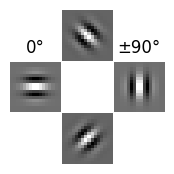
\includegraphics[scale=0.8, max width=\linewidth]{./fig/bayesian-brain/neural-sampling/cell007.png}
	\caption{cell007.png}
	\label{cell007.png}
\end{figure}
とする.元論文では$F, \bar{F}$が定義されていたが,$F=0$とするため,以後の式から削除した.

$$
\begin{array}{l}
\mathbf{P} :=\left[\begin{array}{cc}
\mathbf{P}_{11} & \mathbf{P}_{12} \\
\mathbf{P}_{12} & \mathbf{P}_{22}
\end{array}\right] := E\left[\mathbf{X} \mathbf{X}^\top\right] \\
\mathbf{V} :=\left[\begin{array}{cc}
\mathbf{Q}+\mathbf{L}^\top R \mathbf{L} & -\mathbf{L}^\top R \mathbf{L} \\
\begin{itemize}
\item\mathbf{L}^\top R \mathbf{L} & \mathbf{L}^\top R \mathbf{L}+\mathbf{U}
\end{itemize}
\end{array}\right]
\end{array}
$$

$$
\begin{aligned}
&K=\mathbf{P}_{22} \mathbf{C}^\top\left(\mathbf{D} \mathbf{D}^\top\right)^{-1} \\
&\mathbf{L}=\left(R+\mathbf{Y}^\top\left(\mathbf{S}_{11}+\mathbf{S}_{22}\right) \mathbf{Y}\right)^{-1} \mathbf{B}^\top \mathbf{S}_{11} \\
&\bar{\mathbf{A}}^\top \mathbf{S}+\mathbf{S} \bar{\mathbf{A}}+\bar{\mathbf{Y}}^\top \mathbf{S} \bar{\mathbf{Y}}+\mathbf{V}=0 \\
&\bar{\mathbf{A}} \mathbf{P}+\mathbf{P} \bar{\mathbf{A}}^\top+\bar{\mathbf{Y}} \mathbf{P} \bar{\mathbf{Y}}^\top+\bar{\mathbf{G}} \bar{\mathbf{G}}^\top=0
\end{aligned}
$$


$\mathbf{A} = (a_{ij})$ を $m \times n$ 行列,$\mathbf{B} = (b_{kl})$ を $p \times q$ 行列とすると、それらのクロネッカー積 $\mathbf{A} \otimes \mathbf{B}$ は

$$
\mathbf{A}\otimes \mathbf{B}={\begin{bmatrix}a_{11}\mathbf{B}&\cdots &a_{1n}\mathbf{B}\\\vdots &\ddots &\vdots \\a_{m1}\mathbf{B}&\cdots &a_{mn}\mathbf{B}\end{bmatrix}}
$$

で与えられる $mp \times nq$ 区分行列である.

Roth's column lemma (vec-trick) 

$$
(\mathbf{B}^\top \otimes \mathbf{A})\text{vec}(\mathbf{X}) = \text{vec}(\mathbf{A}\mathbf{X}\mathbf{B})=\text{vec}(\mathbf{C})
$$

によりこれを解くと,

$$
\begin{aligned}
\mathbf{S} &= -\text{vec}^{-1}\left(\left(\mathbf{I} \otimes \bar{\mathbf{A}}^\top + \bar{\mathbf{A}}^\top \otimes \mathbf{I} + \bar{\mathbf{Y}}^\top \otimes \bar{\mathbf{Y}}^\top\right)^{-1}\text{vec}(\mathbf{V})\right)\\
\mathbf{P} &= -\text{vec}^{-1}\left(\left(\mathbf{I} \otimes \bar{\mathbf{A}} + \bar{\mathbf{A}} \otimes \mathbf{I} + \bar{\mathbf{Y}} \otimes \bar{\mathbf{Y}}\right)^{-1}\text{vec}(\bar{\mathbf{G}}\bar{\mathbf{G}}^\top)\right)
\end{aligned}
$$

となる.ここで$\mathbf{I}=\mathbf{I}^\top$を用いた.

\lstinputlisting[language=julia]{./text/introduction/linear-regression/009.jl}
\lstinputlisting[language=julia]{./text/introduction/linear-regression/010.jl}
\begin{figure}[ht]
	\centering
	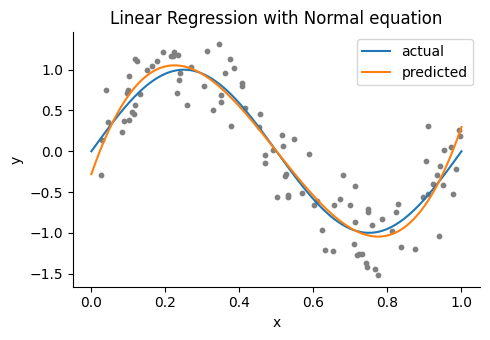
\includegraphics[scale=0.8, max width=\linewidth]{./fig/introduction/linear-regression/cell010.png}
	\caption{cell010.png}
	\label{cell010.png}
\end{figure}
 % ok
% \section{確率論}
\subsection{期待値 (Expectation)}
\begin{equation}
\mathbb{E}_{x\sim p(x)}\left[f(x)\right]\coloneqq \int f(x)p(x)dx
\end{equation}
$x\sim p(x)$ が明示的な場合は $\mathbb{E}_{p(x)}\left[f(x)\right]$ や $\mathbb{E}\left[f(x)\right]$ と表す.
\subsection{情報量 (Information)}
出現頻度が低い事象は多くの情報量を持つ (Shannon, 1948).
\begin{equation}
\mathbb{I}(x)\coloneqq \ln\left(\frac{1}{p(x)}\right)=-\ln p(x)
\end{equation}
$\mathbf{I}$は単位行列なので注意.
\subsection{平均情報量 (エントロピー, entropy)}
\begin{align}
\mathbb{H}(x)&\coloneqq \mathbb{E}[-\ln p(x)]\\
\mathbb{H}(x\vert y)&\coloneqq \mathbb{E}[-\ln p(x\vert y)]
\end{align}
\subsection{Kullback-Leibler 情報量}
Kullback-Leibler (KL) divergence (Kullback and Leibler, 1951)
\begin{align}
D_{\text{KL}}\left(p(x) \Vert\ q(x)\right)&\coloneqq \int p(x) \ln \frac{p(x)}{q(x)} dx\\
&=\int p(x) \ln p(x) dx-\int p(x) \ln q(x) dx\\
&=\mathbb{E}_{x\sim p(x)}[\ln p(x)]-\mathbb{E}_{x\sim p(x)}[\ln q(x)]\\
&=-\mathbb{H}(x)-\mathbb{E}_{x\sim p(x)}[\ln q(x)]
\end{align}
\subsection{相互情報量 (Mutual information)}
aaa
 % ok
% \section{確率過程と確率微分方程式}
aaa
 % ok

\chapter{神経細胞のモデル}
% \section{神経細胞の形態と生理}
 % ok
\section{Hodgkin-Huxleyモデル}
\subsection{Hodgkin-Huxleyモデル}
\textbf{Hodgkin-Huxleyモデル}\index{Hodgkin-Huxleyもでる@Hodgkin-Huxleyモデル} (HH モデル)は, ニューロンの膜興奮を表現する,初めに導出された数理モデルである \citep{Hodgkin1952-gy}\footnote{\citep{Hopper2022-xj}はHodgkinおよびHuxleyの論文の図をカラー化して分かりやすくしたものである.}.HodgkinおよびHuxleyはヤリイカの巨大神経軸索に対して\textbf{電位固定法}\index{でんいこていほう@電位固定法}(voltage-clamp)を用いた実験を行い, 実験から得られた観測結果を元にモデルを構築した \citep{Schwiening2012-pi}.HHモデルには等価な電気回路モデルがあり, \textbf{膜の並列等価回路モデル}\index{まくのへいれつとうかかいろもでる@膜の並列等価回路モデル} (parallel conductance model)と呼ばれている.膜の並列等価回路モデルでは, ニューロンの細胞膜をコンデンサ, 細胞膜に埋まっているイオンチャネルを可変抵抗 (動的に変化する抵抗) として置き換える.

\textbf{イオンチャネル}\index{いおんちゃねる@イオンチャネル} (ion channel)は特定のイオン(例えばナトリウムイオンやカリウムイオンなど)を選択的に通す膜輸送体の一種である.それぞれのイオンの種類において, 異なるイオンチャネルがある (同じイオンでも複数の種類のイオンチャネルがある).また, イオンチャネルにはイオンの種類に応じて異なる\textbf{コンダクタンス}\index{こんだくたんす@コンダクタンス}(抵抗の逆数で電流の「流れやすさ」を意味する)と\textbf{平衡電位}\index{へいこうでんい@平衡電位}(equilibrium potential)がある.HHモデルでは, ナトリウム(Na$^{+}$)チャネル, カリウム(K$^{+}$)チャネル, 漏れ電流(leak current)のイオンチャネルを仮定する.漏れ電流のイオンチャネルは当時特定できなかったチャネルで, 膜から電流が漏れ出すチャネルを意味する.なお, 現在では漏れ電流の多くはCl$^{-}$イオン(chloride ion)によることが分かっている.
それでは, 等価回路モデルを用いて電位変化の式を立ててみよう.上図において, $C_m$は細胞膜のキャパシタンス(膜容量), $I_{m}(t)$は細胞膜を流れる電流(外部からの入力電流), $I_\text{Cap}(t)$は膜のコンデンサを流れる電流, $I_\text{Na}(t)$及び $I_K(t)$はそれぞれナトリウムチャネルとカリウムチャネルを通って膜から流出する電流, $I_\text{L}(t)$は漏れ電流である.このとき, 


\begin{equation}
I_{m}(t)=I_\text{Cap}(t)+I_\text{Na}(t)+I_\text{K}(t)+I_\text{L}(t)    
\end{equation}


という仮定をしている.膜電位を$V(t)$とすると, Kirchhoffの第二法則 (Kirchhoff's Voltage Law)より, 


\begin{equation}
\underbrace{C_m\frac {dV(t)}{dt}}_{I_\text{Cap} (t)}=I_{m}(t)-I_\text{Na}(t)-I_\text{K}(t)-I_\text{L}(t)
\end{equation}


となる.Hodgkinらはチャネル電流$I_\text{Na}, I_K, I_\text{L}$が従う式を実験的に求めた.


\begin{align}
I_\text{Na}(t) &= \bar{g}_{\text{Na}}\cdot m^{3}h(V-E_{\text{Na}})\\
I_\text{K}(t) &= \bar{g}_{\text{K}}\cdot n^{4}(V-E_{\text{K}})\\
I_\text{L}(t) &= \bar{g}_{\text{L}}(V-E_{\text{L}})
\end{align}


ただし, $\bar{g}_{\text{Na}}, \bar{g}_{\text{K}}$はそれぞれNa$^+$, K$^+$の最大コンダクタンスである (ここで上付き棒は上限値であることを示す).$\bar{g}_{\text{L}}$はオームの法則に従うコンダクタンスで, Lコンダクタンスは時間的に変化はしないと仮定する.また, $m$はNa$^+$コンダクタンスの活性化パラメータ, $h$はNa$^+$コンダクタンスの不活性化パラメータ, $n$はK$^+$コンダクタンスの活性化パラメータであり, ゲートの開閉確率を表している.よって, HHモデルの状態は$V, m, h, n$の4変数で表される.これらの変数は以下の$x$を$m, n, h$に置き換えた3つの微分方程式に従う. 


\begin{equation}
\frac{dx}{dt}=\alpha_{x}(V)(1-x)-\beta_{x}(V)x
\end{equation}


ただし, $V$の関数である$\alpha_{x}(V),\ \beta_{x}(V)$は$m, h, n$によって異なり, 次の6つの式に従う.


\begin{equation}
\begin{array}{ll}
\alpha_{m}(V)=\dfrac {0.1(V+40)}{1-\exp (-0.1(V+40))}, &\beta_{m}(V)=4\exp {(-(V+65)/18)}\\
\alpha_{h}(V)=0.07\exp {(-0.05(V+65))}, & \beta_{h}(V)=1/(1+{\exp {\left(-0.1(V+35)\right)}})\\
\alpha_{n}(V)={\dfrac {0.01(V+55)}{1-\exp {\left(-0.1(V+55)\right)}}},& \beta_{n}(V)=0.125\exp {(-0.0125(V+65))} 
\end{array}
\end{equation}


これまでに説明した式を用いてHHモデルを実装する.まず必要なパッケージを読み込む.
\lstinputlisting[language=julia]{./text/neuron-model/hodgkin-huxley/002.jl}
\lstinputlisting[language=julia]{./text/neuron-model/hodgkin-huxley/003.jl}
変更しない定数を保持する \jl{struct} の \jl{HHParameter} と, 変数を保持する \jl{mutable struct} の \jl{HH} を作成する.定数は次のように設定する. 


\begin{equation}
\begin{array}{l}
C_m=1.0\ \mu\textrm{F/cm}^2, \bar{g}_{\text{Na}}=120\ \textrm{mS/cm}^2, \bar{g}_{\text{K}}=36\ \textrm{mS/cm}^2, \bar{g}_{\text{L}}=0.3\ \textrm{mS/cm}^2\\
E_{\text{Na}}=50.0\ \textrm{mV}, E_{\text{K}}=-77\ \textrm{mV}, E_{\text{L}}=-54.387\ \textrm{mV} 
\end{array}
\end{equation}

\lstinputlisting[language=julia]{./text/neuron-model/hodgkin-huxley/005.jl}
\lstinputlisting[language=julia]{./text/neuron-model/hodgkin-huxley/006.jl}
次に変数を更新する関数\jl{update!}を書く.ソルバーとしては陽的Euler法または4次のRunge-Kutta法を用いる.以下ではEuler法を用いている.Juliaではforループを用いて1つのニューロンごとにパラメータを更新する方がベクトルを用いるよりも高速である.
\subsubsection{Hodgkin-Huxleyモデルのシミュレーションの実行}
いくつかの定数を設定してシミュレーションを実行する.
\lstinputlisting[language=julia]{./text/neuron-model/hodgkin-huxley/009.jl}
ニューロンの膜電位 \jl{v}, ゲート変数 \jl{m, h, n}, 刺激電流 \jl{Ie}の描画をする.
\lstinputlisting[language=julia]{./text/neuron-model/hodgkin-huxley/011.jl}
\begin{figure}[ht]
	\centering
	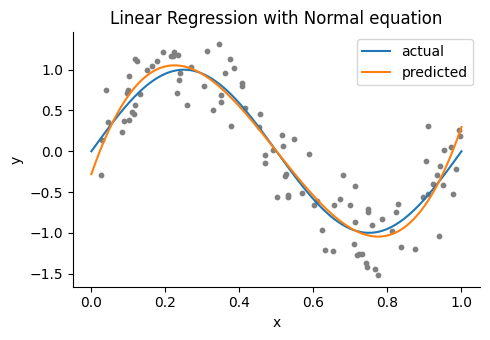
\includegraphics[scale=0.8, max width=\linewidth]{./fig/introduction/linear-regression/cell011.png}
	\caption{cell011.png}
	\label{cell011.png}
\end{figure}
次項で用いるために発火回数を求める.ここでは膜電位が0を超えた点を数えることで,簡易的に求める.
\lstinputlisting[language=julia]{./text/neuron-model/hodgkin-huxley/013.jl}
50msから200msまでで11回, 250msから400msまでで16回発火しているので発火回数は計27回であり,この結果は正しい.
\subsection{Connor-Stevensモデル}
HHモデルはイカの巨大軸索の活動を再現したものであるが,脊椎動物のニューロンの神経活動を再現するためにHHモデルを修正したモデル (modified Hodgkin-Huxley model) が提案されてきた.その一種である,\textbf{Connor-Stevensモデル}\index{Connor-Stevensもでる@Connor-Stevensモデル} はHHモデルに2つ目のカリウム電流 (A型カリウム電流) を追加し,低い発火率でも活動を維持できる (振動を維持できる) ようにしたものである \citep{Connor1971-rs,Connor1977-qo}.ここでパラメータは\citep{Dayan2005-ib}に記載のものを使用する.


\begin{equation}
\begin{array}{l}
C_m=1.0\ \mu\textrm{F/cm}^2,\\ 
\bar{g}_{\text{Na}}=120\ \textrm{mS/cm}^2, \bar{g}_{\text{K}}=20\ \textrm{mS/cm}^2, \bar{g}_{\text{A}}=47.7\ \textrm{mS/cm}^2, \bar{g}_{\text{L}}=0.3\ \textrm{mS/cm}^2\\
E_{\text{Na}}=55.0\ \textrm{mV}, E_{\text{K}}=-72\ \textrm{mV}, E_{\text{A}}=-75\ \textrm{mV},E_{\text{L}}=-17\ \textrm{mV} 
\end{array}
\end{equation}



\begin{equation}
\begin{array}{ll}
\alpha_m=\dfrac{0.38(V+29.7)}{1-\exp (-0.1(V+29.7))} & \beta_m=15.2 \exp (-(V+54.7)/18) \\
\alpha_h=0.266 \exp (-0.05(V+48)) & \beta_h=3.8 /(1+\exp (-0.1(V+18))) \\ 
\alpha_n=\dfrac{0.02(V+45.7)}{1-\exp (-0.1(V+45.7))} & \beta_n=0.25 \exp (-0.0125(V+55.7))
\end{array}
\end{equation}



\begin{equation}
\frac{dx}{dt}=\frac{x_\infty-x}{\tau_x}\ (x=a, b)
\end{equation}



\begin{equation}
\begin{array}{l}
a_{\infty}=\left(\dfrac{0.0761 \exp [(V+94.22)/31.84]}{1+\exp ((V+1.17)/28.93)}\right)^{\frac{1}{3}}\\
\tau_a=0.3632+1.158 /(1+\exp ((V+55.96)/20.12)) \\
b_{\infty}=\left[1+\exp ((V+53.3)/14.54)\right]^{-4}\\
\tau_b=1.24+2.678 /(1+\exp [(V+50)/16.027])
\end{array}
\end{equation}
\lstinputlisting[language=julia]{./text/neuron-model/hodgkin-huxley/016.jl}
\lstinputlisting[language=julia]{./text/neuron-model/hodgkin-huxley/017.jl}
\lstinputlisting[language=julia]{./text/neuron-model/hodgkin-huxley/018.jl}
\lstinputlisting[language=julia]{./text/neuron-model/hodgkin-huxley/019.jl}
\begin{figure}[ht]
	\centering
	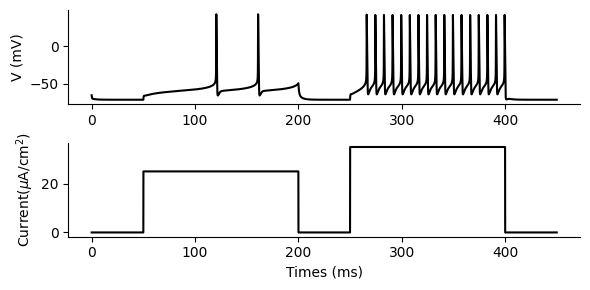
\includegraphics[scale=0.8, max width=\linewidth]{./fig/neuron-model/hodgkin-huxley/cell019.png}
	\caption{cell019.png}
	\label{cell019.png}
\end{figure}
\subsection{F-I曲線}
HHモデルにおいて,入力電流に対する発火率がどのように変化するかを調べる.次のコードのように入力電流を徐々に増加させたときの発火率を見てみよう.
\lstinputlisting[language=julia]{./text/neuron-model/hodgkin-huxley/021.jl}
\lstinputlisting[language=julia]{./text/neuron-model/hodgkin-huxley/022.jl}
発火率を計算して結果を描画する.
\lstinputlisting[language=julia]{./text/neuron-model/hodgkin-huxley/024.jl}
\begin{figure}[ht]
	\centering
	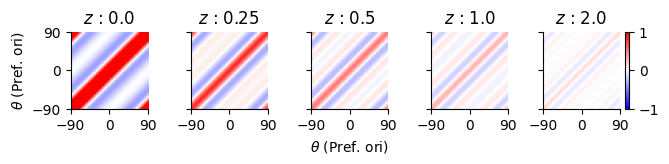
\includegraphics[scale=0.8, max width=\linewidth]{./fig/bayesian-brain/neural-sampling/cell024.png}
	\caption{cell024.png}
	\label{cell024.png}
\end{figure}
このような曲線を\textbf{frequency-current (F-I) 曲線}\index{frequency-current (F-I) きょくせん@frequency-current (F-I) 曲線} (または neuronal input/output (I/O) 曲線)と呼ぶ.$I_\theta$は閾値電流を意味する (ここでは発火率が1Hz以上になる点を閾値と設定している) .F-I曲線の種類に応じてType IおよびIIに分けられる\footnote{Type IIIニューロンも存在する}.
\subsection{全か無かの法則の反例}
ニューロンは電流が流入することで膜電位が変化し, 膜電位がある一定の閾値を超えると活動電位が発生する, というのはニューロンの活動電位発生についての典型的な説明である.膜電位が閾値を超えるか超えないかで活動電位の発生が決まるという法則を, \textbf{全か無かの法則}\index{まったかなかのほうそく@全か無かの法則} (all-or-none principle) と呼ぶ.後に説明するLIFモデルなどは,全か無かの法則に従って神経活動のモデル化を行っている.しかし,この全か無かの法則の法則は必ずしも成立するわけではない.反例として \textbf{抑制後リバウンド}\index{よくせいのちりばうんど@抑制後リバウンド} (Postinhibitory rebound; PIR)という現象がある.抑制後リバウンドは過分極性の電流の印加を止めた際に膜電位が静止膜電位に回復するのみならず, さらに脱分極をして発火をするという現象である.この時生じる発火を\textbf{リバウンド発火}\index{りばうんどはっか@リバウンド発火} (rebound spikes)と呼ぶ.この現象が生じる要因として\textbf{アノーダルブレイク}\index{あのーだるぶれいく@アノーダルブレイク} (anodal break, またはanode break excitation; ABE)や,遅いT型カルシウム電流 (slow T-type calcium current) が考えられている \citep{Chik2004-ka}.HH モデルはこのうちアノーダルブレイクを再現できるため, シミュレーションによりどのような現象か確認してみよう.これは入力電流を変更するだけで行える.
\lstinputlisting[language=julia]{./text/neuron-model/hodgkin-huxley/027.jl}
結果は次のようになる.
\lstinputlisting[language=julia]{./text/neuron-model/hodgkin-huxley/029.jl}
\begin{figure}[ht]
	\centering
	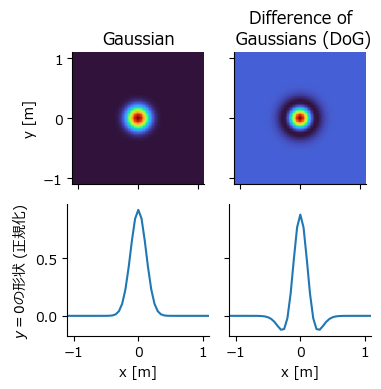
\includegraphics[scale=0.8, max width=\linewidth]{./fig/local-learning-rule/pca-hebbian-learning/cell029.png}
	\caption{cell029.png}
	\label{cell029.png}
\end{figure}
なぜこのようなことが起こるか, というと過分極の状態から静止膜電位へと戻る際にNa$^+$チャネルが活性化 (Na$^+$チャネルの活性化パラメータ$m$が増加し, 不活性化パラメータ$h$が減少)し, 膜電位が脱分極することで再度Na$^+$チャネルが活性化する, というポジティブフィードバック過程(\textbf{自己再生的過程}\index{じこさいせいてきかてい@自己再生的過程})に突入するためである (もちろん, この過程は通常の活動電位発生のメカニズムである). この際, 発火に必要な閾値が膜電位の低下に応じて下がった, ということもできる.

なお,PIRに関連する現象として抑制後促通 (Postinhibitory facilitation; PIF)がある.これは抑制入力の後に興奮入力がある一定の時間内で入ると発火が起こるという現象である \citep{Dodla2006-fj}.

% \section{FitzHugh-Nagumoモデル}
\subsection{FitzHugh-Nagumoモデルの定義}

前節では神経活動のダイナミクスを微分方程式で表したHodgkin-Huxley(HH)モデルを扱った.HHモデルの特徴は,4変数で構成され,各変数が膜電位およびNaチャネルやKチャネルなどの活性/不活性状態を意味することである.このHHモデルをより簡易化し,2変数で神経活動の興奮とその伝播を表そうと提案されたのが\textbf{FitzHugh-Nagumo (FHN)モデル}\index{FitzHugh-Nagumo (FHN)もでる@FitzHugh-Nagumo (FHN)モデル} である.FHNモデルはvan der Pol振動子をFitzHughが修正し\cite{FitzHugh1955-bx} \cite{Fitzhugh1961-fp},南雲らによりトンネル (江崎) ダイオードを用いて電子回路上に実装\footnote{神経活動を再現する電子回路を\textbf{ニューリスタ}\index{にゅーりすた@ニューリスタ}  (neuristor) という.}された \cite{Nagumo1962-ob}という経緯がある.FHNモデルは以下で表される.


\begin{align} 
\frac{dv}{dt} &= c\left(v-\frac{v^3}{3}-u+I_e\right)\\ 
\frac{du}{dt} &= v-bu+a 
\end{align}


$v$は膜電位で,$u$は回復変数(recovery variable)と呼ばれる. FitzHughにより,HHモデルにおける$(V, m)$および$(n, h)$がそれぞれFHNモデルの$v$および$u$に対応すると説明されている \cite{Fitzhugh1961-fp} \footnote{HHモデルにおける$V$と$m$は強い正の相関があり,$n$と$h$は強い負の相関があるため,それぞれの変数の組は1つの変数に縮約されうる.}.$a,b,c$は定数であり,$a=0.7, b=0.8, c=10$がよく使われる.$I_e$は外部刺激電流に対応する.
\lstinputlisting[language=julia]{./text/neuron-model/fhn/001.jl}
変更しない定数を保持する \jl{struct} の \jl{FHNParameter} と, 変数を保持する \jl{mutable struct} の \jl{FHN} を作成する.
\lstinputlisting[language=julia]{./text/neuron-model/fhn/003.jl}
次に変数を更新する関数\jl{update!}を書く.ソルバーとしては陽的Euler法または4次のRunge-Kutta法を用いる.以下ではEuler法を用いている.Juliaではforループを用いて1つのニューロンごとにパラメータを更新する方がベクトルを用いるよりも高速である.
\lstinputlisting[language=julia]{./text/neuron-model/fhn/005.jl}
\subsection{FitzHugh-Nagumoモデルのシミュレーションの実行}
いくつかの定数を設定してシミュレーションを実行する.
\lstinputlisting[language=julia]{./text/neuron-model/fhn/007.jl}
結果を描画する.
\lstinputlisting[language=julia]{./text/neuron-model/fhn/009.jl}
\begin{figure}[ht]
	\centering
	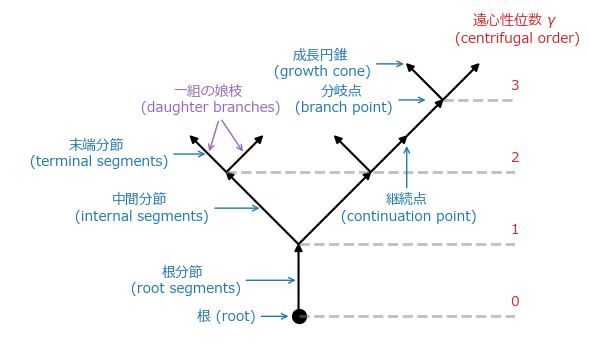
\includegraphics[scale=0.8, max width=\linewidth]{./fig/neuron-model/neurite-growth-model/cell009.png}
	\caption{cell009.png}
	\label{cell009.png}
\end{figure}
\subsection{相図の描画}
phase plot
\lstinputlisting[language=julia]{./text/neuron-model/fhn/011.jl}
\lstinputlisting[language=julia]{./text/neuron-model/fhn/012.jl}
\begin{figure}[ht]
	\centering
	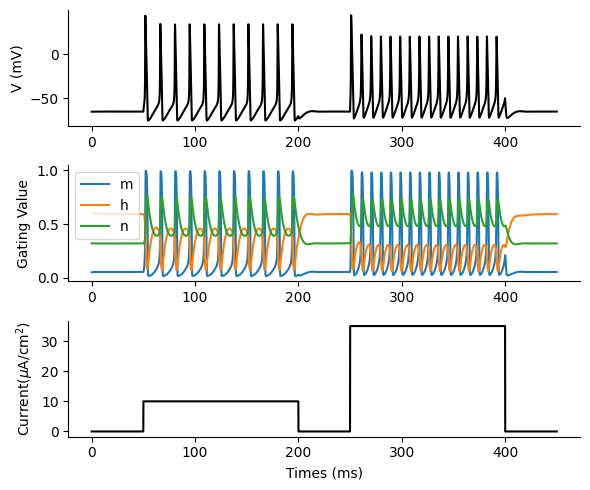
\includegraphics[scale=0.8, max width=\linewidth]{./fig/neuron-model/hodgkin-huxley/cell012.png}
	\caption{cell012.png}
	\label{cell012.png}
\end{figure}

% \section{Leaky integrate-and-fire モデル}
\subsection{LIFモデルの定義}
生理学的なイオンチャネルの挙動は考慮せず, 入力電流を膜電位が閾値に達するまで時間的に積分するというモデルを\textbf{\index{Integrate-and-fire (IF, せきぶんはっか)もでる@Integrate-and-fire (IF, 積分発火)モデル}} という.さらに, IFモデルにおいて膜電位の漏れ(leak)\footnote{この漏れはイオンの拡散などによるもの. }も考慮したモデルを \textbf{\index{Leaky integrate-and-fire (LIF, もれせきぶんはっか) もでる@Leaky integrate-and-fire (LIF, 漏れ積分発火) モデル}} と呼ぶ.ここではLIFモデルのみを取り扱う.

ニューロンの膜電位を$V_m(t)$, 静止膜電位を$V_\text{rest}$, 入力電流\footnote{シナプス入力による電流がどうなるかは,第三章「シナプス伝達のモデル」で扱う.}を$I(t)$, 膜抵抗を$R_m$, 膜電位の時定数を$\tau_m\ (=R_m \cdot C_m)$とすると, 式は次のようになる\footnote{$(V_{m}(t)-V_\text{rest})$の部分は膜電位の基準を静止膜電位としたことにして, 単に$V_m(t)$だけの場合もある. また, 右辺の$RI(t)$の部分は単に$I(t)$とされることもある. 同じ表記だが, この場合の$I(t)$はシナプス電流に比例する量, となっている(単位はmV). }.


\begin{equation}
\tau_m \frac{dV_{m}(t)}{dt}=-(V_{m}(t)-V_\text{rest})+R_mI(t)
\end{equation}


ここで, $V_m$が閾値(threshold)\footnote{thから始まるので文字$\theta$が使われることもある.}$V_{\text{th}}$を超えると, 脱分極が起こり, 膜電位はピーク電位 $V_{\text{peak}}$まで上昇する.発火後は再分極が起こり, 膜電位はリセット電位 $V_{\text{reset}}$まで低下すると仮定する\footnote{リセット電位は静止膜電位と同じ場合もあれば, 過分極を考慮して静止膜電位より低めに設定することもある.}.発火後, 一定の期間$\tau_{\text{ref}}$ の間は膜電位が変化しない\footnote{実装によっては不応期の間は膜電位の変化は許容するが発火は生じないようにすることもある.} とする.これを \textbf{\index{ふおうき(refractory time period)@不応期(refractory time period)}} と呼ぶ.

以上を踏まえてLIFモデルを実装してみよう.まず必要なパッケージを読み込む.
\lstinputlisting[language=julia]{./text/neuron-model/lif/001.jl}
HHモデルと同様に変更しない定数を保持する \jl{struct} の \jl{LIFParameter} と, 変数を保持する \jl{mutable struct} の \jl{LIF} を作成する.
\lstinputlisting[language=julia]{./text/neuron-model/lif/003.jl}
次に変数を更新する関数\jl{update!}を書く.
\lstinputlisting[language=julia]{./text/neuron-model/lif/005.jl}
いくつかの処理について解説しておく.まず,一番目のforループ内の\jl{v[i]}の\jl{((dt*tcount) > (tlast[i] + tref))}は最後にニューロンが発火した時刻\jl{tlast[i]}に不応期\jl{tref}を足した時刻よりも現在の時刻\jl{dt*tcount[1]}が大きければ膜電位の更新を許可し,小さければ更新しない.二番目のforループにおける\jl{fire[i]}はニューロンの膜電位が閾値電位\jl{vthr}を超えたら\jl{True}となる.\jl{v[i]}などの更新式にある\jl{ifelse(a, b, c)}はaが\jl{True}の時はbを返し,\jl{False}の時はcを返す関数であり,\jl{v[i] = ifelse(fire[i], vreset, v[i])}は\jl{fire[i]}が\jl{True}なら\jl{v[i]}をリセット電位\jl{vreset}とし,そうでなければそのままの値を返すという処理である.同様にして\jl{tlast[i]}は発火したときにその時刻を記録する変数となっている.なお,\jl{v_[i] = ifelse(fire[i], vpeak, v[i])}は実際のシミュレーションにおいて意味をなさない.単に発火時の電位\jl{vpeak}を含めて記録すると描画時の見栄えが良いというだけである.

これらの\jl{struct}と関数を用いてシミュレーションを実行する.\jl{I} はHHモデルのときと同じように矩形波を入力する.実は\jl{I}は入力電流ではなく入力電流に比例する量となっているが,これは膜抵抗を乗じた後の値であると考えるとよい.
\subsection{LIFモデルのシミュレーションの実行}
いくつかの定数を設定してシミュレーションを実行する.
\lstinputlisting[language=julia]{./text/neuron-model/lif/008.jl}
発火時電位を含む膜電位\jl{v_}と入力電流\jl{I}を描画する.
\lstinputlisting[language=julia]{./text/neuron-model/lif/010.jl}
\begin{figure}[ht]
	\centering
	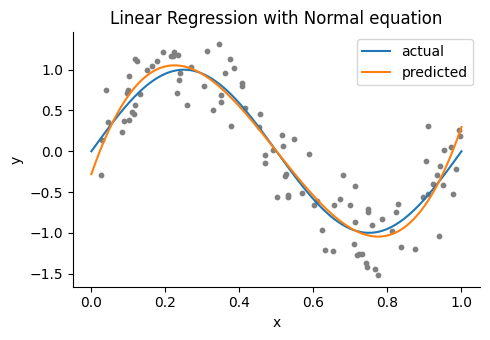
\includegraphics[scale=0.8, max width=\linewidth]{./fig/introduction/linear-regression/cell010.png}
	\caption{cell010.png}
	\label{cell010.png}
\end{figure}
\subsection{LIFモデルのF-I curve}
\subsubsection{数値的計算によるF-I curveの描画}
この項目ではLIFモデルにおける入力電流に対する発火率の変化 (F-I curve)を描画する.方法はHHモデルの場合と同様だが,今回は発火したかどうかがモデル内の変数として明示的に記録されているので処理が少ない.
\lstinputlisting[language=julia]{./text/neuron-model/lif/012.jl}
発火率を計算し,描画する.
\lstinputlisting[language=julia]{./text/neuron-model/lif/014.jl}
\lstinputlisting[language=julia]{./text/neuron-model/lif/015.jl}
\begin{figure}[ht]
	\centering
	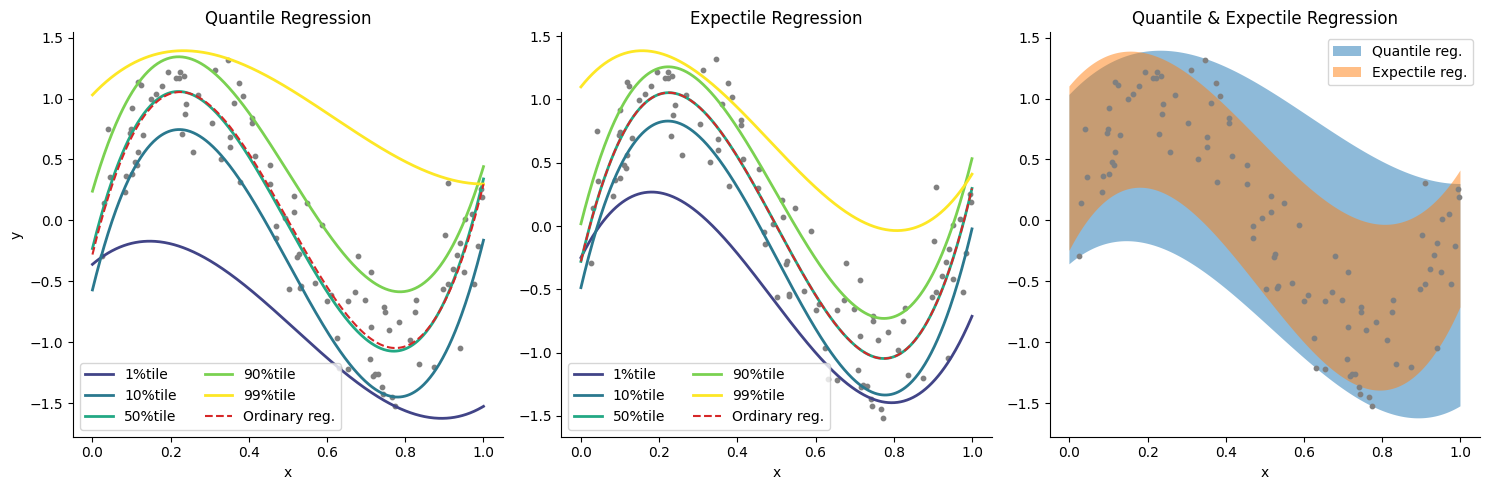
\includegraphics[scale=0.8, max width=\linewidth]{./fig/bayesian-brain/quantile-expectile-regression/cell015.png}
	\caption{cell015.png}
	\label{cell015.png}
\end{figure}
さらに電流を強めると発火率は飽和(saturation)する.なお,不応期がない,すなわち0の場合は閾値付近以外はReLU関数のような挙動をする.
\subsubsection{解析的計算によるF-I curveの描画}
ここまでは数値的なシミュレーションによりF-I curveを求めた.以下では解析的にF-I curveの式を求めよう.具体的には,一定かつ持続的な入力電流を$I$としたときのLIFニューロンの発火率(firing rate)が


\begin{equation}
\text{rate}\approx \left(\tau_m \ln \frac{R_mI}{R_mI+V_\text{rest}-V_{\text{th}}}\right)^{-1}
\end{equation}


と近似できることを示す.まず,$t=t_1$にスパイクが生じたとする.このとき, 膜電位はリセットされるので$V_m(t_1)=V_\text{rest}$である(リセット電位と静止膜電位が同じと仮定する).$[t_1, t]$における膜電位はLIFの式を積分することで得られる.


\begin{equation}
\tau_m \frac{dV_{m}(t)}{dt}=-(V_{m}(t)-V_\text{rest})+R_m I
\end{equation}


の式を積分すると, 


\begin{align}
\int_{t_1}^{t} \frac{\tau_m dV_m}{R_mI+V_\text{rest}-V_m}&=\int_{t_1}^{t} dt\\
\ln \left(1-\frac{V_m(t)-V_\text{rest}}{R_mI}\right)&=-\frac{t-t_1}{\tau_m} \quad (\because V_m(t_1)=V_\text{rest})\\
V_m(t) &=V_\text{rest} + R_mI\left[1-\exp\left(-\frac{t-t_1}{\tau_m}\right)\right] 
\end{align}


となる.$t>t_1$における初めのスパイクが$t=t_2$に生じたとすると, そのときの膜電位は$V_m(t_2)=V_{\text{th}}$である (実際には閾値以上となっている場合もあるますが近似する).$t=t_2$を上の式に代入して


\begin{align}
V_{\text{th}}&=V_\text{rest} + R_mI\left[1-\exp\left(-\frac{t_2-t_1}{\tau}\right)\right] \\
T&= t_2-t_1 = \tau_m \ln \frac{R_mI}{R_mI+V_\text{rest}-V_{\text{th}}}
\end{align}


となる.ここで$T$は2つのスパイクの時間間隔 (spike interval)である.$t_1\leq t<t_2$におけるスパイクは$t=t_1$時の1つなので, 発火率は$1/T$となる.よって


\begin{equation}
\text{rate}\approx \frac{1}{T}=\left(\tau_m \ln \frac{R_mI}{R_mI+V_\text{rest}-V_{\text{th}}}\right)^{-1}
\end{equation}


となる.不応期$\tau_{\text{ref}}$を考慮すると, 持続的に入力がある場合は単純に$\tau_{\text{ref}}$だけ発火が遅れるので発火率は$1/(\tau_{\text{ref}}+T)$となる.

それではこの式に基づいてF-I curveを描画してみよう.
\lstinputlisting[language=julia]{./text/neuron-model/lif/018.jl}
\jl{log}の中身が0になるとErrorが生じるので3項演算子で場合分けをしている.なお,\jl{1e3}を乗じているのは1/msからHzに変換するためである.結果は次のようになる.数値的な計算結果とほぼ一致していることがわかる.
\lstinputlisting[language=julia]{./text/neuron-model/lif/020.jl}
\begin{figure}[ht]
	\centering
	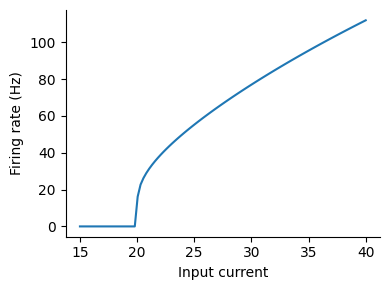
\includegraphics[scale=0.8, max width=\linewidth]{./fig/neuron-model/lif/cell020.png}
	\caption{cell020.png}
	\label{cell020.png}
\end{figure}
 % ok
% \section{Izhikevich モデル}
\subsection{Izhikevich モデルの定義}
\textbf{\index{Izhikevich もでる@Izhikevich モデル}} (または\textbf{\index{Simple model}})は([Izhikevich, 2003](https://www.izhikevich.org/publications/spikes.htm))で考案されたモデルである.HHモデルのような生理学的な知見に基づいたモデルは実際のニューロンの発火特性をよく再現できるが,式が複雑化するため,数学的な解析が難しく,計算量が増えるために大規模なシミュレーションも困難となる\footnote{これに関しては必ずしも正しくない.計算機の発達によりHHモデルで大きなモデルをシミュレーションすることも可能である.}.そこで,生理学的な正しさには目をつぶり,生体内でのニューロンの発火特性を再現するモデルが求められた.その特徴を持つのがIzhikevich モデルである (以下ではIzモデルと表記する).Izモデルは 2変数しかない\footnote{数値計算をする上では簡易的だが,if文が入るために解析をするのは難しくなる.([Bernardo, et al., 2008](https://www.springer.com/gp/book/9781846280399))を読むといいらしい.}
簡素な微分方程式だが, 様々なニューロンの活動を模倣することができる.定式化には主に2種類ある.まず,([Izhikevich, 2003](https://www.izhikevich.org/publications/spikes.htm))で提案されたのが次式である.


\begin{align}
\frac{dv(t)}{dt}&=0.04v(t)^2 + 5v(t)+140-u(t)+I(t) \\
\frac{du(t)}{dt}&=a(bv(t)-u(t))
\end{align} 


ここで,$v$と$u$が変数であり, $v$は膜電位(membrane potential;単位はmV), $u$は回復電流(recovery current; 単位はpA)\footnote{ここでの「回復」というのは脱分極した後の膜電位が静止膜電位へと戻る,という意味である (対義語はactivationで膜電位の上昇を意味する).$u$は$v$の導関数において$v$の上昇を抑制するように$-u$で入っているため,$u$としてはK$^+$チャネル電流やNa$^+$チャネルの不活性化動態などが考えられる.}
である.また,$a$は回復時定数(recovery time constant; 単位はms$^{-1}$)の逆数 (これが大きいと$u$が元に戻る時間が短くなる), $b$は$u$の$v$に対する感受性(共鳴度合い,  resonance; 単位はpA/mV)である.

この式は簡便だが,生理学的な意味づけが分かりにくい.改善された式として["Dynamical Systems in Neuroscience" (Izhikevich, 2007)](https://mitpress.mit.edu/books/dynamical-systems-neuroscience)のChapter 8で紹介されているのが次式である.


\begin{align}
C\frac{dv(t)}{dt}&=k\left(v(t)-v_r\right)\left(v(t)-v_t\right)-u(t)+I(t) \\
\frac{du(t)}{dt}&=a\left\{b\left(v(t)-v_{r}\right)-u(t)\right\}
\end{align} 


ここで,$C$は膜容量(membrane capacitance; 単位はpF), $v_r$は静止膜電位(resting membrane potential; 単位はmV), $v_t$は閾値電位(instantaneous threshold potential; 単位はmV), $k$はニューロンのゲインに関わる定数で,小さいと発火しやすくなる (単位はpA/mV).以後はこちらの式を用いる.

Izモデルの\textbf{\index{いきちのとりあつかい@閾値の取り扱い}}はLIFモデルと異なり,HHモデルに近い.LIFモデルでは閾値を超えた時に膜電位をピーク電位まで上昇させ (この過程は無くてもよい),続いて膜電位をリセットする.Izモデルの閾値は$v_t$だが, 膜電位のリセットは閾値を超えたかで判断せず,膜電位$v$がピーク電位$v_{\text{peak}}$になったとき (または超えた時) に行う.そのためIzモデルの実際の閾値は膜電位の挙動が変化する(発火状態に移行する),つまり分岐(bifurcation) が生じる点であり,パラメータの閾値$v_t$との間には差異がある.

さて,膜電位がピーク電位$v_{\text{peak}}$に達したとき (すなわち \jl{if} $v \geq v_{\text{peak}}$),$u, v$を次のようにリセットする\footnote{バースト発火(bursting)の挙動を表現するためには,速い回復変数(fast recovery variable)と遅い回復変数(slow recovery variable)の2つが必要となる(従って膜電位も合わせて全部で3変数必要).一方で,IzモデルではLIFモデルのようなif文によるリセットを用いているため,速い回復変数が必要なく,遅い回復変数$u$のみでバースト発火を表現できる.}.


\begin{align} 
u&\leftarrow u+d\\
v&\leftarrow v_{\text{reset}}
\end{align}


とする.ただし, $v_{\text{reset}}$は過分極を考慮して静止膜電位$v_r$よりも小さい値とする.また,$d$はスパイク発火中に活性化される正味の外向き電流の合計を表し,発火後の膜電位の挙動に影響する (単位はpA).

以上を踏まえて, シミュレーションを行う.まず,必要なパッケージを読み込む.
\lstinputlisting[language=julia]{./text/neuron-model/izhikevich/001.jl}
変更しない定数を保持する\jl{struct}の\jl{IZParameter}と,変数を保持する\jl{mutable struct}の\jl{IZ}を作成する.2つの定式化でパラメータの値が異なるので注意すること.
\lstinputlisting[language=julia]{./text/neuron-model/izhikevich/003.jl}
次に変数を更新する関数\jl{update!}を書く.LIFの場合と異なり,\jl{v[i] >= vpeak}であることに注意する (\jl{v[i] >= vthr}ではない).
\lstinputlisting[language=julia]{./text/neuron-model/izhikevich/005.jl}
\subsection{Izhikevich モデルのシミュレーションの実行}
いくつかの定数を設定してシミュレーションを実行する.
\lstinputlisting[language=julia]{./text/neuron-model/izhikevich/007.jl}
\jl{Plots}を読み込み,膜電位\jl{v}, 回復変数\jl{u}, 入力電流\jl{I}を描画する.
\lstinputlisting[language=julia]{./text/neuron-model/izhikevich/009.jl}
\begin{figure}[ht]
	\centering
	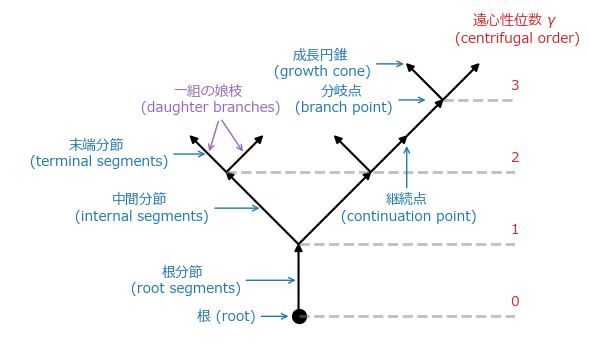
\includegraphics[scale=0.8, max width=\linewidth]{./fig/neuron-model/neurite-growth-model/cell009.png}
	\caption{cell009.png}
	\label{cell009.png}
\end{figure}
\subsection{様々な発火パターンのシミュレーション}
次に様々な発火パターンを模倣するようにIzモデルの定数を変化させてみよう.Intrinsically Bursting (IB)ニューロンとChattering (CH) ニューロン(または fast rhythmic bursting (FRB) ニューロン)のシミュレーションを行う.基本的には定数を変えるだけである.

本書で用いている式における発火パターンに対するパラメータは([Izhikevich, 2003](https://www.izhikevich.org/publications/spikes.htm))では得られないが,["Dynamical Systems in Neuroscience" (Izhikevich, 2007)](https://mitpress.mit.edu/books/dynamical-systems-neuroscience)には記載がある.他の発火パターンに関してはこの本を参照のこと.
\lstinputlisting[language=julia]{./text/neuron-model/izhikevich/011.jl}
これまでと異なり,モデルの定義時に\jl{param}を設定していることに注意しよう.最後に膜電位変化を描画する.
\lstinputlisting[language=julia]{./text/neuron-model/izhikevich/013.jl}
\begin{figure}[ht]
	\centering
	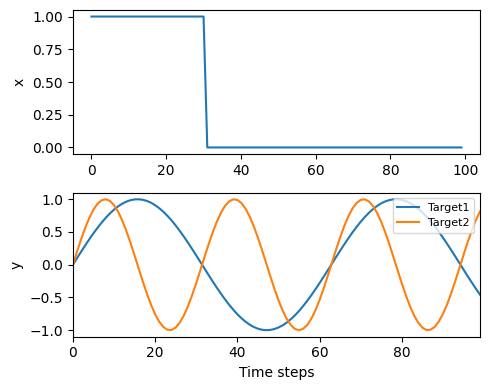
\includegraphics[scale=0.8, max width=\linewidth]{./fig/solve-credit-assignment-problem/bptt/cell013.png}
	\caption{cell013.png}
	\label{cell013.png}
\end{figure}
\subsection{ランダムネットワークのシミュレーション}
1000個のIzニューロン(興奮性800個, 抑制性200個)によるランダムネットワークのシミュレーションを行う.これは([Izhikevich, 2003](https://www.izhikevich.org/publications/spikes.htm))においてMATLABコードが示されており,それをJuliaに移植したものである.このシミュレーションではRS(regular spiking)ニューロンを興奮性細胞,FS(fast spiking)ニューロンを抑制性細胞のモデルとして用いている.
\lstinputlisting[language=julia]{./text/neuron-model/izhikevich/015.jl}
膜電位の更新の際,\jl{v}を2回に分けて更新しているが,これは数値的な安定性を高めるためである.計算量は上がるが,前述したモデルにおいても同様の処理を行う実装もある.

シミュレーションの実行後,ネットワークを構成するニューロンの発火を描画する.これを\textbf{\index{らすたーぷろっと@ラスタープロット}} (raster plot)という.この図は横軸が時間,縦軸がニューロンの番号となっており,各ニューロンが発火したことを点で表している.
\lstinputlisting[language=julia]{./text/neuron-model/izhikevich/017.jl}
\begin{figure}[ht]
	\centering
	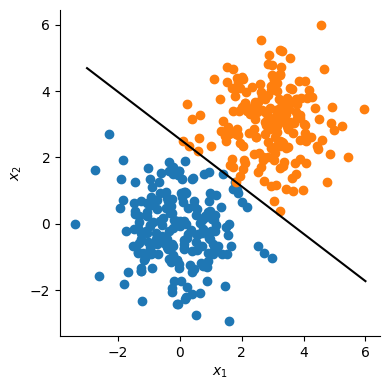
\includegraphics[scale=0.8, max width=\linewidth]{./fig/local-learning-rule/logistic-regression-perceptron/cell017.png}
	\caption{cell017.png}
	\label{cell017.png}
\end{figure}
初めの400msぐらいまでは100msごとに約10Hzの$\alpha$波が見られ,800ms付近には約40Hzの$\gamma$波が見られる.
 
% \section{Inter-spike interval モデル}
これまで紹介したモデルでは,入力に対する膜電位などの時間変化に基づき発火が起こるかどうか,ということを考えてきた.この節では,発火が生じるまでの過程を考慮せず,発火の時間間隔(\textbf{\index{inter-spike interval, ISI}})の統計による現象論的モデルを考える.これを\textbf{\index{Inter-spike interval (ISI)}} モデルと呼ぶ.ISIモデルは\textbf{\index{てんかてい(point process)@点過程(point process)}} という統計的モデルに基づいており,各モデルにはISIが従う分布の名称がついている.

この節では,使用頻度の高い \textbf{\index{ぽあそんかてい (Poisson process) もでる@ポアソン過程 (Poisson process) モデル}},ポアソン過程モデルにおいて不応期を考慮した \textbf{\index{しにどきかんつきぽあそんかてい (Poisson process with dead time, PPD) もでる@死時間付きポアソン過程 (Poisson process with dead time, PPD) モデル}},皮質の定常発火においてポアソン過程モデルよりも当てはまりがよいとされる \textbf{\index{がんまかてい (Gamma process) もでる@ガンマ過程 (Gamma process) モデル}}について説明する.

なお,SNNにおいて,ISIモデルは主に画像入力の際に\textbf{\index{れんぞくちからすぱいくれつへのえんこーど@連続値からスパイク列へのエンコード}}に用いられる.これに限らず入力として用いられることが多い.


この節は 島崎, "スパイク統計モデル入門"\url{https://www.neuralengine.org/res/book/index.html}; Pachitariu, Probabilistic models for spike trains of single neurons \url{http://www.gatsby.ucl.ac.uk/~marius/papers/SpikTrainStats.pdf} を特に参考にした.
\subsection{ポアソン過程モデル}
\subsubsection{点過程とポアソン過程}
時間に応じて変化する確率変数のことを\textbf{\index{かくりつかてい(stochastic process)@確率過程(stochastic process)}} という.さらに確率過程の中で,連続時間軸上において離散的に生起する点事象の系列を\textbf{\index{てんかてい(point process)@点過程(point process)}} という.スパイクは離散的に起こるので,点過程を用いてモデル化ができるという話である.

ポアソン過程 (Poisson process)は点過程の1つである.ポアソン過程モデルはスパイクの発生をポアソン過程でモデル化したもので,このモデルによって生じるスパイクをポアソンスパイク(Poisson spike)と呼ぶ.ポアソン過程では,時刻$t$までに起こった点の数$N(t)$はポアソン分布に従う.すなわち,点が起こる確率が強度$\lambda$のポアソン分布に従う場合, 時刻$t$までに事象が$n$回起こる確率は$P[N(t)=n]=\dfrac{(\lambda t)^{n}}{n !} e^{-\lambda t}$となる. 

ポアソン過程において点が起こる回数がポアソン分布に従うことは,ポアソン過程という名称の由来となっている.これを定義とする場合もあれば,次の4条件を満たす点過程をポアソン過程とするという定義もある.

\begin{itemize}
\item 時刻0における初期の点の数は0 : $P[N(0)=0]=1$ 
\item $[t, t+\Delta t)$に点が1つ生じる確率 : $P[N(t+\Delta t)-N(t)=1]=\lambda(t)\Delta t+o(\Delta t)$
\item 微小時間$\Delta t$の間に点は2つ以上生じない : $P[N(t+\Delta t)-N(t)=2]=o(\Delta t)$
\item 任意の時点$t_1 < t_2 < \cdots< t_n$に対して,増分 $N(t_2)-N(t_1), N(t_3)-N(t_2), \cdots, N(t_n)-N(t_{n−1})$は互いに独立である.
\end{itemize}

ただし, $o(\cdot)$はLandauの記号(Landauのsmall o)であり, $o(x)$は$x\to 0$のとき,$o(x)/x\to 0$となる微小な量を表す.ポアソン過程に従ってスパイクが生じるとする場合,条件2の強度関数$\lambda(t)$は\textbf{\index{はっかりつ@発火率}}を意味する (また実装において有用).条件3は不応期より小さいタイムステップにおいては,1つのタイムステップにおいて1つしかスパイクは生じないということを表す.条件4はスパイクは独立に発生する,ということを意味する.また,これらの条件から$N(t)$の分布は強度母数$\lambda(t)$のポアソン分布に従うことが示せる.

強度関数(点がスパイクの場合,発火率)が$\lambda(t)=\lambda$ (定数)となる場合は点の時間間隔(点がスパイクの場合,ISI)の確率変数$T$が強度母数$\lambda$の \textbf{\index{しすうぶんぷ@指数分布}}に従う.なお,指数分布の確率密度関数は確率変数を$T$とするとき,


\begin{equation}
f(t;\lambda )=\left\{{\begin{array}{ll}\lambda e^{-\lambda t}&(t\geq 0)\\0&(t<0)\end{array}}\right.
\end{equation}


となる.このことは4条件とChapman-Kolmogorovの式により求められるが,ややこしいので, $P[N(t)=n]=\dfrac{(\lambda t)^{n}}{n !} e^{-\lambda t}$から導出できることを簡単に示す.指数分布の累積分布関数を$F(t; \lambda)$とすると,


\begin{equation}
F(t; \lambda) = P(T< t)=1-P(T\geq t)=1-P(N(t)=0)=1-e^{-\lambda t}
\end{equation}


となる.よって


\begin{equation}
f(t; \lambda)=\frac{dF(t; \lambda)}{dt}=\lambda e^{-\lambda t}
\end{equation}


が成り立つ.
\subsubsection{定常ポアソン過程}
ここからポアソン過程によるスパイクのシミュレーションを実装する.実装方法にはISIが指数分布に従うことを利用したものと,ポアソン過程の条件2を利用したものの2通りがある.実装は後者が楽で計算量も少ないが,後のガンマ過程のために前者の実装を先に行う.

\paragraph{ISIの累積により発火時刻を求める手法}
ISIが指数分布に従うことを利用してポアソン過程モデルの実装を行う.まずISIを指数分布に従う乱数とする.次にISIを累積することで発火時刻を得る.最後に発火時間を整数値に丸めてindexとすることで$\{0, 1\}$のスパイク列が得られる.ISIの取得には\jl{Random.randexp()}を用いる.この関数は scale 1の指数分布に従う乱数を返す.このscaleは指数分布の確率密度関数を$f(t; \frac{1}{\beta}) = \frac{1}{\beta} e^{-t/\beta}$とした際の$\beta = 1/\lambda$である(この時,平均は$\beta$となる).よって発火率を\jl{fr}(1/s), 単位時間を\jl{dt}(s)としたときのISIは \jl{isi = 1/(fr*dt) * randexp()}として得ることができる.

まず必要なパッケージを読み込む.
\lstinputlisting[language=julia]{./text/neuron-model/isi/003.jl}
乱数のseed値を設定し,必要な定数を定義した後に\jl{isi}を計算する.\jl{isi}を累積することでスパイクの生じた時刻を記録する配列\jl{spike_time}を作成する.作成後,\jl{spike_time}を用いてラスタープロットを描画する.
\lstinputlisting[language=julia]{./text/neuron-model/isi/005.jl}
\lstinputlisting[language=julia]{./text/neuron-model/isi/006.jl}
\begin{figure}[ht]
	\centering
	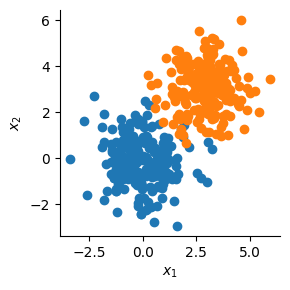
\includegraphics[scale=0.8, max width=\linewidth]{./fig/local-learning-rule/logistic-regression-perceptron/cell006.png}
	\caption{cell006.png}
	\label{cell006.png}
\end{figure}
\jl{spike_time}のように発火時刻で記録しておく方がメモリを節約できるが,シミュレーションにおいてはスパイク列$S$はタイムステップごとに発火しているかを表す$\{0,1\}$配列で保持しておくと楽に扱うことができる.そのため冗長ではあるが,発火時刻の配列を$\{0,1\}$配列\jl{spikes}に変換しスパイクの数と発火率を計算する.
\lstinputlisting[language=julia]{./text/neuron-model/isi/008.jl}
\paragraph{$\Delta t$ 間の発火確率が $\lambda\Delta t$ であることを利用する方法}
次に2番目のポアソン過程モデルの実装を行う.こちらは$\lambda$を発火率とした場合, 区間$[t, t+\Delta t)$の間にポアソンスパイクが発生する確率は$\lambda \Delta t$となることを利用する.これはポアソン過程の条件だが,ポアソン分布から導けることを簡単に示しておく.事象が起こる確率が強度$\lambda$のポアソン分布に従う場合, 時刻$t$までに事象が$n$回起こる確率は$P[N(t)=n]=\dfrac{(\lambda t)^{n}}{n !} e^{-\lambda t}$となる.よって, 微小時間$\Delta t$において事象が$1$回起こる確率は


\begin{equation}
P[N(\Delta t)=1]=\dfrac{\lambda \Delta t}{1 !} e^{-\lambda \Delta t}\simeq \lambda \Delta t+o(\Delta t)
\end{equation}


となる.ただし, $e^{-\lambda \Delta t}$についてはマクローリン展開による近似を行っている.このことから, 一様分布$U(0,1)$に従う乱数$\xi$を取得し, $\xi<\lambda dt$なら発火$(y=1)$, それ以外では$(y=0)$となるようにすればポアソンスパイクを実装できる.
\lstinputlisting[language=julia]{./text/neuron-model/isi/010.jl}
\lstinputlisting[language=julia]{./text/neuron-model/isi/011.jl}
\lstinputlisting[language=julia]{./text/neuron-model/isi/012.jl}
\begin{figure}[ht]
	\centering
	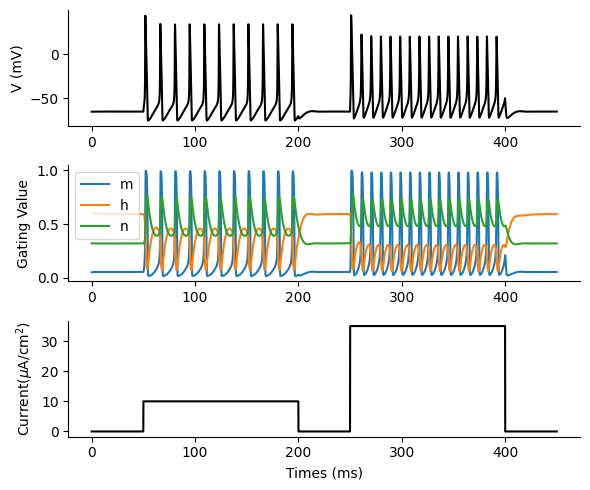
\includegraphics[scale=0.8, max width=\linewidth]{./fig/neuron-model/hodgkin-huxley/cell012.png}
	\caption{cell012.png}
	\label{cell012.png}
\end{figure}
なお,ここでは全時間における発火をまとめて計算しているが,タイムステップごとに発火の有無を計算することもできる.前者は発火情報を保持するためのメモリが必要だが,計算時間は短くなる.後者はメモリの節約になるが,計算時間は長くなる.そのため,これら2つの方法はメモリと計算時間のトレードオフとなる.また,他には発火情報を疎行列(sparse matrix)の形式で保持しておくとメモリの節約になると思われる.
\subsubsection{非定常ポアソン過程}
これまでの実装は発火率$\lambda$が一定であるとする,定常ポアソン過程 (homogeneous poisson process)であったが,ここからは発火率$\lambda(t)$が時間変化するとする\textbf{\index{ひていじょうぽあそんかてい@非定常ポアソン過程}} (inhomogeneous poisson process)について考える.とはいえ,定常ポアソン過程における発火率を,時間についての関数で置き換えるだけで実装できる.以下は$\lambda(t)=\sin^2(\alpha t)$(ただし$\alpha$は定数)とした場合の実装である.
\lstinputlisting[language=julia]{./text/neuron-model/isi/015.jl}
\begin{figure}[ht]
	\centering
	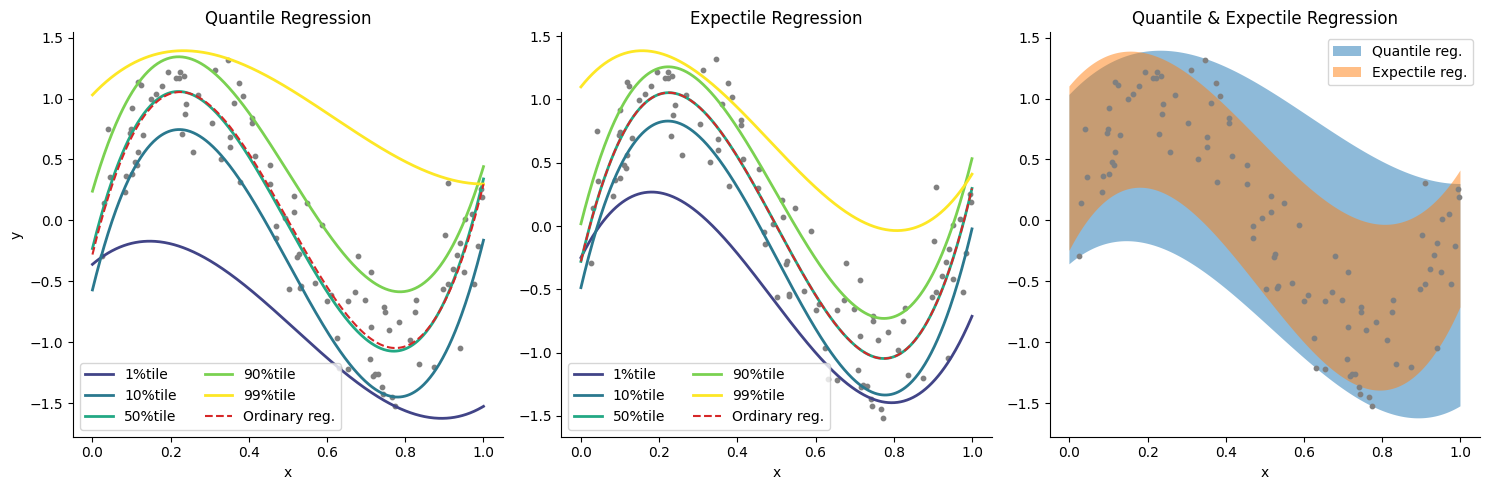
\includegraphics[scale=0.8, max width=\linewidth]{./fig/bayesian-brain/quantile-expectile-regression/cell015.png}
	\caption{cell015.png}
	\label{cell015.png}
\end{figure}
上が発火率$\lambda(t)$の時間変化, 下がラスタープロットである.
\subsection{死時間付きポアソン過程モデル (Poisson process with dead time, PPD)}
ポアソン過程は簡易的で有用だが,不応期を考慮していない.そのため,時には生理的範疇を超えたバースト発火が起こる場合もある (複数のニューロンからの発火の重ね合わせ(superposition)であると考えることもできる.) .そこで,ポアソン過程において不応期のようなイベントの生起が起こらない \textbf{\index{しにどきかん(dead time)@死時間(dead time)}} \footnote{例えば,ガイガー・カウンター(Geiger counter)などの放射線の検出器には放射線の到達を機器の物理的特性として検出できない時間(つまり死時間)がある.そのため放射線の到達数がポアソン分布に従うとした場合,放射線測定装置のモデルとしてPPDが用いられる.}を考慮した\textbf{\index{しにどきかんつきぽあそんかてい (Poisson process with dead time, PPD)@死時間付きポアソン過程 (Poisson process with dead time, PPD)}} (またはdead time modified Poisson process)というモデルを導入する.

実装においてはLIFニューロンの時と同じような不応期の処理をする.つまり,現在が不応期かどうかを判断し,不応期なら発火を許可しないようにする.
\lstinputlisting[language=julia]{./text/neuron-model/isi/018.jl}
不応期があるために発火率は設定値の30Hzよりも低くなっていることが分かる.次にラスタープロットを描画する.
\lstinputlisting[language=julia]{./text/neuron-model/isi/020.jl}
\begin{figure}[ht]
	\centering
	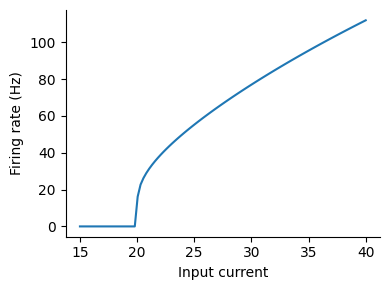
\includegraphics[scale=0.8, max width=\linewidth]{./fig/neuron-model/lif/cell020.png}
	\caption{cell020.png}
	\label{cell020.png}
\end{figure}
通常のPoisson spikeと差はあまり感じられないが,高頻度発火の場合に通常のモデルとの違いが明瞭となる.
\subsection{ガンマ過程モデル}
ガンマ過程(gamma process)は点の時間間隔がガンマ分布に従うとするモデルである.ガンマ過程はポアソン過程よりも皮質における定常発火への当てはまりが良いとされている
\begin{itemize}
\item Shinomoto, et al., 2003 \url{https://pubmed.ncbi.nlm.nih.gov/14629869/}
\item Maimon and Assad,2009 \url{https://pubmed.ncbi.nlm.nih.gov/19447097/}
\end{itemize}

時間間隔の確率変数を$T$とした場合,ガンマ分布の確率密度関数は


\begin{equation}
f(t;k,\theta) =  t^{k-1}\frac{e^{-t/\theta}}{\theta^k\Gamma(k)}
\end{equation}


と表される.ただし,$t > 0$であり, 2つの母数は$k, \theta > 0$である.また,$\Gamma (\cdot)$はガンマ関数であり,


\begin{equation}
\Gamma (k)=\int _{0}^{\infty }x^{k-1}e^{-x}\,dx
\end{equation}


と定義される.ガンマ分布の平均は$k\theta$だが,発火率はISIの平均の逆数なので,$\lambda=1/k\theta$となる.また,$k=1$のとき,ガンマ分布は指数分布となる.さらに$k$が正整数のとき,ガンマ分布はアーラン分布となる.

ガンマ過程モデルの実装はポアソン過程モデルのISIを累積する手法と同様に書くことができる.ただしこの時,Distributions.jl \url{https://github.com/JuliaStats/Distributions.jl} を用いる.基本的には\jl{randexp(shape)}を\jl{rand(Gamma(a,b), shape)}に置き換えればよい (もちろん多少の修正は必要とする).
スパイク列を生成する関数を書く.
\lstinputlisting[language=julia]{./text/neuron-model/isi/024.jl}
\jl{gamma_spike} 関数を用いて $k=1, 12$ の場合のシミュレーションを実行する.なお,$k=1$のときはポアソン過程に一致することに注意しよう.
\lstinputlisting[language=julia]{./text/neuron-model/isi/026.jl}
ISIの分布を描画するための関数を定義する.
\lstinputlisting[language=julia]{./text/neuron-model/isi/028.jl}
結果を描画する.上段はISIの分布,下段はラスタープロットである.左の$k=1$の場合をポアソン過程モデルのスパイク列と比較しよう (同じ外観になっていることが分かる).右は$k=12$とした場合である.
\lstinputlisting[language=julia]{./text/neuron-model/isi/030.jl}
\begin{figure}[ht]
	\centering
	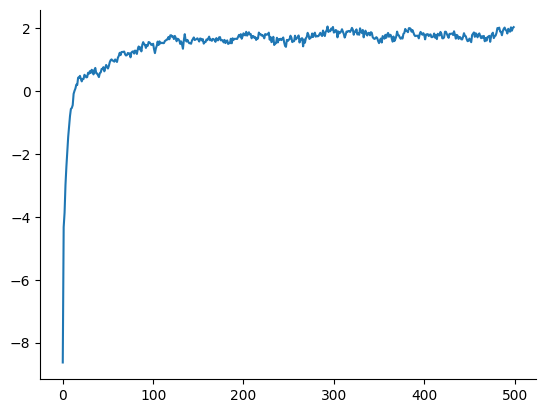
\includegraphics[scale=0.8, max width=\linewidth]{./fig/bayesian-brain/mcmc/cell030.png}
	\caption{cell030.png}
	\label{cell030.png}
\end{figure}
なお,前述したようにガンマ過程モデルの方がポアソン過程モデルよりも皮質ニューロンのモデルとしては優れているが,入力画像のエンコーディングをガンマ過程モデルにすることでSNNの認識精度が向上するかどうかはまだ十分に研究されていない.また,(Deger, et al., 2012\url{https://pubmed.ncbi.nlm.nih.gov/21964584/})ではPPDやガンマ過程の重ね合わせによるスパイク列を生成するアルゴリズムを考案している.
 % ok
% \section{神経突起の成長モデル}
神経細胞は他の細胞に比して特異な形態を持つ.またニューロンの種類およびその役割により基本的な細胞体,樹状突起,軸索等の構造は共通するものの,各部分の形態は異なる.このような形態はどのようにして発達するのだろうか.本節では\textbf{神経突起(neurite)}\index{しんけいとっき(neurite)@神経突起(neurite)} の\textbf{成長モデル(growth model)}\index{せいちょうもでる(growth model)@成長モデル(growth model)} を取り扱う.神経突起とは神経細胞において細胞体から伸びる突起の総称である.
\subsection{神経突起の木構造}
神経突起の形態は\textbf{樹状}\index{じゅじょう@樹状}突起 (dendrites; ギリシャ語で木を意味する*déndron*に由来) に代表されるように (生物としての) 木に類似している.さらに分節(segment)に離散化することでグラフ理論における\textbf{木}\index{き@木}(tree; 連結で閉路を持たないグラフ)として捉えることができる.

シミュレーション用にデータ構造を作成しよう.なお,Juliaで木構造を扱うためのライブラリ\jl{AbstractTrees.jl}は使用しない.\jl{tree_info}はInt型vector (要素数3) のlistであり,接続している分節の番号,遠心性位数,分節の種類(1: 末端, 0:中間)を表す.\jl{seg_vec}は Float型vector (要素数2) のlistであり,分節の2次元極座標ベクトル(半径,角度)を表す.3次元に拡張することも可能であるが,本書では簡単のために2次元とする.多次元配列ではなくvectorのlistにしているのは,成長に伴って要素を追加していく際に配列に結合\jl{cat}するよりlist化して追加\jl{push!}する方が高速なためである.
\lstinputlisting[language=julia]{./text/neuron-model/neurite-growth-model/002.jl}
\lstinputlisting[language=julia]{./text/neuron-model/neurite-growth-model/003.jl}
木構造を描画するための関数を作成する.以下の\jl{segments_lines}は\jl{tree_info}と\jl{seg_vec}から節点位置\jl{pos}と各分節の両端点\jl{lines}を返す関数である.\jl{lines}は主に\jl{matplotlib.collections.LineCollection}で用いる (\jl{plot}を用いるより高速である).
\lstinputlisting[language=julia]{./text/neuron-model/neurite-growth-model/005.jl}
\lstinputlisting[language=julia]{./text/neuron-model/neurite-growth-model/006.jl}
木構造を描画してみよう.以下では各部位の説明を加えており,\cite{Koene2009-hv}, \cite{Cuntz2010-in}を参考に作成した.
\lstinputlisting[language=julia]{./text/neuron-model/neurite-growth-model/008.jl}
\lstinputlisting[language=julia]{./text/neuron-model/neurite-growth-model/009.jl}
\begin{figure}[ht]
	\centering
	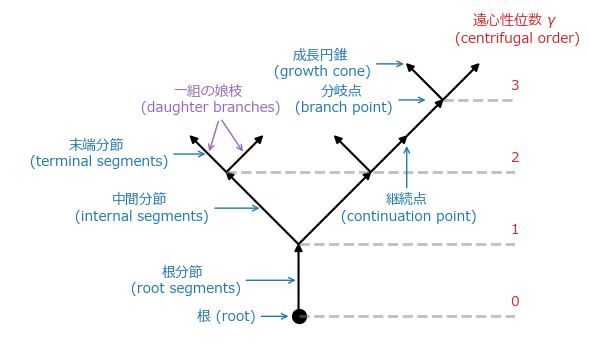
\includegraphics[scale=0.8, max width=\linewidth]{./fig/neuron-model/neurite-growth-model/cell009.png}
	\caption{cell009.png}
	\label{cell009.png}
\end{figure}
\subsection{Van Peltモデル}
Van PeltモデルはVan Peltらによって構築された,神経突起の成長についての現象論的モデルである \cite{Van_Pelt2002-vm}.以下では\cite{Koene2009-hv}に基づいて記述する.なお,このモデルでは軸索誘導分子 (axon guidance molecules) 等の存在は無視している.

神経突起の成長の過程には分岐(branching),伸長(elongation),転向(turn)が含まれる.簡略化のため,空間を2次元にし,分節の太さおよび成長円錐が向きを変える時のsegment history tension model (後述) を省略する.またVan Peltモデルを元にした神経回路構築ソフトウェア\textbf{NETMORPH}\index{NETMORPH} \cite{Koene2009-hv}ではシナプス結合の形成も含めたシミュレーションを行っている.

\subsubsection{分岐 (branching)}
時刻$[t_i, t_i + \Delta t]$において,$j$番目の末端分節(terminal segment)が分岐する確率は


\begin{equation}
p_{i,j} = n_i^{-E}\cdot B_{\infty} e^{\frac{-t_i}{\tau}} \left(e^{\frac{\Delta t}{\tau}} - 1\right)\cdot \frac{2^{-S\gamma_j}}{C_{n_i}}
\end{equation}


で表される.ここで,$B_{\infty}, E, S, \tau$は定数である.$\gamma_j$は$j$番目の末端分節の遠心性位数(centrifugal order)であり,$n_i$は時刻$t_i$における末端分節の総計である.さらに


\begin{equation}
{C_{n_i}} = \frac{1}{n_i}\sum\nolimits_{k = 1}^{n_i} {{2^{ - S{\gamma_k}}}}
\end{equation}


とする.$n_i^{-E}$は末端分節の総計に応じて分岐確率を変化させる項であり,$E$は競合変数(competition parameter)と呼ばれる.
$B_{\infty} e^{\frac{-t_i}{\tau}} \left(e^{\frac{\Delta t}{\tau}} - 1\right)$は経過時間に応じて分岐確率を変化させる項であり,$B_{\infty}$は$E=0$の場合の末端分節での分岐数の漸近的な期待値である.
$\frac{2^{-S\gamma_j}}{C_{n_i}}$の項は末端分節の遠心性位数に応じて分岐確率を変化させる項であり,$C_{n_i}$は正規化定数である.
$S=0$のときは末端分節は全て同じ確率で分岐するが,$S>0$のときは近位の末端分節,$S<0$のときは遠位の末端分節における分岐確率が大きくなる.
\lstinputlisting[language=julia]{./text/neuron-model/neurite-growth-model/011.jl}
\subsubsection{伸長 (elongation) }
末端分節が伸長する速さ$\nu_e(t_i)\ [\mu m/s]$は正規分布 $\mathcal{N}(\mu_e, \sigma_e^2)$に従うとする \cite{Van_Ooyen2014-fb}.伸長する長さは$\Delta L_j(t_i)=\nu_e(t_i) \cdot \Delta t$となる.

\subsubsection{転向 (turn)}
神経突起は真っ直ぐに伸び続けるわけではなく,向きを時折変えながら伸長する.伸長時に転向するかどうかの確率$p_d(t_i)$を次のようにする.


\begin{equation}
p_d(t_i) = r_L\Delta L_j(t_i)
\end{equation}


ただし,$r_L\ [\mu m^{-1}]$は回転率を表す.確率$p_d(t_i)$により転向する部分は新しい分節として定義する.転向する角度は\cite{Koene2009-hv}では転向角度の履歴を考慮したsegment history tension modelが導入されているが,本書では前述のように省略する.代わりに転向角度は一様分布$U(-\alpha, \alpha)\ \left(\alpha\in \left[0, \frac{\pi}{2}\right]\right)$に従うとする.

分岐した際にも娘枝の長さと角度の設定が必要となる.ここでは長さは末端分節の伸長と同じ正規分布に従うとする.また,分岐角度は2つの娘枝について一様分布$U(0, \beta_1),\ U(-\beta_2, 0)\ \left(\beta_1, \beta_2\in \left[0, \frac{\pi}{2}\right]\right)$にそれぞれ従うとする.

以上をまとめてシミュレーションを実装する.
\lstinputlisting[language=julia]{./text/neuron-model/neurite-growth-model/013.jl}
パラメータを設定する.このパラメータは\cite{Koene2009-hv}, \cite{Van_Ooyen2014-fb}に基づいている.Van Peltモデルにおいて錐体細胞のような複雑な形態を作成するには,各部位に分割してシミュレーションし結合することが必要となる.今回は軸索のパラメータを用いる.
\lstinputlisting[language=julia]{./text/neuron-model/neurite-growth-model/015.jl}
シミュレーションを実行する.
\lstinputlisting[language=julia]{./text/neuron-model/neurite-growth-model/017.jl}
結果を表示する.初めの神経突起の数を2にしていてもそれ以上出ているように見えるのは最初期に分岐しているためである (細胞体を描画しなければ確認できる).
\lstinputlisting[language=julia]{./text/neuron-model/neurite-growth-model/019.jl}
\begin{figure}[ht]
	\centering
	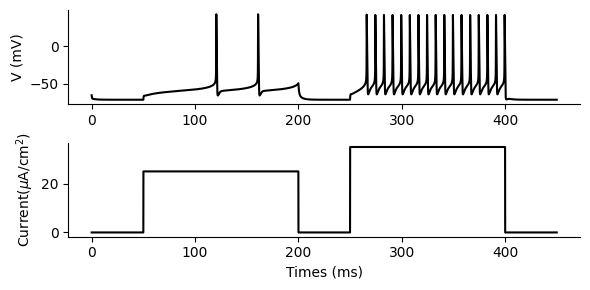
\includegraphics[scale=0.8, max width=\linewidth]{./fig/neuron-model/hodgkin-huxley/cell019.png}
	\caption{cell019.png}
	\label{cell019.png}
\end{figure}
対称性の破れを考慮していないので,円系に成長している.
ToDo: 神経細胞極性についての記述.
 % ok

\printbibliography[segment=\therefsegment,heading=subbibliography,title={参考文献}]
\addcontentsline{toc}{section}{参考文献}
% \printbibliography

\chapter{シナプス伝達のモデル}
% \section{シナプスの形態と生理
}
スパイクが生じたことによる膜電位変化は軸索を伝播し, \textbf{\index{しなぷす@シナプス}}という構造により, 次のニューロンへと興奮が伝わる. このときの伝達の仕組みとして, シナプスには\textbf{\index{かがくしなぷす@化学シナプス}}(chemical synapse)とGap junctionによる\textbf{\index{でんきしなぷす@電気シナプス}}(electrical synapse)がある.  



化学シナプスの場合, シナプス前膜からの\textbf{\index{しんけいでんたつぶっしつ@神経伝達物質}}の放出, シナプス後膜の受容体への神経伝達物質の結合, イオンチャネル開口による\textbf{\index{しなぷすのちでんりゅう@シナプス後電流}}(postsynaptic current; PSC)の発生, という過程が起こる.



しかし, これらの過程を全てモデル化するのは計算量がかなり大きくなるので, 基本的には簡易的な現象論的なモデルを用いる.



このように, シナプス前細胞のスパイク列(spike train)は次のニューロンにそのまま伝わるのではなく, ある種の時間的フィルターをかけられて伝わる.このフィルターを\textbf{\index{しなぷすふぃるたー@シナプスフィルター}}(synaptic filter)と呼ぶ.本章では, このようにシナプス前細胞で生じた発火が, シナプス後細胞の膜電位に与える過程のモデルについて説明する.



 % ok
% \section{Current / Conductance-based シナプス
}
\subsection{化学シナプスの2つの記述形式
}
具体的なシナプスのモデルの前に,この節では化学シナプスにおけるシナプス入力(synaptic drive)の2つの形式,\textbf{Current-based シナプス}\index{Current-based しなぷす@Current-based シナプス}と\textbf{Conductance-based シナプス}\index{Conductance-based しなぷす@Conductance-based シナプス}について説明する.簡単に言うと,Current-based シナプスは入力電流が変化するというモデルで,Conductance-based シナプスはイオンチャネルのコンダクタンス (電気抵抗の逆数,電流の流れやすさ) が変化するというモデルである \citep{Cavallari2014-jx}.以下では例として,次のLIFニューロンの方程式におけるシナプス入力を考える.
\begin{equation}
\tau_m \frac{dV_{m}(t)}{dt}=-(V_{m}(t)-V_\text{rest})+R_m I_{\text{syn}}(t)    
\end{equation}
ただし,$\tau_m$ は膜電位の時定数,$V_m(t)$ は膜電位,$V_\text{rest}$ は静止膜電位,$R_m$ は膜抵抗である.ここで,シナプス入力の電流$I_{\text{syn}}(t)$ \footnote{シナプス(synapse)入力であることを明らかにするためにsynと添え字をつけている.} が2つのモデルにおいて異なる部分となる.
\subsection{Current-based シナプス
}
Current-based シナプスは単純に\textbf{入力電流が変化}\index{にゅうりょくでんりゅうがへんか@入力電流が変化}するというモデルで,モデルを簡素化したい場合によく用いられる.シナプス入力 $I_{\text{syn}}(t)$はシナプス効率(synaptic efficacy)\footnote{シナプス強度(Synaptic strength)とは違い,受容体の種類(GABA受容体やAMPA受容体,およびそのサブタイプなど)によって決まる.} を $J_{\text{syn}}$ (単位はpA) とし,シナプスの動態(synaptic kinetics)を $s_{\text{syn}}(t)$ とすると,次式のようになる.ただし,シナプスの動態とは前細胞に注目すれば神経伝達物質の放出量,後細胞に注目すれば神経伝達物質の結合量やイオンチャネルの開口率を表す.
\begin{equation}
I_{\text{syn}}(t)=\underbrace{J_{\text{syn}}s_{\text{syn}}(t)}_{電流の変化}    
\end{equation}
ただし,$s_{\text{syn}}(t)$ は,例えば次節で紹介する $\alpha$ 関数を用いる場合, 
\begin{equation}
s_{\text{syn}}(t)=\dfrac{t}{\tau_s} \exp \left(1-\dfrac{t}{\tau_s}\right)    
\end{equation}
のようになる.
\subsection{Conductance-based シナプス
}
Conductance-based シナプスはイオンチャネルの\textbf{コンダクタンスが変化}\index{こんだくたんすがへんか@コンダクタンスが変化}するというモデルである.例えば Hodgkin-Huxley モデルはConductance-based モデルの1つである.Current-basedよりもConductance-based の方が生理学的に妥当である.例えば抑制性シナプスは膜電位が平衡電位と比べて脱分極側にあるか,過分極側にあるかで抑制的に働くか興奮的に働くかが逆転するが,これはCurrent-based シナプスでは再現できない.Conductance-based モデルにおけるシナプス入力は$I_{\text{syn}}(t)$は次のようになる. 
\begin{equation}
I_{\text{syn}}(t)=\underbrace{g_{\text{syn}}s_{\text{syn}}(t)}_{コンダクタンスの変化}\cdot\ \left(V_{\text{syn}}-V_{m}(t)\right)    
\end{equation}
ただし,$g_{\text{syn}}$ (単位はnS)はシナプスの最大コンダクタンス\footnote{$g_{\text{syn}}$がシナプスの最大コンダクタンスとなるのは $s_{\text{syn}}$の最大値を1に正規化する場合である.正規化は必須ではないので,単なる係数と思うのがよい.},$V_{\text{syn}}$ (単位はmV) はシナプスの平衡電位を表す.これらも$J_{\text{syn}}$と同じく,シナプスにおける受容体の種類によって決まる定数である.
注意しなければならないことは,$s_{\text{syn}}(t)\leq 0$としたとき Current-based モデルにおける $J_{\text{syn}}$ は正の値(興奮性)と負の値(抑制性)を取るが,$g_{\text{syn}}$は正の値のみである,ということである\footnote{これはコンダクタンスが電気抵抗の逆数であり,基本的に抵抗は正の値しか取らないことからも分かる.なお電子回路においては素子の抵抗値が見かけ上,負の値を取る場合もあり\textbf{負性抵抗}\index{ふせいていこう@負性抵抗} (negative resistance) と呼ばれる}.Conductance-basedモデルで興奮性と抑制性を決定しているのは,平衡電位$V_{\text{syn}}$である.興奮性シナプスの平衡電位は高く,抑制性シナプスの平衡電位は低いため,膜電位を引いた符号はそれぞれ正と負になる.

% \section{記号の表記
}


本書では次のような記号表記を用いる.

\begin{itemize}
\item 実数全体を$\mathbb{R}$, 複素数全体は$\mathbb{C}$と表記する.

\item スカラーは小文字・斜体で $x$ のように表記する.

\item ベクトルは小文字・立体・太字で $\mathbf{x}$ のように表記し,列ベクトル (縦ベクトル) として扱う.

\item 行列は大文字・立体・太字で $\mathbf{X}$ のように表記する.

\item $n\times 1$の実ベクトルの集合を $\mathbb{R}^n$, $n\times m$ の実行列の集合を $\mathbb{R}^{n\times m}$と表記する.

\item 行列 $\mathbf{X}$ の置換は $\mathbf{X}^\top$と表記する.ベクトルの要素を表す場合は $\mathbf{x} = (x_1, x_2,\cdots, x_n)^\top$のように表記する.

\item 単位行列を $\mathbf{I}$ と表記する.

\item ゼロベクトルは $\mathbf{0}$ , 要素が全て1のベクトルは $\mathbf{1}$ と表記する.  

\item $e$を自然対数の底とし,指数関数を $e^x=\exp(x)$と表記する.また,自然対数を $\ln(x)$と表記する.

\item 定義を$:=$を用いて行う.例えば,$f(x):=2x$は$f(x)$という関数を$2x$として定義するという意味である.

\item 平均 $\mu$, 標準偏差 $\sigma$ の正規分布を $\mathcal{N}(\mu, \sigma^2)$ と表記する.

\end{itemize}


\subsection{変数の命名規則
}


\begin{itemize}
\item \jl{tp1, tm1} : time plus one (t+1), time minus one (t-1)
\end{itemize}

\lstinputlisting[language=julia]{./text/synapse-model/expo-synapse/001.jl}
\lstinputlisting[language=julia]{./text/synapse-model/expo-synapse/002.jl}
\lstinputlisting[language=julia]{./text/synapse-model/expo-synapse/003.jl}
\begin{figure}[ht]
	\centering
	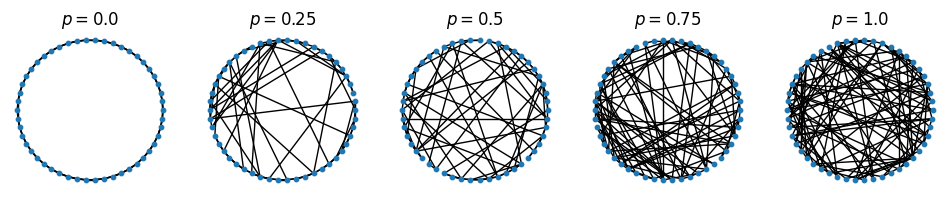
\includegraphics[scale=0.8, max width=\linewidth]{./fig/appendix/graph-theory-network-model/cell003.png}
	\caption{cell003.png}
	\label{cell003.png}
\end{figure}
##  Erdős-Rényi graph
Juliaの余りの関数は \jl{rem(x, y)} と \jl{mod(x, y)}がある.Juliaの\jl{x % y}は\jl{rem}と同じだが,Pythonの場合は\jl{mod}と同じなので注意.

Juliaの余りの関数は \jl{rem(x, y)} と \jl{mod(x, y)}がある.Juliaの\jl{x % y}は\jl{rem}と同じだが,Pythonの場合は\jl{mod}と同じなので注意.

% \section{動力学モデル}
\subsection{チャネル動態の動力学的表現}
指数関数型シナプスとモデルの振る舞いはほぼ同一だが, 式の構成が少し異なるモデルとして\textbf{動力学モデル}\index{どうりきがくもでる@動力学モデル} (Kinetic model, またはMarkov kinetic model)がある \citep{Destexhe1994-ro}.動力学モデルはHHモデルのゲート変数の式と類似した式で表される.このモデルではチャネルが開いた状態(Open)と閉じた状態(Close), および神経伝達物質(neurotransmitter)の放出状態(T)の2つの要素に関する状態がある.また, 閉$\to$開の反応速度を$\alpha$, 開$\to$閉の反応速度を$\beta$とする.このとき,これらを表す状態遷移の式は次のようになる.
\begin{equation}
\text{Close}+\text{T}  \underset{\beta}{\overset{\alpha}{\rightleftharpoons}}\text{Open}    
\end{equation}
ここで, シナプス動態を$r$とすると
\begin{equation}
\frac{dr}{dt}=\alpha T (1-r) - \beta r
\end{equation}
となる.ただし, Tはシナプス前細胞が発火したときにインパルス的に1だけ増加するとする.また, $\alpha, \beta$は速度なので, 時定数の逆数であることに注意しよう. $\alpha=2000 \text{ms}^{-1}$, $\beta=200 \text{ms}^{-1}$とすると, シナプス動態は次のようになる.
\begin{lstlisting}[language=julia]
using PyPlot
rc("axes.spines", top=false, right=false)
\end{lstlisting}
\begin{lstlisting}[language=julia]
dt = 1e-4 # タイムステップ (sec)
α, β = 1/5e-4, 1/5e-3
T = 0.05 # シミュレーション時間 (sec)
nt = Int(T/dt) # シミュレーションの総ステップ

r = zeros(nt)

for t in 1:nt-1
    spike = ifelse(t == 1, 1, 0)
    r[t+1] = r[t] + dt * (α*spike*(1-r[t]) - β*r[t])
end

time = (1:nt)*dt
figure(figsize=(4, 3))
plot(time, r)
xlabel("Time (s)"); ylabel("Post-synaptic current (pA)")
tight_layout()
\end{lstlisting}
\begin{figure}[ht]
	\centering
	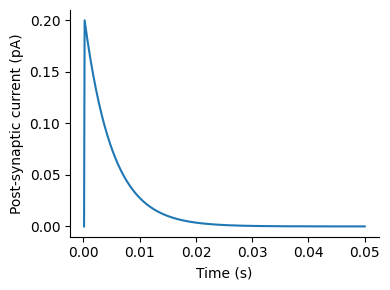
\includegraphics[scale=0.8, max width=\linewidth]{./fig/synapse-model/kinetic-synapse/cell002.png}
	\caption{cell002.png}
	\label{cell002.png}
\end{figure}
\subsection{Hodgkin-Huxleyモデルにおけるシナプスモデル}
これまで明示的にスパイクの発生が表現されたモデルを用いてきたが,HHモデルでは単なる膜電位の変数があるのみである.ここでは前述した動力学的モデルを用いてHHモデルにおけるシナプス動態の記述を行う ([Destexhe et al., 1994](https://www.mitpressjournals.org/doi/10.1162/neco.1994.6.1.14); [Batista et al., 2014](https://www.sciencedirect.com/science/article/pii/S0378437114004592)).
$r_{j}$を$j$番目のニューロンのpre-synaptic dynamicsとすると,$r_{j}$は次式に従う.
\frac{\mathrm{d} r_{j}}{\mathrm{d} t}=\left(\frac{1}{\tau_{r}}-\frac{1}{\tau_{d}}\right) \frac{1-r_{j}}{1+\exp \left(-V_{j}+V_{0}\right)}-\frac{r_{j}}{\tau_{d}}
ただし,時定数 $\tau_r=0.5, \tau_d = 8$ (ms), 反転電位 $V_0 = -20$ (mV)とする.前節で既に$r$の描画は行ったが,パルス波を印加した場合の挙動を確認する.
\begin{lstlisting}[language=julia]
using Parameters: @unpack # or using UnPack

abstract type Layer end
abstract type Neuron <: Layer end
abstract type SpikeNeuron <: Neuron end

abstract type Synapse <: Layer end

@kwdef struct HHParameter{FT}
    Cm::FT = 1 # 膜容量(uF/cm^2)
    gNa::FT = 120; gK::FT = 36; gL::FT = 0.3 # Na+, K+, leakの最大コンダクタンス(mS/cm^2)
    ENa::FT = 50; EK::FT = -77; EL::FT = -54 # Na+, K+, leakの平衡電位(mV)
end

@kwdef mutable struct HH{FT} <: SpikeNeuron
    num_neurons::UInt16
    dt::FT = 1e-3
    param::HHParameter = HHParameter{FT}()
    v::Vector{FT} = fill(-65, num_neurons)
    m::Vector{FT} = fill(0.05, num_neurons) 
    h::Vector{FT} = fill(0.6, num_neurons)
    n::Vector{FT} = fill(0.32, num_neurons)
end

@kwdef struct HHKineticSynapseParameter{FT}
    tr::FT = 0.5; td::FT = 8 # ms
    tr⁻¹::FT = 1/tr; td⁻¹::FT = 1/td
    v₀::FT = -20 # mV
end

@kwdef mutable struct HHKineticSynapse{FT} <: Synapse
    num_neurons::UInt16
    dt::FT = 1e-3
    param::HHKineticSynapseParameter = HHKineticSynapseParameter{FT}()
    r::Vector{FT} = zeros(num_neurons)
end

function update!(neuron::HH, x::Vector)
    @unpack num_neurons, dt, v, m, h, n = neuron
    @unpack Cm, gNa, gK, gL, ENa, EK, EL = neuron.param
    @inbounds for i = 1:num_neurons
        m[i] += dt * ((0.1(v[i]+40)/(1 - exp(-0.1(v[i]+40))))*(1 - m[i]) - 4exp(-(v[i]+65) / 18)*m[i])
        h[i] += dt * ((0.07exp(-0.05(v[i]+65)))*(1 - h[i]) - 1/(1 + exp(-0.1(v[i]+35)))*h[i])
        n[i] += dt * ((0.01(v[i]+55)/(1 - exp(-0.1(v[i]+55))))*(1 - n[i]) - (0.125exp(-0.0125(v[i]+65)))*n[i])
        v[i] += dt / Cm * (x[i] - gNa * m[i]^3 * h[i] * (v[i] - ENa) - gK * n[i]^4 * (v[i] - EK) - gL * (v[i] - EL))
    end
    return v
end

function update!(synapse::HHKineticSynapse, v::Vector)
    @unpack num_neurons, dt, r = synapse
    @unpack tr⁻¹, td⁻¹, v₀ = synapse.param    
    @inbounds for i = 1:num_neurons
        r[i] += dt * ((tr⁻¹ - td⁻¹) * (1 - r[i])/(1 + exp(-v[i] + v₀)) - r[i] * td⁻¹)
    end
    return r
end

(layer::Layer)(x) = update!(layer, x)
\end{lstlisting}
シミュレーションを実行する.
\begin{lstlisting}[language=julia]
T = 50 # ms
dt = 0.01f0 # ms
nt = Int32(T/dt) # number of timesteps
num_neurons = 1 # ニューロンの数

# 入力刺激
time = Array{Float32}(1:nt)*dt
Ie = repeat(5*((time .> 10) - (time .> 15)), 1, num_neurons)  # injection current

# 記録用
varr, rarr = zeros(Float32, nt, num_neurons), zeros(Float32, nt, num_neurons)

# modelの定義
hh_neurons = HH{Float32}(num_neurons=num_neurons, dt=dt)
hh_synapse = HHKineticSynapse{Float32}(num_neurons=num_neurons, dt=dt)

# simulation
@time for t = 1:nt
    v = hh_neurons(Ie[t, :])
    r = hh_synapse(v)
    varr[t, :], rarr[t, :] = v, r
end
\end{lstlisting}
描画してみる.
\begin{lstlisting}[language=julia]
figure(figsize=(5,5))
subplot(3,1,1); plot(time, varr[:, 1]); ylabel("Membrane\n potential (mV)")
subplot(3,1,2); plot(time, rarr[:, 1]); ylabel("Pre-synaptic\n dynamics")
subplot(3,1,3); plot(time, I[:, 1]); xlabel("Times (ms)"); ylabel("Injection\n current (nA)")
tight_layout()
\end{lstlisting}
\begin{figure}[ht]
	\centering
	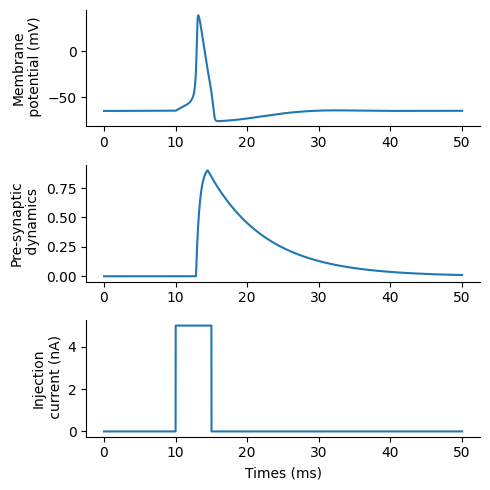
\includegraphics[scale=0.8, max width=\linewidth]{./fig/synapse-model/kinetic-synapse/cell008.png}
	\caption{cell008.png}
	\label{cell008.png}
\end{figure}

% \section{シナプス入力の重みづけ
}


ここまでは, シナプス前細胞と後細胞がそれぞれ1つずつである場合について考えていたが, 実際には多数の細胞がネットワークを作っている.また, それぞれの入力は均等ではなく, 異なるシナプス強度 (Synaptic strength)を持つ.この場合のシナプス入力の計算について述べておく.



シナプス前細胞が$N_{\text{pre}}$個, シナプス後細胞が$N_{\text{post}}$個あるとする.このとき\textbf{シナプス前過程に注目した}\index{しなぷすまえかていにちゅうもくした@シナプス前過程に注目した}シナプス動態を$\boldsymbol{s_{\text{syn}}}\in \mathbb{R}^{N_{\text{pre}}}$, シナプス後細胞の入力電流を$\boldsymbol{I_{\text{syn}}}\in \mathbb{R}^{N_{\text{post}}}$, シナプス結合強度の行列を$W\in \mathbb{R}^{N_{\text{post}} \times N_{\text{pre}}}$とすると, Current-basedの場合は





\begin{equation}

\boldsymbol{I_{\text{syn}}}(t)=W \boldsymbol{s_{\text{syn}}}  

\end{equation}





となる.ただし, シナプス強度にシナプス効率が含まれるとした. また, Conductance-basedの場合はシナプス後細胞の膜電位を$\boldsymbol{V}_{m}\in \mathbb{R}^{N_{\text{post}}}$として, 





\begin{equation}

\boldsymbol{I_{\text{syn}}}(t)=\left(V_{\text{syn}}-\boldsymbol{V}_{m}(t)\right)\odot W \boldsymbol{s_{\text{syn}}}

\end{equation}





となる.ただし, $\odot$はHadamard積である.



これらの式は順序を入れ替えることも可能である.シナプス前細胞でスパイクが生じたことを表すベクトルを$\boldsymbol{\delta}_{t,t_{\text{spike}}}\in \mathbb{R}^{N_{\text{pre}}}$とする.ただし, $t_{\text{spike}}$は各ニューロンにおいてスパイクが生じた時刻である. $\boldsymbol{s_{\text{syn}}}$は$\boldsymbol{\delta}_{t,t_{\text{spike}}}$の関数であり, $\boldsymbol{s_{\text{syn}}}(\boldsymbol{\delta}_{t,t_{\text{spike}}})$と表せる.このとき\textbf{シナプス後過程に注目した}\index{しなぷすのちかていにちゅうもくした@シナプス後過程に注目した}シナプス動態を$\boldsymbol{s}^\prime_{\text{syn}}\in \mathbb{R}^{N_{\text{post}}}$とすると, Current-basedの場合は





\begin{equation}

\boldsymbol{I_{\text{syn}}}(t)=\boldsymbol{s}^\prime_{\text{syn}}(W\boldsymbol{\delta}_{t,t_{\text{spike}}})  

\end{equation}





Conductance-basedの場合は





\begin{equation}

\boldsymbol{I_{\text{syn}}}(t)=\left(V_{\text{syn}}-\boldsymbol{V}_{m}(t)\right)\odot \boldsymbol{s}^\prime_{\text{syn}}(W\boldsymbol{\delta}_{t,t_{\text{spike}}})

\end{equation}





と表すことができる.



シナプス動態を前過程か後過程のどちらに注目したものとするかは, 実装によって様々である.シナプス入力の計算における中間の値を学習に用いるということもあるため, 単なる計算量の観点だけではどちらを選ぶかは決めることができない (計算量だけならシナプス変数に先に重み行列をかけた方がよい場合が多い).実装の中で異なってくるのは計算順序と保持するベクトルの要素数である. 同じ実装の中で2つとも用いる場合もあるので注意してほしい.

 % ok
% \section{動的シナプス}

シナプス前活動に応じて\textbf{シナプス伝達効率}\index{しなぷすでんたつこうりつ@シナプス伝達効率} (synaptic efficacy)が動的に変化する性質を\textbf{短期的シナプス可塑性}\index{たんきてきしなぷすかそせい@短期的シナプス可塑性} (Short-term synaptic plasticity)といい,このような性質を持つシナプスを\textbf{動的シナプス}\index{どうてきしなぷす@動的シナプス} (dynamical synapses)と呼ぶ.シナプス伝達効率が減衰する現象を短期抑圧 (short-term depression; STD),増強する現象を短期促通(short-term facilitation; STF)という.さらにそれぞれに対応するシナプスを減衰シナプス,増強シナプスという.

ここでは\citep{Mongillo2008-kk}および\citep{Orhan2019-rq}で用いられている定式化を使用する.


\begin{gathered}
\frac{\mathrm{d} x(t)}{\mathrm{d} t}=\frac{1-x(t)}{\tau_{x}}-u(t) x(t) r(t) \Delta t \\
\frac{\mathrm{d} u(t)}{\mathrm{d} t}=\frac{U-u(t)}{\tau_{u}}+U(1-u(t)) r(t) \Delta t
\end{gathered}


ただし,定数は以下のようにする.
\begin{itemize}
\item STSP neurotransmitter time constant: $\tau_x$ 200 ms/1,500 ms (facilitating/depressing)
\item STSP neurotransmitter utilization: $\tau_u$ 1,500 ms/200 ms (facilitating/depressing)
\item STSP neurotransmitter increment: $U$ 0.15/0.45 (facilitating/depressing)
\item Time step (training and testing): $\Delta t$ 10ms
\end{itemize}

\begin{itemize}
\item $x$: the fraction of available neurotransmitter
\item $u$: the neurotransmitter utilization
\end{itemize}
\lstinputlisting[language=julia]{./text/synapse-model/dynamical-synapses/001.jl}
\lstinputlisting[language=julia]{./text/synapse-model/dynamical-synapses/002.jl}
\lstinputlisting[language=julia]{./text/synapse-model/dynamical-synapses/003.jl}
\lstinputlisting[language=julia]{./text/synapse-model/dynamical-synapses/004.jl}
\lstinputlisting[language=julia]{./text/synapse-model/dynamical-synapses/005.jl}
\begin{figure}[ht]
	\centering
	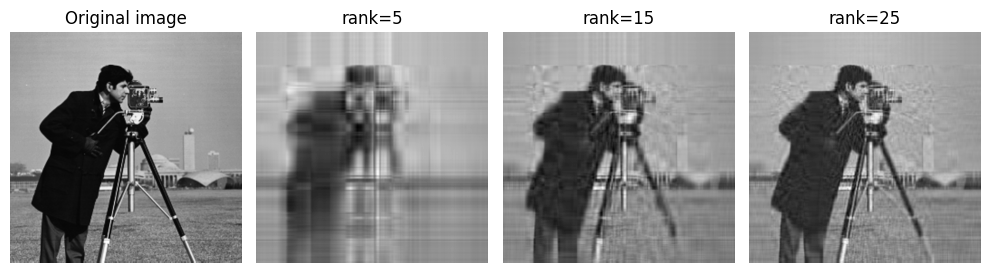
\includegraphics[scale=0.8, max width=\linewidth]{./fig/solve-credit-assignment-problem/linear-network-learning-dynamics/cell005.png}
	\caption{cell005.png}
	\label{cell005.png}
\end{figure}


\chapter{神経回路網の演算処理}
% \section{ゲイン調節と四則演算}
\citep{Goldwyn2018-ug}を実装.神経演算 (neuronal arithmetic; \citep{Angus_Silver2010-fd})のモデル.
\begin{lstlisting}[language=julia]
using Base: @kwdef
using Parameters: @unpack # or using UnPack
using PyPlot, ProgressMeter, Distributions
rc("axes.spines", top=false, right=false)
\end{lstlisting}
\begin{lstlisting}[language=julia]
@kwdef struct HHIAParameter{FT}
    Cm::FT  = 1 # 膜容量(uF/cm^2)
    gNa::FT = 37; gK::FT = 45; gA::FT = 20; gL::FT = 1 # Na, K, Kₐ, leakの最大コンダクタンス(mS/cm^2)
    ENa::FT = 55; EK::FT = -80; EL::FT = -70 #Na, K, leakの平衡電位(mV)
    gExc::FT = 0.5; gInh::FT = 1
    VExc::FT = 0;   VInh::FT = -85
    βExc::FT = 0.2; βInh::FT = 0.18
    tr::FT = 0.5;   td::FT = 8 # ms
    γ1::FT = 1/td;  γ2::FT = 1/tr - 1/td
    v0::FT = -20 # mV
end

@kwdef mutable struct HHIA{FT}
    param::HHIAParameter = HHIAParameter{FT}()
    N::Int
    v::Vector{FT} = fill(-70, N); r::Vector{FT} = zeros(N)
    n::Vector{FT} = fill(1/(1 + exp(-(-70 + 32)/8)), N)
    a::Vector{FT} = fill(1/(1 + exp(-(-70 + 50)/20)), N)
    b::Vector{FT} = fill(1/(1 + exp((-70 + 70)/6)), N)
    sExc::Vector{FT} = zeros(N); sInh::Vector{FT} = zeros(N)
end
\end{lstlisting}
\begin{lstlisting}[language=julia]
function update!(variable::HHIA, param::HHIAParameter, spikesExc::Vector, spikesInh::Vector, dt)
    @unpack N, v, n, a, b, r, sExc, sInh = variable
    @unpack Cm, gNa, gK, gL, gA, ENa, EK, EL, gExc, gInh, VExc, VInh, βExc, βInh, γ1, γ2, v0 = param
    @inbounds for i = 1:N
        m, h = 1 / (1 + exp(-(v[i]+30)/15)), 1 - n[i]
        
        n[i] += dt * 0.75(1/(1 + exp(-0.125(v[i] + 32))) - n[i]) / (1 + 100 / (1 + exp((v[i] + 80)/26)))
        a[i] += dt * 0.5(1/(1 + exp(-0.05(v[i] + 50))) - a[i])
        b[i] += dt * (1.0/(1 + exp((v[i] + 70)/6)) - b[i]) / 150
        
        sExc[i] += -sExc[i] * βExc*dt + spikesExc[i]
        sInh[i] += -sInh[i] * βInh*dt + spikesInh[i]
        IExc = gExc * sExc[i] * (v[i] - VExc) 
        IInh = gInh * sInh[i] * (v[i] - VInh)

        IL = gL * (v[i] - EL)
        IK = gK * n[i]^4 * (v[i] - EK)
        IA = gA * a[i]^3 * b[i] * (v[i] - EK)
        INa = gNa * m^3 * h * (v[i] - ENa)
        
        v[i] += dt/Cm * -(IL + IK + IA + INa + IExc + IInh)
        r[i] += dt * (γ2 * (1.0 - r[i])/(1.0 + exp(-v[i] + v0)) - r[i] * γ1)
    end
end
\end{lstlisting}
\begin{lstlisting}[language=julia]
function GammaSpike(T, dt, n_neurons, fr, k)
    nt = Int(T/dt) # number of timesteps
    θ = 1/(k*(fr*dt*1e-3)) # fr = 1/(k*θ)

    isi = rand(Gamma(k, θ), Int(round(nt*1.5/fr)), n_neurons)
    spike_time = cumsum(isi, dims=1) # ISIを累積
    spike_time[spike_time .> nt - 1] .= 1 # ntを超える場合を1に
    spike_time = round.(Int, spike_time) # float to int
    spikes = zeros(Bool, nt, n_neurons) # スパイク記録変数

    for i=1:n_neurons    
        spikes[spike_time[:, i], i] .= 1
    end

    spikes[1] = 0 # (spike_time=1)の発火を削除
    return spikes
end
\end{lstlisting}
\begin{lstlisting}[language=julia]
function FIcurve(neurons, spikesExc, spikesInh, T=5000, dt=0.01)
    nt = Int(T/dt) # number of timesteps
    varr = zeros(Float32, nt,  neurons.N)
    
    @showprogress for t = 1:nt
        update!(neurons, neurons.param, spikesExc[t, :], spikesInh[t, :], dt)
        varr[t, :] = neurons.v
    end
    
    spike = (varr[1:nt-1, :] .< 0) .& (varr[2:nt, :] .> 0)
    output_spikes = sum(spike, dims=1) / T*1e3
    input_spikes = sum(spikesExc, dims=1) / T*1e3
    return input_spikes, output_spikes
end
\end{lstlisting}
\begin{lstlisting}[language=julia]
T, dt = 50000, 5e-2 # ms
nt = Int(T/dt)
N = 100
maxfrExc = 80; frInh = [0, 50]; 
\end{lstlisting}
\begin{lstlisting}[language=julia]
function HHIAFIcurve_multi(gA, T, dt, N, maxfrExc, frInh)
    nInh = size(frInh)[1]
    input_spikes_arr, output_spikes_arr = zeros(nInh, N), zeros(nInh, N)
    nt = Int(T/dt) # number of timesteps
    frExc = rand(N) * maxfrExc
    spikesExc = zeros(Int, nt, N)
    for j = 1:N
        spikesExc[:, j] = rand(nt) .< frExc[j]*dt*1e-3
    end
    for i=1:nInh
        spikesInh = (frInh[i] == 0) ? zeros(Int, nt, N) : GammaSpike(T, dt, N, frInh[i], 12)    
        neurons = HHIA{Float32}(N=N, param=HHIAParameter{Float32}(gA=gA)) # modelの定義
        input_spikes_arr[i, :], output_spikes_arr[i, :] = FIcurve(neurons, spikesExc, spikesInh, T, dt)
    end
    return input_spikes_arr, output_spikes_arr
end
\end{lstlisting}
\begin{lstlisting}[language=julia]
input_spikes1, output_spikes1 = HHIAFIcurve_multi(20, T, dt, N, maxfrExc, frInh);
input_spikes2, output_spikes2 = HHIAFIcurve_multi(40, T, dt, N, maxfrExc, frInh);
\end{lstlisting}
\begin{lstlisting}[language=julia]
figure(figsize=(10, 4))
subplot(1,3,1); title(L"Divisive inhibition (g$_A=20$)")
scatter(input_spikes1[1, :], output_spikes1[1, :], facecolor="white", edgecolors="tab:red", label="no inhibition")
scatter(input_spikes1[2, :], output_spikes1[2, :], alpha=0.5, color="tab:red", label="inhibition")
xlim(0, ); ylim(0, ); xlabel("Input spikes/s"); ylabel("Output spikes/s"); legend()
subplot(1,3,2); title(L"Subtractive inhibition (g$_A=40$)")
scatter(input_spikes2[1, :], output_spikes2[1, :], facecolor="white", edgecolors="tab:blue", label="no inhibition")
scatter(input_spikes2[2, :], output_spikes2[2, :], alpha=0.5, color="tab:blue", label="inhibition")
xlim(0, ); ylim(0, ); xlabel("Input spikes/s"); ylabel("Output spikes/s"); legend()
subplot(1,3,3);
scatter(output_spikes1[1, :], output_spikes1[2, :], alpha=0.5, color="tab:red", label=L"g$_A=20$")
scatter(output_spikes2[1, :], output_spikes2[2, :], alpha=0.5, color="tab:blue", label=L"g$_A=40$")
xlim(0, ); ylim(0, ); xlabel("Output spike/s\n No Inhibition"); ylabel("Output spike/s\n with Inhibition"); legend()
tight_layout()
\end{lstlisting}
\begin{figure}[ht]
	\centering
	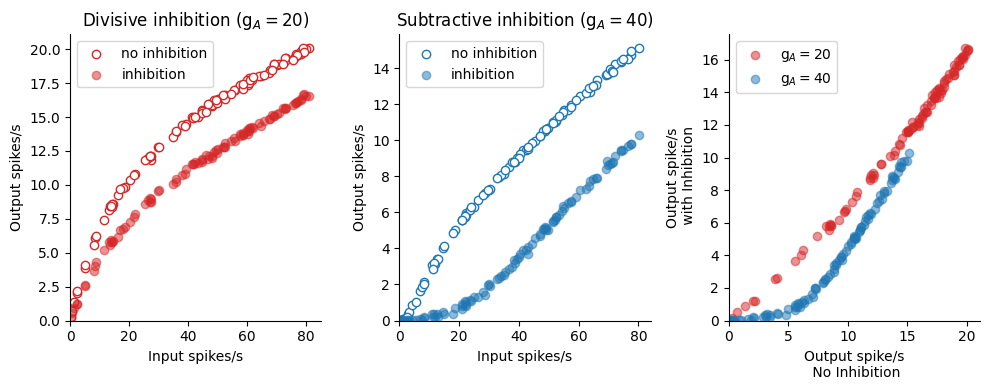
\includegraphics[scale=0.8, max width=\linewidth]{./fig/neuronal-computation/neuronal-arithmetic/cell009.png}
	\caption{cell009.png}
	\label{cell009.png}
\end{figure}
 % ok

\chapter{局所学習則}
% \section{Hebb則と教師なし学習}
\subsection{Hebb則}
神経回路はどのようにして自己組織化するのだろうか.1940年代にカナダの心理学者Donald O. Hebbにより著書"The Organization of Behavior"\cite{Hebb1949-iv} で提案された学習則は「細胞Aが反復的または持続的に細胞Bの発火に関与すると,細胞Aが細胞Bを発火させる効率が向上するような成長過程または代謝変化が一方または両方の細胞に起こる」というものであった.すなわち,発火に時間的相関のある細胞間のシナプス結合を強化するという学習則である.これを\textbf{Hebbの学習則 (Hebbian learning rule)} あるいは\textbf{Hebb則(Hebb's rule)} という.Hebb則は (Hebb自身ではなく) Shatzにより"cells that fire together wire together" (共に活動する細胞は共に結合する)と韻を踏みながら短く言い換えられている \cite{Shatz1992-he}.

\subsubsection{Hebb則の導出}
数式でHebb則を表してみよう.$n$個のシナプス前細胞と$m$個の後細胞の発火率をそれぞれ$\mathbf{x}\in \mathbb{R}^n, \mathbf{y}\in \mathbb{R}^m$ とする.前細胞と後細胞間のシナプス結合強度を表す行列を$\mathbf{W}\in \mathbb{R}^{m\times n}$とし,$\mathbf{y}=\mathbf{W}\mathbf{x}$が成り立つとする.このようなモデルを線形ニューロンモデル (Linear neuron model) という.このとき,Hebb則は


\begin{equation}
\tau\frac{d\mathbf{W}}{dt}=\phi(\mathbf{y})\varphi(\mathbf{x})^\top
\end{equation}


として表される.ただし,$\tau$は時定数であり,$\eta:=1/\tau$ は\textbf{学習率 (learning rate)} と呼ばれる学習の速さを決定するパラメータとなる.$\varphi(\cdot)$および$\phi(\cdot)$は,それぞれシナプス前細胞および後細胞の活動量に応じて重みの変化量を決定する関数である.ただし,$\varphi(\cdot), \phi(\cdot)$は基本的に恒等関数に設定される場合が多い.この場合,Hebb則は$
\tau\dfrac{d\mathbf{W}}{dt}=\mathbf{y}\mathbf{x}^\top=(\text{post})\cdot (\text{pre})^\top
$と簡潔に表現される.

このHebb則は数学的に導出されたものではないが,特定の目的関数を神経活動及び重みを変化させて最適化するようなネットワークを構築すれば自然に出現する.このようなネットワークを\textbf{エネルギーベースモデル (energy-based models)} といい,次章で扱う.エネルギーベースモデルでは,先にエネルギー関数 (あるいはコスト関数) $\mathcal{E}$ を定義し,その目的関数を最小化するような神経活動 $\mathbf{z}$ および重み行列 $\mathbf{W}$ のダイナミクスをそれぞれ,


\begin{equation}
\frac{d \mathbf{z}}{dt}\propto-\frac{\partial \mathcal{E}}{\partial \mathbf{z}},\ \frac{d \mathbf{W}}{dt}\propto-\frac{\partial \mathcal{E}}{\partial \mathbf{W}}
\end{equation}


として導出する.この手順の逆を行う,すなわち先に神経細胞の活動ダイナミクスを定義し,神経活動で積分することで神経回路のエネルギー関数$\mathcal{E}$を導出し,さらに $\mathcal{E}$ を重み行列で微分することでHebb則が導出できる \cite{Isomura2020-sn}.Hebb則の導出を連続時間線形ニューロンモデル $\dfrac{d\mathbf{y}}{dt}=\mathbf{W}\mathbf{x}$ を例にして考えよう.ここで$\dfrac{\partial\mathcal{E}}{\partial\mathbf{y}}:=-\dfrac{d\mathbf{y}}{dt}$となるようなエネルギー関数 $\mathcal{E}(\mathbf{x}, \mathbf{y}, \mathbf{W})$を仮定すると,


\begin{equation}
\mathcal{E}(\mathbf{x}, \mathbf{y}, \mathbf{W})=-\int \mathbf{W}\mathbf{x}\ d\mathbf{y}=-\mathbf{y}^\top \mathbf{W}\mathbf{x} \in \mathbb{R}
\end{equation}


となる.これをさらに$\mathbf{W}$で微分すると,


\begin{equation}
\dfrac{\partial\mathcal{E}}{\partial\mathbf{W}}=-\mathbf{y}\mathbf{x}^\top\Rightarrow
\frac{d\mathbf{W}}{dt}=-\dfrac{\partial\mathcal{E}}{\partial\mathbf{W}}=\mathbf{y}\mathbf{x}^\top
\end{equation}


となり,Hebb則が導出できる (簡単のため時定数は1とした).
\subsection{Hebb則の安定化とLTP/LTD}
\subsubsection{BCM則}
Hebb則には問題点があり,シナプス結合強度が際限なく増大するか,0に近づくこととなってしまう.これを数式で確認しておこう.前細胞と後細胞がそれぞれ1つの場合を考える.2細胞間の結合強度を$w\ (>0)$ とし,$y=wx$が成り立つとすると,Hebb則は$\dfrac{dw}{dt}=\eta yx=\eta x^2w$となる.この場合,$\eta x^2>1$ なら $\lim_{t\to\infty} w= \infty$, $\eta x^2<1$ なら $\lim_{t\to\infty} w= 0$ となる.当然,生理的にシナプス結合強度が無限大となることはあり得ないが,不安定なほど大きくなってしまう可能性があることに違いはない.このため,Hebb則を安定化させるための修正が必要とされた.

Cooper, Liberman, Ojaらにより頭文字をとって\textbf{CLO則} (CLO rule) が提案された \cite{Cooper1979-wz}.その後,Bienenstock, Cooper, Munroらにより提案された学習則は同様に頭文字をとって\textbf{BCM則} (BCM rule) と呼ばれている\cite{Bienenstock1982-km} \cite{Cooper2012-ec}.

$\mathbf{x}\in \mathbb{R}^d, \mathbf{w}\in \mathbb{R}^d, y\in \mathbb{R}$とし,単一の出力$y = \mathbf{w}^\top \mathbf{x}=\mathbf{x}^\top \mathbf{w}$を持つ線形ニューロンを仮定する.重みの更新則は次のようにする.


\begin{equation}
\frac{d\mathbf{w}}{dt} = \eta_w \mathbf{x} \phi(y, \theta_m)
\end{equation}


ここで関数$\phi$は$\phi(y, \theta_m)=y(y-\theta_m)$などとする.また$\theta_m:=\mathbb{E}[y^2]$は閾値を決定するパラメータ,\textbf{修正閾値(modification threshold)} であり,


\begin{equation}
\frac{d\theta_m}{dt} = \eta_{\theta} \left(y^2-\theta_m\right)
\end{equation}


として更新される.

ToDo: 詳細
\lstinputlisting[language=julia]{./text/local-learning-rule/pca-hebbian-learning/002.jl}
\lstinputlisting[language=julia]{./text/local-learning-rule/pca-hebbian-learning/003.jl}
\lstinputlisting[language=julia]{./text/local-learning-rule/pca-hebbian-learning/004.jl}
\begin{figure}[ht]
	\centering
	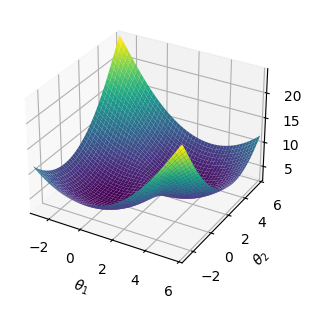
\includegraphics[scale=0.8, max width=\linewidth]{./fig/bayesian-brain/mcmc/cell004.png}
	\caption{cell004.png}
	\label{cell004.png}
\end{figure}
\subsubsection{Hebb則の生理的機序}
ここでHebb則およびBCM則の生理的基盤について触れておこう.
LTPの実験的発見 \cite{Bliss1973-vj} \cite{Dudek1992-nz}

ToDo:実験的発見のsurvey
\subsubsection{Oja則}
Hebb則を安定化させる別のアプローチとして,結合強度を正規化するという手法が考えられる.BCM則と同様に$\mathbf{x}\in \mathbb{R}^d, \mathbf{w}\in \mathbb{R}^d, y\in \mathbb{R}$とし,単一の出力$y = \mathbf{w}^\top \mathbf{x}=\mathbf{x}^\top \mathbf{w}$を持つ線形ニューロンを仮定する.$\eta$を学習率とすると,$\mathbf{w}\leftarrow\dfrac{\mathbf{w}+\eta \mathbf{x}y}{\|\mathbf{w}+\eta \mathbf{x}y\|}$とすれば正規化できる.ここで,$f(\eta):=\dfrac{\mathbf{w}+\eta \mathbf{x}y}{\|\mathbf{w}+\eta \mathbf{x}y\|}$とし,$\eta=0$においてTaylor展開を行うと,


\begin{align}
f(\eta)&\approx f(0) + \eta \left.\frac{df(\eta^*)}{d\eta^*}\right|_{\eta^*=0} + \mathcal{O}(\eta^2)\\
&=\frac{\mathbf{w}}{\|\mathbf{w}\|} + \eta \left(\frac{\mathbf{x}y}{\|\mathbf{w}\|}-\frac{y^2\mathbf{w}}{\|\mathbf{w}\|^3}\right)+ \mathcal{O}(\eta^2)
\end{align}


ここで$\|\mathbf{w}\|=1$として,1次近似すれば$f(\eta)\approx \mathbf{w} + \eta \left(\mathbf{x}y-y^2 \mathbf{w}\right)$となる.重みの変化が連続的であるとすると,


\begin{equation}
\frac{d\mathbf{w}}{dt} = \eta \left(\mathbf{x}y-y^2 \mathbf{w}\right)
\end{equation}


として重みの更新則が得られる.これを\textbf{Oja則 (Oja's rule)} と呼ぶ \cite{Oja1982-yd}.こうして得られた学習則において$\|\mathbf{w}\|\to 1$となることを確認しよう.


\begin{equation}
\frac{d\|\mathbf{w}\|^2}{dt}=2\mathbf{w}^\top\frac{d\mathbf{w}}{dt}= 2\eta y^2\left(1-\|\mathbf{w}\|^2\right)
\end{equation}


より,$\dfrac{d\|\mathbf{w}\|^2}{dt}=0$のとき,$\|\mathbf{w}\|= 1$となる.
\subsubsection{恒常的可塑性}
Oja則は更新時の即時的な正規化から導出されたものであるが,恒常的可塑性 (synaptic scaling)により安定化しているという説がある\cite{Turrigiano2008-lm}\cite{Yee2017-fb}.しかし,この過程は遅すぎるため,Hebb則の不安定化を安定化するに至らない\cite{Zenke2017-el}

ToDo:恒常的可塑性の詳細

Johansen, Joshua P., Lorenzo Diaz-Mataix, Hiroki Hamanaka, Takaaki Ozawa, Edgar Ycu, Jenny Koivumaa, Ashwani Kumar, et al. 2014. “Hebbian and Neuromodulatory Mechanisms Interact to Trigger Associative Memory Formation.” Proceedings of the National Academy of Sciences 111 (51): E5584–92.
\subsection{Hebb則と主成分分析}
Oja則を用いることで\textbf{主成分分析(Principal component analysis; PCA)} という処理をニューラルネットワークにおいて実現できる.主成分分析とは-

ToDo:主成分分析の説明
\lstinputlisting[language=julia]{./text/local-learning-rule/pca-hebbian-learning/009.jl}
\lstinputlisting[language=julia]{./text/local-learning-rule/pca-hebbian-learning/010.jl}
\lstinputlisting[language=julia]{./text/local-learning-rule/pca-hebbian-learning/011.jl}
\begin{figure}[ht]
	\centering
	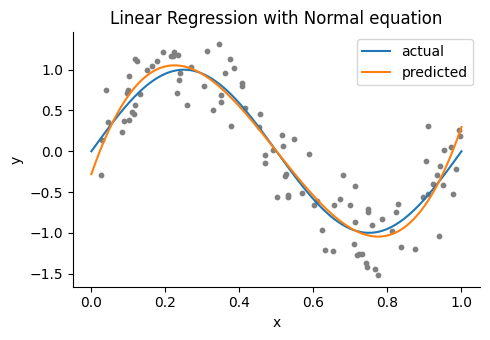
\includegraphics[scale=0.8, max width=\linewidth]{./fig/introduction/linear-regression/cell011.png}
	\caption{cell011.png}
	\label{cell011.png}
\end{figure}
\subsubsection{Oja則によるPCAの実行}
ここでOja則が主成分分析を実行できることを示す.重みの変化量の期待値を取る.


\begin{align}
\frac{d\mathbf{w}}{dt} &= \eta \left(\mathbf{x}y - y^2 \mathbf{w}\right)=\eta \left(\mathbf{x}\mathbf{x}^\top \mathbf{w} - \left[\mathbf{w}^\top \mathbf{x}\mathbf{x}^\top \mathbf{w}\right] \mathbf{w}\right)\\
\mathbb{E}\left[\frac{d\mathbf{w}}{dt}\right] &= \eta \left(\mathbf{C} \mathbf{w} - \left[\mathbf{w}^\top \mathbf{C} \mathbf{w}\right] \mathbf{w}\right)
\end{align}


$\mathbf{C}:=\mathbb{E}[\mathbf{x}\mathbf{x}^\top]\in \mathbb{R}^{d\times d}$とする.$\mathbf{x}$の平均が0の場合,$\mathbf{C}$は分散共分散行列である.$\mathbb{E}\left[\dfrac{d\mathbf{w}}{dt}\right]=0$となる$\mathbf{w}$が収束する固定点(fixed point)では次の式が成り立つ.


\begin{equation}
\mathbf{C}\mathbf{w} = \lambda \mathbf{w}
\end{equation}


これは固有値問題であり,$\lambda:=\mathbf{w}^\top \mathbf{C} \mathbf{w}$は固有値,$\mathbf{w}$は固有ベクトル(eigen vector)になる.

ここでサンプルサイズを$n$とし,$\mathbf{X} \in \mathbb{R}^{d\times n}, \mathbf{y}=\mathbf{X}^\top\mathbf{w} \in \mathbb{R}^n$とする.標本平均で近似して$\mathbf{C}\simeq \mathbf{X}\mathbf{X}^\top$とする.この場合,


\begin{align}
\mathbb{E}\left[\frac{d\mathbf{w}}{dt}\right] &\simeq \eta \left(\mathbf{X}\mathbf{X}^\top \mathbf{w} - \left[\mathbf{w}^\top \mathbf{X}\mathbf{X}^\top \mathbf{w}\right] \mathbf{w}\right)\\
&=\eta \left(\mathbf{X}\mathbf{y} - \left[\mathbf{y}^\top\mathbf{y}\right] \mathbf{w}\right)
\end{align}


となる.
\lstinputlisting[language=julia]{./text/local-learning-rule/pca-hebbian-learning/013.jl}
\lstinputlisting[language=julia]{./text/local-learning-rule/pca-hebbian-learning/014.jl}
\begin{figure}[ht]
	\centering
	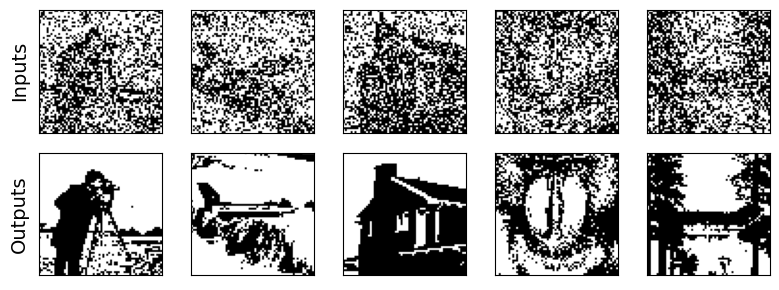
\includegraphics[scale=0.8, max width=\linewidth]{./fig/energy-based-model/hopfield-model/cell014.png}
	\caption{cell014.png}
	\label{cell014.png}
\end{figure}
後のためにOja則においてネットワークが$q$個の複数出力を持つ場合を考えよう.重み行列を$\mathbf{W} \in \mathbb{R}^{q\times d}$, 出力を$\mathbf{y}=\mathbf{W}\mathbf{x} \in \mathbb{R}^{q}, \mathbf{Y}=\mathbf{W}\mathbf{X} \in \mathbb{R}^{q\times n}$とする.この場合の更新則は


\begin{equation}
\frac{d\mathbf{W}}{dt} = \eta \left(\mathbf{y}\mathbf{x}^\top - \mathrm{Diag}\left[\mathbf{y}\mathbf{y}^\top\right] \mathbf{W}\right)
\end{equation}


となる.ただし,$\mathrm{Diag}(\cdot)$は行列の対角成分からなる対角行列を生み出す作用素である.
\subsubsection{Sanger則}
Oja則に複数の出力を持たせた場合であっても,出力が直交しないため,PCAの第1主成分しか求めることができない.\textbf{Sanger則 (Sanger's rule)},あるいは\textbf{一般化Hebb則 (generalized Hebbian algorithm; GHA)} は,Oja則に\textbf{Gram–Schmidtの正規直交化法(Gram–Schmidt orthonormalization)} を組み合わせた学習則であり,次式で表される.


\begin{equation}
\frac{d\mathbf{W}}{dt} = \eta \left(\mathbf{y}\mathbf{x}^\top - \mathrm{LT}\left[\mathbf{y}\mathbf{y}^\top\right] \mathbf{W}\right)
\end{equation}


$\mathrm{LT}(\cdot)$は行列の対角成分より上側の要素を0にした下三角行列(lower triangular matrix)を作り出す作用素である.Sanger則を用いればPCAの第2主成分以降も求めることができる.
\lstinputlisting[language=julia]{./text/local-learning-rule/pca-hebbian-learning/017.jl}
\lstinputlisting[language=julia]{./text/local-learning-rule/pca-hebbian-learning/018.jl}
\begin{figure}[ht]
	\centering
	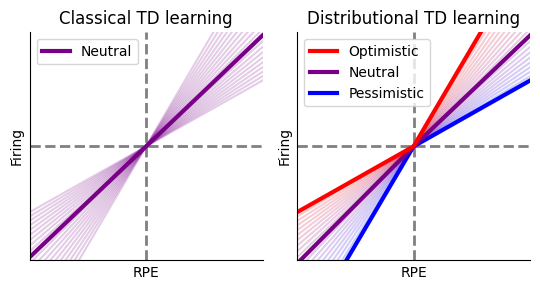
\includegraphics[scale=0.8, max width=\linewidth]{./fig/bayesian-brain/quantile-expectile-regression/cell018.png}
	\caption{cell018.png}
	\label{cell018.png}
\end{figure}
Oja則,Sanger則をまとめて一つの関数にしておこう.\jl{identity()}は恒等関数である.
\lstinputlisting[language=julia]{./text/local-learning-rule/pca-hebbian-learning/020.jl}
\subsection{非線形Hebb学習}
出力$\mathbf{y}$に非線形関数$g(\cdot)$を適用し,$\mathbf{y}\to g(\mathbf{y})$として置き換えることで非線形Hebb学習となる\cite{Oja1997-hr}\cite{Brito2016-mx}. 関数\jl{HebbianPCA}の\jl{func}引数に非線形関数を渡すことで実現できる.

ToDo: 詳細
\subsubsection{非負主成分分析によるグリッドパターンの創発}
内側嗅内皮質(MEC)にある\textbf{グリッド細胞 (grid cells)} は六角形格子状の発火パターンにより自己位置等を符号化するのに貢献している.この発火パターンを生み出すモデルは多数あるが,\textbf{場所細胞(place cells)} の発火パターンを\textbf{非負主成分分析(nonnegative principal component analysis)} で次元削減するとグリッド細胞のパターンが生まれるというモデルがある \cite{Dordek2016-ff}.非線形Hebb学習を用いてこのモデルを実装しよう.なお,同様のことは\textbf{非負値行列因子分解 (NMF: nonnegative matrix factorization)} でも可能である.
\paragraph{場所細胞の発火パターン}
まず,訓練データとなる場所細胞の発火パターンを人工的に作成する.場所細胞の発火パターンは\textbf{Difference of Gaussians (DoG)} で近似する.DoGは大きさの異なる2つのガウス関数の差分を取った関数であり,画像に適応すればband-passフィルタとして機能する.また,DoGは網膜神経節細胞等の受容野のON中心OFF周辺型受容野のモデルとしても用いられる.受容野中央では活動が大きく,その周辺では活動が抑制される,という特性を持つ.2次元のガウス関数とDoG関数を実装する.
\lstinputlisting[language=julia]{./text/local-learning-rule/pca-hebbian-learning/024.jl}
モデルのパラメータを設定する.
\lstinputlisting[language=julia]{./text/local-learning-rule/pca-hebbian-learning/026.jl}
先にガウス関数とDoG関数がどのような見た目になるか確認しよう.
\lstinputlisting[language=julia]{./text/local-learning-rule/pca-hebbian-learning/028.jl}
\lstinputlisting[language=julia]{./text/local-learning-rule/pca-hebbian-learning/029.jl}
\begin{figure}[ht]
	\centering
	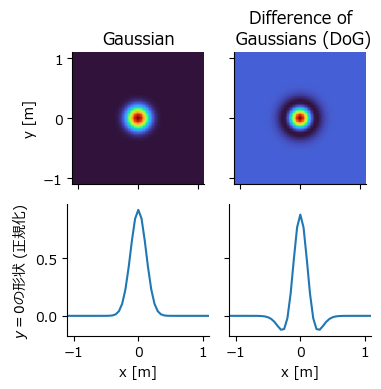
\includegraphics[scale=0.8, max width=\linewidth]{./fig/local-learning-rule/pca-hebbian-learning/cell029.png}
	\caption{cell029.png}
	\label{cell029.png}
\end{figure}
場所細胞の活動パターンを生み出す.それぞれの場所受容野の中心は空間を均等に覆うように作成する (一様分布で生み出してもよい).
\lstinputlisting[language=julia]{./text/local-learning-rule/pca-hebbian-learning/031.jl}
線形PCAの場合
\lstinputlisting[language=julia]{./text/local-learning-rule/pca-hebbian-learning/033.jl}
\lstinputlisting[language=julia]{./text/local-learning-rule/pca-hebbian-learning/034.jl}
\begin{figure}[ht]
	\centering
	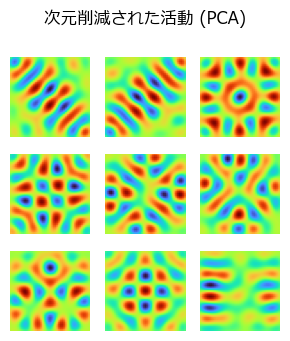
\includegraphics[scale=0.8, max width=\linewidth]{./fig/local-learning-rule/pca-hebbian-learning/cell034.png}
	\caption{cell034.png}
	\label{cell034.png}
\end{figure}
自己相関マップ(autocorrelation map)を確認する.

ToDo: 相関の計算の説明
\lstinputlisting[language=julia]{./text/local-learning-rule/pca-hebbian-learning/036.jl}
\lstinputlisting[language=julia]{./text/local-learning-rule/pca-hebbian-learning/037.jl}
\lstinputlisting[language=julia]{./text/local-learning-rule/pca-hebbian-learning/038.jl}
\begin{figure}[ht]
	\centering
	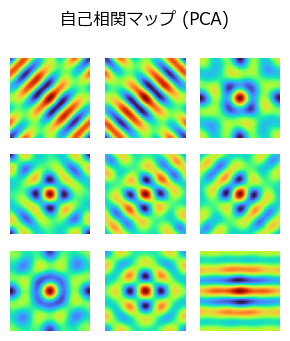
\includegraphics[scale=0.8, max width=\linewidth]{./fig/local-learning-rule/pca-hebbian-learning/cell038.png}
	\caption{cell038.png}
	\label{cell038.png}
\end{figure}
非負PCAの場合
\lstinputlisting[language=julia]{./text/local-learning-rule/pca-hebbian-learning/040.jl}
\lstinputlisting[language=julia]{./text/local-learning-rule/pca-hebbian-learning/041.jl}
\lstinputlisting[language=julia]{./text/local-learning-rule/pca-hebbian-learning/042.jl}
\begin{figure}[ht]
	\centering
	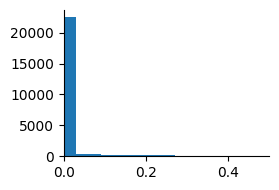
\includegraphics[scale=0.8, max width=\linewidth]{./fig/energy-based-model/sparse-coding/cell042.png}
	\caption{cell042.png}
	\label{cell042.png}
\end{figure}
\lstinputlisting[language=julia]{./text/local-learning-rule/pca-hebbian-learning/043.jl}
\lstinputlisting[language=julia]{./text/local-learning-rule/pca-hebbian-learning/044.jl}
\begin{figure}[ht]
	\centering
	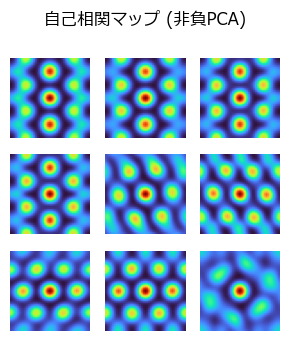
\includegraphics[scale=0.8, max width=\linewidth]{./fig/local-learning-rule/pca-hebbian-learning/cell044.png}
	\caption{cell044.png}
	\label{cell044.png}
\end{figure}
Place cellの受容野をDoGに設定したが,これが無いと格子状の受容野は出現しない.path integrationをRNNで実行する場合も同様.一方で,DoGは場所細胞の受容野としては不適切である.

No Free Lunch from Deep Learning in Neuroscience: A Case Study through Models of the Entorhinal-Hippocampal Circuit 
\url{https://openreview.net/forum?id=mxi1xKzNFrb}

ToDo: 他のgrid cellsのモデルについて
 % ok2
% \section{記号の表記
}


本書では次のような記号表記を用いる.

\begin{itemize}
\item 実数全体を$\mathbb{R}$, 複素数全体は$\mathbb{C}$と表記する.

\item スカラーは小文字・斜体で $x$ のように表記する.

\item ベクトルは小文字・立体・太字で $\mathbf{x}$ のように表記し,列ベクトル (縦ベクトル) として扱う.

\item 行列は大文字・立体・太字で $\mathbf{X}$ のように表記する.

\item $n\times 1$の実ベクトルの集合を $\mathbb{R}^n$, $n\times m$ の実行列の集合を $\mathbb{R}^{n\times m}$と表記する.

\item 行列 $\mathbf{X}$ の置換は $\mathbf{X}^\top$と表記する.ベクトルの要素を表す場合は $\mathbf{x} = (x_1, x_2,\cdots, x_n)^\top$のように表記する.

\item 単位行列を $\mathbf{I}$ と表記する.

\item ゼロベクトルは $\mathbf{0}$ , 要素が全て1のベクトルは $\mathbf{1}$ と表記する.  

\item $e$を自然対数の底とし,指数関数を $e^x=\exp(x)$と表記する.また,自然対数を $\ln(x)$と表記する.

\item 定義を$:=$を用いて行う.例えば,$f(x):=2x$は$f(x)$という関数を$2x$として定義するという意味である.

\item 平均 $\mu$, 標準偏差 $\sigma$ の正規分布を $\mathcal{N}(\mu, \sigma^2)$ と表記する.

\end{itemize}


\subsection{変数の命名規則
}


\begin{itemize}
\item \jl{tp1, tm1} : time plus one (t+1), time minus one (t-1)
\end{itemize}


% \section{Slow Feature Analysis (SFA)}
\textbf{Slow Feature Analysis (SFA)}\index{Slow Feature Analysis (SFA)} とは, 複数の時系列データの中から低速に変化する成分 (slow feature) を抽出する教師なし学習のアルゴリズムである (Laurenz Wiskott, Berkes, Franzius, Sprekeler, & Wilbert, 2011; L. Wiskott & Sejnowski, 2002).

潜在変数 $y$ の時間変化の2乗である $\left(\frac{dy}{dt}\right)^2$を最小にするように教師なし学習を行う.初期視覚野の受容野や格子細胞・場所細胞などのモデルに応用がされている (Franzius, Sprekeler, & Wiskott, 2007).

生理学的妥当性についてはいくつかの検討がされている.(Sprekeler, Michaelis, & Wiskott, 2007)ではSTDP則によりSFAが実現できることを報告している.ただし,in vivoにおけるSTDPの存在については近年疑問視されている.これまでのin vitroでの実験は細胞外Ca濃度が高かったために、pre/postのスパイクの時間差でLTD/LTPが生じるという「古典的STDP則」が生じていた可能性があり,細胞外Ca濃度をin vivoの水準まで下げると古典的STDP則は起こらないという報告がある (Inglebert, Aljadeff, Brunel, & Debanne, 2020).古典的な線形Recurrent neural networkでの実装も提案されている ([Lipshutz, Windolf, Golkar, & Chklovskii, 2020](https://arxiv.org/abs/2010.12644)).
\lstinputlisting[language=julia]{./text/local-learning-rule/slow-feature-analysis/001.jl}
\subsection{SFAの前処理}

SFAの前処理として多項式展開(polynomial expandsion)が用いられる ([Berkes & Wiskott, 2005](https://jov.arvojournals.org/article.aspx?articleid=2192836)).Pythonにおいては[sklearn.preprocessing.PolynomialFeatures](https://scikit-learn.org/stable/modules/generated/sklearn.preprocessing.PolynomialFeatures.html)により使用できる.
\lstinputlisting[language=julia]{./text/local-learning-rule/slow-feature-analysis/003.jl}
時間的にずらして時系列データの次元を増やす前処理も行われる.
\lstinputlisting[language=julia]{./text/local-learning-rule/slow-feature-analysis/005.jl}
## データセットの生成
\lstinputlisting[language=julia]{./text/local-learning-rule/slow-feature-analysis/007.jl}
\lstinputlisting[language=julia]{./text/local-learning-rule/slow-feature-analysis/008.jl}
\begin{figure}[ht]
	\centering
	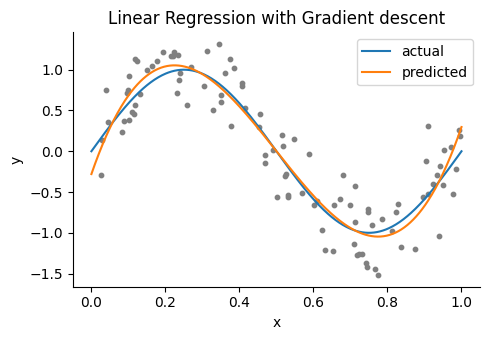
\includegraphics[scale=0.8, max width=\linewidth]{./fig/introduction/linear-regression/cell008.png}
	\caption{cell008.png}
	\label{cell008.png}
\end{figure}
## SFAの実装
\lstinputlisting[language=julia]{./text/local-learning-rule/slow-feature-analysis/010.jl}
## 実行と結果表示
\lstinputlisting[language=julia]{./text/local-learning-rule/slow-feature-analysis/012.jl}
\lstinputlisting[language=julia]{./text/local-learning-rule/slow-feature-analysis/013.jl}
\begin{figure}[ht]
	\centering
	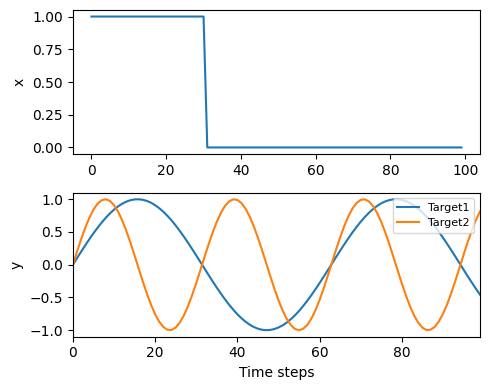
\includegraphics[scale=0.8, max width=\linewidth]{./fig/solve-credit-assignment-problem/bptt/cell013.png}
	\caption{cell013.png}
	\label{cell013.png}
\end{figure}
\subsection{参考文献}
\begin{itemize}
\item \url{https://towardsdatascience.com/a-brief-introduction-to-slow-feature-analysis-18c901bc2a58}
\item \url{https://github.com/flatironinstitute/bio-sfa}
\item \url{https://github.com/fulviadelduca/slow-feature-analysis}
\item [Deep Slow Feature Analysis Network](https://github.com/rulixiang/DSFANet)
\item \url{https://nbviewer.jupyter.org/github/pierrelux/notebooks/blob/master/Slow%20Feature%20Analysis.ipynb}
\end{itemize}

% # STDP則による教師なし学習
\subsection{STDP(spike-timing-dependent plasticity)則}
\subsubsection{Pair-based STDP則}
\textbf{Spike-timing-dependent plasticity}\index{Spike-timing-dependent plasticity} (STDP)はシナプス前細胞と後細胞の発火時刻の差によってシナプス強度が変化するという現象です(Markram et al. 1997; Bi and Poo 1998).典型的なSTDP側は \textbf{Pair-based STDP則}\index{Pair-based STDPのり@Pair-based STDP則} と呼ばれ,シナプス前細胞と後細胞の2つのスパイクのペアの発火時刻によってLTPやLTDが起こります.この節ではこのPair-based STDP則について説明します.
シナプス後細胞におけるスパイク(postsynaptic spike)の発生時刻$t_\text{post}$とシナプス前細胞におけるスパイク(presynaptic spike)の発生時刻$t_\text{pre}$の差を$\Delta t_{\text{spike}}=t_\text{post}-t_\text{pre}$とします\footnote{$\Delta t_{\text{spike}}$の定義は元々は逆になっており,(Song et al,, 2000)では$\Delta t_{\text{spike}}=t_\text{pre}-t_\text{post}$としています.また,添え字は離散時のタイムステップと混同しないために付けています.}.$\Delta t_{\text{spike}}$はシナプス前細胞,後細胞の順で発火すれば正,逆なら負となります.Pair-based STDP則では,シナプス前細胞から後細胞へのシナプス強度($w$)\footnote{シナプス強度$w$に添え字をつけていませんが,この場合はシナプス前細胞と後細胞の2つの細胞しかないと仮定して考えています.}の変化$\Delta w$は$\Delta t_{\text{spike}}$に依存的に以下の式に従って変化します(Song et al., 2000).
\begin{equation}
\Delta w = \begin{cases}
A_{+} \exp\left(-\dfrac{\Delta t_{\text{spike}}}{\tau_{+}}\right) &(\Delta t_{\text{spike}}> 0) \\
-A_{-} \exp\left(-\dfrac{|\Delta t_{\text{spike}}|}{\tau_{-}}\right) &(\Delta t_{\text{spike}}< 0)
\end{cases}
\end{equation}
$A_+, A_-$は正の定数,または重み依存的な関数 (後述) です.$\Delta t_{\text{spike}}>0$のときはLTPが起こり,$\Delta t_{\text{spike}}<0$のときはLTDが起こります.このタイプのSTDP則は\textbf{Hebbian STDP}\index{Hebbian STDP} と呼ばれ,Hebb則に従うシナプス強度の変化が起こります\footnote{Hebb則に従わないSTDPもあり,例えばLTPとLTDの挙動が逆のものを\textbf{Anti-Hebbian STDP}\index{Anti-Hebbian STDP}と呼びます(Bell et al., 1997など).}.
$A_+=0.01$, $A_-/A_+=1.05$, $\tau_{+}=\tau_{-}=20$ msとしたときの$\Delta t_{\text{spike}}$に対する$\Delta w$は図\ref{fig:stdp}のようになります.
ただし,in vivoにおけるSTDPの存在については近年疑問視されている.これまでのin vitroでの実験は細胞外Ca濃度が高かったために、pre/postのスパイクの時間差でLTD/LTPが生じるという「古典的STDP則」が生じていた可能性があり,細胞外Ca濃度をin vivoの水準まで下げると古典的STDP則は起こらないという報告がある (Inglebert, Aljadeff, Brunel, & Debanne, 2020).
\begin{lstlisting}[language=julia]
tau_p = tau_m = 20 #ms
A_p = 0.01
A_m = 1.05*A_p
dt = np.arange(-50, 50, 1) #ms
dw = A_p*np.exp(-dt/tau_p)*(dt>0) - A_m*np.exp(dt/tau_p)*(dt<0) 

plt.figure(figsize=(5, 4))
plt.plot(dt, dw)
plt.hlines(0, -50, 50); plt.xlim(-50, 50)
plt.xlabel("$\Delta t$ (ms)"); plt.ylabel("$\Delta w$")
plt.show()
\end{lstlisting}
\subsection{オンライン STDP則}
単に2つのニューロンを考えるなら上で紹介した式でも良いのですが,ネットワーク全体を考えると実装は複雑になり効率的ではありません。また,スパイク発生時刻を記憶しておくことは生物学的に妥当ではありません。そこで,スパイク活動のトレース(trace)というローカル変数を用いてSTDPを記述してみましょう。
\begin{align}
\frac{dx_\text{pre}}{dt}&=-\frac{x_\text{pre}}{\tau_+}+\sum_{t_{\text{pre}}^{(i)} <t} \delta \left(t-t_{\text{pre}}^{(i)}\right)\\
\frac{dx_\text{post}}{dt}&=-\frac{x_\text{post}}{\tau_-}+\sum_{t_{\text{post}}^{(j)}<t} \delta \left(t-t_{\text{post}}^{(j)}\right)
\end{align}
とします。ただし,$t_{\text{pre}}^{(i)}$はシナプス前細胞の$i$番目のスパイク,$t_{\text{post}}^{(j)}$はシナプス後細胞の$i$番目のスパイクを意味します。また,$x_\text{pre}$, $x_\text{post}$はそれぞれシナプス前細胞,後細胞のスパイクのトレースです。トレースはそれぞれの細胞においてスパイクが発生したときに1増加し\footnote{トレースの値域を$0\leq x\leq1$に制限するため,スパイクが発生したとき1にリセットするという場合もあります(Morrison et al., 2008)。その場合はx(t+\Delta t)=\left(1-\frac{\Delta t}{\tau}\right)x(t)\cdot(1-\delta_{t,t'})+\delta_{t,t'}のようにします ($t'$はスパイクの発生時刻) 。},それ以外では時定数$\tau_+, \tau_-$で指数関数的に減少します。これは既に1章で説明した単一指数関数型シナプスと同じです。生理学的解釈ですが,$x_\text{pre}$はNMDA受容体のイオンチャネルの開口割合,$x_\text{post}$は逆伝搬活動電位 (back-propagating action potential; bAP) \footnote{誤差逆伝搬法(Back-propagation)とは異なります。}やbAPによるカルシウムの流入と捉えることができます(cf. 『標準生理学』)。
そして,$x_\text{pre}, x_\text{post}$を用いて重みの更新式は
\begin{equation}
\frac{dw}{dt}=A_+ x_\text{pre} \cdot \underbrace{\sum_{t_{\text{post}}^{(j)}<t} \delta \left(t-t_{\text{post}}^{(j)}\right)}_{\text{シナプス後細胞のスパイク}} - A_- x_{\text{post}} \cdot \underbrace{\sum_{t_{\text{pre}}^{(i)} <t} \delta \left(t-t_{\text{pre}}^{(i)}\right)}_{\text{シナプス前細胞のスパイク}}
\end{equation}
と表せます。
これらの式をEuler法によりタイムステップ$\Delta t$で離散化すると,
\begin{align}
x_{\text{pre}}(t+\Delta t)&=\left(1-\frac{\Delta t}{\tau_{+}}\right)\cdot x_{\text{pre}}(t)+
\delta_{t,t_{\text{pre}}^{(i)}}\\
x_{\text{post}}(t+\Delta t)&=\left(1-\frac{\Delta t}{\tau_{-}}\right)\cdot x_{\text{post}}(t)+\delta_{t,t_{\text{post}}^{(j)}}\\
w(t+\Delta t)&=w(t)+A_+ x_{\text{pre}}\cdot \delta_{t,t_{\text{post}}^{(j)}} - A_-x_{\text{post}}\cdot \delta_{t,t_{\text{pre}}^{(i)}}
\end{align}
となります。ただし,$\delta_{t,t'}$はKroneckerのdelta関数で,$t=t'$のときに1, それ以外は0となります。$\delta_{t,t'}$は実装時においてスパイクが起こったときに1, その他は0を取る変数を用いると良いでしょう。
それでは,Online STDPを実装してみましょう\footnote{コードは\texttt{./SingleFileSimulations/STDP/stdp2.py}です。}。
\begin{lstlisting}[language=julia]
#定数
dt = 1e-3 #sec
T = 0.5 #sec
nt = round(T/dt)
tau_p = tau_m = 2e-2 #ms
A_p = 0.01; A_m = 1.05*A_p

#pre/postsynaptic spikes
spike_pre = np.zeros(nt); spike_pre[[50, 200, 225, 300, 425]] = 1
spike_post = np.zeros(nt); spike_post[[100, 150, 250, 350, 400]] = 1

#記録用配列
x_pre_arr = np.zeros(nt); x_post_arr = np.zeros(nt)
w_arr = np.zeros(nt)

#初期化
x_pre = x_post = 0 # pre/post synaptic trace
w = 0 # synaptic weight

#Online STDP
for t in range(nt):
    x_pre = x_pre*(1-dt/tau_p) + spike_pre[t]
    x_post = x_post*(1-dt/tau_m) + spike_post[t]
    dw = A_p*x_pre*spike_post[t] - A_m*x_post*spike_pre[t]
    w += dw #重みの更新
    
    x_pre_arr[t] = x_pre
    x_post_arr[t] = x_post
    w_arr[t] = w

# 描画
time = np.arange(nt)*dt*1e3
def hide_ticks(): #上と右の軸を表示しないための関数
    plt.gca().spines['right'].set_visible(False)
    plt.gca().spines['top'].set_visible(False)
    plt.gca().yaxis.set_ticks_position('left')
    plt.gca().xaxis.set_ticks_position('bottom')
plt.figure(figsize=(6, 6))
plt.subplot(5,1,1)
plt.plot(time, x_pre_arr, color="k")
plt.ylabel("$x_{pre}$"); hide_ticks(); plt.xticks([])
plt.subplot(5,1,2)
plt.plot(time, spike_pre, color="k")
plt.ylabel("pre- spikes"); hide_ticks(); plt.xticks([])
plt.subplot(5,1,3)
plt.plot(time, spike_post, color="k")
plt.ylabel("post- spikes"); hide_ticks(); plt.xticks([])
plt.subplot(5,1,4)
plt.plot(time, x_post_arr, color="k")
plt.ylabel("$x_{post}$"); hide_ticks(); plt.xticks([])
plt.subplot(5,1,5)
plt.plot(time, w_arr, color="k")
plt.xlabel("$t$ (ms)"); plt.ylabel("$w$"); hide_ticks()
plt.show()
\end{lstlisting}
結果は図\ref{fig:online_stdp}のようになります。
\begin{figure}[htbp]
    \centering
    \includegraphics[scale=0.5]{figs/online_stdp.pdf}
    \caption{オンライン STDP則:(1段目)シナプス前細胞のスパイクトレース (2段目)シナプス前細胞のスパイク (3段目)シナプス後細胞のスパイク (4段目)シナプス後細胞のスパイクトレース (5段目)重みの変化(初期値0)}
    \label{fig:online_stdp}
\end{figure}
\subsubsection{行列を用いたオンラインSTDP則の実装}
この節ではシナプス前細胞と後細胞の数を一般化し,今まで2つのニューロン間で考えていたSTDP則を行列計算で実装する方法について説明します。
まず,シナプス前細胞,後細胞がそれぞれ$N_\text{pre}$, $N_\text{post}$あるとします。また,Kroneckerのdelta関数の代わりに,スパイクが起こったときに1, その他は0の値を取る明示的な変数$\boldsymbol{s}(t)$を用いることにします。ここで,シナプス前細胞,後細胞についてスパイク変数は$\boldsymbol{s}_{\text{pre}} \in \mathbb{R}^{N_\text{pre}}, \boldsymbol{s}_{\text{post}} \in \mathbb{R}^{N_\text{post}}$であり,スパイクのトレースは$\boldsymbol{x}_{\text{pre}} \in \mathbb{R}^{N_\text{pre}}, \boldsymbol{x}_{\text{post}} \in \mathbb{R}^{N_\text{post}}$です。さらにシナプスから後細胞へのシナプス強度を$N_\text{post} \times N_\text{pre}$行列の$W$とします。このとき,Online STDP則は
\begin{align}
\boldsymbol{x}_{\text{pre}}(t+\Delta t)&=\left(1-\frac{\Delta t}{\tau_{+}}\right)\cdot \boldsymbol{x}_{\text{pre}}(t)+
\boldsymbol{s}_{\text{pre}}(t)\\
\boldsymbol{x}_{\text{post}}(t+\Delta t)&=\left(1-\frac{\Delta t}{\tau_{-}}\right)\cdot \boldsymbol{x}_{\text{post}}(t)+\boldsymbol{s}_{\text{post}}(t)\\
W(t+\Delta t)&=W(t)+A_+ \boldsymbol{s}_{\text{post}}(t)(\boldsymbol{x}_{\text{pre}}(t))^\top - A_-\boldsymbol{x}_{\text{post}}(t)(\boldsymbol{s}_{\text{pre}}(t))^\top
\end{align}
と書けます。ただし,$^\top$を転置記号とし,$\boldsymbol{x}$を列ベクトル,$\boldsymbol{x}^\top$を行ベクトルとしています。
これらを用いてOnline STDP則と元のSTDPの式が一致しているかの確認をしてみましょう。タイムステップ\jl{dt}を1ms, シミュレーション時間\texttt{T}は50msとし,シミュレーションのタイムステップ数\jl{nt}と同数のシナプス前細胞,2つのシナプス後細胞があるとします。それぞれのシナプス前細胞は\jl{dt}だけずれて発火し\footnote{この場合,シナプス前細胞のスパイクを表す \jl{spike_pre} 行列として \jl{nt} 次単位行列を与えればよいです。}(つまり発火時刻の範囲は$[0\text{ms}, 50\text{ms}]$),2つの後細胞は$t=0, 50$msに発火します。こうすることで,発火の時間差として$[-50\text{ms}, 50\text{ms}]$が生まれます。
\begin{lstlisting}[language=julia]
dt = 1e-3; T = 5e-2 #sec
nt = round(T/dt)
N_pre = nt; N_post = 2
tau_p = tau_m = 2e-2 #ms
A_p = 0.01; A_m = 1.05*A_p

# pre/postsynaptic spikes
spike_pre = np.eye(N_pre) #単位行列でdtごとに発火するニューロンをN個作成
spike_post = np.zeros((N_post, nt))
spike_post[0, -1] = spike_post[1, 0] = 1

# 初期化
x_pre = np.zeros(N_pre)
x_post = np.zeros(N_post)
W = np.zeros((N_post, N_pre))

for t in range(nt):
    # 1次元配列 -> 縦ベクトル or 横ベクトル
    spike_pre_ = np.expand_dims(spike_pre[:, t], 0) # (1, N)
    spike_post_ = np.expand_dims(spike_post[:, t], 1) # (2, 1)
    x_pre_ = np.expand_dims(x_pre, 0) # (1, N)
    x_post_ = np.expand_dims(x_post, 1) # (2, 1)
    
    # Online STDP
    dW = A_p*np.matmul(spike_post_, x_pre_)
    dW -= A_m*np.matmul(x_post_, spike_pre_)
    W += dW
    
    # Update
    x_pre = x_pre*(1-dt/tau_p) + spike_pre[:, t]
    x_post = x_post*(1-dt/tau_m) + spike_post[:, t]

# 結果
delta_w = np.zeros(nt*2-1) # スパイク時間差 = 0msが重複
delta_w[:nt] = W[0, :]; delta_w[nt:] = W[1, 1:]

# 描画
time = np.arange(-T, T-dt, dt)*1e3
plt.figure(figsize=(5, 4))
plt.plot(time, delta_w[::-1])
plt.hlines(0, -50, 50)
plt.xlabel("$\Delta t$ (ms)")
plt.ylabel("$\Delta w$")
plt.xlim(-50, 50)
plt.show()
\end{lstlisting}
このコードを実行すると図\ref{fig:online_stdp2}のようになります。
\begin{figure}[htbp]
    \centering
    \includegraphics[scale=0.5]{figs/online_stdp2.pdf}
    \caption{Online STDP}
    \label{fig:online_stdp2}
\end{figure}
\subsection{重み依存的なSTDP}
生理学的にはシナプス強度$w$には$w_{\min} < w < w_{\max}$というような制限(bound)が存在すると考えられます\footnote{受容体の数が際限なく増加したり減少したりすることはないと考えられるためです。もしLTPによりシナプス強度が限りなく増大した場合,シナプス後細胞の発火頻度が高くなり,実際には発火を誘発していないシナプス前細胞とのシナプス強度も大きくなってしまいます。LTPの暴走を防ぐための機構の1つとして\textbf{恒常性可塑性}(homeostatic scaling)または}\index{こうじょうせいかそせい}(homeostatic scaling)または@恒常性可塑性}(homeostatic scaling)または}シナプススケーリング}(synaptic scaling)と呼ばれる現象があります。}。多くの場合では$w_{\min}=0$となっているので,以下では$w\in [0, w_{\max}]$となる場合を考えます。また,前節までは正の定数としていた$A_+, A_-$を重み依存的な関数であるとします(つまり$A_\pm=A_\pm(w)$とします)。
重みの制限には\textbf{ソフト制限(soft bound)}と}\index{そふとせいげん(soft bound)}と@ソフト制限(soft bound)}と}ハード制限(hard bound)}があります(Gerstner and Kistler, 2002, Chapter 11)。ソフト制限は,重みが上界 (または下界) に近づくにつれ重みの変化が小さくなるというものです。
\begin{align}
A_+(w) &= \eta_+\cdot (w_{\max}-w) \\
A_-(w) &= \eta_-\cdot w
\end{align}
ここで$\eta_+, \eta_-$は正の値で,**学習率(learning rate)}を意味します。
次に,ハード制限は重みが上限 (または下限) に達した際に,重みが増加 (または減少) しないというものです。Heavisideの階段関数$\Theta(x)$ (ただし$x<0$で$\Theta(x)=0$, $x\geq 0$で$\Theta(x)=1$)を用いて
\begin{align}
A_+(w) &= \eta_+\cdot \Theta(w_{\max}-w) \\
A_-(w) &= \eta_-\cdot \Theta(-w)
\end{align}
となります。
\subsubsection{STDP則と2層WTAネットワークによる教師なし学習}
この節ではSTDP則と\textbf{Winner-take-all (WTA)}の機構を用いた}\index{Winner-take-all (WTA)}のきこうをもちいた@Winner-take-all (WTA)}の機構を用いた}自己組織化マップ}(self-organizing map, SOM)による教師なし学習の研究について紹介します(Diehl \& Cook, 2015)\footnote{Brianを用いた実装は\url{https://github.com/peter-u-diehl/stdp-mnist}, Brian2を用いた実装は\url{https://github.com/zxzhijia/Brian2STDPMNIST}で公開されています(ただしPython2). }. Diehlらの提案するモデルにより,MNISTデータセットにおいて教師なし学習でテストデータに対し, 95\%の正解率を出しています. 現在でもDiehlらの研究を発展させて, Spiking CNNの学習に応用する研究が進んでいます. 
WTA (Winner-take-all)というのはネットワーク内のニューロンが互いに抑制しあう\footnote{これを\textbf{側抑制}(lateral inhibition)と言います. }ことで, 最も発火率の高いニューロン以外は抑制されて発火しないようになる, という機構です\footnote{例えばANNで用いられるSoftmaxやMax-poolingの操作はWTAのメカニズムのモデル化の1つといえます. }. WTAの機構による学習は}\index{そくよくせい}(lateral inhibition)といいます. }ことで, もっともはっかりつのたかいにゅーろんいがいはよくせいされてはっかしないようになる, というきこうです\footnote{たとえばANNでもちいられるSoftmaxやMax-poolingのそうさはWTAのめかにずむのもでるかの1つといえます. }. WTAのきこうによるがくしゅうは@側抑制}(lateral inhibition)と言います. }ことで, 最も発火率の高いニューロン以外は抑制されて発火しないようになる, という機構です\footnote{例えばANNで用いられるSoftmaxやMax-poolingの操作はWTAのメカニズムのモデル化の1つといえます. }. WTAの機構による学習は}競合学習}(Competitive learning)と呼んだりします。Diehlらが提案したネットワークは2層から成り立っており, 1層目は入力層($28\times 28=$784ニューロン)で, MNISTデータセットの画像1画素に1つのニューロンが対応します. このとき, 画像はポアソン過程モデルでスパイク列に符号化(encoding)されます. 2層目は興奮性ニューロンおよび同数の抑制性ニューロンから成ります(図\ref{fig:diehl}). 1つの興奮性ニューロンは1つの抑制性ニューロンに投射し, 抑制性ニューロンは自分に入力したニューロン以外の興奮性ニューロンを抑制します. こうすることで側抑制の仕組みが実装されています. 
\begin{figure}[htbp]
    \centering
    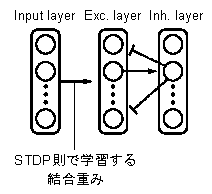
\includegraphics[scale=1.5]{figs/diehl.pdf}
    \caption{(Diehl \& Cook, 2015)で提案されたネットワーク.  1層目が入力層,2層目が興奮性ニューロン層と抑制性ニューロン層から構成されます。興奮性ニューロンと抑制性ニューロンの間の結合重みは固定で,入力層から興奮性ニューロン層へ投射される結合重みをSTDP則で学習します。}
    \label{fig:diehl}
\end{figure}
\subsection{ニューロンとシナプスのモデル}
ニューロンとシナプスのモデルとしてはConductance-basedモデルを用いています. 
\subsubsection{ニューロンのモデル}
興奮性ニューロンと抑制性ニューロンの膜電位$V$は次の式に従います. 
\begin{equation}
\tau \frac{d V}{d t}=\left(E_{\text {rest}}-V\right)+g_{e}\left(E_{\text {exc}}-V\right)+g_{i}\left(E_{\text {inh}}-V\right)    
\end{equation}
これは通常のConductance-basedモデルと同じ式ですが, ネットワークの発火率を一定に保つため, 興奮性ニューロンの膜電位の発火閾値は発火のたびに$\theta=0.05 $mV上昇するとします. 発火の無い場合は時定数$10^7$ msで減衰します. 著者実装では350 ms間, 画像をエンコードしたスパイク列を入力し, 変数をリセットするために150 ms間, 何も入力しないブランク期間を設定しています. この間に膜電位等は全てリセットされますが, 発火閾値のみ, 少し減衰するだけに留まります. さらに, 興奮性ニューロンの発火数が少ない場合には, 入力のポアソンスパイクの発火率を上げ, 再度同じ画像を提示します. 
また, 興奮性ニューロンの膜電位の時定数としては生理学的に逸脱した100 msという値を用いています. これは時定数を大きくすることで, 多くのスパイク入力を積分することができ, ノイズによる影響を減らすことができると説明されています. 
まず,準備としてこのようなニューロンを実装しておきます\footnote{コードは\texttt{./TrainingSNN/Models/Neurons.py}に含まれます. }. コード自体は2章で紹介したConductance-based LIFに修正を加えたものです。
\begin{minted}[frame=lines, framesep=2mm, baselinestretch=1.2, bgcolor=shadecolor,fontsize=\small]{python}
class DiehlAndCook2015LIF:
    def __init__(self, N, dt=1e-3, tref=5e-3, tc_m=1e-1,
                 vrest=-65, vreset=-65, init_vthr=-52, vpeak=20,
                 theta_plus=0.05, theta_max=35, tc_theta=1e4,
                 e_exc=0, e_inh=-100):
        self.N = N
        self.dt = dt
        self.tref = tref
        self.tc_m = tc_m 
        self.vreset = vreset
        self.vrest = vrest
        self.init_vthr = init_vthr
        self.theta = np.zeros(N)
        self.theta_plus = theta_plus
        self.theta_max = theta_max
        self.tc_theta = tc_theta
        self.vpeak = vpeak
        self.e_exc = e_exc \section{興奮性シナプスの平衡電位}
        self.e_inh = e_inh \section{抑制性シナプスの平衡電位}
        
        self.v = self.vreset*np.ones(N)
        self.vthr = self.init_vthr
        self.v_ = None
        self.tlast = 0
        self.tcount = 0
    
    def initialize_states(self, random_state=False):
        if random_state:
            self.v = self.vreset + \ 
                     np.random.rand(self.N)*(self.vthr-self.vreset) 
        else:
            self.v = self.vreset*np.ones(self.N)
        self.vthr = self.init_vthr
        self.theta = np.zeros(self.N)
        self.tlast = 0
        self.tcount = 0
        
    def __call__(self, g_exc, g_inh):
        I_synExc = g_exc*(self.e_exc - self.v) 
        I_synInh = g_inh*(self.e_inh - self.v)
        dv = (self.vrest - self.v + I_synExc + I_synInh) / self.tc_m
        v = self.v+((self.dt*self.tcount)>(self.tlast+self.tref))*dv*self.dt
        
        s = 1*(v>=self.vthr) #発火時は1, その他は0の出力
        
        \section{閾値の更新}
        theta = (1-self.dt/self.tc_theta)*self.theta + self.theta_plus*s
        self.theta = np.clip(theta, 0, self.theta_max)
        self.vthr = self.theta + self.init_vthr
        
        self.tlast = self.tlast*(1-s) + self.dt*self.tcount*s
        v = v*(1-s) + self.vpeak*s #閾値を超えると膜電位をvpeakにする
        self.v_ = v #発火時の電位も含めて記録するための変数
        self.v = v*(1-s) + self.vreset*s  #発火時に膜電位をリセット
        self.tcount += 1
        
        return s 
\end{minted}
追加した部分は閾値の更新のところです。最終的な閾値は\texttt{self.theta}と\texttt{self.init\_vthr}を加算した\texttt{self.vthr}を用います。変動するのは\texttt{self.theta}ですが,これはスパイクトレースと同様の実装をしています。ただし,閾値が上がりすぎることを防ぐため,上限を\texttt{self.theta\_max}として\texttt{np.clip()}により制限しています。
\subsubsection{シナプスのモデル}
シナプスにはConductance-basedの単一指数関数型シナプス(single exponential synapse)を用いています. スパイクが入るとコンダクタンス$g$は$w$だけあがり, その他では以下のように減衰します
\begin{equation}
\tau_{x} \frac{dg_x}{d t}=-g_x    
\end{equation}
ただし,$x=e, i$で,それぞれ興奮性,抑制性を意味する添え字です. なお,この実装自体は第2章で述べたものと変わりません. 
\subsection{興奮性ニューロンのラベリング}
このネットワークには出力層がなく, 通常とは異なる形式で画像を分類しています. まず, 訓練時において興奮性ニューロンの活動を全て記録します. 次に, 画像に元々されていたラベルを用いて, 興奮性の各ニューロンの各ラベルの画像への平均発火数を計算します. このとき, 各ニューロンにおいて最も発火数が多かったラベルを求め, そのラベルを各ニューロンに割り当てます. そして, 割り当てたラベルを用い, 入力画像に対する各ラベルに割り当てられたニューロンの平均発火数を求めます. このとき平均発火数が最も高いニューロン群のラベルが, 入力画像の予測ラベルとなります. また, 推論時には訓練時においてニューロンに割り当てたラベルを用います.
それではニューロンへラベルを割り当てる関数(\texttt{assign\_labels})を実装してみましょう\footnote{以降のコードは特に明記が無い限り\texttt{./TrainingSNN/LIF\_WTA\_STDP\_MNIST.py}に含まれます。また一部,BindsNETの実装を参考にしています。}。\texttt{assign\_labels}は5つの変数を引数に取ります。\texttt{spikes}は, サイズが\texttt{(n\_samples, n\_neurons)}の2次元配列で,各サンプルにおいて各興奮性ニューロンが何回発火したかを記録したものです。 \texttt{labels}はサイズが\texttt{(n\_samples, )}の配列で,各サンプルの教師ラベルを表します。\texttt{n\_labels}はラベルの数です。今回はMNISTなので10個です。 \texttt{rates}はサイズが\texttt{(n\_samples, n\_neurons)}の配列で,各興奮性ニューロンの各ラベルに対する発火率を表します。\texttt{rates}は2度目の計算以降に引数として渡すと,過去の\texttt{rates}と\texttt{alpha}によって調整される割合で指数平均を取ります。
\begin{minted}[frame=lines, framesep=2mm, baselinestretch=1.2, bgcolor=shadecolor,fontsize=\small]{python}
def assign_labels(spikes, labels, n_labels, rates=None, alpha=1.0):
    n_neurons = spikes.shape[1] 
    
    if rates is None:        
        rates = np.zeros((n_neurons, n_labels)).astype(np.float32)
    
    \section{時間の軸でスパイク数の和を取る}
    for i in range(n_labels):
        \section{サンプル内の同じラベルの数を求める}
        n_labeled = np.sum(labels == i).astype(np.int16)
    
        if n_labeled > 0:
            \section{label == iのサンプルのインデックスを取得}
            indices = np.where(labels == i)[0]
            
            \section{label == iに対する各ニューロンごとの平均発火率を計算}
            #(前回の発火率との移動平均)
            rates[:, i] = alpha*rates[:, i] + \ 
                          (np.sum(spikes[indices], axis=0)/n_labeled)
    
    sum_rate = np.sum(rates, axis=1)
    sum_rate[sum_rate==0] = 1
    \section{クラスごとの発火頻度の割合を計算する}
    proportions = rates / np.expand_dims(sum_rate, 1) \section{(n_neurons, n_labels)}
    proportions[proportions != proportions] = 0  \section{Set NaNs to 0}
    
    \section{最も発火率が高いラベルを各ニューロンに割り当てる (n_neurons,)}
    assignments = np.argmax(proportions, axis=1).astype(np.uint8) 
    return assignments, proportions, rates
\end{minted}
ここで\texttt{assignments}はサイズが\texttt{(n\_neurons,)}の配列で,各ニューロンに割り当てられたラベルを表します。これを用いて,各サンプルに対してラベルを予測する関数\texttt{prediction}を実装しましょう。
\begin{minted}[frame=lines, framesep=2mm, baselinestretch=1.2, bgcolor=shadecolor,fontsize=\small]{python}
def prediction(spikes, assignments, n_labels):    
    n_samples = spikes.shape[0]
    
    \section{各サンプルについて各ラベルの発火率を見る}
    rates = np.zeros((n_samples, n_labels)).astype(np.float32)
    
    for i in range(n_labels):
        \section{各ラベルが振り分けられたニューロンの数}
        n_assigns = np.sum(assignments == i).astype(np.uint8)
    
        if n_assigns > 0:
            \section{各ラベルのニューロンのインデックスを取得}
            indices = np.where(assignments == i)[0]
    
            \section{各ラベルのニューロンのレイヤー全体における平均発火数を求める}
            rates[:, i] = np.sum(spikes[:, indices], axis=1) / n_assigns
    
    \section{レイヤーの平均発火率が最も高いラベルを出力}
    return np.argmax(rates, axis=1).astype(np.uint8) \section{(n_samples, )}
\end{minted}
\texttt{prediction}は3つの引数, \texttt{spikes}, \texttt{assignments}, \texttt{n\_labels}を取ります。これらはそれぞれ先ほど説明した同名の配列と同じです。そして,各ラベルに紐づけられたニューロンごとに平均発火数を計算し,最も平均発火数の多かったラベルを入力サンプルのラベルとします。
\subsection{MNISTデータセットのスパイク列への変換}
入力として用いるために,MNISTデータセットをスパイク列へ変換する関数を書きましょう。MNISTデータセットを読み込む関数を別に書いても良いですが,煩雑となるため,ANNのライブラリに付属するデータ読み込み関数を利用してみます。ここでは例としてChainerの\texttt{chainer.datasets.get\_mnist()}を用いますが,他のライブラリでも大きな修正をすることなく実装できると思います。
\begin{minted}[frame=lines, framesep=2mm, baselinestretch=1.2, bgcolor=shadecolor,fontsize=\small]{python}
def online_load_and_encoding_dataset(dataset, i, dt, n_time, max_fr=32,
                                     norm=196):
    fr_tmp = max_fr*norm/np.sum(dataset[i][0])
    fr = fr_tmp*np.repeat(np.expand_dims(dataset[i][0],
                                         axis=0), n_time, axis=0)
    input_spikes = np.where(np.random.rand(n_time, 784) < fr*dt, 1, 0)
    input_spikes = input_spikes.astype(np.uint8)
    return input_spikes
\end{minted}
この関数の使用例と, スパイク列への変換が正しく行われているかを確認するコードは次のようになります。
\begin{minted}[frame=lines, framesep=2mm, baselinestretch=1.2, bgcolor=shadecolor,fontsize=\small]{python}
import chainer
dt = 1e-3; t_inj = 0.350; nt_inj = round(t_inj/dt)
train, _ = chainer.datasets.get_mnist() \section{ChainerによるMNISTデータの読み込み}
input_spikes = online_load_and_encoding_dataset(dataset=train, i=0,
                                                dt=dt, n_time=nt_inj)
\section{描画}
plt.imshow(np.reshape(np.sum(input_spikes, axis=0), (28, 28)),
           cmap="gray")
plt.show()
\end{minted}
ここでスパイク列を時間的に加算し,28$\times$28の配列に変換した後に描画をしています。結果は図\ref{fig:jitteredMNIST}のようになります。
\begin{figure}[htbp]
    \centering
    \includegraphics[scale=0.4]{figs/five.pdf}
    \caption{スパイク列に変換したMNISTデータの例(5).}
    \label{fig:jitteredMNIST}
\end{figure}
\subsection{ネットワークの実装}
それではネットワークを実装してみましょう。長いですが,それぞれの部分はこれまでの実装の組み合わせです。ただし,著者実装におけるハイパーパラメータでは正常に学習が進まなかったので,各ハイパーパラメータの値は変更しています\footnote{そもそも論文にハイパーパラメータが書いておらず,著者実装のコードを読むしかありません。}。
\begin{minted}[frame=lines, framesep=2mm, baselinestretch=1.2, bgcolor=shadecolor,fontsize=\small]{python}
class DiehlAndCook2015Network:
    def __init__(self, n_in=784, n_neurons=100, wexc=2.25, winh=0.875,
                 dt=1e-3, wmin=0.0, wmax=5e-2, lr=(1e-2, 1e-4),
                 update_nt=100):
        self.dt = dt
        self.lr_p, self.lr_m = lr
        self.wmax = wmax
        self.wmin = wmin
        self.n_neurons = n_neurons
        self.n_in = n_in
        self.norm = 0.1
        self.update_nt = update_nt
        \section{Neurons}
        self.exc_neurons = DiehlAndCook2015LIF(n_neurons, dt=dt, tref=5e-3,
                                               tc_m=1e-1,
                                               vrest=-65, vreset=-65, 
                                               init_vthr=-52,
                                               vpeak=20, theta_plus=0.05,
                                               theta_max=35,
                                               tc_theta=1e4,
                                               e_exc=0, e_inh=-100)
        self.inh_neurons = ConductanceBasedLIF(n_neurons, dt=dt, tref=2e-3,
                                               tc_m=1e-2,
                                               vrest=-60, vreset=-45,
                                               vthr=-40, vpeak=20,
                                               e_exc=0, e_inh=-85)
        \section{Synapses}
        self.input_synapse = SingleExponentialSynapse(n_in, dt=dt, td=1e-3)
        self.exc_synapse = SingleExponentialSynapse(n_neurons, dt=dt, td=1e-3)
        self.inh_synapse = SingleExponentialSynapse(n_neurons, dt=dt, td=2e-3)
        
        self.input_synaptictrace = SingleExponentialSynapse(n_in, dt=dt,
                                                            td=2e-2)
        self.exc_synaptictrace = SingleExponentialSynapse(n_neurons, dt=dt,
                                                          td=2e-2)
        
        \section{Connections (重みの初期化)}
        initW = 1e-3*np.random.rand(n_neurons, n_in)
        self.input_conn = FullConnection(n_in, n_neurons,
                                         initW=initW)
        self.exc2inh_W = wexc*np.eye(n_neurons)
        self.inh2exc_W = (winh/n_neurons)*(np.ones((n_neurons, n_neurons)) \
                          - np.eye(n_neurons))
        
        self.delay_input = DelayConnection(N=n_neurons, delay=5e-3, dt=dt)
        self.delay_exc2inh = DelayConnection(N=n_neurons, delay=2e-3, dt=dt)
        self.g_inh = np.zeros(n_neurons)
        
        self.tcount = 0
        self.s_in_ = np.zeros((self.update_nt, n_in)) 
        self.s_exc_ = np.zeros((n_neurons, self.update_nt))
        self.x_in_ = np.zeros((self.update_nt, n_in)) 
        self.x_exc_ = np.zeros((n_neurons, self.update_nt))
        
    \section{スパイクトレースのリセット}
    def reset_trace(self):
        self.s_in_ = np.zeros((self.update_nt, self.n_in)) 
        self.s_exc_ = np.zeros((self.n_neurons, self.update_nt))
        self.x_in_ = np.zeros((self.update_nt, self.n_in)) 
        self.x_exc_ = np.zeros((self.n_neurons, self.update_nt))
        self.tcount = 0
    
    \section{状態の初期化}
    def initialize_states(self):
        self.exc_neurons.initialize_states()
        self.inh_neurons.initialize_states()
        self.delay_input.initialize_states()
        self.delay_exc2inh.initialize_states()
        self.input_synapse.initialize_states()
        self.exc_synapse.initialize_states()
        self.inh_synapse.initialize_states()
        
    def __call__(self, s_in, stdp=True):
        \section{入力層}
        c_in = self.input_synapse(s_in)
        x_in = self.input_synaptictrace(s_in)
        g_in = self.input_conn(c_in)
        \section{興奮性ニューロン層}
        s_exc = self.exc_neurons(self.delay_input(g_in), self.g_inh)
        c_exc = self.exc_synapse(s_exc)
        g_exc = np.dot(self.exc2inh_W, c_exc)
        x_exc = self.exc_synaptictrace(s_exc)
        \section{抑制性ニューロン層        }
        s_inh = self.inh_neurons(self.delay_exc2inh(g_exc), 0)
        c_inh = self.inh_synapse(s_inh)
        self.g_inh = np.dot(self.inh2exc_W, c_inh)
        if stdp:
            \section{スパイク列とスパイクトレースを記録}
            self.s_in_[self.tcount] = s_in
            self.s_exc_[:, self.tcount] = s_exc
            self.x_in_[self.tcount] = x_in 
            self.x_exc_[:, self.tcount] = x_exc
            self.tcount += 1
            \section{Online STDP}
            if self.tcount == self.update_nt:
                W = np.copy(self.input_conn.W)
                
                \section{postに投射される重みが均一になるようにする}
                W_abs_sum = np.expand_dims(np.sum(np.abs(W), axis=1), 1)
                W_abs_sum[W_abs_sum == 0] = 1.0
                W *= self.norm / W_abs_sum
                
                \section{STDP則}
                dW = self.lr_p*(self.wmax-W)*np.dot(self.s_exc_, self.x_in_)
                dW -= self.lr_m*W*np.dot(self.x_exc_, self.s_in_)
                clipped_dW = np.clip(dW / self.update_nt, -5e-2, 5e-2)
                self.input_conn.W = np.clip(W + clipped_dW,
                                            self.wmin, self.wmax)
                self.reset_trace() \section{スパイク列とスパイクトレースをリセット}
        
        return s_exc
\end{minted}
ここで\texttt{\_\_call\_\_()}関数は入力スパイク列\texttt{s\_in}とSTDP則による学習をするかどうかのBoolean変数である\texttt{stdp}の2つの値を引数とします。\texttt{stdp}が\textttt{True}のとき,入力層と興奮性ニューロン層のスパイク列,スパイクトレースが記録され,\texttt{self.tcount}が\textttt{self.update\_nt}となったときにSTDP則による重みの更新が行われます。重みの更新の前に,興奮性ニューロンへ投射される重みの合計が\texttt{self.norm}となるように正規化をしています。また,ここでのSTDP則は重み依存的なものとしています。なお,重みの更新時に重みが
\texttt{self.wmin}と\texttt{self.wmax}範囲となるように\texttt{np.clip()}で制限をしています。
\subsection{学習イテレーションと結果の表示}
実際にシミュレーションをする部分を書いていきます。タイムステップは1 msとし,350 msの間は画像を変換したスパイク列を入力,150 msの間何も入力しない,というようにします。また,興奮性ニューロンの数は100個とし,訓練データのサンプル数は10000, エポック数は20とします。
なお,学習後にネットワークの評価をするために,このファイル内の関数を呼び出します。そのため,この部分は外部から呼び出されないように\texttt{if \_\_name\_\_ == '\_\_main\_\_':}と記述した中に書いておきます。
\begin{minted}[frame=lines, framesep=2mm, baselinestretch=1.2, bgcolor=shadecolor,fontsize=\small]{python}
if __name__ == '__main__':
    \section{350ms画像入力,150ms入力なしでリセットさせる(膜電位の閾値以外)}
    dt = 1e-3 \section{タイムステップ(sec)}
    t_inj = 0.350 \section{刺激入力時間(sec)}
    t_blank = 0.150 \section{ブランク時間(sec)}
    nt_inj = round(t_inj/dt)
    nt_blank = round(t_blank/dt)
    
    n_neurons = 100 \section{興奮性/抑制性ニューロンの数}
    n_labels = 10 \section{ラベル数}
    n_epoch = 20 \section{エポック数}
    
    n_train = 10000 \section{訓練データの数}
    update_nt = nt_inj \section{STDP則による重みの更新間隔}
    
    \section{ChainerによるMNISTデータの読み込み}
    train, _ = chainer.datasets.get_mnist()
    labels = np.array([train[i][1] for i in range(n_train)]) \section{ラベルの配列}
    
    \section{ネットワークの定義}
    network = DiehlAndCook2015Network(n_in=784, n_neurons=n_neurons,
                                      wexc=2.25, winh=0.875,
                                      dt=dt, wmin=0.0, wmax=0.1,
                                      lr=(1e-2, 1e-4),
                                      update_nt=update_nt)
    
    network.initialize_states() \section{ネットワークの初期化}
    spikes = np.zeros((n_train, n_neurons)).astype(np.uint8) \section{スパイク記録変数}
    accuracy_all = np.zeros(n_epoch) \section{訓練精度を記録する変数}
    blank_input = np.zeros(784) \section{ブランク入力}
    init_max_fr = 32 \section{初期のポアソンスパイクの最大発火率}
    
    \section{結果を保存するディレクトリ}
    results_save_dir = "./LIF_WTA_STDP_MNIST_results/"
    os.makedirs(results_save_dir, exist_ok=True) \section{ディレクトリが無ければ作成}
    
    \section{Simulation}
    for epoch in range(n_epoch):
        for i in tqdm(range(n_train)):
            max_fr = init_max_fr
            while(True):
                \section{入力スパイクをオンラインで生成}
                input_spikes = online_load_and_encoding_dataset(train, i, dt,
                                                                nt_inj,
                                                                max_fr)
                spike_list = [] \section{サンプルごとにスパイクを記録するリスト}
                \section{画像刺激の入力}
                for t in range(nt_inj):
                    s_exc = network(input_spikes[t], stdp=True)
                    spike_list.append(s_exc)
                
                \section{スパイク数を記録}
                spikes[i] = np.sum(np.array(spike_list), axis=0)
                
                \section{ブランク刺激の入力}
                for _ in range(nt_blank):
                    _ = network(blank_input, stdp=False)
    
                \section{スパイク数を計算}
                num_spikes_exc = np.sum(np.array(spike_list))
                \section{スパイク数が5より大きければ次のサンプルへ}
                if num_spikes_exc >= 5:
                    break
                else: \section{スパイク数が5より小さければ入力発火率を上げて再度刺激}
                    max_fr += 16
        
        \section{ニューロンを各ラベルに割り当てる}
        if epoch == 0:
            assignments, proportions, rates = assign_labels(spikes, labels,
                                                            n_labels)
        else:
            assignments, proportions, rates = assign_labels(spikes, labels,
                                                            n_labels, rates)
        print("Assignments:\n", assignments)
        
        \section{スパイク数の確認(正常に発火しているか確認)}
        sum_nspikes = np.sum(spikes, axis=1)
        mean_nspikes = np.mean(sum_nspikes).astype(np.float16)
        print("Ave. spikes:", mean_nspikes)
        print("Min. spikes:", sum_nspikes.min())
        print("Max. spikes:", sum_nspikes.max())
    
        \section{入力サンプルのラベルを予測する}
        predicted_labels = prediction(spikes, assignments, n_labels)
        
        \section{訓練精度を計算}
        accuracy = np.mean(np.where(labels==predicted_labels, 1, 0))
        print("epoch :", epoch, " accuracy :", accuracy)
        accuracy_all[epoch] = accuracy
        
        \section{学習率の減衰}
        network.lr_p *= 0.85
        network.lr_m *= 0.85
        
        \section{重みの保存(エポック毎)}
        np.save(results_save_dir+"weight_epoch"+str(epoch)+".npy",
                network.input_conn.W)
        
    \section{結果}
    plt.figure(figsize=(5,4))
    plt.plot(np.arange(1, n_epoch+1), accuracy_all*100,
             color="k")
    plt.xlabel("Epoch")
    plt.ylabel("Train accuracy (%)")
    plt.savefig(results_save_dir+"accuracy.png")
    
    np.save(results_save_dir+"assignments.npy", assignments)
    np.save(results_save_dir+"weight.npy", network.input_conn.W)
    np.save(results_save_dir+"exc_neurons_theta.npy",
            network.exc_neurons.theta)
\end{minted}
シミュレーション部は入れ子状のループとなっています。\texttt{while}によるループは, サンプルを入力した時に興奮性ニューロン全体の発火数が5を超えない限り, 入力の発火率を増加させて再度スパイク列を入力する,ということを行います。
各エポック終了時には刺激時の興奮性ニューロンの発火情報から,興奮性ニューロンの各ラベルへの割り当てと各サンプルのラベルの予測,および訓練精度の計算を行います。最後にSTDP則における学習率を減衰させます。
学習が終了した後は訓練精度の変化と各ニューロンに割り当てたラベル(\texttt{assignments}),入力層から興奮性ニューロンへの結合重み,興奮性ニューロンの閾値を保存しておきます。なお,学習時における訓練精度の変化は図\ref{fig:MNISTaccuracy}のようになりました。
\begin{figure}[htbp]
    \centering
    \includegraphics[scale=0.5]{figs/accuracy.pdf}
    \caption{訓練時の精度の変化. 最終的な訓練精度は69.9\%となりました。}
    \label{fig:MNISTaccuracy}
\end{figure}
\subsection{ネットワークの評価}
学習後のネットワークを学習に用いなかったテストデータで評価してみましょう。
\footnote{コードは\texttt{./TrainingSNN/LIF\_WTA\_STDP\_MNIST\_evaluation.py}です。}。ほぼネットワークの学習の際に記述したコードを流用するだけです。まず,学習後の重みを読み込んで,テストデータ(1000サンプル)を入力し,それに対するスパイクを記録します。次に訓練時に行った各ニューロンのラベルへの割り当てを用いて各サンプルのラベルを予測し,実際のラベルと比較し,推論精度を計算します。
\begin{minted}[frame=lines, framesep=2mm, baselinestretch=1.2, bgcolor=shadecolor,fontsize=\small]{python}
import chainer
from LIF_WTA_STDP_MNIST import online_load_and_encoding_dataset, prediction
from LIF_WTA_STDP_MNIST import DiehlAndCook2015Network
\section{350ms画像入力,150ms入力なしでリセットさせる(膜電位の閾値以外)}
dt = 1e-3 \section{タイムステップ(sec)}
t_inj = 0.350 \section{刺激入力時間(sec)}
t_blank = 0.150 \section{ブランク時間(sec)}
nt_inj = round(t_inj/dt)
nt_blank = round(t_blank/dt)
n_neurons = 100 #興奮性/抑制性ニューロンの数
n_labels = 10 #ラベル数
n_train = 1000 \section{訓練データの数}
update_nt = nt_inj \section{STDP則による重みの更新間隔}
_, test = chainer.datasets.get_mnist() \section{ChainerによるMNISTデータの読み込み}
labels = np.array([test[i][1] for i in range(n_train)]) \section{ラベルの配列}
\section{結果が保存されているディレクトリ}
results_save_dir = "./LIF_WTA_STDP_MNIST_results/"
\section{ネットワークの定義}
network = DiehlAndCook2015Network(n_in=784, n_neurons=n_neurons,
                                  wexc=2.25, winh=0.875,
                                  dt=dt, wmin=0.0, wmax=0.1,
                                  lr=(1e-2, 1e-4),
                                  update_nt=update_nt)
network.initialize_states() \section{ネットワークの初期化}
\section{重みと閾値のload}
network.input_conn.W = np.load(results_save_dir+"weight.npy")
network.exc_neurons.theta = np.load(results_save_dir+"exc_neurons_theta.npy")
network.exc_neurons.theta_plus = 0 \section{閾値が上昇しないようにする}
#スパイクを記録する変数
spikes = np.zeros((n_train, n_neurons)).astype(np.uint8)
blank_input = np.zeros(784) \section{ブランク入力}
init_max_fr = 32 \section{初期のポアソンスパイクの最大発火率}
for i in tqdm(range(n_train)):
    max_fr = init_max_fr
    while(True):
        \section{入力スパイクをオンラインで生成}
        input_spikes = online_load_and_encoding_dataset(test, i, dt,
                                                        nt_inj, max_fr)
        spike_list = [] \section{サンプルごとにスパイクを記録するリスト}
        \section{画像刺激の入力}
        for t in range(nt_inj):
            s_exc = network(input_spikes[t], stdp=False)
            spike_list.append(s_exc)
        
        spikes[i] = np.sum(np.array(spike_list), axis=0) \section{スパイク数を記録}
        
        \section{ブランク刺激の入力}
        for _ in range(nt_blank):
            _ = network(blank_input, stdp=False)
        num_spikes_exc = np.sum(np.array(spike_list)) \section{スパイク数を計算}
        if num_spikes_exc >= 5: \section{スパイク数が5より大きければ次のサンプルへ}
            break
        else: \section{スパイク数が5より小さければ入力発火率を上げて再度刺激}
            max_fr += 16
            
\section{入力サンプルのラベルを予測する}
assignments = np.load(results_save_dir+"assignments.npy")
predicted_labels = prediction(spikes, assignments, n_labels)
\section{訓練精度を計算}
accuracy = np.mean(np.where(labels==predicted_labels, 1, 0))
print("Test accuracy :", accuracy)
\end{minted}
実行した結果,\colorbox{shadecolor}{\texttt{Test accuracy : 0.653}}となり,テストデータ(1000サンプル)での精度は65.3\%となりました。100個のニューロンを学習させた際の論文における精度が約85\%であるので,それに比べるとかなり低い値です。これには学習データを少なくしている,ハイパーパラメータを著者実装とは異なるものにしているということなどが原因であると考えられます。
\subsection{興奮性ニューロンの受容野の描画}
最後に,学習後の入力層から興奮性ニューロン層へのシナプス重みを描画してみましょう\footnote{コードは\texttt{./TrainingSNN/LIF\_WTA\_STDP\_MNIST\_visualize\_weights.py}です。}。各興奮性ニューロンへ投射する784個のシナプス重みを28$\times$28に\texttt{reshape}して描画するだけです。
\begin{minted}[frame=lines, framesep=2mm, baselinestretch=1.2, bgcolor=shadecolor,fontsize=\small]{python}
epoch = 19
n_neurons = 100
\section{結果が保存されているディレクトリ}
results_save_dir = "./LIF_WTA_STDP_MNIST_results/"
input_conn_W = np.load(results_save_dir+"weight_epoch"+str(epoch)+".npy")
reshaped_W = np.reshape(input_conn_W, (n_neurons, 28, 28))
\section{描画}
fig = plt.figure(figsize=(6,6))
fig.subplots_adjust(left=0, right=1, bottom=0, top=1,
                    hspace=0.05, wspace=0.05)
row = col = np.sqrt(n_neurons)
for i in tqdm(range(n_neurons)):
  ax = fig.add_subplot(row, col, i+1, xticks=[], yticks=[])
  ax.imshow(reshaped_W[i], cmap="gray")
plt.savefig("weights_"+str(epoch)+".png")
plt.show()
\end{minted}
結果は図\ref{fig:Diehl_weights}のようになります。
\begin{figure}[htbp]
 \begin{minipage}{0.5\hsize}
  \begin{center}
   \includegraphics[width=60mm]{figs/weights_0.pdf}
  \end{center}
 \end{minipage}
 \begin{minipage}{0.5\hsize}
  \begin{center}
   \includegraphics[width=60mm]{figs/weights_19.pdf}
  \end{center}
 \end{minipage}
\caption{学習後の100個の興奮性ニューロンの重みを描画したもの。各数字に対応するフィルターが生まれていることが分かります。(左) 1エポック終了時の重み。受容野が生じつつあるのが分かります。(右) 20エポック終了時。一番上の段の10個のニューロンをラベルに割り当てた結果は``5, 2, 6, 3, 3, 9, 4, 3, 0, 2"となっており,受容野の見た目と一致しています。}
\label{fig:Diehl_weights}
\end{figure}
\end{document}

% \section{ロジスティック回帰とパーセプトロン}
logistic regression, perceptron
1層パーセプトロン
\url{https://www.cs.utexas.edu/~gdurrett/courses/fa2022/perc-lr-connections.pdf}
add SyntheticDatasets
よりも正規分布×2の方がいいか
\url{https://en.wikipedia.org/wiki/Perceptron}

\url{https://arxiv.org/abs/2012.03642}


perceptronは0/1 or -1/1のどちらか

UNDERSTANDING STRAIGHT-THROUGH ESTIMATOR IN TRAINING ACTIVATION QUANTIZED NEURAL NETS

Yoshua Bengio, Nicholas L´eonard, and Aaron Courville. Estimating or propagating gradients through stochastic neurons for conditional computation. arXiv preprint arXiv:1308.3432, 2013.

Hinton (2012) in his lecture 15b

G. Hinton. Neural networks for machine learning, 2012.
\url{https://www.cs.toronto.edu/~hinton/coursera_lectures.html}

delta rule
\lstinputlisting[language=julia]{./text/local-learning-rule/logistic-regression-perceptron/003.jl}
\lstinputlisting[language=julia]{./text/local-learning-rule/logistic-regression-perceptron/004.jl}
\lstinputlisting[language=julia]{./text/local-learning-rule/logistic-regression-perceptron/005.jl}
\lstinputlisting[language=julia]{./text/local-learning-rule/logistic-regression-perceptron/006.jl}
\begin{figure}[ht]
	\centering
	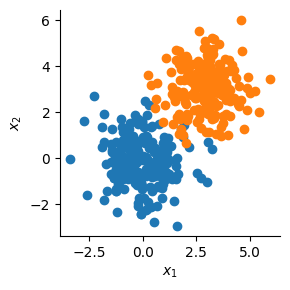
\includegraphics[scale=0.8, max width=\linewidth]{./fig/local-learning-rule/logistic-regression-perceptron/cell006.png}
	\caption{cell006.png}
	\label{cell006.png}
\end{figure}
\lstinputlisting[language=julia]{./text/local-learning-rule/logistic-regression-perceptron/007.jl}
\lstinputlisting[language=julia]{./text/local-learning-rule/logistic-regression-perceptron/008.jl}
\lstinputlisting[language=julia]{./text/local-learning-rule/logistic-regression-perceptron/009.jl}
\begin{figure}[ht]
	\centering
	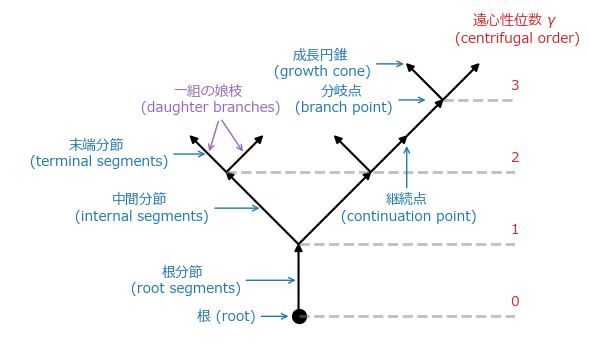
\includegraphics[scale=0.8, max width=\linewidth]{./fig/neuron-model/neurite-growth-model/cell009.png}
	\caption{cell009.png}
	\label{cell009.png}
\end{figure}
Here σ denotes the (point-wise) activation function, $W \in R^{m\times n}$
is the weight-matrix and $b \in R^n$
is
the bias-vector. The vector $x \in R^m$ and the vector $y \in R^n$ denote the input, respectively the output


\begin{equation}
y=\sigma(W^\top x + b)
\end{equation}



\begin{align}
& \text { Initialize } W^0, b^0 \text {; } \\
& \text { for } k=1,2, \ldots \text { do } \\
& \qquad \begin{array}{|l}
\text { for } i=1, \ldots, s \text { do } \\
e_i=y_i-\sigma\left(\left(W^k\right)^{\top} x_i+b^k\right) \\
W^{k+1}=W^k+e_i x_i^{\top} \\
b^{k+1}=b^k+e_i
\end{array} \\
& \text { end }
\end{align}
\lstinputlisting[language=julia]{./text/local-learning-rule/logistic-regression-perceptron/011.jl}
\lstinputlisting[language=julia]{./text/local-learning-rule/logistic-regression-perceptron/012.jl}
\begin{figure}[ht]
	\centering
	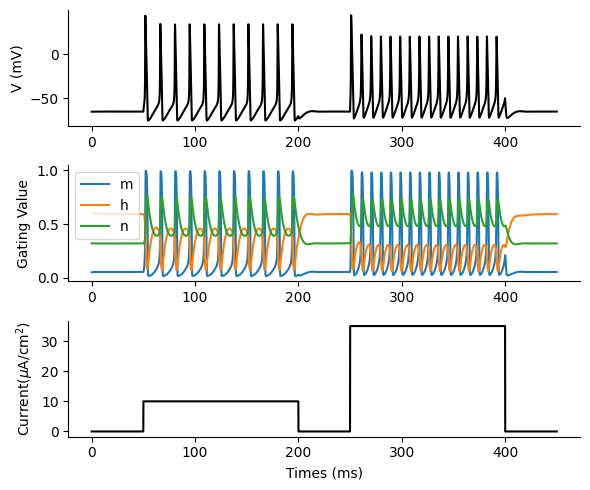
\includegraphics[scale=0.8, max width=\linewidth]{./fig/neuron-model/hodgkin-huxley/cell012.png}
	\caption{cell012.png}
	\label{cell012.png}
\end{figure}
\lstinputlisting[language=julia]{./text/local-learning-rule/logistic-regression-perceptron/013.jl}
\lstinputlisting[language=julia]{./text/local-learning-rule/logistic-regression-perceptron/014.jl}
ax + by + c = 0  
y = -a/b x - c/b
\lstinputlisting[language=julia]{./text/local-learning-rule/logistic-regression-perceptron/016.jl}
\lstinputlisting[language=julia]{./text/local-learning-rule/logistic-regression-perceptron/017.jl}
\begin{figure}[ht]
	\centering
	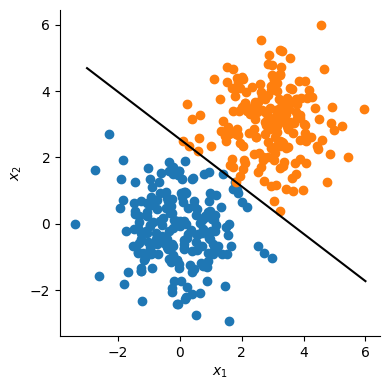
\includegraphics[scale=0.8, max width=\linewidth]{./fig/local-learning-rule/logistic-regression-perceptron/cell017.png}
	\caption{cell017.png}
	\label{cell017.png}
\end{figure}
 % ok2
% \section{自己組織化マップと視覚野の構造}
視覚野にはコラム構造が存在する.こうした構造は神経活動依存的な発生  (activity dependent development) により獲得される.本節では視覚野のコラム構造を生み出す数理モデルの中で,\textbf{自己組織化マップ (self-organizing map)}\index{じこそしきかまっぷ (self-organizing map)@自己組織化マップ (self-organizing map)} \citep{Kohonen1982-mn}, \citep{Kohonen2013-yt}を取り上げる.

自己組織化マップを視覚野の構造に適応したのは\citep{Obermayer1990-gq} \citep{N_V_Swindale1998-ri}などの研究である.視覚野マップの数理モデルとして自己組織化マップは受容野を考慮しないなどの簡略化がなされているが,単純な手法にして視覚野の構造に関する良い予測を与える.他の数理モデルとしては自己組織化マップと発想が類似している \textbf{Elastic net}\index{Elastic net}  \citep{Durbin1987-bp} \citep{Durbin1990-xx} \citep{Carreira-Perpinan2005-gy} (ここでのElastic netは正則化手法としてのElastic net regularizationとは異なる)や受容野を明示的に設定した \citep{Tanaka2004-vz}, \citep{Ringach2007-oe}などのモデルがある.総説としては\citep{Das2005-mq},\citep{Goodhill2007-va} ,数理モデル同士の関係については\citep{2002-nm}が詳しい.

自己組織化マップでは「抹消から中枢への伝達過程で損失される情報量」,および「近い性質を持ったニューロン同士が結合するような配線長」の両者を最小化するような学習が行われる.包括性 (coverage) と連続性 (continuity) のトレードオフとも呼ばれる \citep{Carreira-Perpinan2005-gy}  (Elastic netは両者を明示的に計算し,線形結合で表されるエネルギー関数を最小化する.Elastic netは本書では取り扱わないが,MATLAB実装が公開されている
\url{https://faculty.ucmerced.edu/mcarreira-perpinan/research/EN.html}) . 連続性と関連する事項として,近い性質を持つ細胞が脳内で近傍に存在する現象があり,これを\textbf{トポグラフィックマッピング (topographic mapping)}\index{とぽぐらふぃっくまっぴんぐ (topographic mapping)@トポグラフィックマッピング (topographic mapping)} と呼ぶ.トポグラフィックマッピングの数理モデルの初期の研究としては\citep{Von_der_Malsburg1973-bz} \citep{Willshaw1976-zo} \citep{Takeuchi1979-mi}などがある.

発生の数理モデルに関する総説 \citep{Van_Ooyen2011-fz}, \citep{Goodhill2018-ho}
\subsection{単純なデータセット}
SOMにおける$n$番目の入力を $\mathbf{v}(t)=\mathbf{v}_n\in \mathbb{R}^{D} (n=1, \ldots, N)$,$m$番目のニューロン$ (m=1, \ldots, M) $の重みベクトル (または活動ベクトル, 参照ベクトル) を$\mathbf{w}_m(t)\in \mathbb{R}^{D}$とする \citep{Kohonen2013-yt}.また,各ニューロンの物理的な位置を$\mathbf{x}_m$とする.このとき,$\mathbf{v}(t)$に対して$\mathbf{w}_m(t)$を次のように更新する.

まず,$\mathbf{v}(t)$と$\mathbf{w}_m(t)$の間の距離が最も小さい (類似度が最も大きい) ニューロンを見つける.距離や類似度としてはユークリッド距離やコサイン類似度などが考えられる.


\begin{align}
&[\text{ユークリッド距離}]: c = \underset{m}{\operatorname{argmin}}\left[\|\mathbf{v}(t)-\mathbf{w}_m(t)\|^2\right]\\
&[\text{コサイン類似度}]: c  = \underset{m}{\operatorname{argmax}}\left[\frac{\mathbf{w}_m(t)^\top\mathbf{v}(t)}{\|\mathbf{w}_m(t)\|\|\mathbf{v}(t)\|}\right]
\end{align}


この,$c$番目のニューロンを\textbf{勝者ユニット(best matching unit; BMU)}\index{しょうしゃゆにっと(best matching unit; BMU)@勝者ユニット(best matching unit; BMU)} と呼ぶ.コサイン類似度において,$\mathbf{w}_m(t)^\top\mathbf{v}(t)$は線形ニューロンモデルの出力となる.このため,コサイン距離を採用する方が生理学的に妥当でありSOMの初期の研究ではコサイン類似度が用いられている \citep{Kohonen1982-mn}.しかし,コサイン類似度を用いる場合は$\mathbf{w}_m$および$\mathbf{v}$を正規化する必要がある.ユークリッド距離を用いると正規化なしでも学習できるため,SOMを応用する上ではユークリッド距離が採用される事が多い.ユークリッド距離を用いる場合,$\mathbf{w}_m$は重みベクトルではなくなるため,活動ベクトルや参照ベクトルと呼ばれる.ここでは結果の安定性を優先してユークリッド距離を用いることとする.

こうして得られた$c$を用いて$\mathbf{w}_m$を次のように更新する.


\begin{equation}
\mathbf{w}_m(t+1)=\mathbf{w}_m(t)+h_{cm}(t)[\mathbf{v}(t)-\mathbf{w}_m(t)]
\end{equation}


ここで$h_{cm}(t)$は近傍関数 (neighborhood function) と呼ばれ,$c$番目と$m$番目のニューロンの距離が近いほど大きな値を取る.ガウス関数を用いるのが一般的である.


\begin{equation}
h_{cm}(t)=\alpha(t)\exp\left(-\frac{\|\mathbf{x}_c-\mathbf{x}_m\|^2}{2\sigma^2(t)}\right)
\end{equation}


ここで$\mathbf{x}$はニューロンの位置を表すベクトルである.また,$\alpha(t), \sigma(t)$は単調に減少するように設定する.\footnote{Generative topographic map (GTM)を用いれば$\alpha(t), \sigma(t)$の縮小は必要ない.また,SOMとGTMの間を取ったモデルとしてS-mapがある.}
\lstinputlisting[language=julia]{./text/local-learning-rule/self-organizing-map/002.jl}
ToDo: dimsをv, wで修正
\lstinputlisting[language=julia]{./text/local-learning-rule/self-organizing-map/004.jl}
\lstinputlisting[language=julia]{./text/local-learning-rule/self-organizing-map/005.jl}
\lstinputlisting[language=julia]{./text/local-learning-rule/self-organizing-map/006.jl}
\lstinputlisting[language=julia]{./text/local-learning-rule/self-organizing-map/007.jl}
近傍関数 (neighborhood function)のための二次元ガウス関数を実装する.Winnerニューロンからの距離に応じて値が減弱する関数である.ここでは一つの入力に対して全てのニューロンの活動ベクトルを更新するということはせず,winner neuronの近傍のニューロンのみ更新を行う.つまり,更新においてはglobalではなくlocalな処理のみを行うということである  (Winner neuronの決定にはWTAによるglobalな評価が必要ではあるが) .
自己組織化マップのメインとなる関数を書く.ナイーブに実装する.この方法だと空間が円,球体やトーラスのように周期性を持つ場合にも適応できる.
\lstinputlisting[language=julia]{./text/local-learning-rule/self-organizing-map/010.jl}
今回のように2次元のみを扱う場合はwinner neuronの周辺だけをsliceで抜き出して重み更新する方が高速である.
\lstinputlisting[language=julia]{./text/local-learning-rule/self-organizing-map/012.jl}
\lstinputlisting[language=julia]{./text/local-learning-rule/self-organizing-map/013.jl}
\lstinputlisting[language=julia]{./text/local-learning-rule/self-organizing-map/014.jl}
青点が$\mathbf{v}$,オレンジの点が$\mathbf{w}$である.黒線はニューロン間の位置関係を表す (これはWeight unfolding diagramsと呼ばれる).下段のヒートマップは$\mathbf{w}$の一番目の次元を表す.学習が進むとともに近傍のニューロンが近い活動ベクトルを持つことがわかる.
\lstinputlisting[language=julia]{./text/local-learning-rule/self-organizing-map/016.jl}
\lstinputlisting[language=julia]{./text/local-learning-rule/self-organizing-map/017.jl}
\begin{figure}[ht]
	\centering
	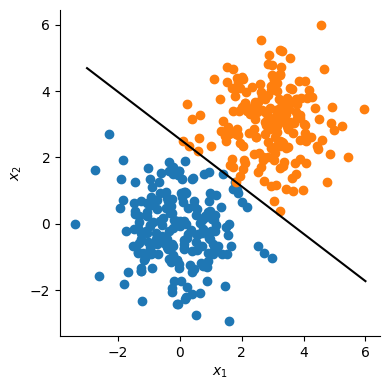
\includegraphics[scale=0.8, max width=\linewidth]{./fig/local-learning-rule/logistic-regression-perceptron/cell017.png}
	\caption{cell017.png}
	\label{cell017.png}
\end{figure}
unified distance matrixを描画する.隣接する要素とは位置の差の絶対値が1であることを利用する.
\lstinputlisting[language=julia]{./text/local-learning-rule/self-organizing-map/019.jl}
\lstinputlisting[language=julia]{./text/local-learning-rule/self-organizing-map/020.jl}
\lstinputlisting[language=julia]{./text/local-learning-rule/self-organizing-map/021.jl}
\lstinputlisting[language=julia]{./text/local-learning-rule/self-organizing-map/022.jl}
複数の点が同じ位置に重なっていることに注意.
\lstinputlisting[language=julia]{./text/local-learning-rule/self-organizing-map/024.jl}
\begin{figure}[ht]
	\centering
	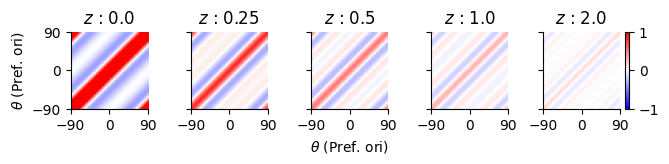
\includegraphics[scale=0.8, max width=\linewidth]{./fig/bayesian-brain/neural-sampling/cell024.png}
	\caption{cell024.png}
	\label{cell024.png}
\end{figure}
\subsection{視覚野マップ}
集合の直積を配列として返す関数 \jl{product}と極座標を直交座標に変換する関数 \jl{pol2cart}を用意する.
\lstinputlisting[language=julia]{./text/local-learning-rule/self-organizing-map/026.jl}
刺激と初期の活動ベクトルは\citep{Carreira-Perpinan2005-gy} を参考に作成.直積\jl{product}で全ての組の入力を作成する.
\lstinputlisting[language=julia]{./text/local-learning-rule/self-organizing-map/028.jl}
\lstinputlisting[language=julia]{./text/local-learning-rule/self-organizing-map/029.jl}
\lstinputlisting[language=julia]{./text/local-learning-rule/self-organizing-map/030.jl}
描画用関数を実装する. \jl{w_history}を用いてアニメーションを作成すると発達の過程が可視化されるが,これは読者への課題とする.
\lstinputlisting[language=julia]{./text/local-learning-rule/self-organizing-map/032.jl}
\lstinputlisting[language=julia]{./text/local-learning-rule/self-organizing-map/033.jl}
\begin{figure}[ht]
	\centering
	\includegraphics[scale=0.8, max width=\linewidth]{./fig/local-learning-rule/self-organizing-map/cell033.png}
	\caption{cell033.png}
	\label{cell033.png}
\end{figure}
 % ok2

\chapter{生成モデルとエネルギーベースモデル}
% \section{エネルギーベースモデル}
本章では\textbf{\index{えねるぎーべーすもでる (energy-based models; EBMs)@エネルギーベースモデル (energy-based models; EBMs)}} という枠組みに含まれるモデルを紹介する.エネルギーベースモデルではネットワークの状態をスカラー値に変換するエネルギー関数 (あるいはコスト関数) を定義し,推論時と学習時の双方においてエネルギーを最小化するようにネットワークの状態を更新する.\cite{LeCun2006-dt}

入力 $\mathbf{x}\in \mathbb{R}^d$, エネルギー関数 $E_\theta: \mathbb{R}^d\to \mathbb{R}$を考える.


\begin{align}
p_\theta(\mathbf{x})&=\frac{\exp(-E_\theta(\mathbf{x}))}{Z_\theta}\\
Z_\theta &= \int \exp(-E_\theta(\mathbf{x})) d\mathbf{x}
\end{align}


$Z_\theta$は分配関数.
 % ok
% \section{Hopfield モデル}


\cite{Hopfield1982-vu}で提案.始めは1と0の状態を取った.

Hopfieldモデルと呼ばれることが多いが,Amariの先駆的研究\cite{Amari1972-fq}を踏まえAmari-Hopfieldモデルと呼ばれることもある.

次のような連続時間線形モデルを考える.シナプス前活動を$\mathbf{x}\in \mathbb{R}^n$, 後活動を$\mathbf{y}\in \mathbb{R}^m$, 重み行列を$\mathbf{W}\in \mathbb{R}^{m\times n}$とする.


\begin{equation}
\frac{d\mathbf{y}}{dt}=-\mathbf{y}+\mathbf{W}\mathbf{x}+\mathbf{b}
\end{equation}


ここで$\dfrac{\partial\mathcal{L}}{\partial\mathbf{y}}:=-\dfrac{d\mathbf{y}}{dt}$となるような$\mathcal{L}\in \mathbb{R}$を仮定すると,


\begin{equation}
\mathcal{L}=\int \left(\mathbf{y}-\mathbf{W}\mathbf{x}-\mathbf{b}\right)\ d\mathbf{y}=\frac{1}{2}\|\mathbf{y}\|^2-\mathbf{y}^\top \mathbf{W}\mathbf{x}-\mathbf{y}^\top \mathbf{b}
\end{equation}


となる. これをさらに$\mathbf{W}$で微分すると,


\begin{equation}
\dfrac{\partial\mathcal{L}}{\partial\mathbf{W}}=-\mathbf{y}\mathbf{x}^\top\Rightarrow
\frac{d\mathbf{W}}{dt}=-\dfrac{\partial\mathcal{L}}{\partial\mathbf{W}}=\mathbf{y}\mathbf{x}^\top=(\text{post})\cdot (\text{pre})^\top
\end{equation}


となり,Hebb則が導出できる.
\subsection{モデルの定義}
モデルを定義する.
\lstinputlisting[language=julia]{./text/energy-based-model/hopfield-model/002.jl}
\lstinputlisting[language=julia]{./text/energy-based-model/hopfield-model/003.jl}
\lstinputlisting[language=julia]{./text/energy-based-model/hopfield-model/004.jl}
データセットの作成
\lstinputlisting[language=julia]{./text/energy-based-model/hopfield-model/006.jl}
\lstinputlisting[language=julia]{./text/energy-based-model/hopfield-model/007.jl}
\begin{figure}[ht]
	\centering
	\includegraphics[scale=0.8, max width=\linewidth]{./fig/bayesian-brain/neural-sampling/cell007.png}
	\caption{cell007.png}
	\label{cell007.png}
\end{figure}
モデルの定義と訓練
\lstinputlisting[language=julia]{./text/energy-based-model/hopfield-model/009.jl}
\lstinputlisting[language=julia]{./text/energy-based-model/hopfield-model/010.jl}
\begin{figure}[ht]
	\centering
	\includegraphics[scale=0.8, max width=\linewidth]{./fig/introduction/linear-regression/cell010.png}
	\caption{cell010.png}
	\label{cell010.png}
\end{figure}
画像の復元を行う.
エネルギー関数


\begin{equation}
E=-{\frac 12}\sum _{{i,j}}{w_{{ij}}{s_{i}}{s_{j}}}+\sum _{i}{\theta _{i}}{s_{i}}=-{\frac 12}\mathbf{s}^\top\mathbf{W}\mathbf{s}+\mathbf{\theta}^\top\mathbf{s}
\end{equation}


を最小化するように内部状態 $\mathbf{s}$ を更新.


\begin{equation}
\mathbf{s}\leftarrow \text{sign}\left(\mathbf{W}\mathbf{s}-\mathbf{\theta}\right)
\end{equation}
\lstinputlisting[language=julia]{./text/energy-based-model/hopfield-model/012.jl}
\lstinputlisting[language=julia]{./text/energy-based-model/hopfield-model/013.jl}
\lstinputlisting[language=julia]{./text/energy-based-model/hopfield-model/014.jl}
\begin{figure}[ht]
	\centering
	\includegraphics[scale=0.8, max width=\linewidth]{./fig/energy-based-model/hopfield-model/cell014.png}
	\caption{cell014.png}
	\label{cell014.png}
\end{figure}
\subsection{稠密連想記憶 (dense associative memory) モデル}
\textbf{Dense Associative Memory (DAM)} モデル (Modern Hopfield networksとも呼ばれる) .

\begin{itemize}
\item Krotov, Dmitry, and John J. Hopfield. 2016. “Dense Associative Memory for Pattern Recognition.” arXiv. arXiv. \url{http://arxiv.org/abs/1606.01164}.
\item Krotov, Dmitry, and John Hopfield. 2018. “Dense Associative Memory Is Robust to Adversarial Inputs.” Neural Computation 30 (12): 3151–67.
\item Krotov, Dmitry, and John J. Hopfield. 2019. “Unsupervised Learning by Competing Hidden Units.” Proceedings of the National Academy of Sciences of the United States of America 116 (16): 7723–31.
\end{itemize}


\begin{itemize}
\item Ramsauer, Hubert, Bernhard Schäfl, Johannes Lehner, Philipp Seidl, Michael Widrich, Thomas Adler, Lukas Gruber, et al. 2020. “Hopfield Networks Is All You Need.” arXiv. arXiv. \url{http://arxiv.org/abs/2008.02217}.
\end{itemize}

深層ニューラルネットワークへの応用.


\begin{itemize}
\item Krotov, Dmitry, and John J. Hopfield. 2020. “Large Associative Memory Problem in Neurobiology and Machine Learning.” \url{https://openreview.net/pdf?id=X4y_10OX-hX}
\end{itemize}

“Hopfield Networks Is All You Need.”の論文における非生理学的3ニューロン相互作用の緩和.
 % ok
% \section{Boltzmann マシン}
\subsection{Boltzmann マシン}
(Boltzmann machine)
\subsection{制限 Boltzmann マシン}
(Restricted Boltzmann machine) 
(cf.) \url{http://deeplearning.net/tutorial/rbm.html}
データの読み込み
\lstinputlisting[language=julia]{./text/energy-based-model/boltzmann-machine/003.jl}
\lstinputlisting[language=julia]{./text/energy-based-model/boltzmann-machine/004.jl}
\lstinputlisting[language=julia]{./text/energy-based-model/boltzmann-machine/005.jl}
\begin{figure}[ht]
	\centering
	\includegraphics[scale=0.8, max width=\linewidth]{./fig/solve-credit-assignment-problem/linear-network-learning-dynamics/cell005.png}
	\caption{cell005.png}
	\label{cell005.png}
\end{figure}
\lstinputlisting[language=julia]{./text/energy-based-model/boltzmann-machine/006.jl}
\lstinputlisting[language=julia]{./text/energy-based-model/boltzmann-machine/007.jl}
離散の観測変数(visible variable) $\mathbf{v}$, 潜在変数(hidden variable) $\mathbf{h}$とする.各ユニットの値は$\{0, 1\}$の2値 (binary)である.

エネルギー関数を


\begin{equation}
E_\theta(\mathbf{v}, \mathbf{h})=-\mathbf{b}^T \mathbf{v} - \mathbf{c}^T \mathbf{h} + \mathbf{v}^T \mathbf{W} \mathbf{h}
\end{equation}


とする.ただし,$\theta=\{\mathbf{W}, \mathbf{b}, \mathbf{c}\}$
\lstinputlisting[language=julia]{./text/energy-based-model/boltzmann-machine/009.jl}
シグモイド関数を


\begin{equation}
\sigma(x) = \frac{1}{1+\exp(-x)}
\end{equation}


とする.
\subsubsection{訓練データで学習}

\begin{align}
p_\theta(\mathbf{h}|\mathbf{v})&=\prod_i p_\theta(h_i=1|\mathbf{v})=\prod_i \sigma(c_i + W_i \mathbf{v})\\
p_\theta(\mathbf{v}|\mathbf{h})&=\prod_j p_\theta(v_j=1|\mathbf{h})=\prod_j \sigma(b_j + W_j^T \mathbf{h})
\end{align}
\lstinputlisting[language=julia]{./text/energy-based-model/boltzmann-machine/012.jl}
二項分布 (bernoulli distribution)のサンプリングには2通りある.\jl{1.0f0}を乗じているのはBool変数からFloatへの変換のため.詳細はtips.
テストデータで確認
\lstinputlisting[language=julia]{./text/energy-based-model/boltzmann-machine/015.jl}
\lstinputlisting[language=julia]{./text/energy-based-model/boltzmann-machine/016.jl}
\begin{figure}[ht]
	\centering
	\includegraphics[scale=0.8, max width=\linewidth]{./fig/neuron-model/fhn/cell016.png}
	\caption{cell016.png}
	\label{cell016.png}
\end{figure}
\lstinputlisting[language=julia]{./text/energy-based-model/boltzmann-machine/017.jl}
\lstinputlisting[language=julia]{./text/energy-based-model/boltzmann-machine/018.jl}
\begin{figure}[ht]
	\centering
	\includegraphics[scale=0.8, max width=\linewidth]{./fig/bayesian-brain/quantile-expectile-regression/cell018.png}
	\caption{cell018.png}
	\label{cell018.png}
\end{figure}
エネルギーの変化を見る
\lstinputlisting[language=julia]{./text/energy-based-model/boltzmann-machine/020.jl}
\begin{figure}[ht]
	\centering
	\includegraphics[scale=0.8, max width=\linewidth]{./fig/neuron-model/lif/cell020.png}
	\caption{cell020.png}
	\label{cell020.png}
\end{figure}
受容野の可視化
\lstinputlisting[language=julia]{./text/energy-based-model/boltzmann-machine/022.jl}
\begin{figure}[ht]
	\centering
	\includegraphics[scale=0.8, max width=\linewidth]{./fig/energy-based-model/boltzmann-machine/cell022.png}
	\caption{cell022.png}
	\label{cell022.png}
\end{figure}
 % ok
% \section{スパース符号化}
\subsection{Sparse codingと生成モデル}
\textbf{Sparse codingモデル}\index{Sparse codingもでる@Sparse codingモデル} \citep{Olshausen1996-xe} \citep{Olshausen1997-qu}はV1のニューロンの応答特性を説明する\textbf{線形生成モデル}\index{せんけいせいせいもでる@線形生成モデル} (linear generative model)である.まず,画像パッチ $\mathbf{x}$ が基底関数(basis function) $\mathbf{\Phi} = [\phi_j]$ のノイズを含む線形和で表されるとする (係数は $\mathbf{r}=[r_j]$ とする).


\begin{equation}
\mathbf{x} = \sum_j r_j \phi_j +\boldsymbol{\epsilon}= \mathbf{\Phi} \mathbf{r}+ \boldsymbol{\epsilon}
\end{equation}


ただし,$\boldsymbol{\epsilon} \sim \mathcal{N}(\mathbf{0}, \sigma^2 \mathbf{I})$ である.このモデルを神経ネットワークのモデルと考えると, $\mathbf{\Phi}$ は重み行列,係数 $\mathbf{r}$ は入力よりも高次の神経細胞の活動度を表していると解釈できる.ただし,$r_j$ は負の値も取るので単純に発火率と捉えられないのはこのモデルの欠点である.

Sparse codingでは神経活動 $\mathbf{r}$ が潜在変数の推定量を表現しているという仮定の下,少数の基底で画像 (や目的変数)を表すことを目的とする.要は上式において,ほとんどが0で,一部だけ0以外の値を取るという疎 (=sparse)な係数$\mathbf{r}$を求めたい.
\subsubsection{確率的モデルの記述}
入力される画像パッチ $\mathbf{x}_i\ (i=1, \ldots, N)$ の真の分布を $p_{data}(\mathbf{x})$ とする.また,$\mathbf{x}$ の生成モデルを $p(\mathbf{x}|\mathbf{\Phi})$ とする.さらに潜在変数 $\mathbf{r}$ の事前分布 (prior)を $p(\mathbf{r})$, 画像パッチ $\mathbf{x}$ の尤度 (likelihood)を $p(\mathbf{x}|\mathbf{r}, \mathbf{\Phi})$ とする.このとき,


\begin{equation}
p(\mathbf{x}|\mathbf{\Phi})=\int p(\mathbf{x}|\mathbf{r}, \mathbf{\Phi})p(\mathbf{r})d\mathbf{r}
\end{equation}


が成り立つ.$p(\mathbf{x}|\mathbf{r}, \mathbf{\Phi})$は,(1)式においてノイズ項を$\boldsymbol{\epsilon} \sim\mathcal{N}(\mathbf{0}, \sigma^2 \mathbf{I})$としたことから,


\begin{equation}
p(\mathbf{x}|\ \mathbf{r}, \mathbf{\Phi})=\mathcal{N}\left(\mathbf{x}|\ \mathbf{\Phi} \mathbf{r}, \sigma^2 \mathbf{I} \right)=\frac{1}{Z_{\sigma}} \exp\left(-\frac{\|\mathbf{x} - \mathbf{\Phi} \mathbf{r}\|^2}{2\sigma^2}\right)
\end{equation}


と表せる.ただし,$Z_{\sigma}$は規格化定数である.
\subsubsection{事前分布の設定}
事前分布$p(\mathbf{r})$としては,0においてピークがあり,裾の重い(heavy tail)を持つsparse distributionあるいは \textbf{super-Gaussian distribution}\index{super-Gaussian distribution} (Laplace 分布やCauchy分布などGaussian分布よりもkurtoticな分布)を用いるのが良い.このような分布では,$\mathbf{r}$の各要素$r_i$はほとんど0に等しく,ある入力に対しては大きな値を取る.$p(\mathbf{r})$は一般化して式(4), (5)のように表記する.


\begin{align}
p(\mathbf{r})&=\prod_j p(r_j)\\
p(r_j)&=\frac{1}{Z_{\beta}}\exp \left[-\beta S(r_j)\right]
\end{align}


ただし,$\beta$は逆温度(inverse temperature), $Z_{\beta}$は規格化定数 (分配関数) である.これらの用語は統計力学における正準分布 (ボルツマン分布)から来ている.$S(x)$と分布の関係をまとめた表が以下となる (cf. \url{https://pdfs.semanticscholar.org/be08/da912362bf40fe3ded78bdadc644f921b4e7.pdf}).
|$S(r)$|$\dfrac{dS(r)}{dr}$|$p(r)$|分布名|尖度(kurtosis)|
|:-:|:-:|:-:|:-:|:-:|
|$r^2$|$2r$|$\dfrac{1}{\alpha \sqrt{2\pi}}\exp\left(-\dfrac{r^2}{2\alpha^2}\right)$|Gaussian 分布|0|
|$\vert r\vert$|$\text{sign}(r)$|$\dfrac{1}{2\alpha}\exp\left(-\dfrac{\vert r\vert}{\alpha}\right)$|Laplace 分布|3.0|
|$\ln (\alpha^2+r^2)$|$\dfrac{2r}{\alpha^2+r^2}$|$\dfrac{\alpha}{\pi}\dfrac{1}{\alpha^2+r^2}=\dfrac{\alpha}{\pi}\exp[-\ln (\alpha^2+r^2)]$|Cauchy 分布|-|
分布$p(r)$や$S(r)$を描画すると次のようになる.
\lstinputlisting[language=julia]{./text/energy-based-model/sparse-coding/005.jl}
\begin{figure}[ht]
	\centering
	\includegraphics[scale=0.8, max width=\linewidth]{./fig/solve-credit-assignment-problem/linear-network-learning-dynamics/cell005.png}
	\caption{cell005.png}
	\label{cell005.png}
\end{figure}
\subsection{目的関数の設定と最適化}
最適な生成モデルを得るために,入力される画像パッチの真の分布 $p_{data}(\mathbf{x})$と$\mathbf{x}$の生成モデル $p(\mathbf{x}|\mathbf{\Phi})$を近づける.このために,2つの分布のKullback-Leibler ダイバージェンス $D_{\text{KL}}\left(p_{data}(\mathbf{x}) \Vert\ p(\mathbf{x}|\mathbf{\Phi})\right)$を最小化したい.しかし,真の分布は得られないので,経験分布 


\begin{equation}
\hat{p}_{data}(\mathbf{x})\triangleq\frac{1}{N}\sum_{i=1}^N \delta(\mathbf{x}-\mathbf{x}_i)
\end{equation}


を近似として用いる ($\delta(\cdot)$ はDiracのデルタ関数である).ゆえに$D_{\text{KL}}\left(\hat{p}_{data}(\mathbf{x}) \Vert\ p(\mathbf{x}|\mathbf{\Phi})\right)$を最小化する.


\begin{align}
D_{\text{KL}}\left(\hat{p}_{data}(\mathbf{x}) \Vert\ p(\mathbf{x}|\mathbf{\Phi})\right)&=\int \hat{p}_{data}(\mathbf{x}) \log \frac{\hat{p}_{data}(\mathbf{x})}{p(\mathbf{x}|\mathbf{\Phi})} d\mathbf{x}\\
&=\mathbb{E}_{\hat{p}_{data}} \left[\ln \frac{\hat{p}_{data}(\mathbf{x})}{p(\mathbf{x}|\mathbf{\Phi})}\right]\\
&=\mathbb{E}_{\hat{p}_{data}} \left[\ln \hat{p}_{data}(\mathbf{x})\right]-\mathbb{E}_{\hat{p}_{data}} \left[\ln p(\mathbf{x}|\mathbf{\Phi})\right]
\end{align}


が成り立つ.(7)式の1番目の項は一定なので,$D_{\text{KL}}\left(\hat{p}_{data}(\mathbf{x}) \Vert\ p(\mathbf{x}|\mathbf{\Phi})\right)$ を最小化するには$\mathbb{E}_{\hat{p}_{data}} \left[\ln p(\mathbf{x}|\mathbf{\Phi})\right]$を最大化すればよい.ここで,


\begin{equation}
\mathbb{E}_{\hat{p}_{data}} \left[\ln p(\mathbf{x}|\mathbf{\Phi})\right]=\sum_{i=1}^N \hat{p}_{data}(\mathbf{x}_i)\ln p(\mathbf{x}_i|\mathbf{\Phi})=\frac{1}{N}\sum_{i=1}^N \ln p(\mathbf{x}_i|\mathbf{\Phi})
\end{equation}


が成り立つ.また,(2)式より


\begin{equation}
\ln p(\mathbf{x}|\mathbf{\Phi})=\ln \int p(\mathbf{x}|\mathbf{r}, \mathbf{\Phi})p(\mathbf{r})d\mathbf{r}
\end{equation}


が成り立つので,近似として $\displaystyle \int p(\mathbf{x}|\mathbf{r}, \mathbf{\Phi})p(\mathbf{r})d\mathbf{r}$ を $p(\mathbf{x}|\mathbf{r}, \mathbf{\Phi})p(\mathbf{r}) \left(=p(\mathbf{x}, \mathbf{r}| \mathbf{\Phi})\right)$ で評価する.これらの近似の下,最適な$\mathbf{\Phi}=\mathbf{\Phi}^*$は次のようにして求められる.


\begin{align}
\mathbf{\Phi}^*&=\text{arg} \min_{\mathbf{\Phi}} \min_{\mathbf{r}} D_{\text{KL}}\left(\hat{p}_{data}(\mathbf{x}) \| p(\mathbf{x}|\mathbf{\Phi})\right)\\
&=\text{arg} \max_{\mathbf{\Phi}} \max_{\mathbf{r}} \mathbb{E}_{\hat{p}_{data}} \left[\ln p(\mathbf{x}|\mathbf{\Phi})\right]\\
&= \text{arg} \max_{\mathbf{\Phi}}\sum_{i=1}^N \max_{\mathbf{r}_i} \ln p(\mathbf{x}_i|\mathbf{\Phi})\\
&\approx \text{arg} \max_{\mathbf{\Phi}}\sum_{i=1}^N \max_{\mathbf{r}_i} \ln p(\mathbf{x}_i|\mathbf{r}_i, \mathbf{\Phi})p(\mathbf{r}_i)\\
&=\text{arg}\min_{\mathbf{\Phi}} \sum_{i=1}^N \min_{\mathbf{r}_i}\ E(\mathbf{x}_i, \mathbf{r}_i|\mathbf{\Phi})
\end{align}


ただし,$\mathbf{x}_i$に対する神経活動を $\mathbf{r}_i$とした.また,$E(\mathbf{x}, \mathbf{r}|\mathbf{\Phi})$はコスト関数であり,次式のように表される.


\begin{align}
E(\mathbf{x}, \mathbf{r}|\mathbf{\Phi})\triangleq&-\ln p(\mathbf{x}|\mathbf{r}, \mathbf{\Phi})p(\mathbf{r})\\
=&\underbrace{\left\|\mathbf{x}-\mathbf{\Phi} \mathbf{r}\right\|^2}_{\text{preserve information}} + \lambda \underbrace{\sum_j S\left(r_j\right)}_{\text{sparseness of}\ r_j}
\end{align}


ただし,$\lambda=2\sigma^2\beta$は正則化係数(この式から逆温度$\beta$が正則化の度合いを調整するパラメータであることがわかる.)であり,1行目から2行目へは式(3), (4), (5)を用いた.ここで,第1項が復元損失,第2項が罰則項 (正則化項)となっている.

式(9)で表される最適化手順を最適な$\mathbf{r}$と$\mathbf{\Phi}$を求める過程に分割しよう.まず, $\mathbf{\Phi}$を固定した下で$E(\mathbf{x}_n, \mathbf{r}_i|\mathbf{\Phi})$を最小化する$\mathbf{r}_i=\hat{\mathbf{r}}_i$を求める.


\begin{equation}
\hat{\mathbf{r}}_i=\text{arg}\min_{\mathbf{r}_i}E(\mathbf{x}_i, \mathbf{r}_i|\mathbf{\Phi})\ \left(= \text{arg}\max_{\mathbf{r}_i}p(\mathbf{r}_i|\mathbf{x}_i)\right)
\end{equation}


これは $\mathbf{r}$ について \textbf{MAP推定}\index{MAPすいてい@MAP推定} (maximum a posteriori estimation)を行うことに等しい.次に$\hat{\mathbf{r}}$を用いて


\begin{equation}
\mathbf{\Phi}^*=\text{arg}\min_{\mathbf{\Phi}} \sum_{i=1}^N E(\mathbf{x}_i, \hat{\mathbf{r}}_i|\mathbf{\Phi})\ \left(= \text{arg}\max_{\mathbf{\Phi}} \prod_{i=1}^N p(\mathbf{x}_i|\hat{\mathbf{r}}_i, \mathbf{\Phi})\right)
\end{equation}


とすることにより,$\mathbf{\Phi}$を最適化する.こちらは $\mathbf{\Phi}$ について \textbf{最尤推定}\index{さいゆうすいてい@最尤推定} (maximum likelihood estimation)を行うことに等しい.
\subsection{ Locally competitive algorithm (LCA) }
$\mathbf{r}$の勾配法による更新則は,$E$の微分により次のように得られる.


\begin{equation}
\frac{d \mathbf{r}}{dt}= -\frac{\eta_\mathbf{r}}{2}\frac{\partial E}{\partial \mathbf{r}}=\eta_\mathbf{r} \cdot\left[\mathbf{\Phi}^\top (\mathbf{x}-\mathbf{\Phi}\mathbf{r})- \frac{\lambda}{2}S'\left(\mathbf{r}\right)\right]
\end{equation}


ただし,$\eta_{\mathbf{r}}$は学習率である.この式により$\mathbf{r}$が収束するまで最適化するが,単なる勾配法ではなく,\citep{Olshausen1996-xe}では\textbf{共役勾配法}\index{きょうやくこうばいほう@共役勾配法} (conjugate gradient method)を用いている.しかし,共役勾配法は実装が煩雑で非効率であるため,より効率的かつ生理学的な妥当性の高い学習法として,\textbf{LCA}\index{LCA}  (locally competitive algorithm)が提案されている \citep{Rozell2008-wp}.LCAは\textbf{側抑制}\index{そくよくせい@側抑制} (local competition, lateral inhibition)と\textbf{閾値関数}\index{いきちかんすう@閾値関数} (thresholding function)を用いる更新則である.LCAによる更新を行うRNNは通常のRNNとは異なり,コスト関数(またはエネルギー関数)を最小化する動的システムである.このような機構はHopfield networkで用いられているために,Olshausenは\textbf{Hopfield trick}\index{Hopfield trick}と呼んでいる.
\subsubsection{軟判定閾値関数を用いる場合 (ISTA)}
$S(x)=|x|$とした場合の閾値関数を用いる手法として\textbf{ISTA}\index{ISTA}(Iterative Shrinkage Thresholding Algorithm)がある.ISTAはL1-norm正則化項に対する近接勾配法で,要はLasso回帰に用いる勾配法である.

解くべき問題は次式で表される.


\begin{equation}
\mathbf{r} = \mathop{\rm arg~min}\limits_{\mathbf{r}}\left\{\|\mathbf{x}-\mathbf{\Phi}\mathbf{r}\|^2_2+\lambda\|\mathbf{r}\|_1\right\}
\end{equation}


詳細は後述するが,次のように更新することで解が得られる.

\begin{itemize}
\item $\mathbf{r}(0)$を要素が全て0のベクトルで初期化:$\mathbf{r}(0)=\mathbf{0}$
\item $\mathbf{r}_*(t+1)=\mathbf{r}(t)+\eta_\mathbf{r}\cdot \mathbf{\Phi}^\top(\mathbf{x}-\mathbf{\Phi}\mathbf{r}(t))$
\item $\mathbf{r}(t+1) = \Theta_\lambda(\mathbf{r}_*(t+1))$
\item $\mathbf{r}$が収束するまで2と3を繰り返す
\end{itemize}

ここで$\Theta_\lambda(\cdot)$は\textbf{軟判定閾値関数}\index{なんはんていいきちかんすう@軟判定閾値関数} (Soft thresholding function)と呼ばれ,次式で表される.


\begin{equation}
\Theta_\lambda(y)= 
\begin{cases} 
y-\lambda & (y>\lambda)\\ 
0 & (-\lambda\leq y\leq\lambda)\\ 
 y+\lambda & (y<-\lambda) 
\end{cases}
\end{equation}


$\Theta_\lambda(\cdot)$を関数として定義すると次のようになる.また,ReLU (ランプ関数)は\jl{max(x, 0)}で実装できる.この点から考えればReLUを軟判定非負閾値関数 (soft nonnegative thresholding function)と捉えることもできる \citep{Papyan2018-yr}.
\lstinputlisting[language=julia]{./text/energy-based-model/sparse-coding/009.jl}
次に$\Theta_\lambda(\cdot)$を描画すると次のようになる.
\lstinputlisting[language=julia]{./text/energy-based-model/sparse-coding/011.jl}
\begin{figure}[ht]
	\centering
	\includegraphics[scale=0.8, max width=\linewidth]{./fig/introduction/linear-regression/cell011.png}
	\caption{cell011.png}
	\label{cell011.png}
\end{figure}
なお,軟判定閾値関数は次の目的関数$C$を最小化する$x$を求めることで導出できる.


\begin{equation}
C=\frac{1}{2}(y-x)^2+\lambda |x|
\end{equation}


ただし,$x, y, \lambda$はスカラー値とする.$|x|$が微分できないが,これは場合分けを考えることで解決する.$x\geq 0$を考えると,(6)式は


\begin{equation}
C=\frac{1}{2}(y-x)^2+\lambda x = \{x-(y-\lambda)\}^2+\lambda(y-\lambda)
\end{equation}


となる.(7)式の最小値を与える$x$は場合分けをして考えると,$y-\lambda\geq0$のとき二次関数の頂点を考えて$x=y-\lambda$となる. 一方で$y-\lambda<0$のときは$x\geq0$において単調増加な関数となるので,最小となるのは$x=0$のときである.同様の議論を$x\leq0$に対しても行うことで (5)式が得られる.

なお,閾値関数としては軟判定閾値関数だけではなく,硬判定閾値関数や$y=x - \text{tanh}(x)$ (Tanh-shrink)など様々な関数を用いることができる.
\subsection{重み行列の更新則}
$\mathbf{r}$が収束したら勾配法により$\mathbf{\Phi}$を更新する.


\begin{equation}
\Delta \phi_i(\boldsymbol{x}) = -\eta \frac{\partial E}{\partial \mathbf{\Phi}}=\eta\cdot\left[\left([\mathbf{x}-\mathbf{\Phi}\mathbf{r}\right)\mathbf{r}^\top\right]
\end{equation}
\subsection{Sparse coding networkの実装}
ネットワークは入力層を含め2層の単純な構造である.今回は,入力はランダムに切り出した16×16 (=256)の画像パッチとし,これを入力層の256個のニューロンが受け取るとする.入力層のニューロンは次層の100個のニューロンに投射するとする.100個のニューロンが入力をSparseに符号化するようにその活動および重み行列を最適化する.
\subsubsection{画像データの読み込み}
データは\url{http://www.rctn.org/bruno/sparsenet/}からダウンロードできる.これはアメリカ北西部で撮影された自然画像であり,van Hateren's Natural Image Dataset \url{http://bethgelab.org/datasets/vanhateren/} から取得されたものである.\jl{IMAGES_RAW.mat}は10枚の自然画像で,\jl{IMAGES.mat}はそれを白色化したものである.\jl{mat}ファイルの読み込みには MAT.jl \url{https://github.com/JuliaIO/MAT.jl}を用いる.
\lstinputlisting[language=julia]{./text/energy-based-model/sparse-coding/016.jl}
\lstinputlisting[language=julia]{./text/energy-based-model/sparse-coding/017.jl}
画像データを描画する.
\lstinputlisting[language=julia]{./text/energy-based-model/sparse-coding/019.jl}
\begin{figure}[ht]
	\centering
	\includegraphics[scale=0.8, max width=\linewidth]{./fig/neuron-model/hodgkin-huxley/cell019.png}
	\caption{cell019.png}
	\label{cell019.png}
\end{figure}
\subsubsection{モデルの定義}
必要なパッケージを読み込む.
\lstinputlisting[language=julia]{./text/energy-based-model/sparse-coding/021.jl}
モデルを定義する.
\lstinputlisting[language=julia]{./text/energy-based-model/sparse-coding/023.jl}
パラメータを更新する関数を定義する.今回はより生理学的に妥当にするため,軟判定非負閾値関数を用いる.
\lstinputlisting[language=julia]{./text/energy-based-model/sparse-coding/025.jl}
行ごとに正規化する関数を定義する.
\lstinputlisting[language=julia]{./text/energy-based-model/sparse-coding/027.jl}
損失関数を定義する.
\lstinputlisting[language=julia]{./text/energy-based-model/sparse-coding/029.jl}
シミュレーションを実行する関数を定義する.外側の\jl{for loop}では画像パッチの作成と\jl{r}の初期化を行う.内側の\jl{for loop}では\jl{r}が収束するまで更新を行い,収束したときに重み行列\jl{Phi}を更新する.
\lstinputlisting[language=julia]{./text/energy-based-model/sparse-coding/031.jl}
\jl{r_tm1 .= model.r}の部分は,要素ごとのコピーを実行している.\jl{r_tm1 = copy(model.r)}でもよいが,新たなメモリ割り当てが生じるので避けている.\jl{@. r_tm1 = model.r}としてもよい.シミュレーションの実行をする.
\lstinputlisting[language=julia]{./text/energy-based-model/sparse-coding/033.jl}
\subsubsection{訓練中の損失の描画}
訓練中の損失の変化を描画してみよう.損失が低下し,学習が進行したことが分かる.
\lstinputlisting[language=julia]{./text/energy-based-model/sparse-coding/035.jl}
\begin{figure}[ht]
	\centering
	\includegraphics[scale=0.8, max width=\linewidth]{./fig/energy-based-model/sparse-coding/cell035.png}
	\caption{cell035.png}
	\label{cell035.png}
\end{figure}
\subsubsection{重み行列 (受容野)の描画}
学習後の重み行列 \jl{Phi} ($\mathbf{\Phi}$)を可視化してみよう.
\lstinputlisting[language=julia]{./text/energy-based-model/sparse-coding/037.jl}
\begin{figure}[ht]
	\centering
	\includegraphics[scale=0.8, max width=\linewidth]{./fig/energy-based-model/sparse-coding/cell037.png}
	\caption{cell037.png}
	\label{cell037.png}
\end{figure}
白色が\textbf{ON領域}\index{ONりょういき@ON領域}(興奮),黒色が\textbf{OFF領域}\index{OFFりょういき@OFF領域}(抑制)を表す.Gaborフィルタ様の局所受容野が得られており,これは一次視覚野(V1)における単純型細胞(simple cells)の受容野に類似している.
\subsubsection{画像の再構成}
学習したモデルを用いて入力画像が再構成されるか確認しよう.
\lstinputlisting[language=julia]{./text/energy-based-model/sparse-coding/040.jl}
神経活動 $\mathbf{r}$がスパースになっているか確認しよう.
\lstinputlisting[language=julia]{./text/energy-based-model/sparse-coding/042.jl}
\begin{figure}[ht]
	\centering
	\includegraphics[scale=0.8, max width=\linewidth]{./fig/energy-based-model/sparse-coding/cell042.png}
	\caption{cell042.png}
	\label{cell042.png}
\end{figure}
要素がほとんど0のスパースなベクトルになっていることがわかる.次に画像を再構成する.
\lstinputlisting[language=julia]{./text/energy-based-model/sparse-coding/044.jl}
再構成した結果を描画する.
\lstinputlisting[language=julia]{./text/energy-based-model/sparse-coding/046.jl}
\begin{figure}[ht]
	\centering
	\includegraphics[scale=0.8, max width=\linewidth]{./fig/energy-based-model/sparse-coding/cell046.png}
	\caption{cell046.png}
	\label{cell046.png}
\end{figure}
上段が入力画像,下段が再構成された画像である.差異はあるものの,概ね再構成されていることがわかる.
論文以外の参考資料
\begin{itemize}
\item \url{http://www.scholarpedia.org/article/Sparse_coding}
\item Bruno Olshausen: “Sparse coding in brains and machines”(\url{https://talks.stanford.edu/bruno-olshausen-sparse-coding-in-brains-and-machines/}), \url{http://www.rctn.org/bruno/public/Simons-sparse-coding.pdf}
\item \url{https://redwood.berkeley.edu/wp-content/uploads/2018/08/sparse-coding-ICA.pdf}
\item \url{https://redwood.berkeley.edu/wp-content/uploads/2018/08/sparse-coding-LCA.pdf}
\item \url{https://redwood.berkeley.edu/wp-content/uploads/2018/08/Dylan-lca_overcompleteness_09-27-2018.pdf}
\end{itemize}
 % ok
% \section{予測符号化}
\subsection{観測世界の階層的予測}
\textbf{階層的予測符号化(hierarchical predictive coding; HPC)}\index{かいそうてきよそくふごうか(hierarchical predictive coding; HPC)@階層的予測符号化(hierarchical predictive coding; HPC)} は\citep{Rao1999-zv}により導入された.構築するネットワークは入力層を含め,3層のネットワークとする.LGNへの入力として画像 $\mathbf{x} \in \mathbb{R}^{n_0}$を考える.画像 $\mathbf{x}$ の観測世界における隠れ変数,すなわち\textbf{潜在変数}\index{せんざいへんすう@潜在変数} (latent variable)を$\mathbf{r} \in \mathbb{R}^{n_1}$とし,ニューロン群によって発火率で表現されているとする (真の変数と $\mathbf{r}$は異なるので文字を分けるべきだが簡単のためにこう表す).このとき,
\begin{equation}
\mathbf{x} = f(\mathbf{U}\mathbf{r}) + \boldsymbol{\epsilon}
\end{equation}
が成立しているとする.ただし,$f(\cdot)$は活性化関数 (activation function),$\mathbf{U} \in \mathbb{R}^{n_0 \times n_1}$は重み行列である.
$\boldsymbol{\epsilon} \in \mathbb{R}^{n_0}$ は $\mathcal{N}(\mathbf{0}, \sigma^2 \mathbf{I})$ からサンプリングされるとする.
潜在変数 $\mathbf{r}$はさらに高次 (higher-level)の潜在変数 $\mathbf{r}^h$により,次式で表現される.
\begin{equation}
\mathbf{r} = \mathbf{r}^{td}+\boldsymbol{\epsilon}^{td}=f(\mathbf{U}^h \mathbf{r}^h)+\boldsymbol{\epsilon}^{td}
\end{equation}
ただし,Top-downの予測信号を $\mathbf{r}^{td}\coloneqqf(\mathbf{U}^h \mathbf{r}^h)$とした.また,$\mathbf{r}^{td} \in \mathbb{R}^{n_1}$, $\mathbf{r}^{h} \in \mathbb{R}^{n_2}$, $\mathbf{U}^h \in \mathbb{R}^{n_1 \times n_2}$ である.
$\boldsymbol{\epsilon}^{td} \in \mathbb{R}^{n_1}$は$\mathcal{N}(\mathbf{0}$, $\sigma_{td}^2 \mathbf{I}$) からサンプリングされるとする.
話は飛ぶが,Predictive codingのネットワークの特徴は
\begin{itemize}
\item 階層的な構造
\item 高次による低次の予測 (Feedback or Top-down信号)
\item 低次から高次への誤差信号の伝搬 (Feedforward or Bottom-up 信号)
\end{itemize}
である.ここまでは高次表現による低次表現の予測,というFeedback信号について説明してきたが,この部分はSparse codingでも同じである.それではPredictive codingのもう一つの要となる,低次から高次への予測誤差の伝搬というFeedforward信号はどのように導かれるのだろうか.結論から言えば,これは\textbf{復元誤差 (reconstruction error)の最小化を行う再帰的ネットワーク (recurrent network)を考慮することで自然に導かれる}\index{ふくげんごさ (reconstruction error)のさいしょうかをおこなうさいきてきねっとわーく (recurrent network)をこうりょすることでしぜんにみちびかれる@復元誤差 (reconstruction error)の最小化を行う再帰的ネットワーク (recurrent network)を考慮することで自然に導かれる}.
\subsection{損失関数と学習則}
\subsubsection{事前分布の設定}
$\mathbf{r}$の事前分布$p(\mathbf{r})$はCauchy分布を用いる.$p(\mathbf{r})$の負の対数事前分布を$g(\mathbf{r})\coloneqq-\log p(\mathbf{r})$としておく.
\begin{align}
p(\mathbf{r})&=\prod_i p(r_i)=\prod_i \exp\left[-\alpha \ln(1+r_i^2)\right]\\
g(\mathbf{r})&=-\ln p(\mathbf{r})=\alpha \sum_i \ln(1+r_i^2)\\
g'(\mathbf{r})&=\frac{\partial g(\mathbf{r})}{\partial \mathbf{r}}=\left[\frac{2\alpha r_i}{1+r_i^2}\right]_i
\end{align}
次に重み行列$\mathbf{U}$の事前分布 $p(\mathbf{U})$はGaussian分布とする.$p(\mathbf{U})$の負の対数事前分布を$h(\mathbf{U})\coloneqq-\ln p(\mathbf{U})$とすると,次のように表される.
\begin{align}
p(\mathbf{U})&=\exp(-\lambda\|\mathbf{U}\|^2_F)\\
h(\mathbf{U})&=-\ln p(\mathbf{U})=\lambda\|\mathbf{U}\|^2_F\\
h'(\mathbf{U})&=\frac{\partial h(\mathbf{U})}{\partial \mathbf{U}}=2\lambda \mathbf{U}
\end{align}
ただし,$\|\cdot \| _ F^2$はフロベニウスノルムを意味する.
\subsubsection{損失関数の設定}
Sparse codingと同様に考えることにより,損失関数 $E$を次のように定義する.
\begin{align}
E=\underbrace{\frac{1}{\sigma^{2}}\|\mathbf{x}-f(\mathbf{U} \mathbf{r})\|^2+\frac{1}{\sigma_{t d}^{2}}\left\|\mathbf{r}-f(\mathbf{U}^h \mathbf{r}^h)\right\|^2}_{\text{reconstruction error}}+\underbrace{g(\mathbf{r})+g(\mathbf{r}^{h})+h(\mathbf{U})+h(\mathbf{U}^h)}_{\text{sparsity penalty}}
\end{align}
潜在変数 $\mathbf{r}, \mathbf{r}^h$ と 重み行列 $\mathbf{U}, \mathbf{U}^h$ のそれぞれに事前分布を仮定しているため,これらについてのMAP推定を行うことに相当する.
\subsubsection{再帰ネットワークの更新則}
簡単のために$\mathbf{z}\coloneqq\mathbf{U}\mathbf{r}, \mathbf{z}^h\coloneqq\mathbf{U}^h\mathbf{r}^h$とする.
\begin{align}
\frac{d \mathbf{r}}{d t}&=-\frac{k_{1}}{2} \frac{\partial E}{\partial \mathbf{r}}=k_{1}\cdot\Bigg(\frac{1}{\sigma^{2}} \mathbf{U}^{T}\bigg[\frac{\partial f(\mathbf{z})}{\partial \mathbf{z}}\odot\underbrace{(\mathbf{x}-f(\mathbf{z}))}_{\text{bottom-up error}}\bigg]-\frac{1}{\sigma_{t d}^{2}}\underbrace{\left(\mathbf{r}-f(\mathbf{z}^h)\right)}_{\text{top-down error}}-\frac{1}{2}g'(\mathbf{r})\Bigg)\\
\frac{d \mathbf{r}^h}{d t}&=-\frac{k_{1}}{2} \frac{\partial E}{\partial \mathbf{r}^h}=k_{1}\cdot\Bigg(\frac{1}{\sigma_{t d}^{2}}(\mathbf{U}^h)^\top\bigg[\frac{\partial f(\mathbf{z}^h)}{\partial \mathbf{z}^h}\odot\underbrace{\left(\mathbf{r}-f(\mathbf{z}^h)\right)}_{\text{bottom-up error}}\bigg]-\frac{1}{2}g'(\mathbf{r}^h)\Bigg)
\end{align}
ただし,$k_1$は更新率 (updating rate)である.または,発火率の時定数を$\tau\coloneqq1/k_1$として,$k_1$は発火率の時定数$\tau$の逆数であると捉えることもできる.ここで1番目の式において,中間表現 $\mathbf{r}$ のダイナミクスはbottom-up errorとtop-down errorで記述されている.このようにbottom-up errorが $\mathbf{r}$ への入力となることは自然に導出される.なお,top-down errorに関しては高次からの予測 (prediction)の項 $f(\mathbf{x}^h)$とleaky-integratorとしての項 $-\mathbf{r}$に分割することができる.また$\mathbf{U}^\top, (\mathbf{U}^h)^\top$は重み行列の転置となっており,bottom-upとtop-downの投射において対称な重み行列を用いることを意味している.$-g'(\mathbf{r})$は発火率を抑制してスパースにすることを目的とする項だが,無理やり解釈をすると自己再帰的な抑制と言える.
\subsubsection{画像データの読み込み}
「スパース符号化」と同様にデータは\url{http://www.rctn.org/bruno/sparsenet/}からダウンロードできるファイルを用いる.
\begin{lstlisting}[language=julia]
using MAT

# datasets from http://www.rctn.org/bruno/sparsenet/
mat_images = matopen("../_static/datasets/IMAGES.mat")
imgs = read(mat_images, "IMAGES")

close(mat_images)
\end{lstlisting}
\subsubsection{モデルの定義}
必要なパッケージを読み込む.
\begin{lstlisting}[language=julia]
using Parameters: @unpack # or using UnPack
using LinearAlgebra, Random, Statistics, PyPlot, ProgressMeter
\end{lstlisting}
モデルを定義する.
\begin{lstlisting}[language=julia]
@kwdef struct RBParameter{FT}
    α::FT = 1.0
    αh::FT = 0.05
    σ²::FT = 1.0
    σ²td::FT = 10
    σ⁻²::FT = 1/σ²       
    σ⁻²td::FT = 1/σ²td
    k₁::FT = 0.3 # k_1: update rate
    λ::FT = 0.02 # regularization parameter
end

@kwdef mutable struct RaoBallard1999Model{FT}
    param::RBParameter = RBParameter{FT}()
    num_units_lv0::UInt16 = 256 # number of units of level0
    num_units_lv1::UInt16 = 32
    num_units_lv2::UInt16 = 128
    num_lv1::UInt16 = 3
    k₂::FT = 0.2 # k_2: learning rate
    r::Array{FT} = zeros(num_lv1, num_units_lv1) # activity of neurons
    rh::Array{FT} = zeros(num_units_lv2) # activity of neurons
    U::Array{FT} = randn(num_units_lv0, num_units_lv1) .* sqrt(2.0 / (num_units_lv0+num_units_lv1))
    Uh::Array{FT} = randn(num_lv1*num_units_lv1, num_units_lv2) .* sqrt(2.0 / (num_lv1*num_units_lv1+num_units_lv2))
end
\end{lstlisting}
パラメータを更新する関数を定義する.
\begin{lstlisting}[language=julia]
function update!(variable::RaoBallard1999Model, param::RBParameter, inputs::Array, training::Bool)
    @unpack num_units_lv0, num_units_lv1, num_units_lv2, num_lv1, k₂, r, rh, U, Uh = variable
    @unpack α, αh, σ⁻², σ⁻²td, k₁, λ = param

    r_reshaped = r[:] # (96)

    fx = r * U' # (3, 256)
    fxh = Uh * rh # (96, )

    # Calculate errors
    error = inputs - fx # (3, 256)
    errorh = r_reshaped - fxh # (96, ) 
    errorh_reshaped = reshape(errorh, (num_lv1, num_units_lv1)) # (3, 32)

    g_r = α * r ./ (1.0 .+ r .^ 2) # (3, 32)
    g_rh = αh * rh ./ (1.0 .+ rh .^ 2) # (64, )

    # Update r and rh
    dr = k₁ * (σ⁻² * error * U - σ⁻²td * errorh_reshaped - g_r)
    drh = k₁ * (σ⁻²td * Uh' * errorh - g_rh)
    
    r[:, :] += dr
    rh[:] += drh
    
    if training 
        U[:, :] += k₂ * (σ⁻² * error' * r - num_lv1 * λ * U)
        Uh[:, :] += k₂ * (σ⁻²td * errorh * rh' - λ * Uh)
    end

    return error, errorh, dr, drh
end
\end{lstlisting}
入力に乗じるGaussianフィルタを定義する.
\begin{lstlisting}[language=julia]
# Gaussian mask for inputs
function gaussian_2d(sizex=16, sizey=16, sigma=5)
    x, y = 0:sizex-1, 0:sizey-1
    x0, y0 = (sizex-1)/2, (sizey-1)/2
    f(x,y) = exp(-((x-x0)^2 + (y-y0)^2) / (2.0*(sigma^2)))
    gau = f.(x', y)
    return gau ./ sum(gau)
end
\end{lstlisting}
\begin{lstlisting}[language=julia]
gau = gaussian_2d()
figure(figsize=(2,2))
title("Gaussian mask")
imshow(gau)
tight_layout()
\end{lstlisting}
\begin{figure}[ht]
	\centering
	\includegraphics[scale=0.8, max width=\linewidth]{./fig/energy-based-model/predictive-coding/cell012.png}
	\caption{cell012.png}
	\label{cell012.png}
\end{figure}
損失関数を定義する.
\begin{lstlisting}[language=julia]
function calculate_total_error(error, errorh, variable::RaoBallard1999Model, param::RBParameter)
    @unpack r, rh, U, Uh = variable
    @unpack α, αh, σ⁻², σ⁻²td, k₁, λ = param
    recon_error = σ⁻² * sum(error.^2) + σ⁻²td * sum(errorh.^2)
    sparsity_r = α * sum(r.^2) + αh * sum(rh.^2)
    sparsity_U = λ * (sum(U.^2) + sum(Uh.^2))
    return recon_error + sparsity_r + sparsity_U
end;
\end{lstlisting}
シミュレーションを実行する関数を定義する.外側の\jl{for loop}では画像パッチの作成と\jl{r}の初期化を行う.内側の\jl{for loop}では\jl{r}が収束するまで更新を行い,収束したときに重み行列\jl{Phi}を更新する.
\begin{lstlisting}[language=julia]
function run_simulation(imgs, num_iter, nt_max, eps)
    # Define model
    model = RaoBallard1999Model{Float32}()
    
    # Simulation constants
    H, W, num_images = size(imgs)
    input_scale = 40 # scale factor of inputs
    gmask = gaussian_2d() # Gaussian mask
    errorarr = zeros(num_iter) # Vector to save errors    
    
    # Run simulation
    @showprogress "Computing..." for iter in 1:num_iter
        # Get images randomly
        idx = rand(1:num_images)
        img = imgs[:, :, idx]

        # Get the coordinates of the upper left corner of clopping image randomly.
        beginx = rand(1:W-27)
        beginy = rand(1:H-17)
        img_clopped = img[beginy:beginy+15, beginx:beginx+25]

        # Clop three patches
        inputs = stack([(gmask .* img_clopped[:, 1+i*5:i*5+16])[:] for i = 0:2])'
        inputs = (inputs .- mean(inputs)) .* input_scale

        # Reset states
        model.r = inputs * model.U 
        model.rh = model.Uh' * model.r[:]

        # Input an image patch until latent variables are converged 
        for i in 1:nt_max
            # Update r and rh without update weights 
            error, errorh, dr, drh = update!(model, model.param, inputs, false)

            # Compute norm of r and rh
            dr_norm = sqrt(sum(dr.^2))
            drh_norm = sqrt(sum(drh.^2))

            # Check convergence of r and rh, then update weights
            if dr_norm < eps && drh_norm < eps
                error, errorh, dr, drh = update!(model, model.param, inputs, true)
                errorarr[iter] = calculate_total_error(error, errorh, model, model.param) # Append errors
                break
            end

            # If failure to convergence, break and print error
            if i >= nt_max-2
                println("Error at patch:", iter)
                println(dr_norm, drh_norm)
                break
            end
        end


        # Decay learning rate         
        if iter % 40 == 39
            model.k₂ /= 1.015
        end

        # Print moving average error
        if iter % 1000 == 0
            moving_average_error = mean(errorarr[iter-999:iter])
            println("[", iter, "/", num_iter, "] Moving average error:", moving_average_error)
        end
    end
    return model, errorarr
end
\end{lstlisting}
シミュレーションの実行をする
\begin{lstlisting}[language=julia]
# Simulation constants
num_iter = 5000 # number of iterations
nt_max = 1000 # Maximum number of simulation time
eps = 1e-3 # small value which determines convergence

model, errorarr = run_simulation(imgs, num_iter, nt_max, eps);
\end{lstlisting}
\subsubsection{訓練中の損失の描画}
訓練中の損失の変化を描画してみよう.損失が低下し,学習が進行したことが分かる.
\begin{lstlisting}[language=julia]
function moving_average(x, n=100)
    ret = cumsum(x)
    ret[n:end] = ret[n:end] - ret[1:end-n+1]
    return ret[n - 1:end] / n
end

# Plot error
moving_average_error = moving_average(errorarr)
figure(figsize=(4, 2))
ylabel("Moving error")
xlabel("Iterations")
plot(1:size(moving_average_error)[1], moving_average_error)
tight_layout()
\end{lstlisting}
\begin{figure}[ht]
	\centering
	\includegraphics[scale=0.8, max width=\linewidth]{./fig/energy-based-model/predictive-coding/cell020.png}
	\caption{cell020.png}
	\label{cell020.png}
\end{figure}
\subsubsection{重み行列 (受容野)の描画}
学習後の重み行列 ($\mathbf{U}$)を可視化してみよう.
\begin{lstlisting}[language=julia]
# Plot Receptive fields
figure(figsize=(6, 3))
subplots_adjust(hspace=0.1, wspace=0.1)
for i in 1:32
    subplot(4, 8, i)
    imshow(reshape(model.U[:, i], (16, 16)), cmap="gray")
    axis("off")
end
suptitle("Receptive fields of level 1", fontsize=14)
subplots_adjust(top=0.9)
\end{lstlisting}
\begin{figure}[ht]
	\centering
	\includegraphics[scale=0.8, max width=\linewidth]{./fig/energy-based-model/predictive-coding/cell022.png}
	\caption{cell022.png}
	\label{cell022.png}
\end{figure}
白色が\textbf{ON領域}\index{ONりょういき@ON領域}(興奮),黒色が\textbf{OFF領域}\index{OFFりょういき@OFF領域}(抑制)を表す.Gaborフィルタ様の局所受容野が得られている.次に,Level2のニューロンの受容野は$\mathbf{U}$と$\mathbf{U}^h$の積を計算することで描画できる.
\begin{lstlisting}[language=julia]
# Plot Receptive fields of level 2
zero_padding = zeros(80, 32)
U0 = [model.U; zero_padding; zero_padding]
U1 = [zero_padding; model.U; zero_padding]
U2 = [zero_padding; zero_padding; model.U]
U_ = [U0 U1 U2]
Uh_ = U_ * model.Uh 

figure(figsize=(7, 3))
subplots_adjust(hspace=0.1, wspace=0.1)
for i in 1:24
    subplot(4, 6, i)
    imshow(reshape(Uh_[:, i], (16, 26)), cmap="gray")
    axis("off")
end

suptitle("Receptive fields of level 2", fontsize=14)
subplots_adjust(top=0.9)
\end{lstlisting}
\begin{figure}[ht]
	\centering
	\includegraphics[scale=0.8, max width=\linewidth]{./fig/energy-based-model/predictive-coding/cell024.png}
	\caption{cell024.png}
	\label{cell024.png}
\end{figure}
 % ok

\chapter{貢献度分配問題の解決策}
% \section{勾配法と誤差逆伝播法}
\textbf{誤差逆伝播法(back-propagation)}
\subsection{ニューラルネットワークモデル}
この節では入力層,隠れ層,出力層からなる3層ニューラルネットワークを実装する.
\lstinputlisting[language=julia]{./text/solve-credit-assignment-problem/backpropagation/001.jl}
\lstinputlisting[language=julia]{./text/solve-credit-assignment-problem/backpropagation/002.jl}
mutable struct \jl{NN}を用意し,\textbf{重みの初期化(weight initialization)} を行う同名の関数\jl{NN}を用意する.重みの初期化の手法は複数ある(Glorot & Bengio, 2010)が,ここでは重みを$w$として,$w \sim U\left(-1/\sqrt{n}, 1/\sqrt{n}\right)$とする.ただし,$n$は入力ユニット数である.
\subsubsection{Optimizerの作成}
abstract typeとして\jl{Optimizer}タイプを作成する.
\lstinputlisting[language=julia]{./text/solve-credit-assignment-problem/backpropagation/005.jl}
\textbf{確率的勾配降下法(stochastic gradient descent; SGD)} を実装する.
\lstinputlisting[language=julia]{./text/solve-credit-assignment-problem/backpropagation/007.jl}
次に\textbf{Adam} ([Kingma & Ba, 2014](https://arxiv.org/abs/1412.6980)) を実装する.
\lstinputlisting[language=julia]{./text/solve-credit-assignment-problem/backpropagation/009.jl}
\subsubsection{順伝播・逆伝播の実装}
活性化関数を用意する.今回はsigmoid関数のみ使用する.
\lstinputlisting[language=julia]{./text/solve-credit-assignment-problem/backpropagation/011.jl}
$f(\cdot)$を活性化関数とする.順伝播(feedforward propagation)は以下のようになる.


\begin{align}
\text{入力層 : }&\mathbf{z}^{(0)}=\mathbf{x}\\
\text{隠れ層 : }&\mathbf{z}^{(\ell)}=f\left(\mathbf{a}^{(\ell)}\right)\\
&\mathbf{a}^{(\ell+1)}=W^{(\ell+1)}\mathbf{z}^{(\ell)}+\mathbf{b}^{(\ell+1)}\\
\text{出力層 : }&\hat{\mathbf{y}}=\mathbf{z}^{(L)}
\end{align}


逆伝播(backward propagation)


\begin{align}
\text{目的関数 : }&\mathcal{L}=\frac{1}{2}\left\|\hat{\mathbf{y}}-\mathbf{y}\right\|^{2}\\
\text{最急降下法 : }&\Delta W^{(\ell)}=-\eta \frac{\partial \mathcal{L}}{\partial W^{(\ell)}}\\
&\Delta \mathbf{b}^{(\ell)}=-\eta \frac{\partial \mathcal{L}}{\partial \mathbf{b}^{(\ell)}}\\
\text{誤差逆伝播法 : }&\frac{\partial \mathcal{L}}{\partial \hat{\mathbf{y}}}=\frac{\partial \mathcal{L}}{\partial \mathbf{z}^{(L)}}=\hat{\mathbf{y}}-\mathbf{y}\\
&\delta^{(L)}=\frac{\partial \mathcal{L}}{\partial \mathbf{z}^{(L)}} \frac{\partial \mathbf{z}^{(L)}}{\partial \mathbf{a}^{(L)}}=\left(\hat{\mathbf{y}}-\mathbf{y}\right) \odot f^{\prime}\left(\mathbf{a}^{(L)}\right)\\
&\mathbf{\delta}^{(\ell)}=\frac{\partial \mathcal{L}}{\partial \mathbf{z}^{(\ell)}} \frac{\partial \mathbf{z}^{(\ell)}}{\partial \mathbf{a}^{(\ell)}}=\left(W^{(\ell+1)}\right)^\top \delta^{(\ell+1)} \odot f^{\prime}\left(\mathbf{a}^{(\ell)}\right)\\
&\frac{\partial \mathcal{L}}{\partial W^{(\ell)}}=\frac{\partial \mathcal{L}}{\partial \mathbf{z}^{(\ell)}} \frac{\partial \mathbf{z}^{(\ell)}}{\partial \mathbf{a}^{(\ell)}} \frac{\partial \mathbf{a}^{(\ell)}}{\partial W^{(\ell)}}=\delta^{(\ell)}\left(\mathbf{z}^{(\ell-1)}\right)^\top\\
&\frac{\partial \mathcal{L}}{\partial \mathbf{b}^{(\ell)}}=\frac{\partial \mathcal{L}}{\partial \mathbf{z}^{(\ell)}} \frac{\partial \mathbf{z}^{(\ell)}}{\partial \mathbf{a}^{(\ell)}} \frac{\partial \mathbf{a}^{(\ell)}}{\partial \mathbf{b}^{(\ell)}}=\delta^{(\ell)}
\end{align}


バッチ処理を考慮すると,行列を乗ずる順番が変わる.
\lstinputlisting[language=julia]{./text/solve-credit-assignment-problem/backpropagation/013.jl}

\frac{d}{dx} \text{Sigmoid}(x) = \text{Sigmoid}(x) \cdot \left(1 - \text{Sigmoid}(x)\right)

であることに注意.
\subsection{MNIST}
\subsection{Zipser-Andersenモデル}
Zipser-Andersenモデル \cite{Zipser1988-nc} は頭頂葉の7a野のモデルであり,網膜座標系における物体の位置と眼球位置を入力として,頭部中心座標(head centered coordinate)に変換する.隠れ層はPPC(Posterior parietal cortex)の細胞のモデルになっている.
\subsubsection{データセットの生成}
物体位置の表現にはGaussian形式とmonotonic形式があるが,簡単のために,Gaussian形式を用いる.なお,monotonic形式については末尾の補足を参照してほしい.
\lstinputlisting[language=julia]{./text/solve-credit-assignment-problem/backpropagation/017.jl}
入力は64(網膜座標系での位置)+2(眼球位置信号)=66とする.眼球位置信号は原著ではmonotonic形式による32(=8ユニット×2(x, y方向)×2 (傾き正負))ユニットで構成されるが,簡単のために眼球位置信号も$x, y$の2次元とする.視覚刺激は-40度から40度までの範囲であり,10度で離散化する.よって,網膜座標系での位置は$8\times 8$の行列で表現される.位置は2次元のGaussianで表現する.ただし,1/e幅 (ピークから1/eに減弱する幅) は15度である.$1/e$の代わりに$1/2$とすれば半値全幅(FWHM)となる.スポットサイズを$w$,Gaussianを$G(x)$とすると.$G(x+w/2)=G/e$より,$\sigma=\frac{\sqrt{2}w}{4}$と求まる.
\lstinputlisting[language=julia]{./text/solve-credit-assignment-problem/backpropagation/019.jl}
\lstinputlisting[language=julia]{./text/solve-credit-assignment-problem/backpropagation/020.jl}
モデルの定義を行う.
\lstinputlisting[language=julia]{./text/solve-credit-assignment-problem/backpropagation/022.jl}
学習を行う.
\lstinputlisting[language=julia]{./text/solve-credit-assignment-problem/backpropagation/024.jl}
損失の変化を描画する.
\lstinputlisting[language=julia]{./text/solve-credit-assignment-problem/backpropagation/026.jl}
\begin{figure}[ht]
	\centering
	\includegraphics[scale=0.8, max width=\linewidth]{./fig/neuron-model/hodgkin-huxley/cell026.png}
	\caption{cell026.png}
	\label{cell026.png}
\end{figure}
テストデータを用いて,出力を確認する.
\lstinputlisting[language=julia]{./text/solve-credit-assignment-problem/backpropagation/028.jl}
\begin{figure}[ht]
	\centering
	\includegraphics[scale=0.8, max width=\linewidth]{./fig/solve-credit-assignment-problem/backpropagation/cell028.png}
	\caption{cell028.png}
	\label{cell028.png}
\end{figure}
重み\jl{W1}におけるゲインフィールドの描画を行う.
\lstinputlisting[language=julia]{./text/solve-credit-assignment-problem/backpropagation/030.jl}
\begin{figure}[ht]
	\centering
	\includegraphics[scale=0.8, max width=\linewidth]{./fig/bayesian-brain/mcmc/cell030.png}
	\caption{cell030.png}
	\label{cell030.png}
\end{figure}
\subsection{補足:Monotonic formatによる位置のエンコーディング}
monotonic形式を入力の眼球位置と出力の頭部中心座標で用いるという仮定には,視覚刺激を中心窩で捉えた際,得られる眼球位置信号を頭部中心座標での位置の教師信号として使用できるという利点がある.([Andersen & Mountcastle, J. Neurosci. 1983](https://pubmed.ncbi.nlm.nih.gov/6827308/))では Parietal visual neurons (PVNs)の活動を調べ,傾き正あるいは負.0度をピークとして減少あるいは上昇の4種類あることを示した.前者は一次関数 (とReLU関数) で記述可能である.
\lstinputlisting[language=julia]{./text/solve-credit-assignment-problem/backpropagation/032.jl}
\begin{figure}[ht]
	\centering
	\includegraphics[scale=0.8, max width=\linewidth]{./fig/solve-credit-assignment-problem/backpropagation/cell032.png}
	\caption{cell032.png}
	\label{cell032.png}
\end{figure}

% # 線形多層ニューラルネットワークの学習ダイナミクス
\subsection{線形多層ニューラルネットワークにおける学習ダイナミクスと知識の獲得}
> A. M. Saxe, J. L. McClelland, S. Ganguli. "\textbf{A mathematical theory of semantic development in deep neural networks}\index{A mathematical theory of semantic development in deep neural networks}". *PNAS.* (2019). ([arXiv](https://arxiv.org/abs/1810.10531)). ([PNAS](https://www.pnas.org/content/early/2019/05/16/1820226116))
\subsubsection{モデルと学習}
入力 $\mathbf{x}$ は「もの」の項目(例えばカナリア,犬,サーモン,樫など),出力 $\mathbf{y}$はそれぞれの項目の性質・特性となっている.例えばカナリア(Canary)は成長し(Grow),動き(Move),空を飛べる(Fly)ので,Canaryという入力に対し,ネットワークが出力するのはGrow, Move, Flyとなる.モデルは3層の全結合線形ネットワークである.
\hat{\mathbf{y}}=\mathbf{W}_2 \mathbf{W}_1\mathbf{x} 
ただし非線形な活性化関数が無いことに注意しよう.このようなネットワークを線形ニューラルネットワーク (linear neural network)と呼ぶ.当然, $\mathbf{W}_s=\mathbf{W}_2 \mathbf{W}_1$として, 上のネットワークは
\hat{\mathbf{y}}=\mathbf{W}_s\mathbf{x}
とまとめることができる.このため,線形な活性化関数で深いニューラルネットワークを構築しても意味がなく,それゆえ非線形な活性化関数が必要となる.しかし,\textbf{勾配降下法で学習させると}\index{こうばいこうかほうでがくしゅうさせると@勾配降下法で学習させると}3層と2層のネットワークの学習ダイナミクスはそれぞれ異なるものとなり,得られる解にも違いが生まれる.加えて,深い(3層の)ネットワークである場合のみ,幼児の発達における非線形な現象が説明できる.
3層ネットワークの学習(重みの更新)は誤差逆伝搬から導かれる次の2式により行う.
\begin{aligned} \tau \frac{d\mathbf{W}_1}{dt} &=\mathbf{W}_2^\top \left(\mathbf{\Sigma}^{yx} - \mathbf{W}_2 \mathbf{W}_1 \mathbf{\Sigma}^{x}\right)\\
\tau \frac{d\mathbf{W}_2}{dt} &=\left(\mathbf{\Sigma}^{yx} - \mathbf{W}_2 \mathbf{W}_1 \mathbf{\Sigma}^{x}\right) \mathbf{W}_1^\top
\end{aligned}
ただし,$ \mathbf{\Sigma}^{x}$は入力間の関係を表す行列,$\mathbf{\Sigma}^{yx}$は入出力の関係を表す行列である.
\subsubsection{特異値分解(SVD)による学習ダイナミクスの解析}
学習ダイナミクスは$ \mathbf{\Sigma}^{yx}$に対する特異値分解(singular value decomposition; SVD)を用いて説明できる.
\mathbf{\Sigma}^{yx}=\mathbf{USV}^\top
行列$ \mathbf{ S}$の対角成分の非ゼロ要素が特異値である.次に学習途中の時刻$(t)$における$\hat{\mathbf{\Sigma}}^{yx}(t)=\mathbf{W}_2 (t) \mathbf{W}_1(t) \mathbf{\Sigma}^{x}$に対してSVDを実行し,特異値$\mathbf{A}(t)=[a_{\alpha}(t)]$を得る.この $a _ {\alpha}(t)$だが,3層のネットワークでは大きな特異値から先に学習されるのに対し,2層のネットワークでは全ての特異値が同時に学習される.このダイナミクスだが,\textbf{低ランク近似}\index{ていらんくきんじ@低ランク近似} (low-rank approximation)が生じていて,特異値の大きな要素から学習されていると捉えることができる.学習が進むとランクが大きくなっていく,ということである.低ランク近似の例として,SVDによる画像の圧縮と復元を見てみよう.カメラマンの画像に対し,低ランク近似を行い,ランクを上げていく.するとランクが上がるにつれて,画像が鮮明になる.
\begin{lstlisting}[language=julia]
using PyPlot, LinearAlgebra, TestImages
rc("axes.spines", top=false, right=false)
\end{lstlisting}
\begin{lstlisting}[language=julia]
# Low-rank approximation with SVD
function LowRankApprox(U, s, V; rank=1)
    Ur, sr, Vr = U[:, 1:rank], s[1:rank], V[:, 1:rank]
    return Ur * diagm(sr) * Vr'
end;
\end{lstlisting}
\begin{lstlisting}[language=julia]
img = convert(Array{Float64}, testimage("cameraman"));
U, s, V = svd(img); # PythonとJuliaでVに転置がかかっているか否かの違いあり.
ranklist = [5, 15, 25]
nr = length(ranklist)
img_approx = [LowRankApprox(U, s, V, rank=r) for r in ranklist];
\end{lstlisting}
\begin{lstlisting}[language=julia]
figure(figsize=(10, 3))
subplot(1, nr+1, 1); imshow(img, cmap="gray"); title("Original image"); axis("off")
for i in 1:nr
    subplot(1, nr+1, i+1); imshow(img_approx[i], cmap="gray"); title("rank="*string(ranklist[i])); axis("off")
end
tight_layout()
\end{lstlisting}
\begin{figure}[ht]
	\centering
	\includegraphics[scale=0.8, max width=\linewidth]{./fig/solve-credit-assignment-problem/linear-network-learning-dynamics/cell005.png}
	\caption{cell005.png}
	\label{cell005.png}
\end{figure}
これと同じことが知識の獲得において生じていると見なすことができる.
\begin{lstlisting}[language=julia]
# Set initial values
N₁, N₂, N₃ = 4, 16, 7
Σyx = [ones(4)'; ones(2)' zeros(2)'; zeros(2)' ones(2)'; I(4)];
Σx = I(N₁)
_, s, _ = svd(Σyx);
eps = 1e-2
W₁, W₂ = eps*rand(N₂,N₁), eps*rand(N₃,N₂) # weight for deep
Ws = eps*rand(N₃,N₁) # weight for shallow

#Simulation & training
dt = 0.005
Nt = 1500

# Singular values for shallow, deep
A, B = zeros(Nt, N₁), zeros(Nt, N₁); 
\end{lstlisting}
\begin{lstlisting}[language=julia]
# Shallow network
for t in 1:Nt
    # Update weights
    Ws += (Σyx - Ws * Σx) * dt   
    # SVD & save results
    Σ̂yx = Ws * Σx
    _, a, _ = svd(Σ̂yx)
    A[t, :] += a
end
\end{lstlisting}
\begin{lstlisting}[language=julia]
# Deep network
for t in 1:Nt
    # Update weights
    δ = Σyx - W₂ * W₁ * Σx
    W₁ += (W₂' * δ) * dt
    W₂ += (δ * W₁') * dt
    # SVD & save results
    Σ̂yx = W₂ * W₁ * Σx
    _, b, _ = svd(Σ̂yx)
    B[t, :] += b
end
\end{lstlisting}
\begin{lstlisting}[language=julia]
# Plot results
T = range(0, 1, length=Nt)
figure(figsize=(8, 3), dpi=100)
subplot(1,2,1); title("Two-layer network")
for i in 1:4
    plot(T, A[:,i], label="a"*string(i))
    axhline(s[i], color="gray", linestyle="dashed")
end
xlim(0, 1); xlabel("t"); ylabel("A(t)"); legend(ncol=2)

subplot(1,2,2); title("Three-layer network")
for i in 1:4
    plot(T, B[:,i], label="b"*string(i))
    axhline(s[i], color="gray", linestyle="dashed")
end
xlim(0, 1); xlabel("t"); ylabel("B(t)"); legend(ncol=2)
tight_layout()
\end{lstlisting}
\begin{figure}[ht]
	\centering
	\includegraphics[scale=0.8, max width=\linewidth]{./fig/solve-credit-assignment-problem/linear-network-learning-dynamics/cell010.png}
	\caption{cell010.png}
	\label{cell010.png}
\end{figure}
3層線形ネットワーク (deep)では大きな特異値から学習が始まっているのが分かる.また,それぞれの特異値の学習においてはシグモイド関数様の急速な学習段階が見られる.一方で2層線形ネットワーク (shallow)では全ての特異値の学習が初めから起こっていることがわかる.パラメータが少ないため,収束はこちらの方が速い.
このモデルが面白い理由の一つとして,知識の混同 (例えば『芋虫には骨がある』) の仕組みを提供することがある.発達において,大きい特異値から先に学習されるため,「動く」,「成長する」などの動物の要素が先に獲得される.身の回りの動物のほとんどが「骨を持つ」ので,\textbf{低ランク近似により,『芋虫にも骨がある』と錯覚してしまう}\index{ていらんくきんじにより,『いもむしにもほねがある』とさっかくしてしまう@低ランク近似により,『芋虫にも骨がある』と錯覚してしまう}のではないか,という仮説が立てられている.
\subsection{線形多層ニューラルネットワークにおける勾配降下法による低ランク解の獲得}
> Jing, L., Zbontar, J. & LeCun, Y. \textbf{Implicit Rank-Minimizing Autoencoder}\index{Implicit Rank-Minimizing Autoencoder}. *NeurIPS' 20*, 2020. \url{https://arxiv.org/abs/2010.00679}
([Arora et al., *NeurIPS' 19*. 2019](https://arxiv.org/abs/1905.13655))は深層線形ニューラルネットワークが低ランクの解を導出できることを理論的及び実験的に実証した.([Gunasekar et al., *NeurIPS' 18*. 2018](https://arxiv.org/abs/1806.00468))は,線形畳み込みニューラルネットワークにおいて勾配降下が正則化作用を持つことを示した.
証明は省略するが,([Arora et al., *NeurIPS' 19*. 2019](https://arxiv.org/abs/1905.13655))におけるTheorem 3.を紹介する.まず,$N$層の線形多層ニューラルネットワークを考え,$W_j \in \mathbb{R}^{d_j \times d_{j−1}}$を$j$層の重みとする.$t$を学習のタイムステップとし,$W(t) \in \mathbb{R}^{d \times d^\prime}$を重み行列を全て乗じた行列とする (ただし$d \coloneqq  d_N, d^\prime \coloneqq  d_0$).つまり$W(t)\coloneqq \prod_{j=1}^N W_j(t)$である.
ここで$W(t)$を特異値分解し,$W(t) = U(t)S(t)V^\top(t)$と表現する.$S(t)$は対角行列で,その要素を$\sigma_1(t), \ldots , \sigma_{\min\{d, d^\prime\}}(t),$とする.これが$W(t)$の特異値となる.さらに$U(t), V (t)$の列ベクトルをそれぞれ $\mathbf{u}_1(t), \ldots, \mathbf{u}_{\min\{d, d^\prime\}}(t)$, および $\mathbf{v}_1(t), \ldots, \mathbf{v}_{\min\{d,d^\prime \}}(t)$とする.このとき,特異値$ \sigma_r(t)\ (r=1, \ldots, \min\{d,d^\prime \})$の損失関数$\mathcal{L}(W(t))$に対する勾配降下法による変化は
\frac{d \sigma_r(t)}{dt} = - N \cdot \left[\sigma_r(t)\right]^{1 - \frac{1}{N}} \cdot \left\langle \nabla \mathcal{L}(W(t)) , \mathbf{u}_r(t) \mathbf{v}_r^\top(t) \right\rangle
と表される (Arora et al., 2019; Theorem 3).(1)式で重要なのは$\left[\sigma_r(t)\right]^{1 - \frac{1}{N}}$の項である.これは$N\geq 2$のときに\textbf{特異値$\sigma_r(t)\ (\geq 0)$を小さくするような正則化作用が生じる}\index{とくいち$\sigma_r(t)\ (\geq 0)$をちーさくするようなせいそくかさようがしょうじる@特異値$\sigma_r(t)\ (\geq 0)$を小さくするような正則化作用が生じる}ことを意味している.一方で,隠れ層が1つのニューラルネットワーク ($N=1$)の場合 (1)式は
\frac{d \sigma_r(t)}{dt} = - \left\langle \nabla \mathcal{L}(W(t)) , \mathbf{u}_r(t) \mathbf{v}_r^\top(t) \right\rangle
となり,正則化作用は消失する.
このように線形多層ニューラルネットワークを勾配降下法で学習させると\textbf{陰的正則化(implicit regularization)}\index{いんてきせいそくか(implicit regularization)@陰的正則化(implicit regularization)} により低ランクの解が得られるということが複数の研究により明らかとなっている (線形多層ニューラルネットワークの陰的正則化に関して日本語で書かれた資料としては鈴木大慈先生の[深層学習の数理](https://www.slideshare.net/trinmu/ss-161240890)のスライドp.64, 65がある).Jingらはこの性質を用い,\textbf{Autoencoderに線形層を複数追加}\index{Autoencoderにせんけいそうをふくすうついか@Autoencoderに線形層を複数追加}するという簡便な方法で低次元表現を学習する決定論的Autoencoder (\textbf{Implicit Rank-Minimizing Autoencoder; IRMAE)}\index{Implicit Rank-Minimizing Autoencoder; IRMAE)} を考案した.

% \section{BPTT (backpropagation through time)}
通時的誤差逆伝播法
## モデルの定義
ライブラリの読み込み.
\lstinputlisting[language=julia]{./text/solve-credit-assignment-problem/bptt/003.jl}
\lstinputlisting[language=julia]{./text/solve-credit-assignment-problem/bptt/004.jl}
\lstinputlisting[language=julia]{./text/solve-credit-assignment-problem/bptt/005.jl}
\jl{w_in}は入力層から再帰層への重み,\jl{w_rec}は再帰重み,\jl{w_out}は出力重みである.
\lstinputlisting[language=julia]{./text/solve-credit-assignment-problem/bptt/007.jl}
## 7.9.2 更新関数の定義
\lstinputlisting[language=julia]{./text/solve-credit-assignment-problem/bptt/009.jl}
\subsection{正弦波の学習}
例として正弦波を出力するRNNを考える.入力1,中間64, 出力2のRNNである.
\lstinputlisting[language=julia]{./text/solve-credit-assignment-problem/bptt/011.jl}
入力と訓練データの確認をする.
\lstinputlisting[language=julia]{./text/solve-credit-assignment-problem/bptt/013.jl}
\begin{figure}[ht]
	\centering
	\includegraphics[scale=0.8, max width=\linewidth]{./fig/solve-credit-assignment-problem/bptt/cell013.png}
	\caption{cell013.png}
	\label{cell013.png}
\end{figure}
モデルの定義をする.
\lstinputlisting[language=julia]{./text/solve-credit-assignment-problem/bptt/015.jl}
学習を実行する.
\lstinputlisting[language=julia]{./text/solve-credit-assignment-problem/bptt/017.jl}
損失の推移を確認する.
\lstinputlisting[language=julia]{./text/solve-credit-assignment-problem/bptt/019.jl}
\begin{figure}[ht]
	\centering
	\includegraphics[scale=0.8, max width=\linewidth]{./fig/neuron-model/hodgkin-huxley/cell019.png}
	\caption{cell019.png}
	\label{cell019.png}
\end{figure}
## 学習後の出力の確認
\lstinputlisting[language=julia]{./text/solve-credit-assignment-problem/bptt/021.jl}
見やすいように出力のピークに応じて中間層のユニットをソートする.
\lstinputlisting[language=julia]{./text/solve-credit-assignment-problem/bptt/023.jl}
出力層,中間層の出力を描画する.
\lstinputlisting[language=julia]{./text/solve-credit-assignment-problem/bptt/025.jl}
\begin{figure}[ht]
	\centering
	\includegraphics[scale=0.8, max width=\linewidth]{./fig/neuron-model/hodgkin-huxley/cell025.png}
	\caption{cell025.png}
	\label{cell025.png}
\end{figure}

% \section{代理勾配法によるSNNの訓練}

前節では再帰的発火率モデルをBPTTによって学習する方法を考えた.この節ではspiking neural network (SNN)をBPTTにより学習させる方法について紹介する.BPTTが生理的でないことは一度棚上げし,工学的な問題としてSNNを訓練する方法について考えるということである.

spiking neural networks (SNNs), binary neural networks (BNNs)
Perceptron (McCulloch-Pitts neuron)の学習法もいれる?
パーセプトロンもstep関数を用いていた.
straight through estimator (STE)
UNDERSTANDING STRAIGHT-THROUGH ESTIMATOR IN TRAINING ACTIVATION QUANTIZED NEURAL NETS

Yoshua Bengio, Nicholas L´eonard, and Aaron Courville. Estimating or propagating gradients through stochastic neurons for conditional computation. arXiv preprint arXiv:1308.3432, 2013.
Hinton (2012) in his lecture 15b

G. Hinton. Neural networks for machine learning, 2012.
https://www.cs.toronto.edu/~hinton/coursera_lectures.html
\section{RNNとしてのSNNのBPTTを用いた教師あり学習}
この節では発火率ベースのRecurrent neural networks (RNN) の一種のアーキテクチャとしてSpiking neural networksを構成し、\textbf{Backpropagation Through Time (BPTT)法}を用いて教師あり学習をする方法について説明します。これにより、TensorflowやPytorch, Chainerなどの通常のANNのフレームワークでSNNを学習させることができます。この節では、\textbf{Spiking Neural Unit }(SNU) と呼ばれる、LSTMやGRUのような状態(state)を持つRNNのユニットを紹介します(Woźniak et al., 2018)。他の類似の研究としては(Wu et al., 2018; Neftci et al., 2019)などを参照してください\footnote{特に(Neftci et al., 2019)にはJupyter Notebookも用意されています(\url{https://github.com/fzenke/spytorch})。サーベイも詳しく参考になります。}。\par
Spiking Neural Unit (SNU)は次式で表される、Current-based LIFニューロンが元となっています。
\begin{equation}
\tau \frac{dV_{m}(t)}{dt}=-V_{m}(t)+R I(t)    
\end{equation}
ただし、$\tau=RC$です。ここでは静止膜電位を0としています\footnote{静止膜電位を考慮する場合は、定数項$V_{\text{rest}}$を加えるとよいです。}。これをEuler近似で時間幅$\Delta t$で離散化し、
\begin{equation}
V_{m, t}=\frac{\Delta t}{C} I_{t}+\left(1-\frac{\Delta t}{\tau}\right)V_{m, t-1}
\end{equation}
となります。$V_m$が一定の閾値$V_{\text{th}}$を超えるとニューロンは発火し、膜電位はリセットされて静止膜電位に戻ります。閾値を超えると発火、ということを表すために次式で表される変数$y_t$を導入し、ステップ関数により発火した際に$y_t=1$となるようにします。
\begin{equation}
y_{t}=f\left(V_{m, t}-V_{\text{th}}\right) 
\end{equation}
ただし、$f(\cdot)$はステップ関数で、
\begin{equation}
f(x) = \begin{cases}
    1 & (x>0) \\
    0 & (x\leq0)
  \end{cases}    
\end{equation}
と表されます。さらに$y_{t-1}=1$なら膜電位がリセットされるように$\left(1-y_{t-1}\right)$を膜電位$V_{m, t-1}$に乗じて膜電位を更新します。
\begin{equation}
V_{m, t}=\frac{\Delta t}{C} I_{t}+\left(1-\frac{\Delta t}{\tau}\right)V_{m, t-1}\cdot \left(1-y_{t-1}\right)
\end{equation}
ここで、膜電位を$V_{m, t} \to s_t$とし、入力電流を$I_{t} \to Wx_t$とします(ただし、$x_t$は入力、$W$は結合重みの行列)。さらに以前の膜電位を保持する割合を表す変数として$l(\tau)=(1-\frac{\Delta t}{\tau})$を定義します。このとき、SNUの状態を計算する式は
\begin{align} 
s_t&=g\left(Wx_t+l(\tau)\odot s_{t-1}\odot (1-y_{t-1})\right)\\
y_t&=h(s_t +b) 
\end{align}
となります。ただし、$g(\cdot)$はReLU関数、$h(\cdot)$はステップ関数です\footnote{なお、$h(\cdot)$をシグモイド関数とするsoft-SNUも提案されています。この場合、特に新しく関数を定義する必要はありません。}。このようにLSTMのような状態$y_t$を上手く設定することで、RNNのユニットとしてモデル化できています。\par
しかし、このモデルはステップ関数を含むため、このままでは学習できません。というのも、ステップ関数は微分するとDiracのデルタ関数となり、誤差逆伝搬できないためです。そこで(Woźniak et al., 2018)ではステップ関数の\textbf{疑似勾配}(pseudo-derivative)としてtanhの微分を用いています。なお疑似勾配と同じ概念が、(Neftci et al., 2019)では\textbf{代理勾配}(Surrogate Gradient)と呼ばれています。\par
実装方法としてはステップ関数を新しく定義し、逆伝搬時の勾配にtanhの微分などの関数を用いるようにします。コードは示しませんが\footnote{\url{https://github.com/takyamamoto/SNU_Chainer}を参考にしてください。}、Chainerで実装した結果を示します。この実装では2値化したMNISTデータセットをポアソン過程モデルでエンコードし(これをJittered MNISTと呼びます)、1つの画像につき10 ms(10タイムステップ)の間、ネットワークにエンコードしたポアソンスパイクを入力します。ネットワークは4層(ユニット数は順に784-256-256-10)から構成され、最後の層で最も発火率の高いユニットに対応するラベルを、刺激画像の予測ラベルとします。注意点として、このネットワークではシナプス入力を考えておらず(シナプスフィルターがなく)、重みづけされたスパイク列が直接次の層のユニットに伝わります。\par
その他、論文の実装と変えたこととしては4点あります。1点目に、ReLUだとdying ReLUが起こっているようで学習がうまく進まなかったので、活性化関数としてExponential Linear Unit (ELU)を代わりに用いました\footnote{この変更は発火特性に影響を与えません。}。2点目に、ステップ関数の疑似勾配を、tanhの微分では学習が進まなかったので、hard sigmoidのような関数の微分
\begin{equation}
f'(x) = \begin{cases} 1 & (-0.5<x<0.5) \\ 0 & (\text{otherwise}) \end{cases}
\end{equation}
を用いました。3点目に、損失関数を変更しました。平均二乗誤差 (Mean Squared Error)だと学習が進まなかったので、出力ユニットの全スパイク数の和を取り、Softmaxをかけて、正解ラベルとの交差エントロピー(cross entropy)を取りました。また出力ユニットの発火数を抑えるため、代謝コスト(metabolic cost)を損失に加えました。これには正則化の効果もあります。出力層の $i$ 番目のユニットの出力を $y_t^{(i)}$とすると、代謝コスト $C_{\text{met}}$は 
C_{\text{met}}=\frac{10^{-2}}{N_t \cdot N_{\text{out}}}\sum_{t=1}^{N_t}\sum_{i=1}^{N_{\text{out}}} \left(y_t^{(i)}\right)^2 
となります。ただし、$N_t$はシミュレーションの総タイムステップ数、$N_{\text{out}}$は出力ユニットの数 (今回だと10個) です。あまり大きくすると、分類誤差よりも代謝コストの方が大きくなってしまうので低めに設定しました。4点目に、optimizerをAdamに変更しました。\par
この実装により100 epoch学習を行った結果を示します。図は誤差と正解率の学習時における変化です。\par
この手法の欠点としてはナイーブにBPTTを実行するのであまりシミュレーションの時間ステップを長くできないということが挙げられます。ただし、通常のANNのフレームワークを用いることができるというのは大きな利点であると思います。
\begin{figure}[htbp]
    \centering
    \includegraphics[scale=0.4]{figs/loss_acc.png}
    \caption{(左)誤差の変化、(右)正解率の変化。100 epoch目におけるvalidationの正解率は83\%程度となりました。}
    \label{fig:snu_1}
\end{figure}
\begin{figure}[htbp]
    \centering
    \includegraphics[scale=0.7]{figs/results.pdf}
    \caption{(左)入力のポアソンスパイクの時間軸における和。(右)出力ユニットの活動。7番のニューロンがよく活動していることが分かります。}
    \label{fig:snu_2}
\end{figure}
\lstinputlisting[language=julia]{./text/solve-credit-assignment-problem/surrogate-gradient-snn/006.jl}
\lstinputlisting[language=julia]{./text/solve-credit-assignment-problem/surrogate-gradient-snn/007.jl}
\subsubsection{誤差逆伝搬法の近似による教師あり学習}

ANNは誤差逆伝搬法(Back-propagation)を用いてパラメータを学習することができますが、SNNは誤差逆伝搬法を直接使用することはできません。しかし、誤差逆伝搬法の近似をすることでSNNを訓練することができるようになります。SNNを誤差逆伝搬法で訓練することは\textbf{SpikeProp法}(Bohte et al., 2000)や\textbf{ReSuMe}(Ponulak, Kasiński, 2010)など多数の手法が考案されてきました(他の方針としては Lee et al. 2016\footnote{この論文のポイントは実数値の膜電位で確率的勾配降下を実行することです。}; Huh \& Sejnowski, 2018; Wu et al., 2018; Shrestha \& Orchard, 2018; Tavanaei \& Maida, 2019; Thiele et al., 2019; Comsa et al., 2019など多数)。この章の初めでは、代表してSpikeProp法の改善手法であ\textbf{るSuperSpike法}(Zenke and Ganguli, 2018)の実装をしてみます。
\section{SuperSpike法}
\textbf{SuperSpike法} (supervised learning rule for spiking neurons)(Zenke and Ganguli, 2018)はオンラインの教師あり学習でSpikeProp法と同様にスパイク列を教師信号とし、そのスパイク列を出力するようにネットワークを最適化します。SpikeProp法と異なるのはスパイクの微分ではなく、膜電位についての関数の微分を用いていることです。このため、発火が生じなくても学習が進行します。
\subsection{損失関数の導関数の近似}
まず最小化したい損失関数$L$から考えましょう。$i$番目のニューロンの教師信号となるスパイク列$\hat{S}_{i}$に出力${S}_{i}$を近づけます(スパイク列は$S_i(t)=\sum_{t_{k}< t} \delta\left(t-t_i^{k}\right)$と表されます)\footnote{通常、予測値に$\hat{}$を付けることが多いですが、ここでは論文の表記に従って$\hat{S}$を教師信号としています。}。SpikeProp法ではこれらの二乗誤差を損失関数としていましたが、SuperSpike法ではそれぞれのスパイク列を二重指数関数フィルター$\alpha$で畳み込みした後に二乗誤差を取ります。
\begin{equation}
L(t)=\frac{1}{2} \int_{-\infty}^{t} d s\left[\left(\alpha * \hat{S}_{i}-\alpha * S_{i}\right)(s)\right]^{2}
\end{equation}
ただし、$*$は畳み込み演算子です。これは\textbf{van Rossum 距離} (van Rossum, 2001)\footnote{スパイク列の類似度を計算する手法としては他にVictor-Purpura 距離や、 Schreiber \textit{et al.}類似度など、数多く考案されています。(Dauwels et al., 2008)やScholarpediaの"Measures of spike train synchrony"(\url{http://www.scholarpedia.org/article/Measures_of_spike_train_synchrony})を参照してください。}を表します。損失関数をこのように設定することで、SpikePropと異なり、完全にスパイク列が一致するまで誤差信号は0になりません。
損失関数$L$を$j$番目のシナプス前ニューロンから$i$番目のシナプス後ニューロンへのシナプス強度$w_{ij}$で微分すると、次のようになります。
\begin{equation}
\frac{\partial L}{\partial w_{i j}}=-\int_{-\infty}^{t} d s\left[\left(\alpha * \hat{S}_{i}-\alpha * S_{i}\right)(s)\right]\left(\alpha * \frac{\partial S_{i}}{\partial w_{i j}}\right)(s)    
\end{equation}
目標はこの$\dfrac{\partial L}{\partial w_{i j}}$を計算し、確率的勾配降下法(stochastic gradient discent; SGD)により$w_{ij}\leftarrow w_{ij}-r \dfrac{\partial L}{\partial w_{i j}}$と最適化することです(ただし$r$は学習率)。ここでの問題点は$\dfrac{\partial S_{i}}{\partial w_{i j}}$の部分です。$S_i$は$\delta$関数を含むため、微分すると発火時は$\infty$, 非発火時は0となり、学習が進みません。そこで$S_i(t)$をLIFニューロンの膜電位\footnote{これまで$V$や$v$を使っていましたが、論文にあわせて$U$を用います。}$U_i(t)$の非線形関数$\sigma(U_i(t))$で近似します。非線形関数としては高速シグモイド関数(fast sigmoid) $\sigma(x)=x/(1+|x|)$を使用しています。ここまでの近似計算を纏めると
\begin{equation}
\frac{\partial S_{i}}{\partial w_{ij}}\approx\frac{\partial \sigma\left(U_{i}\right)}{\partial w_{ij}}=\sigma^{\prime}\left(U_{i}\right) \frac{\partial U_{i}}{\partial w_{i j}}    
\end{equation}
となります。ただし、$\sigma^{\prime}\left(U_{i}\right)=(1+|\beta(U_i-\vartheta)|)^{-2}$です。$\vartheta$はLIFニューロンの発火閾値で$-$50 mVとされています。$\beta$は係数で(1 mV)$^{-1}$です。\par
残った$\dfrac{\partial U_{i}}{\partial w_{i j}}$の部分ですが、シナプス強度$w_{ij}$の変化により$j$番目のシナプス前ニューロンの発火$S_j(t)$が$i$番目のシナプス後細胞の膜電位変化に与える影響が変化するという観点から、$\dfrac{\partial U_{i}}{\partial w_{i j}}\approx \epsilon* S_j(t)$と近似します。ただし、$\epsilon$は$\alpha$と同じ二重指数関数フィルターです。また、これはシナプスでの神経伝達物質の濃度として解釈できるとされています。\par
ここまでの近似を用いると、時刻$t$におけるシナプス強度の変化率$\dfrac{\partial w_{ij}}{\partial t}$は
\begin{align}
\frac{\partial w_{ij}}{\partial t}&=-r \dfrac{\partial L}{\partial w_{i j}}\\
&\approx r\int_{-\infty}^{t} ds\underbrace{\left[\alpha * \left(\hat{S}_{i}-S_{i}\right)(s)\right]}_{誤差信号}\quad\alpha *\left[ \underbrace{\sigma^{\prime}\left(U_{i}(s)\right)}_{後細胞}\underbrace{\left(\epsilon * S_{j}\right)(s)}_{前細胞}\right]\\
&=r\int_{-\infty}^{t} ds\ \ e_i(s)\cdot \lambda_{ij}(s)
\end{align}
と表せます。ここで、$e_i(t)=\alpha * \left(\hat{S}_{i}-S_{i}\right)$, $\lambda_{ij}(t)=\alpha *\left[\sigma^{\prime}\left(U_{i}(s)\right)\left(\epsilon * S_{j}\right)(s)\right]$としました。$e_i(t)$は誤差信号(error signal)で、シナプス前細胞にフィードバックされます。$\lambda_{ij}(t)$はシナプス適格度トレース(synaptic eligibility trace)を表します\footnote{これは遅延報酬問題(distal reward problem)を解決していると説明されています。また、生理学的にはCa$^{2+}$トランジェント(calcium transient)や関連するシグナル伝達カスケード(signaling cascade)として実現可能であるとされています。}。\par
\subsection{離散化した重みの更新とRMaxProp}
前項における$\dfrac{\partial w_{ij}}{\partial t}$ は時刻$t$までの全ての誤差情報を積分していますが、実装する上での利便性を考え、時刻$[t_k, t_{k+1}]$ の間の積分を用いて重みを更新します\footnote{これはミニバッチによる更新に類似しています。}。
\begin{equation}
\Delta w_{i j}^{k}=r_{ij} \int_{t_{k}}^{t_{k+1}} e_{i}(s) \lambda_{ij}(s) ds      
\end{equation}
ただし、$r_{ij}$は重み$w_{ij}$ごとの学習率です(これは後で説明します)。さらに実装時には$t_b\triangleq{t_{k+1}}-{t_{k}}\ (=0.5$ s)とし、0で初期化されている配列[$m_{ij}$]をステップごとに
\begin{equation}
m_{ij} \leftarrow m_{ij} + g_{ij}    
\end{equation}
という式により更新します。ただし、$g_{ij}=e_{i}(t) \lambda_{ij}(t)$です。$t_b$だけ経過すると、
\begin{equation}
w_{ij} \leftarrow w_{ij} + r_{ij}m_{ij}\cdot \Delta t
\end{equation}
として重み$w_{ij}$を更新し、$m_{ij}$を0にリセットします\footnote{$\Delta t$は元の論文には記載されていないですが、タイムステップの長さが変化しても良いようにするためにつけています。}。さらに更新時は重みに$-1<w_{ij}<1$という制限をつけています。\par
学習率$r$は全ての重みに対して同じものを用いても学習は可能ですが、安定はしません。そこで、ANNのOptimizerの一種である\textbf{RMSprop}と類似した更新を行います。\par
まず、新しく配列$[v_{ij}]$を用意します。タイムステップごとに
v_{ij} \leftarrow \max(\gamma v_{ij}, g_{ij}^2)
で更新します。ただし、$\gamma$はハイパーパラメータです(明確な値の記載がありませんが、実験の結果から0.8程度の値がよいでしょう)。この$v_{ij}$を用いて重みごとの学習率$r_{ij}$を次のように定義します。
\begin{equation}
r_{ij}=\frac{r_0}{\sqrt{v_{ij}}+\varepsilon}
\end{equation}
ただし、$r_0$は学習係数、$\varepsilon$はゼロ除算を避けるための小さい値(典型的には$\varepsilon=10^{-8}$)です。記載はありませんが、学習係数の減衰(learning rate decay)を行うと学習がよく進みました。\par
以上の更新法を著者らは\textbf{RMaxProp}と名付けています。なお、RMSpropの場合は$g_{ij}^2$の移動平均を次式のように行います。
v_{ij} \leftarrow \gamma v_{ij}+(1-\gamma)\cdot g_{ij}^2
\subsection{誤差信号の逆伝搬について}
出力層において誤差信号は$e_i(t)=\alpha * \left(\hat{S}_{i}-S_{i}\right)$と計算されます。これを低次の層に逆伝搬すること、つまり$l$層目の$k$番目のニューロンの誤差信号$e_k$を$l-1$層目の$i$番目のニューロンに投射することを考えます。対称なフィードバックをする場合、$W=[w_{ik}]$の転置行列$W^\intercal=[w_{ki}]$を用いて、
\begin{equation}
e_i=\sum_k w_{ki} e_k
\end{equation}
となります。ここでANNの誤差逆伝搬のように、$l-1$番目の層の出力を引数とする活性化関数の勾配を乗じません。\par
この対称フィードバックは順伝搬の重みの転置行列を用いるため、生物学的には妥当ではありません。そこで誤差逆伝搬法の対称な重みを使う問題を解消する手法として\textbf{Feedback alignment} (Lillicrap et al., 2016)があります\footnote{Feedback alignmentの発展については(Nøkland 2016; Akrout et al., 2019; Lansdell et al 2019)を参照してください。}。Feedback alignmentでは逆伝搬時に用いる重みをランダムに固定したものとします\footnote{なぜこれが上手くいくかを書く時間がありませんでした。論文を読んでください。}。このとき、ランダムな固定重みを$B=[b_{ki}]$とすると、Feedback alignmentの場合は
\begin{equation}
e_i=\sum_k b_{ki} e_k
\end{equation}
となります。また、重みを均一なものとするUniform feedbackによる学習も紹介されています。この場合は、
\begin{equation}
e_i=\sum_k e_k
\end{equation}
となります。後の実装ではFeedback alignmentによる学習も行います。

\subsection{SuperSpike法の実装}
それではSuperSpike法を実装していきましょう。今回は3層のネットワーク(ユニット数は順に50, 4, 1)の出力ユニットが100 msごとに発火するように訓練します。 訓練後の結果と全体のアルゴリズムは図\ref{fig:super_spike}にまとめていますので、適宜参照すると良いでしょう。。\par
まず、\texttt{Models}ディレクトリの親ディレクトリに実行するファイルを作成します。次に今回使うモデルをimportしておきます。
\begin{minted}[frame=lines, framesep=2mm, baselinestretch=1.2, bgcolor=shadecolor,fontsize=\small]{python}
from Models.Neurons import CurrentBasedLIF
from Models.Synapses import DoubleExponentialSynapse
from Models.Connections import FullConnection, DelayConnection
\end{minted}
\subsubsection{誤差信号と適格度トレースの実装}
まず、誤差信号と適格度トレースの計算を行うclassを実装します。とはいえ、二重指数関数型シナプスのコードに少し変更を加えるだけでよいです。異なる点として、誤差信号では出力層のスパイク列(\texttt{output\_spike})と教師信号のスパイク列(\texttt{target\_spike})を引数とし、それらの差分を取ります。さらにこの時、出力が$[-1, 1]$となるように規格化を行います。
\begin{minted}[frame=lines, framesep=2mm, baselinestretch=1.2, bgcolor=shadecolor,fontsize=\small]{python}
class ErrorSignal:
    def __init__(self, N, dt=1e-4, td=1e-2, tr=5e-3):
        self.dt = dt
        self.td = td
        self.tr = tr
        self.N = N
        self.r = np.zeros(N)
        self.hr = np.zeros(N)
        self.b = (td/tr)**(td/(tr-td)) \section{規格化定数}
    
    def initialize_states(self):
        self.r = np.zeros(self.N)
        self.hr = np.zeros(self.N)    

    def __call__(self, output_spike, target_spike):
        r = self.r*(1-self.dt/self.tr) + self.hr/self.td*self.dt 
        hr = self.hr*(1-self.dt/self.td)+(target_spike-output_spike)/self.b
        self.r = r
        self.hr = hr
        return r
\end{minted}
次に、適格度トレースはシナプス前細胞のシナプスフィルターをかけられたスパイク列と、シナプス後細胞の膜電位を引数とします。シナプス後細胞の膜電位は高速シグモイド関数の微分した式に代入され、Online STDP\footnote{5章参照}の計算のように列ベクトル(postの活動)と行ベクトル(preの活動)の積を取ります。
\begin{minted}[frame=lines, framesep=2mm, baselinestretch=1.2, bgcolor=shadecolor,fontsize=\small]{python}
lass EligibilityTrace:
    def __init__(self, N_in, N_out, dt=1e-4, td=1e-2, tr=5e-3):
        self.dt = dt
        self.td = td
        self.tr = tr
        self.N_in = N_in
        self.N_out = N_out
        self.r = np.zeros((N_out, N_in))
        self.hr = np.zeros((N_out, N_in))
    
    def initialize_states(self):
        self.r = np.zeros((self.N_out, self.N_in))
        self.hr = np.zeros((self.N_out, self.N_in))
    
    def surrogate_derivative_fastsigmoid(self, u, beta=1, vthr=-50):
        return 1 / (1 + np.abs(beta*(u-vthr)))**2

    def __call__(self, pre_current, post_voltage):
        \section{(N_out, 1) x (1, N_in) -> (N_out, N_in) }
        pre_ = np.expand_dims(pre_current, axis=0)
        post_ = np.expand_dims(
                self.surrogate_derivative_fastsigmoid(post_voltage), 
                axis=1)
        r = self.r*(1-self.dt/self.tr) + self.hr*self.dt 
        hr = self.hr*(1-self.dt/self.td) + (post_ @ pre_)/(self.tr*self.td)
        self.r = r
        self.hr = hr
        return r
\end{minted}
\subsubsection{定数とモデルの定義}
それでは準備が終わったので、定数とモデルのインスタンスを定義しましょう。
\begin{minted}[frame=lines, framesep=2mm, baselinestretch=1.2, bgcolor=shadecolor,fontsize=\small]{python}
dt = 1e-4; T = 0.5; nt = round(T/dt)

t_weight_update = 0.5 #重みの更新時間
nt_b = round(t_weight_update/dt) #重みの更新ステップ

num_iter = 200 \section{学習のイテレーション数}

N_in = 50 \section{入力ユニット数}
N_mid = 4 \section{中間ユニット数}
N_out = 1 \section{出力ユニット数}

\section{入力(x)と教師信号(y)の定義}
fr_in = 10 \section{入力のPoisson発火率 (Hz)}
x = np.where(np.random.rand(nt, N_in) < fr_in * dt, 1, 0)
y = np.zeros((nt, N_out)) 
y[int(nt/10)::int(nt/5), :] = 1 \section{T/5に1回発火}

\section{モデルの定義}
neurons_1 = CurrentBasedLIF(N_mid, dt=dt)
neurons_2 = CurrentBasedLIF(N_out, dt=dt)
delay_conn1 = DelayConnection(N_in, delay=8e-4)
delay_conn2 = DelayConnection(N_mid, delay=8e-4)
synapses_1 = DoubleExponentialSynapse(N_in, dt=dt, td=1e-2, tr=5e-3)
synapses_2 = DoubleExponentialSynapse(N_mid, dt=dt, td=1e-2, tr=5e-3)
es = ErrorSignal(N_out)
et1 = EligibilityTrace(N_in, N_mid)
et2 = EligibilityTrace(N_mid, N_out)

connect_1 = FullConnection(N_in, N_mid, 
                           initW=0.1*np.random.rand(N_mid, N_in))
connect_2 = FullConnection(N_mid, N_out, 
                           initW=0.1*np.random.rand(N_out, N_mid))
#B = np.random.rand(N_mid, N_out) \section{Feedback alignment}

r0 = 1e-3
gamma = 0.7

\section{記録用配列}
current_arr = np.zeros((N_mid, nt))
voltage_arr = np.zeros((N_out, nt))
error_arr = np.zeros((N_out, nt))
lambda_arr = np.zeros((N_out, N_mid, nt))
dw_arr = np.zeros((N_out, N_mid, nt))
cost_arr = np.zeros(num_iter)
\end{minted}
ここで配列\texttt{B}はFeedback alignmentの際に用います。
\subsubsection{シミュレーションの実装}
\texttt{for}ループ内でモデルを構築し、\texttt{nt\_b}ステップごとに重みの更新を行います。また、最後の訓練イテレーション時に、出力層の膜電位の時間変化などを記録しておきます。
\begin{minted}[frame=lines, framesep=2mm, baselinestretch=1.2, bgcolor=shadecolor,fontsize=\small]{python}
for i in tqdm(range(num_iter)):
    if i%15 == 0:
        r0 /= 2 \section{重み減衰}
    
    \section{状態の初期化}
    neurons_1.initialize_states()
    neurons_2.initialize_states()
    synapses_1.initialize_states()
    synapses_2.initialize_states()
    delay_conn1.initialize_states()
    delay_conn2.initialize_states()
    es.initialize_states()
    et1.initialize_states()
    et2.initialize_states()
    
    m1 = np.zeros((N_mid, N_in))
    m2 = np.zeros((N_out, N_mid))
    v1 = np.zeros((N_mid, N_in))
    v2 = np.zeros((N_out, N_mid))
    cost = 0
    count = 0
    
    \section{one iter.}
    for t in range(nt):
        \section{Feed-forward}
        c1 = synapses_1(delay_conn1(x[t])) \section{input current}
        h1 = connect_1(c1)
        s1 = neurons_1(h1) \section{spike of mid neurons}
        
        c2 = synapses_2(delay_conn2(s1))
        h2 = connect_2(c2)
        s2 = neurons_2(h2)
        
        \section{Backward(誤差の伝搬)}
        e2 = np.expand_dims(es(s2, y[t]), axis=1) / N_out
        e1 = connect_2.backward(e2) / N_mid
        \section{e1 = np.dot(B, e2) / N_mid}

        \section{コストの計算}
        cost += np.sum(e2**2)
        
        lambda2 = et2(c2, neurons_2.v_)
        lambda1 = et1(c1, neurons_1.v_)
        
        g2 = e2 * lambda2
        g1 = e1 * lambda1
        
        v1 = np.maximum(gamma*v1, g1**2)
        v2 = np.maximum(gamma*v2, g2**2)
        
        m1 += g1
        m2 += g2
    
        count += 1
        if count == nt_b:
            \section{重みの更新}
            lr1 = r0/np.sqrt(v1+1e-8)
            lr2 = r0/np.sqrt(v2+1e-8)
            dW1 = np.clip(lr1*m1*dt, -1e-3, 1e-3)
            dW2 = np.clip(lr2*m2*dt, -1e-3, 1e-3)
            connect_1.W = np.clip(connect_1.W+dW1, -0.1, 0.1)
            connect_2.W = np.clip(connect_2.W+dW2, -0.1, 0.1)
            
            \section{リセット}
            m1 = np.zeros((N_mid, N_in))
            m2 = np.zeros((N_out, N_mid))
            v1 = np.zeros((N_mid, N_in))
            v2 = np.zeros((N_out, N_mid))
            count = 0
            
        \section{保存}
        if i == num_iter-1:
            current_arr[:, t] = c2
            voltage_arr[:, t] = neurons_2.v_
            error_arr[:, t] = e2
            lambda_arr[:, :, t] = lambda2
    
    cost_arr[i] = cost
    print("\n cost:", cost)
\end{minted}
なお、\texttt{r}は重みの係数ですが、これを減衰させる(つまりweight decay)するとパフォーマンスが上がったので、今回冒頭に入れています。また、\texttt{lr}は更新時の値を用いていますが、これはANNにおいて入力ごとの勾配を加算し、重みの更新はミニバッチ内の全ての要素に対して同じ学習率で行うということに対応します。また、Feedback alignmentの場合は誤差逆伝搬に\colorbox{shadecolor}{\texttt{e1 = np.dot(B, e2) / N\_mid}}を用います。
\subsubsection{結果の描画}
最後に結果を描画します。描画するのは出力層の膜電位$U_i$, 高速シグモイドによる膜電位の微分の近似$\sigma^\prime (U_i)$, 出力層における誤差信号$e_i$, 適格度トレース$\lambda_{ij}$, 2層目の$j=0$番目のシナプス後電流$\epsilon * S_j$, 入力のポアソンスパイク、誤差関数の推移です。
\begin{minted}[frame=lines, framesep=2mm, baselinestretch=1.2, bgcolor=shadecolor,fontsize=\small]{python}
t = np.arange(nt)*dt*1e3

plt.figure(figsize=(8, 10))
plt.subplot(6,1,1)
plt.plot(t, voltage_arr[0])
plt.ylabel('Membrane\n potential (mV)')
plt.subplot(6,1,2)
plt.plot(t, et1.surrogate_derivative_fastsigmoid(u=voltage_arr[0]))
plt.ylabel('Surrogate derivative')
plt.subplot(6,1,3)
plt.plot(t, error_arr[0])
plt.ylabel('Error')
plt.subplot(6,1,4)
plt.plot(t, lambda_arr[0, 0], color="k")
plt.ylabel('$\lambda$')
plt.subplot(6,1,5)
plt.plot(t, current_arr[0], color="k")
plt.ylabel('Input current (pA)')
plt.subplot(6,1,6)
for i in range(N_in):    
    plt.plot(t, x[:, i]*(i+1), 'ko', markersize=2)
plt.xlabel('Time (ms)'); plt.ylabel('Neuron index') 
plt.xlim(0, t.max()); plt.ylim(0.5, N_in+0.5)
plt.show()

plt.figure(figsize=(4, 3))
plt.plot(cost_arr, color="k")
plt.xlabel('Iter'); plt.ylabel('Cost') 
plt.show()
\end{minted}

結果は図\ref{fig:super_spike}のようになります。また、Feedback alignmentの場合と比較した誤差関数の推移は図のようになります。
\begin{figure}[htbp]
    \centering
    \includegraphics[scale=0.45]{figs/super_spike_2.pdf}
    \caption{SuperSpike法の結果とアルゴリズム。上から出力層の膜電位$U_i$, 高速シグモイドによる膜電位の微分の近似$\sigma^\prime (U_i)$, 出力層における誤差信号$e_i$, 適格度トレース$\lambda_{ij}$, 2層目の$j=0$番目のシナプス後電流$\epsilon * S_j$, 入力のポアソンスパイクを表します。}
    \label{fig:super_spike}
\end{figure}
\begin{figure}[htbp]
    \centering
    \includegraphics[scale=0.45]{figs/super_spike_cost.pdf}
    \caption{誤差関数の推移。(左)対称フィードバックの場合。(右)Feedback alignmentの場合}
    \label{fig:super_spike_2}
\end{figure}

% \section{Reservoir ComputingとしてのRecurrent SNNの教師あり学習}
この章ではReservoir ComputingとしてのRecurrent SNNと、それを学習するためのFORCE法について解説します。
\section{Reservoir Computing}
\textbf{\index{Reservoir Computing}}は、RNN\footnote{ここでは発火率モデルについてのRNNについて述べています。}のモデルの一種です。一般のRNNが全ての結合重みを学習するのに対し、Reservoir ComputingではRNNのユニット間の結合重みはランダムに初期化して固定し、\textbf{\index{しゅつりょくのけつごうおもみだけをがくしゅう@出力の結合重みだけを学習}}します。そのため、Reservoir Computingは学習するパラメータが少なく、学習も高速に行えます(もちろん関数の表現力は一般のRNNの方が優れています)。\par
Reservoirというのは溜め池(貯水池)を意味します。Reservoir Computingでは、まず入力信号をランダムな固定重みにより高次空間の信号に変換し、Reservoir RNN(信号の溜め池)に保持します。そして、Reservoir RNNのユニットの活動として保持された情報を学習可能な重みにより線形変換し、出力とします。このとき、ネットワークの出力が教師信号と一致するように出力重みを更新します。

%\begin{comment}
\begin{figure}[htbp]
    \centering
    \includegraphics[scale=1.2]{figs/reservoir_computing.pdf}
    \caption{(A)Reservoir Computingの一般的なモデル。入力と中間にはランダムに固定された重みを用い、出力のみ学習可能となっています。 (B)FORCE法で用いるモデルの1つ。7.3節以降でこのモデルの実装を行います。}
    \label{fig:RC}
\end{figure}
%\end{comment}
\subsection{FORCE法とRecurrent SNNへの適用}
Reservoir Computingにおける教師あり学習の手法の1つとして、\textbf{FORCE法}と呼ばれるものがあります。\textbf{FORCE} (First-Order Reduced and Controlled Error)法は(Sussillo \& Abbott, 2009)で提案された学習法で、元々は発火率ベースのRNNに対するオンラインの学習法です (具体的な方法については次節で解説します)。さらに(Nicola \& Clopath, 2017)はFORCE法がRecurrent SNNの学習に直接的に使用できる、ということを示しました。この章では(Nicola \& Clopath, 2017)の手法を用いてReservoir ComputingとしてのRecurrent SNNの教師あり学習を行います。
\subsubsection{Recurrent SNNに正弦波を学習させる}
今回はRecurrent SNNのニューロンの活動をデコードしたものが正弦波となるように(すなわち正弦波を教師信号として)訓練することを目標とします。先になりますが、結果は図のようになります。

\subsubsection{ネットワークの構造と教師信号}
ネットワークの構造は図のようになっています。ネットワークには特別な入力があるわけではなく、再帰的な入力によって活動が持続しています(膜電位の初期値をランダムにしているため開始時に発火するニューロン\footnote{ここでの「ニューロン」はこれ以後も含め、Reservoirのユニットを指します。}があり、またバイアス電流もあります)。\par
まず、Reservoirニューロンの数を$N$とし、出力の数を$N_\text{out}$とします。$i$番目のニューロンの入力はバイアス電流を$I_{\text{Bias}}$として、


\begin{equation}
I_i=s_i+I_{\text{Bias}}    
\end{equation}


と表されます。ただし、$s_i$は 


\begin{equation}
s_{i}=\sum_{j=1}^{N} \omega_{i j} r_{j}    
\end{equation}


として計算されます。$r_j$が$j$番目のニューロンの出力(シナプスフィルターをかけられたスパイク列), $\omega_{i j}$は$j$番目のニューロンから$i$番目のニューロンへの結合重みを意味します。\par
次にニューロンの活動$r_j$を重み$\phi\in \mathbb{R}^{N\times N_\text{out}}$で線形にデコードし、その出力$\hat{\boldsymbol{x}}(t)$を教師信号$\boldsymbol{x}(t)$に近づけます。すなわち、


\begin{equation}
\hat{\boldsymbol{x}}(t)=\sum_{j=1}^{N} \boldsymbol{\phi}_j r_{j}=\phi^\intercal\boldsymbol{r}
\end{equation}


とします。ただし、$^\intercal$を転置記号とし、$\boldsymbol{x}$を列ベクトル、$\boldsymbol{x}^\intercal$を行ベクトルとします。また、$\boldsymbol{\phi}_j\in \mathbb{R}^{N_\text{out}}$です。\par
ここから少しややこしいのですが、ネットワークの重み$\Omega=[\omega_{ij}]\in \mathbb{R}^{N\times N}$は 


\begin{equation}
\omega_{i j}=G \omega_{i j}^{0}+Q \boldsymbol{\eta}_{i}^\intercal \boldsymbol{\phi}_j 
\end{equation}


となっています。$\omega_{i j}^{0}$は固定された再帰重みです。$G, Q$は定数で、$\eta=[\boldsymbol{\eta}_{i}^\intercal]\in \mathbb{R}^{N\times N_\text{out}}$は$-1$か1に等確率に決められた行列です。よって学習するパラメータは$\phi$のみです。よってバイアスを抜いた入力電流$s_{i}$は次のように分割できます。


\begin{align}
s_{i}&=\sum_{j=1}^{N} \omega_{i j} r_{j}\\
&=\sum_{j=1}^{N} \left(G \omega_{i j}^{0}+Q \boldsymbol{\eta}_{i}^\intercal \boldsymbol{\phi}_j \right)r_{j}\\
&=Q\boldsymbol{\eta}_{i}^\intercal \hat{\boldsymbol{x}}(t)+\sum_{j=1}^{N} G \omega_{i j}^{0}r_{j}
\end{align}


\subsubsection{固定重みの初期化}
固定された結合重み$\omega_{i j}^{0}$は$\mathcal{N}(0, (Np)^{-1})$の正規分布からランダムサンプリングした値です($N$はニューロンの数、$p$は定数)。ただし、各ニューロンが投射される重みの平均が0になるようにスケーリングします。
\subsection{RLS法による重みの更新}
\footnote{ModelDBにおいて公開されているMATLABのコード(\url{https://senselab.med.yale.edu/ModelDB/ShowModel.cshtml?model=190565})を参考にしました。}
FORCE法は\textbf{RLSフィルタ}(recursive least squares filter, 再帰的最小二乗法フィルタ)という\textbf{適応フィルタ}(adaptive filter)の一種を学習するアルゴリズムを、RNNの学習に適応したものです\footnote{なお、(Sussillo \& Abbott, 2009)ではDelta則を用いることで、RLS法を用いない重みの更新則も紹介されています。}。
誤差を 


\begin{equation}
\boldsymbol{e}(t)=\hat{\boldsymbol{x}}(t)-\boldsymbol{x}(t)=\phi(t-\Delta t)^\intercal \boldsymbol{r}(t)-\boldsymbol{x}(t)    
\end{equation}


とした場合\footnote{実際にはこれは真の誤差ではなく、事前誤差(apriori error)と呼ばれるものです。真の誤差は$\phi(t)^\intercal \boldsymbol{r}(t)-\boldsymbol{x}(t)$と表されます。}、出力重み$\phi$を次の式で更新します。


\begin{align}
\phi(t)&=\phi(t-\Delta t)-P(t) \boldsymbol{r}(t)\boldsymbol{e}(t)^\intercal\\
P(t)&=P(t-\Delta t)-\frac{P(t-\Delta t) \boldsymbol{r}(t) \boldsymbol{r}(t)^\intercal P(t-\Delta t)}{1+\boldsymbol{r}(t)^\intercal P(t-\Delta
t) \boldsymbol{r}(t)} 
\end{align}


また、初期値は$\phi(0)=0,
P(0)=I_{N}\lambda^{-1}$です。$I_{N}$は$N$次の単位行列を意味します。$\lambda$は正則化のための定数です。

\subsubsection{FORCE法の実装}
それではFORCE法の実装をしてみましょう\footnote{コードは\texttt{./TrainingSNN/LIF\_FORCE\_sinewave.py}です。}。Reservoirネットワークは2000個のLIFニューロンで構成されているとします。また出力ユニットの個数は1です。まず、各種定数と教師信号を定義します。
\lstinputlisting[language=julia]{./text/solve-credit-assignment-problem/reservoir-computing/002.jl}
次にニューロンとシナプスを定義します。
\lstinputlisting[language=julia]{./text/solve-credit-assignment-problem/reservoir-computing/004.jl}
シナプスのインスタンスとして\texttt{synapses\_out, synapses\_rec}があります。実は\texttt{synapses\_out}だけでも良いのですが、高速化のために2つ用意しています。また、\texttt{OMEGA}はランダムに生成した後にスケーリングをしています。次に各種変数の初期化と、記録用変数を定義します。
\lstinputlisting[language=julia]{./text/solve-credit-assignment-problem/reservoir-computing/006.jl}
それではシミュレーションのメインの部分を書いていきましょう。
\lstinputlisting[language=julia]{./text/solve-credit-assignment-problem/reservoir-computing/008.jl}
途中で少し不思議に思われるようなことをしています。\\
\colorbox{shadecolor}{\texttt{PSC = synapses\_rec(JD*(len\_idx>0))}}の部分(とその少し上)ですが、これはデコードに用いる\texttt{r}を行列変換するよりも発火した結合重みの和を取り、再帰入力のシナプス後細胞のモデルに入力した方が速いという理由によります。\texttt{t}が一定のステップの範囲にある場合はFORCE法により学習を実行します。最後に各種変数を記録しています。\par
それでは学習後の結果を表示しましょう。初めに発火数と発火率を表示し、次に学習前と学習後の5つのニューロンの膜電位、最後に学習前/中間と学習後のデコード結果を描画します(なお、この本に記載はしていないですがコードには重みの固有値の描画も付けています)。
\lstinputlisting[language=julia]{./text/solve-credit-assignment-problem/reservoir-computing/010.jl}
結果は図\ref{fig:LIF_FORCE_1}, \ref{fig:LIF_FORCE_2}のようになります。また、同様のシミュレーションをIzhikevichニューロンで行った\footnote{コードは\texttt{./TrainingSNN/Izhikevich\_FORCE\_sinewave.py}です。}結果も示しています。
\begin{figure}[htbp]
    \centering
    \includegraphics[scale=0.4]{figs/LIF_FORCE_prepost.pdf}
    \includegraphics[scale=0.4]{figs/Iz_FORCE_prepost.pdf}
    \caption{FORCE法による学習前(左)と学習後(右)の発火率の変化。(上)LIFニューロン、(下)をIzhikevichニューロン}
    \label{fig:LIF_FORCE_1}
\end{figure}
\begin{figure}[H]
    \centering
    \includegraphics[scale=0.4]{figs/LIF_FORCE_decoded.pdf}
    \caption{FORCE法による学習前(左)と学習後(右)のデコード結果の変化(LIFニューロンの場合)。教師信号は実線、デコード結果は破線で示している。}
    \label{fig:LIF_FORCE_2}
\end{figure}
\subsection{鳥の鳴き声の再現と海馬の記憶と再生}
(Nicola \& Clopath, 2017)では教師信号として正弦波以外にもVan der Pol方程式やLorenz方程式の軌道を用いて実験しています。さらに教師信号としてベートーヴェンの歓喜の歌(Ode to joy)や鳥の鳴き声を用いても学習可能であったようです。\par
話は少しずれますが、小鳥の運動前野である\textbf{HVC}には連鎖的に結合したニューロン群が存在します。これはリズムを生み出すための計時に関わっているといわれています。カナリアのHVCニューロンを実験的に損傷(ablation)させると歌が歌えなくなるという実験がありますが、同様にSNNのHVCパターンをablationすると学習した歌が再生できなくなったようです。このような計時に関わるパターンを\textbf{HDTS}(high-dimentional temporal signal)とNicolaらは呼んでいます。HDTSを学習させた後に歓喜の歌を学習させると、HDTSがない場合よりも短い時間かつ高精度で学習できたようです。\par
さらにHDTSを外部入力とし、同時に映像を学習させる、という実験もしています(HDTSを内的に学習させる場合も行っています)。ネットワークは記録した映像を実時間で再生することができましたが、外部信号のHDTSを加速させることで圧縮再生が可能だったそうです。さらにHDTSを逆にすると、逆再生もできたそうです。\par
ニューロンの発火のタスク依存的な圧縮は実験的に観察されています(例えばEuston, et al., 2007)。空間的な課題(箱の中に入れて探索させるなど)をラットにさせると、課題中に記憶された場所細胞の順序だった活動は、ラットの睡眠中に圧縮再生されるという実験結果があります。その圧縮比は5.4〜8.1だったそうですが、この比率はSNNが映像を大きな損失なく再生できる圧縮比とほぼ同じであったようです。Nicolaらはさらに進んでSNNを用いて海馬における急速圧縮学習の機構における介在細胞の働きについての研究も行っています(Nicola \& Clopath, 2019)。
\section{RLS法の導出}
ここからはRLS法の導出を行います(cf. Haykin, 2002)。RLS法では次の損失関数$C\in \mathbb{R}^{N_\text{out}}$を最小化するような重み$\phi=[\boldsymbol{\phi}_j]\in \mathbb{R}^{N\times N_\text{out}}$を求めます。シミュレーション時間を$T$とすると、$C$は
\begin{equation}
C=\int_{0}^T(\hat{\boldsymbol{x}}(t)-\boldsymbol{x}(t))^{2} \mathrm{d} t+\lambda \phi^\intercal \phi
\end{equation}
です。ただし、$\hat{\boldsymbol{x}}(t), \boldsymbol{x}(t) \in \mathbb{R}^{N_\text{out}}$です。\par
さて、式の$C$を最小化するような$\phi$を数値的に求めるためには、損失関数の近似が必要です。まず、
時間幅$\Delta t$で$C$を離散化します。さらに$n$ステップ目における重み$\phi(n)$により、$\hat{\boldsymbol{x}}(i)\simeq \phi(n)^\intercal \boldsymbol{r}(i)$と近似します。このとき、$n$ステップ目の損失関数$C(n)$は
\begin{align}
C(n)&\simeq \sum_{i=0}^{n}(\hat{\boldsymbol{x}}(i)-\boldsymbol{x}(i))^{2}+\lambda \phi(n)^\intercal \phi(n)\\     
&\simeq \sum_{i=0}^{n}(\phi(n)^\intercal \boldsymbol{r}(i)-\boldsymbol{x}(i))^{2}+\lambda \phi(n)^\intercal \phi(n)
\end{align}
となります。ここでL2正則化(ridge)付きの(通常の)最小二乗法の\textbf{正規方程式}(normal equation)により、$C(n)$を最小化する$\phi(n)$は
\begin{align}
\phi(n) &= \left[\sum_{i=0}^{n}(\boldsymbol{r}(i)\boldsymbol{r}(i)^\intercal+\lambda I_N)\right]^{-1}\left[\sum_{i=0}^{n}\boldsymbol{r}(i)\boldsymbol{x}(i)^\intercal\right]\\
&=P(n)\psi(n)
\end{align}
となります\footnote{重み$\phi$で$C$を微分し、勾配が0となるときの方程式の解です。}。ただし、
\begin{align}
P(n)^{-1}&= \sum_{i=0}^{n}(\boldsymbol{r}(i)\boldsymbol{r}(i)^\intercal+\lambda I_N)\ \left(=\int_{0}^T \boldsymbol{r}(t) \boldsymbol{r}(t)^\intercal \mathrm{d} t+\lambda I_{N}\right)\\
\psi(n)&=\sum_{i=0}^{n}\boldsymbol{r}(i)\boldsymbol{x}(i)^\intercal
\end{align}
です。$P(n)$は$\boldsymbol{r}(n)$の相関行列の時間積分と係数倍した単位行列の和の逆行列となっています。また、
\begin{equation}
P(n)^{-1}=P(n-1)^{-1}+\boldsymbol{r}(n) \boldsymbol{r}(n)^\intercal
\end{equation}
となります。ここで、\textbf{逆行列の補助定理}(Matrix Inversion Lemma, またはSherman-Morrison-Woodbury Identity)より、
\begin{align}
X&=A+BCD\\
\Rightarrow X^{-1}&=A^{-1} - A^{-1}B(C^{-1}+DA^{-1}B)^{-1}DA^{-1}
\end{align}
となるので、$X={P}(n)^{-1}, A=P(n-1)^{-1}, B= \boldsymbol{r}(n), C=I_{N}, D=\boldsymbol{r}(n)^\intercal$とすると、
\begin{align}
P(n)&=P(n-1)-\frac{P(n-1) \boldsymbol{r}(n) \boldsymbol{r}(n)^\intercal P(n-1)}{1+\boldsymbol{r}(n)^\intercal P(n-1) \boldsymbol{r}(n)} 
\end{align}
が成り立ちます(右辺2項目の分母はスカラーとなります)。
さらに
\begin{align}
\psi(n)&=\psi(n-1)+\boldsymbol{r}(n)\boldsymbol{x}(n)^\intercal\\
&=P(n-1)^{-1}\phi(n-1)+\boldsymbol{r}(n)\boldsymbol{x}(n)^\intercal\\
&=\left\{P(n)^{-1}-\boldsymbol{r}(n) \boldsymbol{r}(n)^\intercal\right\}\phi(n-1)+\boldsymbol{r}(n)\boldsymbol{x}(n)^\intercal
\end{align}
となります。式(6.22)から式(6.23)へは
\begin{equation}
\phi(n)=P(n)\psi(n) \Rightarrow \psi(n)=P(n)^{-1}\phi(n)
\end{equation}
であること、式(6.23)から式(6.24)へは式(6.18)により、
\begin{equation}
P(n-1)^{-1}=P(n)^{-1}-\boldsymbol{r}(n) \boldsymbol{r}(n)^\intercal
\end{equation}
であることを用いています。よって、
\begin{align}
\phi(n)&=P(n)\psi(n)\notag\\
&=P(n)\left[\left\{P(n)^{-1}-\boldsymbol{r}(n) \boldsymbol{r}(n)^\intercal\right\}\phi(n-1)+\boldsymbol{r}(n)\boldsymbol{x}(n)^\intercal\right]\notag\\
&=\phi(n-1)-P(n)\boldsymbol{r}(n)\boldsymbol{r}(n)^\intercal\phi(n-1)+P(n)\boldsymbol{r}(n)\boldsymbol{x}(n)^\intercal\notag\\
&=\phi(n-1)-P(n)\boldsymbol{r}(n)\left[\boldsymbol{r}(n)^\intercal\phi(n-1)-\boldsymbol{x}(n)^\intercal\right]\notag\\
&=\phi(n-1)-P(n)\boldsymbol{r}(n)\boldsymbol{e}(n)^\intercal
\end{align}
となります。式(6.22)と式(6.27)を連続時間での表記法にすると、式(6. 9,10)の更新式となります。
\subsection{RLSフィルタのアルゴリズム}
\footnote{ModelDBにおいて公開されているMATLABのコード(\url{https://senselab.med.yale.edu/ModelDB/ShowModel.cshtml?model=190565})を参考にしました。}
FORCE法は\textbf{RLSフィルタ}(recursive least squares filter, 再帰的最小二乗法フィルタ)という\textbf{適応フィルタ}(adaptive filter)の一種を学習するアルゴリズムを、RNNの学習に適応したものです。
誤差を 
\begin{equation}
\boldsymbol{e}(t)=\hat{\boldsymbol{x}}(t)-\boldsymbol{x}(t)=\phi(t-\Delta t)^\intercal \boldsymbol{r}(t)-\boldsymbol{x}(t)    
\end{equation}
とした場合\footnote{実際にはこれは真の誤差ではなく、事前誤差(apriori error)と呼ばれるものです。真の誤差は$\phi(t)^\intercal \boldsymbol{r}(t)-\boldsymbol{x}(t)$と表されます。}、出力重み$\phi$を次の式で更新します。
\begin{align}
\phi(t)&=\phi(t-\Delta t)-\boldsymbol{P}(t) \boldsymbol{r}(t)\boldsymbol{e}(t)^\intercal\\
\boldsymbol{P}(t)&=\boldsymbol{P}(t-\Delta t)-\frac{\boldsymbol{P}(t-\Delta t) \boldsymbol{r}(t) \boldsymbol{r}(t)^\intercal \boldsymbol{P}(t-\Delta t)}{1+\boldsymbol{r}(t)^\intercal \boldsymbol{P}(t-\Delta
t) \boldsymbol{r}(t)} 
\end{align}
ここで$^\intercal$を転置記号とし、$\boldsymbol{x}$を列ベクトル、$\boldsymbol{x}^\intercal$を行ベクトルとします。また、初期値は$\phi(0)=0,
\boldsymbol{P}(0)=I_{N}\lambda^{-1}$です。$I_{N}$は$N$次の単位行列を意味します。$\lambda$は正則化のための定数です。
\section{RLSフィルタの導出}
ここからはRLSフィルタの導出を行います。まずReservoirニューロンの数を$N$とし、出力の数を$N_\text{out}$とします。RLSフィルタでは次の損失関数$C\in \mathbb{R}^{N_\text{out}}$を最小化するような重み$\phi=[\phi_j]\in \mathbb{R}^{N\times N_\text{out}}$を求めます。シミュレーション時間を$T$とすると、$C$は
\begin{equation}
C=\int_{0}^T(\hat{\boldsymbol{x}}(t)-\boldsymbol{x}(t))^{2} \mathrm{d} t+\lambda \phi^\intercal \phi
\end{equation}
です。ただし、$\hat{\boldsymbol{x}}(t), \boldsymbol{x}(t) \in \mathbb{R}^{N_\text{out}}$です。\par
さて、式の$C$を最小化するような$\phi$を数値的に求めるためには、損失関数の近似が必要です。まず、
時間幅$\Delta t$で離散化したステップ数を$n=T/\Delta t$とし、$C$を離散化します。さらに$n$ステップ目における重み$\phi(n)$により、$\hat{\boldsymbol{x}}(i)\simeq \phi(n)^\intercal \boldsymbol{r}(i)$と近似します。このとき、$n$ステップ目の損失関数$C(n)$は
\begin{align}
C(n)&\simeq \sum_{i=0}^{n}(\hat{\boldsymbol{x}}(i)-\boldsymbol{x}(i))^{2}+\lambda \phi(n)^\intercal \phi(n)\\     
&\simeq \sum_{i=0}^{n}(\phi(n)^\intercal \boldsymbol{r}(i)-\boldsymbol{x}(i))^{2}+\lambda \phi(n)^\intercal \phi(n)
\end{align}
となります。ここでL2正則化(ridge)付きの(通常の)最小二乗法の\textbf{正規方程式}(normal equation)により、$C(n)$を最小化する$\phi(n)$は
\begin{align}
\phi(n) &= \left[\sum_{i=0}^{n}(\boldsymbol{r}(i)\boldsymbol{r}(i)^\intercal+\lambda I_N)\right]^{-1}\left[\sum_{i=0}^{n}\boldsymbol{r}(i)\boldsymbol{x}(i)^\intercal\right]\\
&=P(n)\psi(n)
\end{align}
となります\footnote{重み$\phi$で$C$を微分し、勾配が0となるときの方程式の解です。}。ただし、
\begin{align}
P(n)^{-1}&= \sum_{i=0}^{n}(\boldsymbol{r}(i)\boldsymbol{r}(i)^\intercal+\lambda I_N)\ \left(=\int_{0}^T \boldsymbol{r}(t) \boldsymbol{r}(t)^\intercal \mathrm{d} t+\lambda I_{N}\right)\\
\psi(n)&=\sum_{i=0}^{n}\boldsymbol{r}(i)\boldsymbol{x}(i)^\intercal
\end{align}
です。$\boldsymbol{P}(n)$は$\boldsymbol{r}(n)$の相関行列の時間積分と係数倍した単位行列の和の逆行列となっています。また、
\begin{equation}
P(n)^{-1}=P(n-1)^{-1}+\boldsymbol{r}(n) \boldsymbol{r}(n)^\intercal
\end{equation}
となります。ここで、\textbf{逆行列の補助定理}(Matrix Inversion Lemma, またはSherman-Morrison-Woodbury Identity)より、
\begin{align}
X&=A+BCD\\
\Rightarrow X^{-1}&=A^{-1} - A^{-1}B(C^{-1}+DA^{-1}B)^{-1}DA^{-1}
\end{align}
となるので、$X={P}(n)^{-1}, A=\boldsymbol{P}(n-1)^{-1}, B= \boldsymbol{r}(n), C=I_{N}, D=\boldsymbol{r}(n)^\intercal$とすると、
\begin{align}
\boldsymbol{P}(n)&=\boldsymbol{P}(n-1)-\frac{\boldsymbol{P}(n-1) \boldsymbol{r}(n) \boldsymbol{r}(n)^\intercal \boldsymbol{P}(n-1)}{1+\boldsymbol{r}(n)^\intercal \boldsymbol{P}(n-1) \boldsymbol{r}(n)} 
\end{align}
が成り立ちます(右辺2項目の分母はスカラーとなります)。
さらに
\begin{align}
\psi(n)&=\psi(n-1)+\boldsymbol{r}(n)\boldsymbol{x}(n)^\intercal\\
&=P(n-1)^{-1}\phi(n-1)+\boldsymbol{r}(n)\boldsymbol{x}(n)^\intercal\\
&=\left\{P(n)^{-1}-\boldsymbol{r}(n) \boldsymbol{r}(n)^\intercal\right\}\phi(n-1)+\boldsymbol{r}(n)\boldsymbol{x}(n)^\intercal
\end{align}
となります。式から式へは
%%ここ式の番号入れる
\begin{equation}
\phi(n)=P(n)\psi(n) \Rightarrow \psi(n)=P(n)^{-1}\phi(n)
\end{equation}
であること、式から式へは式により、
\begin{equation}
P(n-1)^{-1}=P(n)^{-1}-\boldsymbol{r}(n) \boldsymbol{r}(n)^\intercal
\end{equation}
であることを用いています。よって、
\begin{align}
\phi(n)&=P(n)\psi(n)\\
&=P(n)\left[\left\{P(n)^{-1}-\boldsymbol{r}(n) \boldsymbol{r}(n)^\intercal\right\}\phi(n-1)+\boldsymbol{r}(n)\boldsymbol{x}(n)^\intercal\right]\\
&=\phi(n-1)-P(n)\boldsymbol{r}(n)\boldsymbol{r}(n)^\intercal\phi(n-1)+P(n)\boldsymbol{r}(n)\boldsymbol{x}(n)^\intercal\\
&=\phi(n-1)-P(n)\boldsymbol{r}(n)\left[\boldsymbol{r}(n)^\intercal\phi(n-1)-\boldsymbol{x}(n)^\intercal\right]\\
&=\phi(n-1)-P(n)\boldsymbol{r}(n)\boldsymbol{e}(n)^\intercal
\end{align}
となります。式と式を連続時間での表記法にすると、前節における式と式の更新式となります。


\chapter{運動制御}
% \section{躍度最小モデル}
躍度最小モデル (minimum-jerk model; \citep{Flash1985-vj})を実装する.解析的に求まるが以下では二次計画法を用いて数値的に求める.
\subsection{等式制約下の二次計画法 (Equality Constrained Quadratic Programming)}
$n$個の変数があり,$m$個の制約条件がある等式制約二次計画問題を考える.$\mathbf {x}\in \mathbb{R}^n$, 対称行列$\mathbf{P}\in \mathbb{R}^{n\times n}$,  $\mathbf {q}\in \mathbb{R}^{n}$, $\mathbf{A}\in \mathbb{R}^{m\times n}$, $\mathbf {b}\in \mathbb{R}^m$.このとき,問題は次のようになる.
\begin{align}
&{\text{Minimize}}\quad {\frac {1}{2}}\mathbf {x}^\top \mathbf{P}\mathbf {x} +\mathbf {q} ^{\top}\mathbf {x}\\
&{\text{subject to}}\quad \mathbf{A}\mathbf {x} =\mathbf {b}
\end{align}
Lagrangeの未定乗数法を用いると解は
\begin{equation}
{\begin{bmatrix}\mathbf{P}&\mathbf{A}^\top\\\mathbf{A}&0\end{bmatrix}}{\begin{bmatrix}\mathbf {x} \\
\lambda \end{bmatrix}}={\begin{bmatrix}-\mathbf {q} \\\mathbf {b} \end{bmatrix}}
\end{equation}
の解として与えられる.ここで $\lambda \in \mathbb{R}^{m}$  はLagrange乗数のベクトルである.
\begin{lstlisting}[language=julia]
using LinearAlgebra, Random, ToeplitzMatrices, PyPlot
rc("axes.spines", top=false, right=false)
\end{lstlisting}
\begin{lstlisting}[language=julia]
# Equality Constrained Quadratic Programming
function solve_quad_prog(P, q, A, b)
    """
    minimize   : 1/2 * x'*P*x + q'*x
    subject to : A*x = b
    """
    K = [P A'; A zeros(size(A)[1], size(A)[1])] # KKT matrix
    sol = K \ [-q; b] 
    return sol[1:size(A)[2]]
end
\end{lstlisting}
ちなみにjuliaでは $Ax=b$の解を出すとき,\jl{x=A^-1 * b}よりも\jl{x=A \ b}とした方がよい.
\begin{lstlisting}[language=julia]
P = diagm([1.0, 0.0])
q = [3.0, 4.0]
A = [1.0, 1.0]'
b = [1.0]
x = solve_quad_prog(P, q, A, b);
\end{lstlisting}
\subsection{躍度最小モデルの実装}
1次元における運動を考えよう.この仮定ではサッカードするときの眼球運動などが当てはまる.以下では \citep{Yazdani2012-sx} での問題設定を用いる.Toeplitz行列を用いた実装はYazdaniらのPythonでcvxoptを用いた実装を参考にして作成した.
問題設定は以下のようにする.
\begin{align}
&\underset{u(t)}{\operatorname{minimize}}\quad \|u(t)\|_2 \\
&\text{subject to} \quad \dot{\mathbf{x}}(t)=A \mathbf{x}(t)+B u(t)
\end{align}
ただし,$\|\cdot\|_{2}$ は $L_{2}$ ノルムを意味し,$A=\left[\begin{array}{lll}0 & 1 & 0 \\ 0 & 0 & 1 \\ 0 & 0 & 0\end{array}\right], B=\left[\begin{array}{l}0 \\ 0 \\ 1\end{array}\right], \mathbf{x}(t)=\left[\begin{array}{l}x(t) \\ \dot{x}(t) \\ \ddot{x}(t)\end{array}\right], u(t)=\dddot x(t)$とする.すなわち,制御信号 $u(t)$ は躍度 $\dddot x(t)$ と等しいとする.
\begin{lstlisting}[language=julia]
T = 1.0 # simulation time (sec)
dt = 1e-2 # time step (sec)
nt = Int(T/dt) # number of samples
trange = range(0, 1, length=nt); # range of time 
\end{lstlisting}
\begin{lstlisting}[language=julia]
row_jerk = [[-1, 3, -3, 1]; zeros(nt-4)]
col_jerk = [-1; zeros(nt-4)];
D_jerk = Toeplitz(col_jerk, row_jerk); 
# = diagm(0 => -ones(nt-3), 1 =>3*ones(nt-3), 2=>-3*ones(nt-3), 3=>ones(nt-3))[1:end-3, :]
\end{lstlisting}
実際には\jl{D_jerk}には\jl{(1/dt)^3}を乗じるべきであるが,二次計画法の数値的な安定性のために結果の描画の際にのみ乗じる.
\begin{lstlisting}[language=julia]
init_pos = [1; zeros(nt-1)]'
final_pos = [zeros(nt-1); 1]'
init_vel = [[-1, 1]; zeros(nt-2)]'
final_vel = [zeros(nt-2); [-1, 1]]'
init_accel = [[1, -2, 1]; zeros(nt-3)]'
final_accel = [zeros(nt-3); [1, -2, 1]]';

Aeq = [init_pos; final_pos; init_vel; final_vel; init_accel; final_accel];

beq = zeros(6) # (init or final) or (pos, vel, acc) = 2*3
beq[1] = 0     # initial position (m)
beq[2] = 2;    # final position (m) 
\end{lstlisting}
二次計画法を解く.
\begin{lstlisting}[language=julia]
sol_pos = solve_quad_prog(D_jerk' * D_jerk, zeros(nt), Aeq, beq);
\end{lstlisting}
位置解を速度,加速度,躍度に変換する.
\begin{lstlisting}[language=julia]
# set D_vel and D_accel
row_vel = [[-1, 1]; zeros(nt-2)]
col_vel = [-1; zeros(nt-2)]
D_vel = (1/dt) * Toeplitz(col_vel, row_vel);

row_accel = [[1,-2,1]; zeros(nt-3)] 
col_accel = [1; zeros(nt-3)]
D_accel = (1/dt)^2 * Toeplitz(col_accel, row_accel);

# compute solution of vel, accel and jerk
sol_vel = D_vel * sol_pos;
sol_accel = D_accel * sol_pos;
sol_jerk = (1/dt)^3 * D_jerk * sol_pos;
\end{lstlisting}
結果を描画する.
\begin{lstlisting}[language=julia]
figure(figsize=(8, 4))
subplot(2,2,1)
plot(trange, sol_pos)
ylabel(L"Position ($m$)"); grid()

subplot(2,2,2)
plot(trange[1:nt-1], sol_vel)
ylabel(L"Velocity ($m/s$)"); grid()

subplot(2,2,3)
plot(trange[1:nt-2], sol_accel)
ylabel(L"Acceleration ($m/s^2$)"); xlabel("Time (s)"); grid()

subplot(2,2,4)
plot(trange[1:nt-3], sol_jerk)
ylabel(L"Jerk ($m/s^3$)"); xlabel("Time (s)"); grid()

tight_layout()
\end{lstlisting}
\begin{figure}[ht]
	\centering
	\includegraphics[scale=0.8, max width=\linewidth]{./fig/motor-learning/minimum-jerk/cell015.png}
	\caption{cell015.png}
	\label{cell015.png}
\end{figure}
\subsection{経由点を通る場合}
経由点問題(via-point problem)を考える.
\begin{lstlisting}[language=julia]
via_point_pos = zeros(nt)'
via_point_pos[Int(nt/2)] = 1; # via point timing

Aeq2 = [init_pos; final_pos; via_point_pos; init_vel; final_vel; init_accel; final_accel];

beq2 = zeros(7) # (init or final) or (pos, vel, acc) + via_point_pos = 2*3 + 1 = 7 
beq2[1] = 2     # inital position (m)
beq2[2] = 4     # final position (m)
beq2[3] = 6;    # via point position (m)
\end{lstlisting}
\begin{lstlisting}[language=julia]
sol2_pos = solve_quad_prog(D_jerk' * D_jerk, zeros(nt), Aeq2, beq2);
sol2_vel = D_vel * sol2_pos;
sol2_accel = D_accel * sol2_pos;
sol2_jerk = (1/dt)^3 * D_jerk * sol2_pos;
\end{lstlisting}
\begin{lstlisting}[language=julia]
figure(figsize=(8, 4))
subplot(2,2,1)
plot(trange, sol2_pos)
ylabel(L"Position ($m$)"); grid()

subplot(2,2,2)
plot(trange[1:nt-1], sol2_vel)
ylabel(L"Velocity ($m/s$)"); grid()

subplot(2,2,3)
plot(trange[1:nt-2], sol2_accel)
ylabel(L"Acceleration ($m/s^2$)"); xlabel("Time (s)"); grid()

subplot(2,2,4)
plot(trange[1:nt-3], sol2_jerk)
ylabel(L"Jerk ($m/s^3$)"); xlabel("Time (s)"); grid()

tight_layout()
\end{lstlisting}
\begin{figure}[ht]
	\centering
	\includegraphics[scale=0.8, max width=\linewidth]{./fig/motor-learning/minimum-jerk/cell019.png}
	\caption{cell019.png}
	\label{cell019.png}
\end{figure}
 % ok
% \section{記号の表記
}


本書では次のような記号表記を用いる.

\begin{itemize}
\item 実数全体を$\mathbb{R}$, 複素数全体は$\mathbb{C}$と表記する.

\item スカラーは小文字・斜体で $x$ のように表記する.

\item ベクトルは小文字・立体・太字で $\mathbf{x}$ のように表記し,列ベクトル (縦ベクトル) として扱う.

\item 行列は大文字・立体・太字で $\mathbf{X}$ のように表記する.

\item $n\times 1$の実ベクトルの集合を $\mathbb{R}^n$, $n\times m$ の実行列の集合を $\mathbb{R}^{n\times m}$と表記する.

\item 行列 $\mathbf{X}$ の置換は $\mathbf{X}^\top$と表記する.ベクトルの要素を表す場合は $\mathbf{x} = (x_1, x_2,\cdots, x_n)^\top$のように表記する.

\item 単位行列を $\mathbf{I}$ と表記する.

\item ゼロベクトルは $\mathbf{0}$ , 要素が全て1のベクトルは $\mathbf{1}$ と表記する.  

\item $e$を自然対数の底とし,指数関数を $e^x=\exp(x)$と表記する.また,自然対数を $\ln(x)$と表記する.

\item 定義を$:=$を用いて行う.例えば,$f(x):=2x$は$f(x)$という関数を$2x$として定義するという意味である.

\item 平均 $\mu$, 標準偏差 $\sigma$ の正規分布を $\mathcal{N}(\mu, \sigma^2)$ と表記する.

\end{itemize}


\subsection{変数の命名規則
}


\begin{itemize}
\item \jl{tp1, tm1} : time plus one (t+1), time minus one (t-1)
\end{itemize}

\subsection{線形回帰}$n$個のデータ $\left(y_1,x_{11}, \ldots x_{1p}\right),\ldots \left(y_n,x_{n1},\ldots, x_{np}\right)$ を説明変数$p$個の線形モデル 
$$
y=\theta_0+\theta_1x_1+\cdots+\theta_px_p+\varepsilon=\theta_0+\sum_{j=1}^p \theta_jx_j+\varepsilon
$$
で説明することを考える (説明変数が単一の場合を単回帰,複数の場合を重回帰と呼ぶことがある).ここで, 
$$
\mathbf{y}= \left[ \begin{array}{c} y_1\\ y_2\\ \vdots \\ y_n \end{array} \right],\quad 
\mathbf{X}=\left[ \begin{array}{ccccc} 1 & x_{11}& x_{12} &\cdots & x_{1p} \\ 1& x_{21}& x_{22}&\cdots & x_{2p}\\ \vdots & \vdots& \vdots& & \vdots \\1 &x_{n1} & x_{n2} &\cdots & x_{np} \end{array} \right],\quad
\mathbf{\theta}= \left[ \begin{array}{c} \theta_0\\ \theta_1\\ \vdots \\ \theta_p \end{array} \right]
$$
とすると,線形回帰モデルは $\mathbf{y}=\mathbf{X}\mathbf{\theta}+\mathbf{\varepsilon}$と書ける.ただし,$\mathbf{X}$は計画行列 (design matrix),$\mathbf{\varepsilon}$は誤差項である.特に,$\mathbf{\varepsilon}$が平均0, 分散$\sigma^2$の独立な正規分布に従う場合,$\mathbf{y}\sim \mathcal{N}(\mathbf{X}\mathbf{\theta}, \sigma^2\mathbf{I})$と表せる.
HHモデルと同様に変更しない定数を保持する \jl{struct} の \jl{LIFParameter} と, 変数を保持する \jl{mutable struct} の \jl{LIF} を作成する.
\lstinputlisting[language=julia]{./text/motor-learning/minimum-variance/003.jl}
\lstinputlisting[language=julia]{./text/motor-learning/minimum-variance/004.jl}
\lstinputlisting[language=julia]{./text/motor-learning/minimum-variance/005.jl}
\lstinputlisting[language=julia]{./text/motor-learning/minimum-variance/006.jl}
\lstinputlisting[language=julia]{./text/motor-learning/minimum-variance/007.jl}
とする.元論文では$F, \bar{F}$が定義されていたが,$F=0$とするため,以後の式から削除した.

$$
\begin{array}{l}
\mathbf{P} :=\left[\begin{array}{cc}
\mathbf{P}_{11} & \mathbf{P}_{12} \\
\mathbf{P}_{12} & \mathbf{P}_{22}
\end{array}\right] := E\left[\mathbf{X} \mathbf{X}^\top\right] \\
\mathbf{V} :=\left[\begin{array}{cc}
\mathbf{Q}+\mathbf{L}^\top R \mathbf{L} & -\mathbf{L}^\top R \mathbf{L} \\
\begin{itemize}
\item\mathbf{L}^\top R \mathbf{L} & \mathbf{L}^\top R \mathbf{L}+\mathbf{U}
\end{itemize}
\end{array}\right]
\end{array}
$$

$$
\begin{aligned}
&K=\mathbf{P}_{22} \mathbf{C}^\top\left(\mathbf{D} \mathbf{D}^\top\right)^{-1} \\
&\mathbf{L}=\left(R+\mathbf{Y}^\top\left(\mathbf{S}_{11}+\mathbf{S}_{22}\right) \mathbf{Y}\right)^{-1} \mathbf{B}^\top \mathbf{S}_{11} \\
&\bar{\mathbf{A}}^\top \mathbf{S}+\mathbf{S} \bar{\mathbf{A}}+\bar{\mathbf{Y}}^\top \mathbf{S} \bar{\mathbf{Y}}+\mathbf{V}=0 \\
&\bar{\mathbf{A}} \mathbf{P}+\mathbf{P} \bar{\mathbf{A}}^\top+\bar{\mathbf{Y}} \mathbf{P} \bar{\mathbf{Y}}^\top+\bar{\mathbf{G}} \bar{\mathbf{G}}^\top=0
\end{aligned}
$$


$\mathbf{A} = (a_{ij})$ を $m \times n$ 行列,$\mathbf{B} = (b_{kl})$ を $p \times q$ 行列とすると、それらのクロネッカー積 $\mathbf{A} \otimes \mathbf{B}$ は

$$
\mathbf{A}\otimes \mathbf{B}={\begin{bmatrix}a_{11}\mathbf{B}&\cdots &a_{1n}\mathbf{B}\\\vdots &\ddots &\vdots \\a_{m1}\mathbf{B}&\cdots &a_{mn}\mathbf{B}\end{bmatrix}}
$$

で与えられる $mp \times nq$ 区分行列である.

Roth's column lemma (vec-trick) 

$$
(\mathbf{B}^\top \otimes \mathbf{A})\text{vec}(\mathbf{X}) = \text{vec}(\mathbf{A}\mathbf{X}\mathbf{B})=\text{vec}(\mathbf{C})
$$

によりこれを解くと,

$$
\begin{aligned}
\mathbf{S} &= -\text{vec}^{-1}\left(\left(\mathbf{I} \otimes \bar{\mathbf{A}}^\top + \bar{\mathbf{A}}^\top \otimes \mathbf{I} + \bar{\mathbf{Y}}^\top \otimes \bar{\mathbf{Y}}^\top\right)^{-1}\text{vec}(\mathbf{V})\right)\\
\mathbf{P} &= -\text{vec}^{-1}\left(\left(\mathbf{I} \otimes \bar{\mathbf{A}} + \bar{\mathbf{A}} \otimes \mathbf{I} + \bar{\mathbf{Y}} \otimes \bar{\mathbf{Y}}\right)^{-1}\text{vec}(\bar{\mathbf{G}}\bar{\mathbf{G}}^\top)\right)
\end{aligned}
$$

となる.ここで$\mathbf{I}=\mathbf{I}^\top$を用いた.

\lstinputlisting[language=julia]{./text/motor-learning/minimum-variance/009.jl}
\begin{figure}[ht]
	\centering
	\includegraphics[scale=0.8, max width=\linewidth]{./fig/neuron-model/neurite-growth-model/cell009.png}
	\caption{cell009.png}
	\label{cell009.png}
\end{figure}
 % ok
% \section{記号の表記
}


本書では次のような記号表記を用いる.

\begin{itemize}
\item 実数全体を$\mathbb{R}$, 複素数全体は$\mathbb{C}$と表記する.

\item スカラーは小文字・斜体で $x$ のように表記する.

\item ベクトルは小文字・立体・太字で $\mathbf{x}$ のように表記し,列ベクトル (縦ベクトル) として扱う.

\item 行列は大文字・立体・太字で $\mathbf{X}$ のように表記する.

\item $n\times 1$の実ベクトルの集合を $\mathbb{R}^n$, $n\times m$ の実行列の集合を $\mathbb{R}^{n\times m}$と表記する.

\item 行列 $\mathbf{X}$ の置換は $\mathbf{X}^\top$と表記する.ベクトルの要素を表す場合は $\mathbf{x} = (x_1, x_2,\cdots, x_n)^\top$のように表記する.

\item 単位行列を $\mathbf{I}$ と表記する.

\item ゼロベクトルは $\mathbf{0}$ , 要素が全て1のベクトルは $\mathbf{1}$ と表記する.  

\item $e$を自然対数の底とし,指数関数を $e^x=\exp(x)$と表記する.また,自然対数を $\ln(x)$と表記する.

\item 定義を$:=$を用いて行う.例えば,$f(x):=2x$は$f(x)$という関数を$2x$として定義するという意味である.

\item 平均 $\mu$, 標準偏差 $\sigma$ の正規分布を $\mathcal{N}(\mu, \sigma^2)$ と表記する.

\end{itemize}


\subsection{変数の命名規則
}


\begin{itemize}
\item \jl{tp1, tm1} : time plus one (t+1), time minus one (t-1)
\end{itemize}

\subsection{線形回帰}$n$個のデータ $\left(y_1,x_{11}, \ldots x_{1p}\right),\ldots \left(y_n,x_{n1},\ldots, x_{np}\right)$ を説明変数$p$個の線形モデル 
$$
y=\theta_0+\theta_1x_1+\cdots+\theta_px_p+\varepsilon=\theta_0+\sum_{j=1}^p \theta_jx_j+\varepsilon
$$
で説明することを考える (説明変数が単一の場合を単回帰,複数の場合を重回帰と呼ぶことがある).ここで, 
$$
\mathbf{y}= \left[ \begin{array}{c} y_1\\ y_2\\ \vdots \\ y_n \end{array} \right],\quad 
\mathbf{X}=\left[ \begin{array}{ccccc} 1 & x_{11}& x_{12} &\cdots & x_{1p} \\ 1& x_{21}& x_{22}&\cdots & x_{2p}\\ \vdots & \vdots& \vdots& & \vdots \\1 &x_{n1} & x_{n2} &\cdots & x_{np} \end{array} \right],\quad
\mathbf{\theta}= \left[ \begin{array}{c} \theta_0\\ \theta_1\\ \vdots \\ \theta_p \end{array} \right]
$$
とすると,線形回帰モデルは $\mathbf{y}=\mathbf{X}\mathbf{\theta}+\mathbf{\varepsilon}$と書ける.ただし,$\mathbf{X}$は計画行列 (design matrix),$\mathbf{\varepsilon}$は誤差項である.特に,$\mathbf{\varepsilon}$が平均0, 分散$\sigma^2$の独立な正規分布に従う場合,$\mathbf{y}\sim \mathcal{N}(\mathbf{X}\mathbf{\theta}, \sigma^2\mathbf{I})$と表せる.
HHモデルと同様に変更しない定数を保持する \jl{struct} の \jl{LIFParameter} と, 変数を保持する \jl{mutable struct} の \jl{LIF} を作成する.
格子細胞の活動データはMoser研が公開しており,\url{https://www.ntnu.edu/kavli/research/grid-cell-data}からダウンロードできる.公開されているデータはMATLABのmatファイル形式である.使用するデータ:[10704-07070407_POS.mat](https://github.com/Salad-bowl-of-knowledge/hp/blob/master/_notebooks/data/grid_cells_data/10704-07070407_POS.mat), [10704-07070407_T2C3.mat](https://github.com/Salad-bowl-of-knowledge/hp/blob/master/_notebooks/data/grid_cells_data/10704-07070407_T2C3.mat)
これらのファイルは\url{https://archive.norstore.no/pages/public/datasetDetail.jsf?id=8F6BE356-3277-475C-87B1-C7A977632DA7}からダウンロードできるファイルの一部である.以下では\jl{./data/grid_cells_data/}ディレクトリの下にファイルを置いている.
データの末尾の"POS"と"T2C3"の意味について説明しておく.まず,"POS"はpost, posx, posyを含む構造体でそれぞれ試行の経過時間,x座標, y座標である.座標は$[-50, 50]$で記録されている.1m四方の正方形の部屋で,原点を部屋の中心としている."T2C3"はtがtetrode (テトロード電極) でcがcell (細胞) を意味する.後ろの数字は番号付けである. 
##  Erdős-Rényi graph
\lstinputlisting[language=julia]{./text/motor-learning/optimal-feedback-control/005.jl}
Juliaの余りの関数は \jl{rem(x, y)} と \jl{mod(x, y)}がある.Juliaの\jl{x % y}は\jl{rem}と同じだが,Pythonの場合は\jl{mod}と同じなので注意.
\lstinputlisting[language=julia]{./text/motor-learning/optimal-feedback-control/007.jl}
とする.元論文では$F, \bar{F}$が定義されていたが,$F=0$とするため,以後の式から削除した.

$$
\begin{array}{l}
\mathbf{P} :=\left[\begin{array}{cc}
\mathbf{P}_{11} & \mathbf{P}_{12} \\
\mathbf{P}_{12} & \mathbf{P}_{22}
\end{array}\right] := E\left[\mathbf{X} \mathbf{X}^\top\right] \\
\mathbf{V} :=\left[\begin{array}{cc}
\mathbf{Q}+\mathbf{L}^\top R \mathbf{L} & -\mathbf{L}^\top R \mathbf{L} \\
\begin{itemize}
\item\mathbf{L}^\top R \mathbf{L} & \mathbf{L}^\top R \mathbf{L}+\mathbf{U}
\end{itemize}
\end{array}\right]
\end{array}
$$

$$
\begin{aligned}
&K=\mathbf{P}_{22} \mathbf{C}^\top\left(\mathbf{D} \mathbf{D}^\top\right)^{-1} \\
&\mathbf{L}=\left(R+\mathbf{Y}^\top\left(\mathbf{S}_{11}+\mathbf{S}_{22}\right) \mathbf{Y}\right)^{-1} \mathbf{B}^\top \mathbf{S}_{11} \\
&\bar{\mathbf{A}}^\top \mathbf{S}+\mathbf{S} \bar{\mathbf{A}}+\bar{\mathbf{Y}}^\top \mathbf{S} \bar{\mathbf{Y}}+\mathbf{V}=0 \\
&\bar{\mathbf{A}} \mathbf{P}+\mathbf{P} \bar{\mathbf{A}}^\top+\bar{\mathbf{Y}} \mathbf{P} \bar{\mathbf{Y}}^\top+\bar{\mathbf{G}} \bar{\mathbf{G}}^\top=0
\end{aligned}
$$


$\mathbf{A} = (a_{ij})$ を $m \times n$ 行列,$\mathbf{B} = (b_{kl})$ を $p \times q$ 行列とすると、それらのクロネッカー積 $\mathbf{A} \otimes \mathbf{B}$ は

$$
\mathbf{A}\otimes \mathbf{B}={\begin{bmatrix}a_{11}\mathbf{B}&\cdots &a_{1n}\mathbf{B}\\\vdots &\ddots &\vdots \\a_{m1}\mathbf{B}&\cdots &a_{mn}\mathbf{B}\end{bmatrix}}
$$

で与えられる $mp \times nq$ 区分行列である.

Roth's column lemma (vec-trick) 

$$
(\mathbf{B}^\top \otimes \mathbf{A})\text{vec}(\mathbf{X}) = \text{vec}(\mathbf{A}\mathbf{X}\mathbf{B})=\text{vec}(\mathbf{C})
$$

によりこれを解くと,

$$
\begin{aligned}
\mathbf{S} &= -\text{vec}^{-1}\left(\left(\mathbf{I} \otimes \bar{\mathbf{A}}^\top + \bar{\mathbf{A}}^\top \otimes \mathbf{I} + \bar{\mathbf{Y}}^\top \otimes \bar{\mathbf{Y}}^\top\right)^{-1}\text{vec}(\mathbf{V})\right)\\
\mathbf{P} &= -\text{vec}^{-1}\left(\left(\mathbf{I} \otimes \bar{\mathbf{A}} + \bar{\mathbf{A}} \otimes \mathbf{I} + \bar{\mathbf{Y}} \otimes \bar{\mathbf{Y}}\right)^{-1}\text{vec}(\bar{\mathbf{G}}\bar{\mathbf{G}}^\top)\right)
\end{aligned}
$$

となる.ここで$\mathbf{I}=\mathbf{I}^\top$を用いた.

#\subsubsection{$\Delta t$ 間の発火確率が $\lambda\Delta t$ であることを利用する方法}次に2番目のポアソン過程モデルの実装を行う.こちらは$\lambda$を発火率とした場合, 区間$[t, t+\Delta t)$の間にポアソンスパイクが発生する確率は$\lambda \Delta t$となることを利用する.これはポアソン過程の条件だが,ポアソン分布から導けることを簡単に示しておく.事象が起こる確率が強度$\lambda$のポアソン分布に従う場合, 時刻$t$までに事象が$n$回起こる確率は$P[N(t)=n]=\dfrac{(\lambda t)^{n}}{n !} e^{-\lambda t}$となる.よって, 微小時間$\Delta t$において事象が$1$回起こる確率は
$$
P[N(\Delta t)=1]=\dfrac{\lambda \Delta t}{1 !} e^{-\lambda \Delta t}\simeq \lambda \Delta t+o(\Delta t)
$$
となる.ただし, $e^{-\lambda \Delta t}$についてはマクローリン展開による近似を行っている.このことから, 一様分布$U(0,1)$に従う乱数$\xi$を取得し, $\xi<\lambda dt$なら発火$(y=1)$, それ以外では$(y=0)$となるようにすればポアソンスパイクを実装できる.
\lstinputlisting[language=julia]{./text/motor-learning/optimal-feedback-control/010.jl}
画像の復元を行う.
エネルギー関数


E=-{\frac 12}\sum _{{i,j}}{w_{{ij}}{s_{i}}{s_{j}}}+\sum _{i}{\theta _{i}}{s_{i}}=-{\frac 12}\mathbf{s}^\top\mathbf{W}\mathbf{s}+\mathbf{\theta}^\top\mathbf{s}


を最小化するように内部状態 $\mathbf{s}$ を更新.


\mathbf{s}\leftarrow \text{sign}\left(\mathbf{W}\mathbf{s}-\mathbf{\theta}\right)

発火を描画するために発火時刻 \jl{spkt} のそれぞれの要素と最も近い \jl{post} のインデックスを求める関数を実装する.
発火回数を求める.
損失関数を定義する.
\lstinputlisting[language=julia]{./text/motor-learning/optimal-feedback-control/015.jl}
さらに電流を強めると発火率は飽和(saturation)する.なお,不応期がない,すなわち0の場合は閾値付近以外はReLU関数のような挙動をする.

\lstinputlisting[language=julia]{./text/motor-learning/optimal-feedback-control/017.jl}
\lstinputlisting[language=julia]{./text/motor-learning/optimal-feedback-control/018.jl}
\lstinputlisting[language=julia]{./text/motor-learning/optimal-feedback-control/019.jl}
\lstinputlisting[language=julia]{./text/motor-learning/optimal-feedback-control/020.jl}
\begin{figure}[ht]
	\centering
	\includegraphics[scale=0.8, max width=\linewidth]{./fig/neuron-model/lif/cell020.png}
	\caption{cell020.png}
	\label{cell020.png}
\end{figure}
\lstinputlisting[language=julia]{./text/motor-learning/optimal-feedback-control/021.jl}
\begin{figure}[ht]
	\centering
	\includegraphics[scale=0.8, max width=\linewidth]{./fig/motor-learning/optimal-feedback-control/cell021.png}
	\caption{cell021.png}
	\label{cell021.png}
\end{figure}
 % ok
% \section{無限時間最適フィードバック制御モデル}
\subsection{モデルの構造}
\textbf{無限時間最適フィードバック制御モデル}\index{むげんじかんさいてきふぃーどばっくせいぎょもでる@無限時間最適フィードバック制御モデル} (\textbf{infinite-horizon optimal feedback control model}\index{infinite-horizon optimal feedback control model}) \citep{Qian2013-zy}
\begin{align}
d x&=(\mathbf{A} x+\mathbf{B} u) dt +\mathbf{Y} u d \gamma+\mathbf{G} d \omega \\
d y&=\mathbf{C} x dt+\mathbf{D} d \xi\\
d \hat{x}&=(\mathbf{A} \hat{x}+\mathbf{B} u) dt+\mathbf{K}(dy-\mathbf{C} \hat{x} dt)
\end{align}
\subsection{実装}
ライブラリの読み込みと関数の定義.
\begin{lstlisting}[language=julia]
using Parameters: @unpack
using LinearAlgebra, Kronecker, Random, BlockDiagonals, PyPlot
rc("axes.spines", top=false, right=false)
rc("font", family="Arial") 
\end{lstlisting}
定数の定義
\begin{align}
\alpha_{1}&=\frac{b}{t_{a} t_{e} I},\quad \alpha_{2}=\frac{1}{t_{a} t_{e}}+\left(\frac{1}{t_{a}}+\frac{1}{t_{e}}\right) \frac{b}{I} \\
\alpha_{3}&=\frac{b}{I}+\frac{1}{t_{a}}+\frac{1}{t_{e}},\quad b_{u}=\frac{1}{t_{a} t_{e} I}
\end{align}
\begin{lstlisting}[language=julia]
@kwdef struct SaccadeModelParameter
    n = 4 # number of dims
    i = 0.25 # kgm^2, 
    b = 0.2 # kgm^2/s
    ta = 0.03 # s
    te = 0.04 # s
    L0 = 0.35 # m

    bu = 1 / (ta * te * i)
    α1 = bu * b
    α2 = 1/(ta * te) + (1/ta + 1/te) * b/i
    α3 = b/i + 1/ta + 1/te

    A = [zeros(3) I(3); -[0, α1, α2, α3]']
    B = [zeros(3); bu]
    C = [I(3) zeros(3)]
    D = Diagonal([1e-3, 1e-2, 5e-2])

    Y = 0.02 * B
    G = 0.03 * I(n)

    Q = Diagonal([1.0, 0.01, 0, 0]) 
    R = 0.0001
    U = Diagonal([1.0, 0.1, 0.01, 0])
end
\end{lstlisting}
\begin{align}
\mathbf{X}\coloneqq \begin{bmatrix}
x \\
\tilde{x}
\end{bmatrix}, d \bar{\omega} \coloneqq \begin{bmatrix}
d \omega \\
d \xi
\end{bmatrix}, \bar{\mathbf{A}} \coloneqq \begin{bmatrix}
\mathbf{A}-\mathbf{B} \mathbf{L} & \mathbf{B} \mathbf{L} \\
\mathbf{0} & \mathbf{A}-\mathbf{K} \mathbf{C}
\end{bmatrix}\\
\bar{\mathbf{Y}} \coloneqq \begin{bmatrix}
-\mathbf{Y} \mathbf{L} & \mathbf{Y} \mathbf{L} \\
-\mathbf{Y} \mathbf{L} & \mathbf{Y} \mathbf{L}
\end{bmatrix}, \bar{G} \coloneqq \begin{bmatrix}
\mathbf{G} & \mathbf{0} \\
\mathbf{G} & -\mathbf{K} \mathbf{D}
\end{bmatrix}
\end{align}
とする.元論文では$F, \bar{F}$が定義されていたが,$F=0$とするため,以後の式から削除した.
\begin{align}
\mathbf{P} &\coloneqq \begin{bmatrix}
\mathbf{P}_{11} & \mathbf{P}_{12} \\
\mathbf{P}_{12} & \mathbf{P}_{22}
\end{bmatrix} = \mathbb{E}\left[\mathbf{X} \mathbf{X}^\top\right] \\
\mathbf{V} &\coloneqq \begin{bmatrix}
\mathbf{Q}+\mathbf{L}^\top R \mathbf{L} & -\mathbf{L}^\top R \mathbf{L} \\
-\mathbf{L}^\top R \mathbf{L} & \mathbf{L}^\top R \mathbf{L}+\mathbf{U}
\end{bmatrix}
\end{align}
aaa
\begin{align}
&K=\mathbf{P}_{22} \mathbf{C}^\top\left(\mathbf{D} \mathbf{D}^\top\right)^{-1} \\
&\mathbf{L}=\left(R+\mathbf{Y}^\top\left(\mathbf{S}_{11}+\mathbf{S}_{22}\right) \mathbf{Y}\right)^{-1} \mathbf{B}^\top \mathbf{S}_{11} \\
&\bar{\mathbf{A}}^\top \mathbf{S}+\mathbf{S} \bar{\mathbf{A}}+\bar{\mathbf{Y}}^\top \mathbf{S} \bar{\mathbf{Y}}+\mathbf{V}=0 \\
&\bar{\mathbf{A}} \mathbf{P}+\mathbf{P} \bar{\mathbf{A}}^\top+\bar{\mathbf{Y}} \mathbf{P} \bar{\mathbf{Y}}^\top+\bar{\mathbf{G}} \bar{\mathbf{G}}^\top=0
\end{align}
$\mathbf{A} = (a_{ij})$ を $m \times n$ 行列,$\mathbf{B} = (b_{kl})$ を $p \times q$ 行列とすると、それらのクロネッカー積 $\mathbf{A} \otimes \mathbf{B}$ は
\begin{equation}
\mathbf{A}\otimes \mathbf{B}={\begin{bmatrix}a_{11}\mathbf{B}&\cdots &a_{1n}\mathbf{B}\\\vdots &\ddots &\vdots \\a_{m1}\mathbf{B}&\cdots &a_{mn}\mathbf{B}\end{bmatrix}}
\end{equation}
で与えられる $mp \times nq$ 区分行列である.
Roth's column lemma (vec-trick) 
\begin{equation}
(\mathbf{B}^\top \otimes \mathbf{A})\text{vec}(\mathbf{X}) = \text{vec}(\mathbf{A}\mathbf{X}\mathbf{B})=\text{vec}(\mathbf{C})
\end{equation}
によりこれを解くと,
\begin{align}
\mathbf{S} &= -\text{vec}^{-1}\left(\left(\mathbf{I} \otimes \bar{\mathbf{A}}^\top + \bar{\mathbf{A}}^\top \otimes \mathbf{I} + \bar{\mathbf{Y}}^\top \otimes \bar{\mathbf{Y}}^\top\right)^{-1}\text{vec}(\mathbf{V})\right)\\
\mathbf{P} &= -\text{vec}^{-1}\left(\left(\mathbf{I} \otimes \bar{\mathbf{A}} + \bar{\mathbf{A}} \otimes \mathbf{I} + \bar{\mathbf{Y}} \otimes \bar{\mathbf{Y}}\right)^{-1}\text{vec}(\bar{\mathbf{G}}\bar{\mathbf{G}}^\top)\right)
\end{align}
となる.ここで$\mathbf{I}=\mathbf{I}^\top$を用いた.
\subsubsection{K, L, S, Pの計算}
K, L, S, Pの計算は次のようにする.
\begin{enumerate}
\item LとKをランダムに初期化
\item SとPを計算
\item LとKを更新
\item 収束するまで2と3を繰り返す.
\end{enumerate}
収束スピードはかなり速い.
\begin{lstlisting}[language=julia]
function infinite_horizon_ofc(param::SaccadeModelParameter, maxiter=1000, ϵ=1e-8)
    @unpack n, A, B, C, D, Y, G, Q, R, U = param
    
    # initialize
    L = rand(n)' # Feedback gains
    K = rand(n, 3) # Kalman gains
    I₂ₙ = I(2n)

    for _ in 1:maxiter
        Ā = [A-B*L B*L; zeros(size(A)) (A-K*C)]
        Ȳ = [-ones(2) ones(2)] ⊗ (Y*L) 
        Ḡ = [G zeros(size(K)); G (-K*D)]
        V = BlockDiagonal([Q, U]) + [1 -1; -1 1] ⊗ (L'* R * L)

        # update S, P
        S = -reshape((I₂ₙ ⊗ (Ā)' +  (Ā)' ⊗ I₂ₙ + (Ȳ)' ⊗ (Ȳ)') \ vec(V), (2n, 2n))
        P = -reshape((I₂ₙ ⊗ Ā +  Ā ⊗ I₂ₙ + Ȳ ⊗  Ȳ) \ vec(Ḡ * (Ḡ)'), (2n, 2n))

        # update K, L
        P₂₂ = P[n+1:2n, n+1:2n]
        S₁₁ = S[1:n, 1:n]
        S₂₂ = S[n+1:2n, n+1:2n]

        Kₜ₋₁ = copy(K)
        Lₜ₋₁ = copy(L)

        K = P₂₂ * C' / (D * D')
        L = (R + Y' * (S₁₁ + S₂₂) * Y) \ B' * S₁₁
        if sum(abs.(K - Kₜ₋₁)) < ϵ && sum(abs.(L - Lₜ₋₁)) < ϵ
            break
        end
    end
    return L, K
end
\end{lstlisting}
\begin{lstlisting}[language=julia]
param = SaccadeModelParameter()
L, K = infinite_horizon_ofc(param);
\end{lstlisting}
\subsubsection{シミュレーション}
関数を書く.
\begin{lstlisting}[language=julia]
function simulation(param::SaccadeModelParameter, L, K, dt=0.001, T=2.0, init_pos=-0.5; noisy=true)
    @unpack n, A, B, C, D, Y, G, Q, R, U = param
    nt = round(Int, T/dt)
    X = zeros(n, nt)
    u = zeros(nt)
    X[1, 1] = init_pos # m; initial position (target position is zero)

    if noisy
        sqrtdt = √dt
        X̂ = zeros(n, nt)
        X̂[1, 1] = X[1, 1]
        for t in 1:nt-1
            u[t] = -L * X̂[:, t]
            X[:, t+1] = X[:,t] + (A * X[:,t] + B * u[t]) * dt + sqrtdt * (Y * u[t] * randn() + G * randn(n))
            dy = C * X[:,t] * dt + D * sqrtdt * randn(n-1)
            X̂[:, t+1] = X̂[:,t] + (A * X̂[:,t] + B * u[t]) * dt + K * (dy - C * X̂[:,t] * dt)
        end
    else
        for t in 1:nt-1
            u[t] = -L * X[:, t]
            X[:, t+1] = X[:, t] + (A * X[:, t] + B * u[t]) * dt
        end
    end
    return X, u
end
\end{lstlisting}
理想状況でのシミュレーション
\begin{lstlisting}[language=julia]
dt = 1e-3
T = 1.0
\end{lstlisting}
\begin{lstlisting}[language=julia]
Xa, ua = simulation(param, L, K, dt, T, noisy=false);
\end{lstlisting}
\subsubsection{ノイズを含むシミュレーション}
ノイズを含む場合.
\begin{lstlisting}[language=julia]
n = 4
nsim = 10
XSimAll = []
uSimAll = []
for i in 1:nsim
    XSim, u = simulation(param, L, K, dt, T, noisy=true);
    push!(XSimAll, XSim)
    push!(uSimAll, u)
end
\end{lstlisting}
結果の描画
\begin{lstlisting}[language=julia]
tarray = collect(dt:dt:T)
label = [L"Position ($m$)", L"Velocity ($m/s$)", L"Acceleration ($m/s^2$)", L"Jerk ($m/s^3$)"]

fig, ax = subplots(1, 3, figsize=(10, 3))
for i in 1:2
    for j in 1:nsim
        ax[i].plot(tarray, XSimAll[j][i,:]', "tab:gray", alpha=0.5)
    end
    
    ax[i].plot(tarray, Xa[i,:], "tab:red")
    ax[i].set_ylabel(label[i]); ax[i].set_xlabel(L"Time ($s$)"); ax[i].set_xlim(0, T); ax[i].grid()
end

for j in 1:nsim
    ax[3].plot(tarray, uSimAll[j], "tab:gray", alpha=0.5)
end
ax[3].plot(tarray, ua, "tab:red")
ax[3].set_ylabel(L"Control signal ($N\cdot m$)"); ax[3].set_xlabel(L"Time ($s$)"); ax[3].set_xlim(0, T); ax[3].grid()

tight_layout()
\end{lstlisting}
\begin{figure}[ht]
	\centering
	\includegraphics[scale=0.8, max width=\linewidth]{./fig/motor-learning/infinite-horizon-ofc/cell017.png}
	\caption{cell017.png}
	\label{cell017.png}
\end{figure}
\subsection{Target jump}
target jumpする場合の最適制御 \citep{Li2018-qt}. 状態にtarget位置も含むモデルであればtarget位置をずらせばよいが,ここでは自己位置をずらしtargetとの相対位置を変化させることでtarget jumpを実現する.
\begin{lstlisting}[language=julia]
function target_jump_simulation(param::SaccadeModelParameter, L, K, dt=0.001, T=2.0, 
        Ttj=0.4, tj_dist=0.1, 
        init_pos=-0.5; noisy=true)
    # Ttj : target jumping timing (sec)
    # tj_dist : target jump distance
    @unpack n, A, B, C, D, Y, G, Q, R, U = param
    nt = round(Int, T/dt)
    ntj = round(Int, Ttj/dt)
    X = zeros(n, nt)
    u = zeros(nt)
    X[1, 1] = init_pos # m; initial position (target position is zero)

    if noisy
        sqrtdt = √dt
        X̂ = zeros(n, nt)
        X̂[1, 1] = X[1, 1]
        for t in 1:nt-1
            if t == ntj
                X[1, t] -= tj_dist # When k == ntj, target jumpさせる(実際には現在の位置をずらす)
                X̂[1, t] -= tj_dist
            end
            u[t] = -L * X̂[:, t]
            X[:, t+1] = X[:,t] + (A * X[:,t] + B * u[t]) * dt + sqrtdt * (Y * u[t] * randn() + G * randn(n))
            dy = C * X[:,t] * dt + D * sqrtdt * randn(n-1)
            X̂[:, t+1] = X̂[:,t] + (A * X̂[:,t] + B * u[t]) * dt + K * (dy - C * X̂[:,t] * dt)
        end
    else
        for t in 1:nt-1
            if t == ntj
                X[1, t] -= tj_dist # When k == ntj, target jumpさせる(実際には現在の位置をずらす)
            end
            u[t] = -L * X[:, t]
            X[:, t+1] = X[:, t] + (A * X[:, t] + B * u[t]) * dt
        end
    end
    X[1, 1:ntj-1] .-= tj_dist;
    return X, u
end
\end{lstlisting}
\begin{lstlisting}[language=julia]
Ttj = 0.4
tj_dist = 0.1
nt = round(Int, T/dt)
ntj = round(Int, Ttj/dt);
\end{lstlisting}
\begin{lstlisting}[language=julia]
Xtj, utj = target_jump_simulation(param, L, K, dt, T, noisy=false);
\end{lstlisting}
\begin{lstlisting}[language=julia]
XtjAll = []
utjAll = []
for i in 1:nsim
    XSim, u = target_jump_simulation(param, L, K, dt, T, noisy=true);
    push!(XtjAll, XSim)
    push!(utjAll, u)
end
\end{lstlisting}
\begin{lstlisting}[language=julia]
target_pos = zeros(nt)
target_pos[1:ntj-1] .-= tj_dist; 

fig, ax = subplots(1, 3, figsize=(10, 3))
for i in 1:2
    ax[1].plot(tarray, target_pos, "tab:green")
    for j in 1:nsim
        ax[i].plot(tarray, XtjAll[j][i,:]', "tab:gray", alpha=0.5)
    end
    ax[i].axvline(x=Ttj, color="gray", linestyle="dashed")
    ax[i].plot(tarray, Xtj[i,:], "tab:red")
    ax[i].set_ylabel(label[i]); ax[i].set_xlabel(L"Time ($s$)"); ax[i].set_xlim(0, T); ax[i].grid()
end
for j in 1:nsim
    ax[3].plot(tarray, utjAll[j], "tab:gray", alpha=0.5)
end
ax[3].axvline(x=Ttj, color="gray", linestyle="dashed")
ax[3].plot(tarray, utj, "tab:red")
ax[3].set_ylabel(L"Control signal ($N\cdot m$)"); ax[3].set_xlabel(L"Time ($s$)"); ax[3].set_xlim(0, T); ax[3].grid()

tight_layout()
\end{lstlisting}
\begin{figure}[ht]
	\centering
	\includegraphics[scale=0.8, max width=\linewidth]{./fig/motor-learning/infinite-horizon-ofc/cell023.png}
	\caption{cell023.png}
	\label{cell023.png}
\end{figure}
 % ok
% \section{記号の表記
}


本書では次のような記号表記を用いる.

\begin{itemize}
\item 実数全体を$\mathbb{R}$, 複素数全体は$\mathbb{C}$と表記する.

\item スカラーは小文字・斜体で $x$ のように表記する.

\item ベクトルは小文字・立体・太字で $\mathbf{x}$ のように表記し,列ベクトル (縦ベクトル) として扱う.

\item 行列は大文字・立体・太字で $\mathbf{X}$ のように表記する.

\item $n\times 1$の実ベクトルの集合を $\mathbb{R}^n$, $n\times m$ の実行列の集合を $\mathbb{R}^{n\times m}$と表記する.

\item 行列 $\mathbf{X}$ の置換は $\mathbf{X}^\top$と表記する.ベクトルの要素を表す場合は $\mathbf{x} = (x_1, x_2,\cdots, x_n)^\top$のように表記する.

\item 単位行列を $\mathbf{I}$ と表記する.

\item ゼロベクトルは $\mathbf{0}$ , 要素が全て1のベクトルは $\mathbf{1}$ と表記する.  

\item $e$を自然対数の底とし,指数関数を $e^x=\exp(x)$と表記する.また,自然対数を $\ln(x)$と表記する.

\item 定義を$:=$を用いて行う.例えば,$f(x):=2x$は$f(x)$という関数を$2x$として定義するという意味である.

\item 平均 $\mu$, 標準偏差 $\sigma$ の正規分布を $\mathcal{N}(\mu, \sigma^2)$ と表記する.

\end{itemize}


\subsection{変数の命名規則
}


\begin{itemize}
\item \jl{tp1, tm1} : time plus one (t+1), time minus one (t-1)
\end{itemize}

\subsection{線形回帰}$n$個のデータ $\left(y_1,x_{11}, \ldots x_{1p}\right),\ldots \left(y_n,x_{n1},\ldots, x_{np}\right)$ を説明変数$p$個の線形モデル 
$$
y=\theta_0+\theta_1x_1+\cdots+\theta_px_p+\varepsilon=\theta_0+\sum_{j=1}^p \theta_jx_j+\varepsilon
$$
で説明することを考える (説明変数が単一の場合を単回帰,複数の場合を重回帰と呼ぶことがある).ここで, 
$$
\mathbf{y}= \left[ \begin{array}{c} y_1\\ y_2\\ \vdots \\ y_n \end{array} \right],\quad 
\mathbf{X}=\left[ \begin{array}{ccccc} 1 & x_{11}& x_{12} &\cdots & x_{1p} \\ 1& x_{21}& x_{22}&\cdots & x_{2p}\\ \vdots & \vdots& \vdots& & \vdots \\1 &x_{n1} & x_{n2} &\cdots & x_{np} \end{array} \right],\quad
\mathbf{\theta}= \left[ \begin{array}{c} \theta_0\\ \theta_1\\ \vdots \\ \theta_p \end{array} \right]
$$
とすると,線形回帰モデルは $\mathbf{y}=\mathbf{X}\mathbf{\theta}+\mathbf{\varepsilon}$と書ける.ただし,$\mathbf{X}$は計画行列 (design matrix),$\mathbf{\varepsilon}$は誤差項である.特に,$\mathbf{\varepsilon}$が平均0, 分散$\sigma^2$の独立な正規分布に従う場合,$\mathbf{y}\sim \mathcal{N}(\mathbf{X}\mathbf{\theta}, \sigma^2\mathbf{I})$と表せる.
HHモデルと同様に変更しない定数を保持する \jl{struct} の \jl{LIFParameter} と, 変数を保持する \jl{mutable struct} の \jl{LIF} を作成する.
\lstinputlisting[language=julia]{./text/motor-learning/biological-ofc/003.jl}
##  Erdős-Rényi graph
Juliaの余りの関数は \jl{rem(x, y)} と \jl{mod(x, y)}がある.Juliaの\jl{x % y}は\jl{rem}と同じだが,Pythonの場合は\jl{mod}と同じなので注意.

Juliaの余りの関数は \jl{rem(x, y)} と \jl{mod(x, y)}がある.Juliaの\jl{x % y}は\jl{rem}と同じだが,Pythonの場合は\jl{mod}と同じなので注意.
\lstinputlisting[language=julia]{./text/motor-learning/biological-ofc/007.jl}
とする.元論文では$F, \bar{F}$が定義されていたが,$F=0$とするため,以後の式から削除した.

$$
\begin{array}{l}
\mathbf{P} :=\left[\begin{array}{cc}
\mathbf{P}_{11} & \mathbf{P}_{12} \\
\mathbf{P}_{12} & \mathbf{P}_{22}
\end{array}\right] := E\left[\mathbf{X} \mathbf{X}^\top\right] \\
\mathbf{V} :=\left[\begin{array}{cc}
\mathbf{Q}+\mathbf{L}^\top R \mathbf{L} & -\mathbf{L}^\top R \mathbf{L} \\
\begin{itemize}
\item\mathbf{L}^\top R \mathbf{L} & \mathbf{L}^\top R \mathbf{L}+\mathbf{U}
\end{itemize}
\end{array}\right]
\end{array}
$$

$$
\begin{aligned}
&K=\mathbf{P}_{22} \mathbf{C}^\top\left(\mathbf{D} \mathbf{D}^\top\right)^{-1} \\
&\mathbf{L}=\left(R+\mathbf{Y}^\top\left(\mathbf{S}_{11}+\mathbf{S}_{22}\right) \mathbf{Y}\right)^{-1} \mathbf{B}^\top \mathbf{S}_{11} \\
&\bar{\mathbf{A}}^\top \mathbf{S}+\mathbf{S} \bar{\mathbf{A}}+\bar{\mathbf{Y}}^\top \mathbf{S} \bar{\mathbf{Y}}+\mathbf{V}=0 \\
&\bar{\mathbf{A}} \mathbf{P}+\mathbf{P} \bar{\mathbf{A}}^\top+\bar{\mathbf{Y}} \mathbf{P} \bar{\mathbf{Y}}^\top+\bar{\mathbf{G}} \bar{\mathbf{G}}^\top=0
\end{aligned}
$$


$\mathbf{A} = (a_{ij})$ を $m \times n$ 行列,$\mathbf{B} = (b_{kl})$ を $p \times q$ 行列とすると、それらのクロネッカー積 $\mathbf{A} \otimes \mathbf{B}$ は

$$
\mathbf{A}\otimes \mathbf{B}={\begin{bmatrix}a_{11}\mathbf{B}&\cdots &a_{1n}\mathbf{B}\\\vdots &\ddots &\vdots \\a_{m1}\mathbf{B}&\cdots &a_{mn}\mathbf{B}\end{bmatrix}}
$$

で与えられる $mp \times nq$ 区分行列である.

Roth's column lemma (vec-trick) 

$$
(\mathbf{B}^\top \otimes \mathbf{A})\text{vec}(\mathbf{X}) = \text{vec}(\mathbf{A}\mathbf{X}\mathbf{B})=\text{vec}(\mathbf{C})
$$

によりこれを解くと,

$$
\begin{aligned}
\mathbf{S} &= -\text{vec}^{-1}\left(\left(\mathbf{I} \otimes \bar{\mathbf{A}}^\top + \bar{\mathbf{A}}^\top \otimes \mathbf{I} + \bar{\mathbf{Y}}^\top \otimes \bar{\mathbf{Y}}^\top\right)^{-1}\text{vec}(\mathbf{V})\right)\\
\mathbf{P} &= -\text{vec}^{-1}\left(\left(\mathbf{I} \otimes \bar{\mathbf{A}} + \bar{\mathbf{A}} \otimes \mathbf{I} + \bar{\mathbf{Y}} \otimes \bar{\mathbf{Y}}\right)^{-1}\text{vec}(\bar{\mathbf{G}}\bar{\mathbf{G}}^\top)\right)
\end{aligned}
$$

となる.ここで$\mathbf{I}=\mathbf{I}^\top$を用いた.

\lstinputlisting[language=julia]{./text/motor-learning/biological-ofc/009.jl}
行動軌跡を描画する.
画像の復元を行う.
エネルギー関数


E=-{\frac 12}\sum _{{i,j}}{w_{{ij}}{s_{i}}{s_{j}}}+\sum _{i}{\theta _{i}}{s_{i}}=-{\frac 12}\mathbf{s}^\top\mathbf{W}\mathbf{s}+\mathbf{\theta}^\top\mathbf{s}


を最小化するように内部状態 $\mathbf{s}$ を更新.


\mathbf{s}\leftarrow \text{sign}\left(\mathbf{W}\mathbf{s}-\mathbf{\theta}\right)

\lstinputlisting[language=julia]{./text/motor-learning/biological-ofc/012.jl}
\lstinputlisting[language=julia]{./text/motor-learning/biological-ofc/013.jl}
\lstinputlisting[language=julia]{./text/motor-learning/biological-ofc/014.jl}
\lstinputlisting[language=julia]{./text/motor-learning/biological-ofc/015.jl}
\lstinputlisting[language=julia]{./text/motor-learning/biological-ofc/016.jl}
\begin{figure}[ht]
	\centering
	\includegraphics[scale=0.8, max width=\linewidth]{./fig/neuron-model/fhn/cell016.png}
	\caption{cell016.png}
	\label{cell016.png}
\end{figure}
\lstinputlisting[language=julia]{./text/motor-learning/biological-ofc/017.jl}
\begin{figure}[ht]
	\centering
	\includegraphics[scale=0.8, max width=\linewidth]{./fig/local-learning-rule/logistic-regression-perceptron/cell017.png}
	\caption{cell017.png}
	\label{cell017.png}
\end{figure}
 % 全体修正する
% \section{ラット自由行動下の軌跡のシミュレーション}
ラットが自由行動下において箱の中を探索する際の軌跡をシミュレーションする \citep{Raudies2012-gp}.これまでと異なり,現象論的に運動を生成する.場所細胞・格子細胞等自己位置と神経活動が相関する細胞のシミュレーションにおいて用いられる.
\lstinputlisting[language=julia]{./text/motor-learning/rat-trajectory/001.jl}
\lstinputlisting[language=julia]{./text/motor-learning/rat-trajectory/002.jl}
並進速度をレイリー分布,回転速度を正規分布に従うようにランダムサンプリングする.壁の接ベクトルとラットの距離を\jl{dist_wall}, 壁の法線ベクトルとラットの頭方向の角度の差を\jl{angle_wall}とする.なお,壁とはラットの自己速度ベクトルと壁全体との交点である.

\begin{itemize}
\item ラットの自己速度ベクトルと壁全体との交点を求める.
\item 交点の接ベクトルと法線ベクトルを求める.
\item 接ベクトルとの距離を\jl{dist_wall}とする.
\item 法線ベクトルと成す角を\jl{angle_wall}とする.
\end{itemize}
\lstinputlisting[language=julia]{./text/motor-learning/rat-trajectory/004.jl}
\lstinputlisting[language=julia]{./text/motor-learning/rat-trajectory/005.jl}
5分間のシミュレーションを行う.
\lstinputlisting[language=julia]{./text/motor-learning/rat-trajectory/007.jl}
黒点から始まり,赤点に終わる.
\lstinputlisting[language=julia]{./text/motor-learning/rat-trajectory/009.jl}
\begin{figure}[ht]
	\centering
	\includegraphics[scale=0.8, max width=\linewidth]{./fig/neuron-model/neurite-growth-model/cell009.png}
	\caption{cell009.png}
	\label{cell009.png}
\end{figure}
 % ok

\chapter{強化学習}
% \section{記号の表記
}


本書では次のような記号表記を用いる.

\begin{itemize}
\item 実数全体を$\mathbb{R}$, 複素数全体は$\mathbb{C}$と表記する.

\item スカラーは小文字・斜体で $x$ のように表記する.

\item ベクトルは小文字・立体・太字で $\mathbf{x}$ のように表記し,列ベクトル (縦ベクトル) として扱う.

\item 行列は大文字・立体・太字で $\mathbf{X}$ のように表記する.

\item $n\times 1$の実ベクトルの集合を $\mathbb{R}^n$, $n\times m$ の実行列の集合を $\mathbb{R}^{n\times m}$と表記する.

\item 行列 $\mathbf{X}$ の置換は $\mathbf{X}^\top$と表記する.ベクトルの要素を表す場合は $\mathbf{x} = (x_1, x_2,\cdots, x_n)^\top$のように表記する.

\item 単位行列を $\mathbf{I}$ と表記する.

\item ゼロベクトルは $\mathbf{0}$ , 要素が全て1のベクトルは $\mathbf{1}$ と表記する.  

\item $e$を自然対数の底とし,指数関数を $e^x=\exp(x)$と表記する.また,自然対数を $\ln(x)$と表記する.

\item 定義を$:=$を用いて行う.例えば,$f(x):=2x$は$f(x)$という関数を$2x$として定義するという意味である.

\item 平均 $\mu$, 標準偏差 $\sigma$ の正規分布を $\mathcal{N}(\mu, \sigma^2)$ と表記する.

\end{itemize}


\subsection{変数の命名規則
}


\begin{itemize}
\item \jl{tp1, tm1} : time plus one (t+1), time minus one (t-1)
\end{itemize}

\subsection{線形回帰}$n$個のデータ $\left(y_1,x_{11}, \ldots x_{1p}\right),\ldots \left(y_n,x_{n1},\ldots, x_{np}\right)$ を説明変数$p$個の線形モデル 
$$
y=\theta_0+\theta_1x_1+\cdots+\theta_px_p+\varepsilon=\theta_0+\sum_{j=1}^p \theta_jx_j+\varepsilon
$$
で説明することを考える (説明変数が単一の場合を単回帰,複数の場合を重回帰と呼ぶことがある).ここで, 
$$
\mathbf{y}= \left[ \begin{array}{c} y_1\\ y_2\\ \vdots \\ y_n \end{array} \right],\quad 
\mathbf{X}=\left[ \begin{array}{ccccc} 1 & x_{11}& x_{12} &\cdots & x_{1p} \\ 1& x_{21}& x_{22}&\cdots & x_{2p}\\ \vdots & \vdots& \vdots& & \vdots \\1 &x_{n1} & x_{n2} &\cdots & x_{np} \end{array} \right],\quad
\mathbf{\theta}= \left[ \begin{array}{c} \theta_0\\ \theta_1\\ \vdots \\ \theta_p \end{array} \right]
$$
とすると,線形回帰モデルは $\mathbf{y}=\mathbf{X}\mathbf{\theta}+\mathbf{\varepsilon}$と書ける.ただし,$\mathbf{X}$は計画行列 (design matrix),$\mathbf{\varepsilon}$は誤差項である.特に,$\mathbf{\varepsilon}$が平均0, 分散$\sigma^2$の独立な正規分布に従う場合,$\mathbf{y}\sim \mathcal{N}(\mathbf{X}\mathbf{\theta}, \sigma^2\mathbf{I})$と表せる.
HHモデルと同様に変更しない定数を保持する \jl{struct} の \jl{LIFParameter} と, 変数を保持する \jl{mutable struct} の \jl{LIF} を作成する.
\lstinputlisting[language=julia]{./text/reinforcement-learning/td-learning/003.jl}
\lstinputlisting[language=julia]{./text/reinforcement-learning/td-learning/004.jl}
Juliaの余りの関数は \jl{rem(x, y)} と \jl{mod(x, y)}がある.Juliaの\jl{x % y}は\jl{rem}と同じだが,Pythonの場合は\jl{mod}と同じなので注意.

\lstinputlisting[language=julia]{./text/reinforcement-learning/td-learning/006.jl}
\begin{figure}[ht]
	\centering
	\includegraphics[scale=0.8, max width=\linewidth]{./fig/local-learning-rule/logistic-regression-perceptron/cell006.png}
	\caption{cell006.png}
	\label{cell006.png}
\end{figure}
\subsubsection{恒常的可塑性}
Oja則は更新時の即時的な正規化から導出されたものであるが,恒常的可塑性 (synaptic scaling)により安定化しているという説がある\cite{Turrigiano2008-lm}\cite{Yee2017-fb}.しかし,この過程は遅すぎるため,Hebb則の不安定化を安定化するに至らない\cite{Zenke2017-el}

ToDo:恒常的可塑性の詳細

Johansen, Joshua P., Lorenzo Diaz-Mataix, Hiroki Hamanaka, Takaaki Ozawa, Edgar Ycu, Jenny Koivumaa, Ashwani Kumar, et al. 2014. “Hebbian and Neuromodulatory Mechanisms Interact to Trigger Associative Memory Formation.” Proceedings of the National Academy of Sciences 111 (51): E5584–92.

 % ref修正する

\chapter{神経回路網によるベイズ推論}
% \section{ベイズ脳仮説と神経活動による不確実性の表現}
が外界の状態を推定する際には\textbf{不確実性 (uncertainty)}\index{ふかくじつせい (uncertainty)@不確実性 (uncertainty)} を考慮する必要がある.例えば外界は3次元なのに対し,網膜像は2次元であり,脳は不良設計問題を解かねばならない.時間の推定においては時間経過を直接的に示す感覚情報はないため,不確実性を常に含む.これらのような不確実性を含んだ推定において脳がベイズ推定を用いているというのが\textbf{ベイズ脳仮説 (Bayesian brain hypothesis)}\index{べいずのうかせつ (Bayesian brain hypothesis)@ベイズ脳仮説 (Bayesian brain hypothesis)} である (Knill & Pouget, 2004).ここで外界の状態を$x$, それによって生まれた感覚刺激を$y$, 脳内の神経結合を$W$としよう.\textbf{事前分布 (prior)}\index{じぜんぶんぷ (prior)@事前分布 (prior)} を$p(x|W)$とし,\textbf{尤度 (likelihood)}\index{ゆうど (likelihood)@尤度 (likelihood)} を$p(y|x,\ W)$とすると,\textbf{事後分布 (posterior)}\index{じごぶんぷ (posterior)@事後分布 (posterior)}は
\begin{equation}
p\left( x \middle| y \right) = \frac{p\left( y \middle| x,\ W \right)p(x|W)}{p(y|W)}
\end{equation}
しかし,ここでの問題は次の2点である.すなわち,
\begin{enumerate}
\item  神経回路で確率分布を如何にして表現するか.
\end{enumerate}
2.  規格化定数 $Z = p\left( y \middle| W \right) = \int p\left( y \middle| x,\ W \right)p\left( x \middle| W \right)\ dx$をどう計算するか.
\subsection{神経回路における不確実性の表現}
 神経細胞あるいは細胞集団が確率分布を表現するにはどうすればよいだろうか.神経細胞の活動がある変数を表現していると仮定しよう.単一の細胞の瞬時的な活動がある変数の点推定に対応していると考えれば,単一の細胞の多数の活動あるいは多数の細胞の瞬時的な活動により分布は表現できると考えられる (Fig.2).
\textbf{Fig. 2}\index{Fig. 2}. 神経活動による確率分布表現の2種類の方法.(Fiser, Berkes, Orbán, & Lengyel, 2010)より引用.(a)多数の細胞の瞬時的な活動により分布を表現する符号化 (e.g. probabilistic population codes; PPCs).(b)単一の細胞の多数の活動により分布を表現する符号化 (e.g. sampling-based codes).Table1は両者の比較.著者らはSampling-based codeの方が優れていると考えている.
多数の細胞の瞬時的な活動により分布を表現する符号化としては\textbf{probabilistic population codes}\index{probabilistic population codes} (Ma, Beck, Latham, & Pouget, 2006)や\textbf{distributional TD learning}\index{distributional TD learning} (Dabney et al., 2020; Lowet, Zheng, Matias, Drugowitsch, & Uchida, 2020)などが該当する.一方で単一の細胞の多数の活動により分布を表現する符号化は\textbf{サンプリングに基づいた符号化 (sampling-based coding)}\index{さんぷりんぐにもとづいたふごうか (sampling-based coding)@サンプリングに基づいた符号化 (sampling-based coding)} あるいは\textbf{神経サンプリング (neural sampling)}\index{しんけいさんぷりんぐ (neural sampling)@神経サンプリング (neural sampling)} と呼ぶ.神経サンプリングの基盤となる現象は\textbf{神経活動の変動性 (neural variability)}\index{しんけいかつどうのへんどうせい (neural variability)@神経活動の変動性 (neural variability)} である.これは感覚を処理する皮質領野 (例えば視覚野) において同じ入力であっても神経細胞の活動が時間や試行に応じて変動する現象のことである (Stein, Gossen, & Jones, 2005).これが単なるノイズなのか機能があるのかに関しては様々な説が提案されているが,神経活動の変動性によりMCMCが行われているという仮説は(Hoyer & Hyvärinen, 2002)において (自分の知る限り) 初めて提案された.(Sanborn & Chater, 2016)は”Bayesian Brains without Probabilities”というキャッチーな題だが,MCMCとBayesian Brainの勉強にはなる.
\subsection{エネルギーベースモデル}
エネルギーベースモデルではネットワークの状態をスカラー値に変換するエネルギー関数 (あるいはコスト関数) を定義し,推論時と学習時の双方においてエネルギーを最小化するようにネットワークの状態を更新する (LeCun, Chopra, Hadsell, Ranzato, & Huang, 2006).エネルギーベースモデルとしてはIsingモデルや(Amari-)Hopfieldモデル,Boltzmannマシン等が該当する.モデルの神経活動を$\mathbf{x} \in \mathbb{R}^{n}$,パラメータ$\theta$,  (ポテンシャル) エネルギー関数 $E_{\theta}:\ \mathbb{R}^{n}\mathbb{\rightarrow R}$とすると,$\mathbf{x}$の分布はGibbs-Boltzmann分布を用いて次のように表せる.
\begin{equation}
p_{\theta}(\mathbf{x})\  = \frac{\exp\left( - {\beta E}_{\theta}\left( \mathbf{x} \right) \right)}{Z_{\theta}}
\end{equation}
ただし,$Z_{\theta}$は規格化定数であり,$Z_{\theta} = \ \int_{}^{}{- \beta E_{\theta}\left( \mathbf{x} \right)d\mathbf{x}}$ である.定義した任意の $E_{\theta}(\mathbf{x})$ を神経活動$\mathbf{x}$やパラメータ$\theta$で微分することで,推論と学習ダイナミクスを定義できる (Fig. 3).逆に神経活動のダイナミクスを積分することでエネルギーを定義することもできる (Isomura & Friston, 2020).
Fig. 3. (上) エネルギー,神経活動の確率分布,推論・学習ダイナミクスの関係.簡単のため$\beta = 1$とした.いずれかを定義すれば他が導出できる.確率分布は直接保持されず,神経活動のダイナミクスによるサンプリングで表現される. (下) 神経活動のダイナミクスからエネルギーと学習ダイナミクスを導出する例.
\subsection{エネルギーベースモデルとサンプリング}
ポテンシャルエネルギー関数$E$を下に凸の曲面,高次元の神経活動$\mathbf{x}$をその曲面を転がる球としよう.エネルギーの最小化に勾配降下を用いるエネルギーベースモデルでは球は斜面の勾配に沿って運動し,最小のエネルギー状態に到達する.Hopfieldモデルは単なる勾配降下であり,単純な勾配降下を用いるために極小解に陥りやすい.このために各ニューロンが確率的に0,1の値を取るBoltzmannマシンが考案された(Ackley, Hinton, & Sejnowski, 1985).(制限)BoltzmannマシンではGibbsサンプリングを用い,各ユニットの活動を決める.制限Boltzmannマシンの問題点としては隠れ層間における結合を認めないため感覚入力の無い自発発火を仮定できない点にある.よりモデル構築の柔軟性が高い発火率モデルあるいはspikingモデルにおけるRNNにおいて効率的にサンプリングを行うには,ノイズや振動を用いる (Fig. 4).なお,点推定を行うには収束時に一定の発火率を保ち続ける必要があり,難しいと考えられる.
Fig. 4. 勾配法と勾配法にノイズ,振動を加えた場合の神経活動のダイナミクスの違い. (左上) 2つの細胞の活動$x_{1},\ x_{2}$に対するポテンシャルエネルギー. (右上段) ポテンシャルエネルギー局面上の神経活動の変化.左から勾配法,Langevinダイナミクス,Hamiltonian (+Langevin)ダイナミクス. (右下段) 各ダイナミクスにおける$x_{1},\ x_{2}$の経時的変化.Hamiltonianダイナミクスでは振動 (+ノイズ) を用いて効率的にサンプリングしている.
\subsection{Langevin動力学と神経回路}
Langevinモンテカルロ法 (LMC)はLangevin動力学を用いてMCMCを行う手法である.LMCはパラメータを$\mathbf{x}$とし,$d\eta$を平均0, 分散1のWiener過程とすると,
\begin{equation}
\frac{d\mathbf{x}}{dt} = - \beta\frac{\partial E\left( \mathbf{x} \right)}{\partial\mathbf{x}} + \sqrt{2}\ d\eta
\end{equation}
となる.この過程で得られる確率分布はFokker–Planck方程式に従う.エネルギーベースモデルにおいて$E_{\theta}\left( \mathbf{x} \right) = - \frac{1}{\beta}(\log{\ p_{\theta}\left( \mathbf{x} \right) + Z_{\theta})}$であり,$Z_{\theta}$は定数であるため,
\begin{equation}
\frac{\partial E_{\theta}\left( \mathbf{x} \right)}{\partial\mathbf{x}} = - \frac{1}{\beta}\frac{\partial\log{p_{\theta}\left( \mathbf{x} \right)}}{\partial\mathbf{x}}
\end{equation}
が成り立つ.よって,
\begin{equation}
\frac{d\mathbf{x}}{dt} = \frac{\partial\log{p_{\theta}\left( \mathbf{x} \right)}}{\partial\mathbf{x}} + \sqrt{2}\ d\eta
\end{equation}
と書ける.多変量正規分布からLMCを用いてサンプリングする過程は神経回路モデルに落とし込むことができる.神経活動$\mathbf{x}$の分布を$p_{\theta}\left( \mathbf{x} \right) = \mathcal{N}\left( \mathbf{\mu},\ \mathbf{\Sigma} \right) \propto \exp\left\lbrack - \frac{1}{2}\left( \mathbf{x - \mu} \right)^{\top}\mathbf{\Sigma}^{- 1}\left( \mathbf{x - \mu} \right) \right\rbrack$とすると,
\begin{align}
\frac{d\mathbf{x}}{dt} &= \frac{\partial\log{p_{\theta}\left( \mathbf{x} \right)}}{\partial\mathbf{x}} + \sqrt{2}\ d\eta\\
&= - \mathbf{\Sigma}^{-1}\left( \mathbf{x - \mu} \right) + \sqrt{2}\ d\eta\\
&= - \mathbf{x}+\left( \mathbf{I - \Sigma}^{-1} \right)\mathbf{x} + \ \mathbf{\Sigma}^{-1}\mathbf{\mu} + \sqrt{2}\ d\eta
\end{align}
ここで$\mathbf{W} = \mathbf{I} -\mathbf{\Sigma}^{-1},\quad \mathbf{b} = \mathbf{\Sigma}^{-1}\mathbf{\mu}$とすると,
\begin{equation}
\frac{d\mathbf{x}}{dt} = - \mathbf{x} + \mathbf{Wx} + \mathbf{b} + \sqrt{2}\ d\eta
\end{equation}
となり,この入力のない (自発発火を行う) 線形RNNの活動$\mathbf{x}$は$\mathcal{N}(\mathbf{\mu},\ \mathbf{\Sigma})$ からのサンプリングとなる.重要なのは,分散はシナプス結合重み$\mathbf{W}$,平均はシナプス結合重み$\mathbf{W}$とバイアス(閾値)$\mathbf{b}$に影響されるという点である.非線形RNNの場合は,平均と分散の時間発展は導出できても正規分布には当然ならない (Hennequin & Lengyel, 2016).
\subsection{Hamiltonianモンテカルロ法と神経回路}
 LMCよりも一般的なMCMCの手法としてHamiltonianモンテカルロ法 (HMC)がある.エネルギーポテンシャルの局面上をHamilton力学に従ってパラメータを運動させることにより高速にサンプリングする手法である.位置ベクトル$\mathbf{u}$の他に運動量ベクトル$\mathbf{v}$を用意し,$\mathbf{u}\mathbf{,\ }\mathbf{v}$をそれぞれ興奮性細胞,抑制性細胞の活動と対応付ける (文字の対称性のため$\mathbf{x}\to \mathbf{u}$とした).$\mathbf{u,\ v}$は同じ次元のベクトルとする.$\mathbf{u}, \mathbf{v}$の時間発展はハミルトニアン$H$を導入して
\begin{equation}
\tau\frac{d\mathbf{u}}{dt} = \frac{\partial H}{\partial\mathbf{v}},\quad\tau\frac{d\mathbf{v}}{dt} = - \frac{\partial H}{\partial\mathbf{u}}
\end{equation}
と書ける.一般的には$H(\mathbf{u}, \mathbf{v}) = E\left( \mathbf{u} \right) + \frac{1}{2}\mathbf{v}^{\top}\mathbf{v}$であり,$p\left( \mathbf{u},\ \mathbf{v} \right) \propto \exp( - H(\mathbf{u,v}))$である.力学的エネルギーを保つ運動は,対数同時分布における等値線上の運動と同じである.(Aitchison & Lengyel, 2016)では
\begin{equation}
H(\mathbf{u}, \mathbf{v}) = \log p \left(\mathbf{u}, \mathbf{v} \right) + \textrm{Const.} = \log p \left(\mathbf{v} \middle| \mathbf{u} \right) + \log p\left(\mathbf{u} \right) + \textrm{Const.}
\end{equation}
とし,$p\left( \mathbf{v} \middle| \mathbf{u} \right)\mathcal{= N}\left( \mathbf{v};\mathbf{Bu},\ \mathbf{M}^{- 1} \right),\ \ p\left( \mathbf{u} \right) = \mathcal{N\ (}\mathbf{0},\ \mathbf{C}^{- 1})$としている.この場合,
{\frac{d\mathbf{u}}{dt} = \frac{1}{\tau}\frac{\partial H}{\partial\mathbf{v}} = \frac{1}{\tau}\frac{\partial\log{p\left( \mathbf{u},\ \mathbf{v} \right)}}{\partial\mathbf{v}} = \ \frac{1}{\tau}\frac{\partial\log{p\left( \mathbf{v} \middle| \mathbf{u} \right)}}{\partial\mathbf{v}}
}{\frac{d\mathbf{v}}{dt} = - \frac{1}{\tau}\frac{\partial H}{\partial\mathbf{u}} = - \frac{1}{\tau}\frac{\partial\log{p\left( \mathbf{u},\ \mathbf{v} \right)}}{\partial\mathbf{u}} = \  - \frac{1}{\tau}\frac{\partial\log{p\left( \mathbf{v} \middle| \mathbf{u} \right)}}{\partial\mathbf{u}} - \frac{1}{\tau}\frac{\partial\log{p\left( \mathbf{u} \right)}}{\partial\mathbf{u}}
}となる.このままでは等値線上を運動することになるので,Langevinダイナミクスを付け加える.
{\frac{d\mathbf{u}}{dt} = \frac{1}{\tau}\frac{\partial\log{p\left( \mathbf{v} \middle| \mathbf{u} \right)}}{\partial\mathbf{v}} + \frac{1}{\tau_{L}}\frac{\partial\log{p\left( \mathbf{u},\ \mathbf{v} \right)}}{\partial\mathbf{u}} + \sqrt{\frac{2}{\tau_{L}}}\ d\eta
}{= \frac{1}{\tau}\frac{\partial\log{p\left( \mathbf{v} \middle| \mathbf{u} \right)}}{\partial\mathbf{v}} + \frac{1}{\tau_{L}}\frac{\partial\log{p\left( \mathbf{v|u} \right)}}{\partial\mathbf{u}} + \frac{1}{\tau_{L}}\frac{\partial\log{p\left( \mathbf{u} \right)}}{\partial\mathbf{u}} + \sqrt{\frac{2}{\tau_{L}}}\ d\eta
}{\frac{d\mathbf{v}}{dt} = - \frac{1}{\tau}\frac{\partial\log{p\left( \mathbf{v} \middle| \mathbf{u} \right)}}{\partial\mathbf{u}} - \frac{1}{\tau}\frac{\partial\log{p\left( \mathbf{u} \right)}}{\partial\mathbf{u}} + \frac{1}{\tau_{L}}\frac{\partial\log{p\left( \mathbf{u},\mathbf{v} \right)}}{\partial\mathbf{v}} + \sqrt{\frac{2}{\tau_{L}}}\ d\eta
}{= - \frac{1}{\tau}\frac{\partial\log{p\left( \mathbf{v} \middle| \mathbf{u} \right)}}{\partial\mathbf{u}} + \frac{1}{\tau_{L}}\frac{\partial\log{p\left( \mathbf{v|u} \right)}}{\partial\mathbf{v}} - \frac{1}{\tau}\frac{\partial\log{p\left( \mathbf{u} \right)}}{\partial\mathbf{u}} + \sqrt{\frac{2}{\tau_{L}}}\ d\eta}
となる.それぞれの項は
\frac{\partial\log{p\left( \mathbf{v} \middle| \mathbf{u} \right)}}{\partial\mathbf{v}} = \mathbf{B}^{\top}\mathbf{M}\left( \mathbf{Bu} - \mathbf{v} \right)
{\frac{\partial\log{p\left( \mathbf{v} \middle| \mathbf{u} \right)}}{\partial\mathbf{u}} = - \mathbf{M}\left( \mathbf{Bu} - \mathbf{v} \right)
}{\frac{\partial\log{p\left( \mathbf{u} \right)}}{\partial\mathbf{u}} = - \mathbf{Cu}}
であるので,
{\frac{d\mathbf{u}}{dt} = \frac{1}{\tau}\mathbf{B}^{\top}\mathbf{M}\left( \mathbf{Bu} - \mathbf{v} \right) - \frac{1}{\tau_{L}}\mathbf{M}\left( \mathbf{Bu} - \mathbf{v} \right) - \frac{1}{\tau_{L}}\mathbf{Cu} + \sqrt{\frac{2}{\tau_{L}}}\ d\eta
}{\frac{d\mathbf{v}}{dt} = \frac{1}{\tau}\mathbf{M}\left( \mathbf{Bu} - \mathbf{v} \right) + \frac{1}{\tau_{L}}\mathbf{B}^{\top}\mathbf{M}\left( \mathbf{Bu} - \mathbf{v} \right) + \frac{1}{\tau}\mathbf{Cu} + \sqrt{\frac{2}{\tau_{L}}}\ d\eta}
となる.$\mathbf{B = I}$ とすると,
{\frac{d\mathbf{u}}{dt} = \frac{1}{\tau}\mathbf{M}\left( \mathbf{u} - \mathbf{v} \right) - \frac{1}{\tau_{L}}\mathbf{M}\left( \mathbf{u} - \mathbf{v} \right) - \frac{1}{\tau_{L}}\mathbf{Cu} + \sqrt{\frac{2}{\tau_{L}}}\ d\eta
}{= \left\lbrack \left( \frac{1}{\tau} - \frac{1}{\tau_{L}} \right)\mathbf{M} - \frac{1}{\tau_{L}}\mathbf{C} \right\rbrack\mathbf{u} - \left( \frac{1}{\tau} - \frac{1}{\tau_{L}} \right)\mathbf{Mv} + \sqrt{\frac{2}{\tau_{L}}}\ d\eta
}{\frac{d\mathbf{v}}{dt} = \frac{1}{\tau}\mathbf{M}\left( \mathbf{u} - \mathbf{v} \right) + \frac{1}{\tau_{L}}\mathbf{M}\left( \mathbf{u} - \mathbf{v} \right) + \frac{1}{\tau}\mathbf{Cu} + \sqrt{\frac{2}{\tau_{L}}}\ d\eta
}{= \left\lbrack \left( \frac{1}{\tau} + \frac{1}{\tau_{L}} \right)\mathbf{M} + \frac{1}{\tau_{L}}\mathbf{C} \right\rbrack\mathbf{u} - \left( \frac{1}{\tau} + \frac{1}{\tau_{L}} \right)\mathbf{Mv} + \sqrt{\frac{2}{\tau_{L}}}\ d\eta}
となり,$\mathbf{u}\mathbf{,\ v}$と定行列およびノイズに依存してサンプリングダイナミクスを記述できる.長々と式変形を書いたが,重要なのは\textbf{興奮性・抑制性という2種類の細胞群の相互作用により生み出された振動を用いてサンプリングにおける自己相関を下げることができる}\index{こうふんせい・よくせいせいという2しゅるいのさいぼうぐんのそうごさようによりうみだされたしんどうをもちいてさんぷりんぐにおけるじこそうかんをさげることができる@興奮性・抑制性という2種類の細胞群の相互作用により生み出された振動を用いてサンプリングにおける自己相関を下げることができる}という点である (Fig.5).
\subsection{ベイズ脳仮説}
Knill, David C., and Alexandre Pouget. 2004. “The Bayesian Brain: The Role of Uncertainty in Neural Coding and Computation.” Trends in Neurosciences 27 (12): 712–19.
\subsection{神経活動による不確実性の表現}
ここまでは最尤推定やMAP推定などにより,パラメータ(神経活動,シナプス結合)の点推定を行ってきた.\textbf{不確実性(uncertainty)}\index{ふかくじつせい(uncertainty)@不確実性(uncertainty)} を神経回路で表現する方法として主に2つの符号化方法,\textbf{サンプリングに基づく符号化(sampling-based coding; SBC or neural sampling model)}\index{さんぷりんぐにもとづくふごうか(sampling-based coding; SBC or neural sampling model)@サンプリングに基づく符号化(sampling-based coding; SBC or neural sampling model)} および\textbf{確率的集団符号化(probabilistic population coding; PPC)}\index{かくりつてきしゅうだんふごうか(probabilistic population coding; PPC)@確率的集団符号化(probabilistic population coding; PPC)} が提案されている.SBCは神経活動が元の確率分布のサンプルを表現しており,時間的に多数の活動を集めることで元の分布の情報が得られるというモデルである.PPCは神経細胞集団により,確率分布を表現するというモデルである.
\begin{itemize}
\item (Walker et al., 2022)がまとめ.
\item (Fiser et al., 2010)の比較表を入れる.
\item 神経活動の変動性 (neural variability)
\item 自発活動が事前分布であるという説 \citep{Fiser2010-kw}, \citep{Berkes2011-it}.
\item \citep{Hoyer2002-ci}
\item \citep{Sanborn2016-en}
\end{itemize}
\begin{lstlisting}[language=julia]
using PyPlot, LinearAlgebra, Random, Distributions
using PyPlot: matplotlib
using KernelDensity
Random.seed!(2)
rc("font", family="Meiryo")

gaussian(x, μ, σ) = 1/(σ*sqrt(2*π))*exp(-0.5*((x-μ)/σ)^2)

x = -4:0.01:4
d = Normal(0, 1); 

props = Dict("boxstyle" => "round", "facecolor" => "wheat", "alpha" => 0.5)
fig, ax = subplots(1,2, figsize=(6,2),sharex="all",sharey="all",constrained_layout=true)
ax[1].set_title("点推定\n (Point estimation)")
ax[2].set_title("分布推定\n (Distribution estimation)")
ax[2].set_ylabel(L"$p(\theta)$")
ax[1].scatter(0, 0,clip_on=false,zorder=5)
ax[2].plot(x, pdf.(d, x), zorder=5)
ax[1].spines.left.set_visible(false)
for i in 1:2
    ax[i].set_xlabel(L"$\theta^*$")
    ax[i].set_xticks([])
    ax[i].set_yticks([])
    ax[i].set_ylim(0, )
    ax[i].set_xlim(-4,4)
    ax[i].axvline(0, linestyle="dashed", color="tab:gray")
    ax[i].spines.right.set_visible(false)
    ax[i].spines.top.set_visible(false)
end

ax[2].annotate(text="", xy=(0,pdf(d, 1)), xytext=(1,pdf(d, 1)), arrowprops=Dict("arrowstyle" => "<->", "color" => "tab:red"))
ax[2].text(0.55, pdf(d, 1)-0.06, L"$\sigma^*$",ha="center",va="center",color="tab:red");

ax[1].text(-6, -0.25, "神経活動で\n表現する方法",fontsize=11,ha="center",va="center");
ax[1].text(0, -0.25, "単一の細胞の瞬時的な活動",fontsize=10,ha="center",va="center", bbox=props);
ax[2].text(0, -0.25, "単一の細胞の経時的な活動 (例. SBC)\n or\n 複数の細胞の瞬時的な活動 (例. PPC)",fontsize=10,ha="center",va="center", bbox=props);
\end{lstlisting}
\begin{figure}[ht]
	\centering
	\includegraphics[scale=0.8, max width=\linewidth]{./fig/bayesian-brain/neural-uncertainty-representation/cell006.png}
	\caption{cell006.png}
	\label{cell006.png}
\end{figure}
\begin{lstlisting}[language=julia]
Ns = 20 # num. sampling
Np = 10 # num. ppc neurons

μ_dist = -0.5
mixed_gauss = Normal(μ_dist, 0.5) #混合分布
y = pdf.(mixed_gauss, x); # 真の確率密度
samples = rand(mixed_gauss, Ns); # サンプリング
U = kde(samples); # サンプリングのkde

μs = range(-2, 2, length=Np)
tuning_curves = stack([gaussian.(x, μ, 0.5) for μ in μs])';

ppc_fr = exp.(-(μs .- μ_dist).^2/0.5);
act = ppc_fr' * tuning_curves;
\end{lstlisting}
\begin{lstlisting}[language=julia]
mosaic = """
DA
DB
EC
"""

fig, ax = plt.subplot_mosaic(mosaic,figsize=(6, 4),constrained_layout=true)
cm = get_cmap(:turbo) # get color map
ax["D"].set_title("サンプリングに基づく符号化 (SBC)")
ax["D"].plot(samples, 1:Ns, "o-", alpha=0.5)
ax["D"].set_ylim(-1,)
ax["D"].invert_yaxis()
ax["D"].text(-1.55, -0.3, "発火率", ha="center",va="center"); 
ax["D"].text(-2.25, 1.375, "時間", ha="center",va="center",rotation="vertical")
ax["D"].hlines(y=0.3, xmin=-2.1, xmax=-1.0, clip_on=false, color="k", linewidths=1)
ax["D"].vlines(x=-2.1, ymin=0.3, ymax=2.0, clip_on=false, color="k", linewidths=1)
ax["D"].xaxis.tick_top()
ax["D"].xaxis.set_label_position("top") 
ax["D"].axis("off")

ax["E"].set_title(L"$\Downarrow$", fontsize=20)
ax["E"].plot(x, y)
ax["E"].plot(U.x, U.density)
ax["E"].scatter(samples, zeros(Ns), alpha=0.5, marker="o")
ax["E"].spines.right.set_visible(false)
ax["E"].spines.top.set_visible(false)
ax["E"].set_xlabel("Variable")
ax["E"].set_ylabel("確率密度");

ax["A"].set_title("確率的集団符号化 (PPC)")

for i in 1:Np
    ax["A"].scatter(μs[i], ppc_fr[i],color=cm(i/Np),zorder=5)
end
ax["A"].plot(μs, ppc_fr, "--", color="tab:gray")
ax["A"].set_ylabel("発火率"); 
ax["A"].set_xlabel("Neuron #")
for i in 1:Np
    ax["B"].plot(x, tuning_curves[i, :],color=cm(i/Np))
end

ax["B"].set_title(L"$\times$", fontsize=20)
ax["B"].set_xlabel("Stimulus value")

ax["C"].set_title(L"$\Downarrow$", fontsize=20)
ax["C"].plot(x, y)
ax["C"].plot(x, act)
ax["C"].set_xlabel("Variable")
for i in 'A':'C'
    ax[string(i)].spines.right.set_visible(false)
    ax[string(i)].spines.top.set_visible(false)
end

for i in 'A':'E'
    ax[string(i)].set_xlim(-2.1, 2.1)
    ax[string(i)].set_xticks([])
    ax[string(i)].set_yticks([])
end

#fig.tight_layout()
\end{lstlisting}
\begin{figure}[ht]
	\centering
	\includegraphics[scale=0.8, max width=\linewidth]{./fig/bayesian-brain/neural-uncertainty-representation/cell008.png}
	\caption{cell008.png}
	\label{cell008.png}
\end{figure}

% \section{ベイズ線形回帰 (Bayesian linear regression)}
共役事前分布 (conjugate prior) を
\begin{equation}
p(\mathbf{w})=\mathcal{N}(\mathbf{w}|\boldsymbol{\mu}_0, \boldsymbol{\Sigma}_0)
\end{equation}
と定義し,事後分布 (posterior) を
\begin{equation}
p(\mathbf{w}|\mathbf{Y}, \mathbf{X})=\mathcal{N}(\mathbf{w}|\hat{\boldsymbol{\mu}}, \hat{\boldsymbol{\Sigma}})
\end{equation}
とする.ただし,
\begin{align}
\hat{\boldsymbol{\Sigma}}^{-1}&= \boldsymbol{\Sigma}_0^{-1}+ \beta \Phi^\top\Phi\\
\hat{\boldsymbol{\mu}}&=\hat{\boldsymbol{\Sigma}} (\beta \Phi^\top \mathbf{y}+\boldsymbol{\Sigma}_0^{-1}\boldsymbol{\mu}_0)
\end{align}
である.また,$\Phi=\phi.(\mathbf{x})$であり,$\phi(x)=[1, x, x^2, x^3]$, $\boldsymbol{\mu}_0=\mathbf{0}, \boldsymbol{\Sigma}_0= \alpha^{-1} \mathbf{I}$とする.テストデータを$\mathbf{x}^*$とした際,予測分布は
\begin{equation}
p(y^*|\mathbf{x}^*, \mathbf{Y}, \mathbf{X})=\mathcal{N}(y^*|\boldsymbol{\mu}^*, \boldsymbol{\Sigma}^*)
\end{equation}
となる.ただし,
\begin{align}
\boldsymbol{\mu}^*&=\hat{\boldsymbol{\mu}}^\top \phi(\mathbf{x}^*)\\
\boldsymbol{\Sigma}^* &= \frac{1}{\beta} +  \phi(\mathbf{x}^*)^\top\hat{\boldsymbol{\Sigma}}\phi(\mathbf{x}^*)\\
\end{align}
である.
\begin{lstlisting}[language=julia]
using Base: @kwdef
using Parameters: @unpack
using PyPlot, LinearAlgebra, Random, Distributions
rc("axes.spines", top=false, right=false)
\end{lstlisting}
\begin{lstlisting}[language=julia]
# Generate Toy datas
num_train, num_test = 20, 100 # sample size
dims = 4 # dimensions
σy = 0.3

polynomial_expansion(x; degree=3) = stack([x .^ p for p in 0:degree]);

Random.seed!(0);
x = rand(num_train)
y = sin.(2π*x) + σy * randn(num_train);
ϕ = polynomial_expansion(x, degree=dims-1) # design matrix

xtest = range(-0.1, 1.1, length=num_test)
ytest = sin.(2π*xtest)
ϕtest = polynomial_expansion(xtest, degree=dims-1);
\end{lstlisting}
\begin{lstlisting}[language=julia]
@kwdef mutable struct BayesianLinearReg
    μ_hat::Array
    Σ_hat::Array
end

# Training params & definition of model
function BayesianLinearReg(ϕ, y, α, β)
    Σ_hat = inv(α * I + β * ϕ' * ϕ)
    μ_hat = β * Σ_hat  * ϕ' * y;
    return BayesianLinearReg(μ_hat=μ_hat, Σ_hat=Σ_hat)
end;

function predict(ϕ, blr::BayesianLinearReg, β)
    @unpack μ_hat, Σ_hat = blr
    μp = ϕ * μ_hat
    σp = sqrt.(1/β .+ diag(ϕ * Σ_hat * ϕ'));
    return μp, σp
end;

function sampling_func(ϕ, blr::BayesianLinearReg, num_sampling::Int)
    @unpack μ_hat, Σ_hat = blr
    dist = MvNormal(μ_hat, Matrix(Hermitian(Σ_hat)))
    sampled_params = rand(dist, num_sampling);
    return ϕ * sampled_params 
end;
\end{lstlisting}
\begin{lstlisting}[language=julia]
α, β = 1e-3, 5.0;

blr = BayesianLinearReg(ϕ, y, α, β);
μtest, σtest = predict(ϕtest, blr, β);

num_sampling = 5
sampled_func = sampling_func(ϕtest, blr, num_sampling);
\end{lstlisting}
\begin{lstlisting}[language=julia]
figure(figsize=(5,3.5))
title("Bayesian Linear Regression")
scatter(x, y, facecolor="None", edgecolors="black", s=25) # samples
plot(xtest, ytest, "--", label="Actual", color="tab:red")  # regression line
plot(xtest, μtest, label="Predicted mean", color="tab:blue")  # regression line
fill_between(xtest, μtest+σtest, μtest-σtest, alpha=0.5, color="tab:gray", label="Predicted std.")
for i in 1:num_sampling
    plot(xtest, sampled_func[:, i], alpha=0.3, color="tab:green")
end
xlabel("x"); ylabel("y"); legend()
xlim(-0.1, 1.1); tight_layout()
\end{lstlisting}
\begin{figure}[ht]
	\centering
	\includegraphics[scale=0.8, max width=\linewidth]{./fig/bayesian-brain/bayesian-linear-regression/cell005.png}
	\caption{cell005.png}
	\label{cell005.png}
\end{figure}

% \section{マルコフ連鎖モンテカルロ法 (MCMC)}
前節では解析的に事後分布の計算をした.事後分布を近似的に推論する方法の1つに\textbf{\index{まるこふれんさもんてかるろほう (Markov chain Monte Carlo methods; MCMC)@マルコフ連鎖モンテカルロ法 (Markov chain Monte Carlo methods; MCMC)}} がある.他の近似推論の手法としてはLaplace近似や変分推論 (variational inference) などがある.MCMCは他の手法に比して,事後分布の推論だけでなく,確率分布を神経活動で表現する方法を提供するという利点がある.

\footnote{
変分推論は入れた方がいいと思うが,紙幅の都合上いれられるか微妙である.
}

データを$X$とし,パラメータを$\theta$とする.


\begin{equation}
p(\theta\mid X)=\frac{p(X\mid \theta)p(\theta)}{\int p(X\mid \theta)p(\theta)d\theta}
\end{equation}


分母の積分計算$\int p(X\mid \theta)p(\theta)d\theta$が求まればよい.

\subsubsection{モンテカルロ法}

\subsubsection{マルコフ連鎖}
\subsection{Metropolis-Hastings法}
\lstinputlisting[language=julia]{./text/bayesian-brain/mcmc/002.jl}
\lstinputlisting[language=julia]{./text/bayesian-brain/mcmc/003.jl}
\lstinputlisting[language=julia]{./text/bayesian-brain/mcmc/004.jl}
\begin{figure}[ht]
	\centering
	\includegraphics[scale=0.8, max width=\linewidth]{./fig/bayesian-brain/mcmc/cell004.png}
	\caption{cell004.png}
	\label{cell004.png}
\end{figure}
\lstinputlisting[language=julia]{./text/bayesian-brain/mcmc/005.jl}
\lstinputlisting[language=julia]{./text/bayesian-brain/mcmc/006.jl}
\lstinputlisting[language=julia]{./text/bayesian-brain/mcmc/007.jl}
\lstinputlisting[language=julia]{./text/bayesian-brain/mcmc/008.jl}
\lstinputlisting[language=julia]{./text/bayesian-brain/mcmc/009.jl}
\begin{figure}[ht]
	\centering
	\includegraphics[scale=0.8, max width=\linewidth]{./fig/neuron-model/neurite-growth-model/cell009.png}
	\caption{cell009.png}
	\label{cell009.png}
\end{figure}
\subsection{ランジュバン・モンテカルロ法 (LMC)}
拡散過程


\begin{equation}
{\frac{d\theta}{dt}}=\nabla \log p (\theta)+{\sqrt 2}{d{W}}
\end{equation}


Euler–Maruyama法により,
\lstinputlisting[language=julia]{./text/bayesian-brain/mcmc/011.jl}
\lstinputlisting[language=julia]{./text/bayesian-brain/mcmc/012.jl}
\lstinputlisting[language=julia]{./text/bayesian-brain/mcmc/013.jl}
\lstinputlisting[language=julia]{./text/bayesian-brain/mcmc/014.jl}
\begin{figure}[ht]
	\centering
	\includegraphics[scale=0.8, max width=\linewidth]{./fig/energy-based-model/hopfield-model/cell014.png}
	\caption{cell014.png}
	\label{cell014.png}
\end{figure}
\subsection{ハミルトニアン・モンテカルロ法 (HMC法)}
ハミルトニアン・モンテカルロ法(Hamiltonian Monte Calro)あるいはハイブリッド・モンテカルロ法(Hybrid Monte Calro)という

一般化座標を$\mathbf{q}$, 一般化運動量を$\mathbf{p}$とする.ポテンシャルエネルギーを$U(\mathbf{q})$としたとき,古典力学 (解析力学) において保存力のみが作用する場合の\textbf{\index{はみるとにあん (Hamiltonian)@ハミルトニアン (Hamiltonian)}} $\mathcal{H}(\mathbf{q}, \mathbf{p})$は


\begin{equation}
\mathcal{H}(\mathbf{q}, \mathbf{p})\triangleqU(\mathbf{q})+\frac{1}{2}\|\mathbf{p}\|^2
\end{equation}


となる.このとき,次の2つの方程式が成り立つ.


\begin{equation}
\frac{d\mathbf{q}}{dt}=\frac{\partial \mathcal{H}}{\partial \mathbf{p}}=\mathbf{p},\quad\frac{d\mathbf{p}}{dt}=-\frac{\partial \mathcal{H}}{\partial \mathbf{q}}=-\frac{\partial U}{\partial \mathbf{q}}
\end{equation}


これを\textbf{\index{はみるとんのうんどうほうていしき(hamilton's equations of motion)@ハミルトンの運動方程式(hamilton's equations of motion)}} あるいは\textbf{\index{せいじゅんほうていしき (canonical equations)@正準方程式 (canonical equations)}} という.


この処理をMetropolis-Hastings法における採用・不採用アルゴリズムという.

リープフロッグ(leap frog)法により離散化する.
\lstinputlisting[language=julia]{./text/bayesian-brain/mcmc/016.jl}
\lstinputlisting[language=julia]{./text/bayesian-brain/mcmc/017.jl}
\lstinputlisting[language=julia]{./text/bayesian-brain/mcmc/018.jl}
\lstinputlisting[language=julia]{./text/bayesian-brain/mcmc/019.jl}
\lstinputlisting[language=julia]{./text/bayesian-brain/mcmc/020.jl}
\begin{figure}[ht]
	\centering
	\includegraphics[scale=0.8, max width=\linewidth]{./fig/neuron-model/lif/cell020.png}
	\caption{cell020.png}
	\label{cell020.png}
\end{figure}
*ToDo: 自己相関確認する*
\subsection{線形回帰への適応}
\lstinputlisting[language=julia]{./text/bayesian-brain/mcmc/023.jl}
\lstinputlisting[language=julia]{./text/bayesian-brain/mcmc/024.jl}
\lstinputlisting[language=julia]{./text/bayesian-brain/mcmc/025.jl}
\lstinputlisting[language=julia]{./text/bayesian-brain/mcmc/026.jl}
\lstinputlisting[language=julia]{./text/bayesian-brain/mcmc/027.jl}
\lstinputlisting[language=julia]{./text/bayesian-brain/mcmc/028.jl}
\lstinputlisting[language=julia]{./text/bayesian-brain/mcmc/029.jl}
\lstinputlisting[language=julia]{./text/bayesian-brain/mcmc/030.jl}
\begin{figure}[ht]
	\centering
	\includegraphics[scale=0.8, max width=\linewidth]{./fig/bayesian-brain/mcmc/cell030.png}
	\caption{cell030.png}
	\label{cell030.png}
\end{figure}
\lstinputlisting[language=julia]{./text/bayesian-brain/mcmc/031.jl}
\lstinputlisting[language=julia]{./text/bayesian-brain/mcmc/032.jl}
\begin{figure}[ht]
	\centering
	\includegraphics[scale=0.8, max width=\linewidth]{./fig/solve-credit-assignment-problem/backpropagation/cell032.png}
	\caption{cell032.png}
	\label{cell032.png}
\end{figure}
 % ok
% \section{神経サンプリング}
サンプリングに基づく符号化(sampling-based coding; SBC or neural sampling model)をガウス尺度混合モデルを例にとり実装する.
\subsection{ガウス尺度混合モデル}
\textbf{ガウス尺度混合 (Gaussian scale mixture; GSM) モデル}\index{がうすしゃくどこんごう (Gaussian scale mixture; GSM) もでる@ガウス尺度混合 (Gaussian scale mixture; GSM) モデル}は確率的生成モデルの一種である\citep{Wainwright1999-cl}\citep{Orban2016-tm}.GSMモデルでは入力を次式で予測する:
\begin{equation}
\text{入力}={z}\left(\sum \text{神経活動} \times \text{基底} \right) + \text{ノイズ}
\end{equation}
前節までのスパース符号化モデル等と同様に,入力が基底の線形和で表されるとしている.ただし,尺度(scale)パラメータ$z$が基底の線形和に乗じられている点が異なる.\footnote{コードは\citep{Orban2016-tm} \url{https://github.com/gergoorban/sampling_in_gsm}, および\citep{Echeveste2020-sh} \url{https://bitbucket.org/RSE_1987/ssn_inference_numerical_experiments/src/master/}を参考に作成した.}
\subsubsection{事前分布}
$\mathbf{x} \in \mathbb{R}^{N_x}$, $\mathbf{A} \in \mathbb{R}^{N_x\times N_y}$, $\mathbf{y} \in \mathbb{R}^{N_y}$, $\mathbf{z} \in \mathbb{R}$とする.
\begin{equation}
p\left(\mathbf{x}\mid\mathbf{y}, z\right)=\mathcal{N}\left(z \mathbf{A} \mathbf{y}, \sigma_{\mathbf{x}}^{2} \mathbf{I}\right)
\end{equation}
事前分布を
\begin{align}
p\left(\mathbf{y}\right)&=\mathcal{N}\left(\mathbf{0}, \mathbf{C}\right)\\
p\left(z\right)&=\Gamma (k, \vartheta)
\end{align}
とする.$\Gamma(k, \vartheta)$はガンマ分布であり,$k$は形状(shape)パラメータ,$\vartheta$は尺度(scale)パラメータである.$p\left(\mathbf{y}\right)$は$\mathbf{y}$の事前分布であり,刺激がない場合の自発活動の分布を表していると仮定する.
\subsubsection{重み行列$\mathbf{A}$の作成}
\begin{lstlisting}[language=julia]
using PyPlot, LinearAlgebra, Random, Distributions, KernelDensity, StatsBase
using PyPlot: matplotlib
Random.seed!(0)
rc("axes.spines", top=false, right=false)
\end{lstlisting}
\begin{lstlisting}[language=julia]
function gabor(x, y, θ, σ=1, λ=2, ψ=0)
    xθ = x * cos(θ) + y * sin(θ)
    yθ = -x * sin(θ) + y * cos(θ)
    return exp(-.5(xθ^2 + yθ^2)/σ^2) * cos(2π/λ * xθ + ψ)
end;
\end{lstlisting}
\begin{lstlisting}[language=julia]
function get_A(WH, Ny)
    Nx = WH^2
    A = zeros(Nx, Ny) # weight matrix
    p = range(-3, 3, length=WH) # position
    θ = (1:Ny) / Ny * π # theta for gabor
    for i in 1:Ny
        gb = gabor.(p', p, θ[i])
        gb /= norm(gb) + 1e-8 # normalization
        A[:, i] = gb[:] # flatten and save
    end
    return A
end;
\end{lstlisting}
\begin{lstlisting}[language=julia]
WH = 16   # width/height of input image
Nx = WH^2 # dimension of the observed variable x
Ny = 50  # dimension of the hidden variable y

A = get_A(WH, Ny);
\end{lstlisting}
重み行列$\mathbf{A}$の一部を描画してみよう.
\begin{lstlisting}[language=julia]
figure(figsize=(2,2))
plot_idx = [2,4,6,8]
weight_idx = [37,25,50,13]
titles = ["", "0°", "±90°", ""]
for i in 1:4
    subplot(3,3,plot_idx[i])
    title(titles[i])
    imshow(reshape(A[:, weight_idx[i]], WH, WH), cmap="gray")
    axis("off")
end
subplots_adjust(wspace=0.01, hspace=0.01)
\end{lstlisting}
\begin{figure}[ht]
	\centering
	\includegraphics[scale=0.8, max width=\linewidth]{./fig/bayesian-brain/neural-sampling/cell007.png}
	\caption{cell007.png}
	\label{cell007.png}
\end{figure}
\subsubsection{分散共分散行列$\mathbf{C}$の作成}
$\mathbf{C}$は$y$の事前分布の分散共分散行列である.\citep{Orban2016-tm}では自然画像を用いて作成しているが,ここでは簡単のため$\mathbf{A}$と同様に\citep{Echeveste2020-sh}に従って作成する.前項で作成した通り,$\mathbf{A}$の各基底には周期性があるため,類似した基底を持つニューロン同士は類似した出力をすると考えられる.Echevesteらは$\theta\in[-\pi/2, \pi/2)$の範囲においてFourier基底を複数作成し,そのグラム行列(Gram matrix)を係数倍したものを$\mathbf{C}$と設定している.ここではガウス過程(Gaussian process)モデルとの類似性から,周期カーネル(periodic kernel) 
\begin{equation}
K(\theta, \theta')=\exp\left[\phi_1 \cos \left(\dfrac{|\theta-\theta'|}{\phi_2}\right)\right]
\end{equation}
を用いる.ここでは$|\theta-\theta'|=m\pi\ (m=0,1,\ldots)$の際に類似度が最大になればよいので,$\phi_2=0.5$とする.これが正定値行列になるように単位行列の係数倍$\epsilon\mathbf{I}$を加算し,スケーリングした上で,\jl{Symmetric(C)}や\jl{Matrix(Hermitian(C)))}により実対象行列としたものを$\mathbf{C}$とする.$\mathbf{C}$を正定値行列にする理由はJuliaの\jl{MvNormal}がCholesky分解を用いて多変量正規分布の乱数を生成するためである. 事前に\jl{cholesky(C)}が実行できるか確認するのもよい.
\begin{lstlisting}[language=julia]
function get_C(Ny, C_range=[-0.5, 4.0], eps=0.1, ψ₁=2.0, ψ₂=0.5)
    K(x₁, x₂, ψ₁, ψ₂) = exp(ψ₁ * cos(abs(x₁-x₂) / ψ₂)) # periodic kernel
    θ = (1:Ny) / Ny * π # theta for gabor
    C = K.(θ', θ, ψ₁, ψ₂) # create covariance matrix
    C += eps * I # regularization to make C positive definite
    C_min, C_max = minimum(C), maximum(C)
    C = C_range[1] .+ (C_range[2]-C_range[1]) * (C .- C_min) / (C_max - C_min)
    return Symmetric(C); # make symmetric matrix using upper triangular matrix
end;
\end{lstlisting}
\begin{lstlisting}[language=julia]
C = get_C(Ny)

figure(figsize=(3,2))
title(L"$\mathbf{C}$")
ims = imshow(C, origin="lower", cmap="bwr", vmin=-4, vmax=4, extent=(-90, 90, -90, 90))
xticks([-90,0,90]); yticks([-90,0,90]); 
xlabel(L"$\theta$ (Pref. ori)"); ylabel(L"$\theta$ (Pref. ori)")
colorbar(ims);
tight_layout()
\end{lstlisting}
\begin{figure}[ht]
	\centering
	\includegraphics[scale=0.8, max width=\linewidth]{./fig/bayesian-brain/neural-sampling/cell010.png}
	\caption{cell010.png}
	\label{cell010.png}
\end{figure}
ここでPref. oriは最適方位 (preferred orientation)を意味する.
\subsubsection{事後分布の計算}
事後分布は$z$と$\mathbf{y}$のそれぞれについて次のように求められる.
\begin{align}
p(z \mid \mathbf{x}) &\propto p(z) \mathcal{N}\left(0, z^{2} \mathbf{A C A}^{\top}+\sigma_{x}^{2} \mathbf{I}\right)\\
p(\mathbf{y} \mid z, \mathbf{x})& = \mathcal{N}\left(\mu(z, \mathbf{x}), \Sigma(z)\right)
\end{align}
ただし,
\begin{align}
\Sigma(z)&=\left(\mathbf{C}^{-1}+\frac{z^{2}}{\sigma_{x}^{2}} \mathbf{A}^{\top} \mathbf{A}\right)^{-1}\\
\mu(z, \mathbf{x})&=\frac{z}{\sigma_{x}^{2}} \Sigma(z) \mathbf{A}^{\top} \mathbf{x}
\end{align}
である.
最終的な予測において$z$の事後分布は必要でないため,$p(\mathbf{y} \mid z, \mathbf{x})$から$z$を消去することを考えよう.厳密に行う場合,次式のように周辺化(marginalization)により,$z$を (積分) 消去する必要がある.
\begin{equation}
p(\mathbf{y} \mid \mathbf{x}) = \int dz\ p(z\mid \mathbf{x})\cdot p(\mathbf{y} \mid z, \mathbf{x})
\end{equation}
周辺化においては,まず$z$のMAP推定 (最大事後確率推定) 値 $z_{\mathrm{MAP}}$を求める.
\begin{equation}
z_{\mathrm{MAP}} = \underset{z}{\operatorname{argmax}} p(z\mid \mathbf{x})
\end{equation}
次に$z_{\mathrm{MAP}}$の周辺で$p(z\mid \mathbf{x})$を積分し,積分値が一定の閾値を超える$z$の範囲を求め,この範囲で$z$を積分消去してやればよい.しかし,$z$は単一のスカラー値であり,この手法で推定するのは煩雑であるために近似手法が\citep{Echeveste2017-wu}において提案されている.Echevesteらは第一の近似として,$z$の分布を$z_{\mathrm{MAP}}$でのデルタ関数に置き換える,すなわち,$p(z\mid \mathbf{x})\simeq \delta (z-z_{\mathrm{MAP}})$とすることを提案している.この場合,$z$は定数とみなせ,$p(\mathbf{y} \mid \mathbf{x})\simeq p(\mathbf{y} \mid \mathbf{x}, z=z_{\mathrm{MAP}})$となる.第二の近似として,$z_{\mathrm{MAP}}$を真のコントラスト$z^*$で置き換えることが提案されている.GSMへの入力$\mathbf{x}$は元の画像を$\mathbf{\tilde x}$とすると,$\mathbf{x}=z^* \mathbf{\tilde x}$としてスケーリングされる.この入力の前処理の際に用いる$z^*$を用いてしまおうということである.この場合,$p(\mathbf{y} \mid \mathbf{x})\simeq p(\mathbf{y} \mid \mathbf{x}, z=z^*)$となる.しかし,入力を任意の画像とする場合,$z^*$は未知である.簡便さと精度のバランスを取り,ここでは第一の近似,$z=z_{\mathrm{MAP}}$とする手法を用いることにする.
\begin{lstlisting}[language=julia]
# log pdf of p(z)
log_Pz(z, k, θ) = logpdf.(Gamma(k, θ), z)

# pdf of p(z|x)
function Pz_x(z_range, x, ACAᵀ, σₓ², k, θ)
    n_contrasts = length(z_range)
    log_p = zeros(n_contrasts)
    μxz = zeros(size(x))
    dz = z_range[2] - z_range[1]
    for i in 1:n_contrasts
        Cxz = z_range[i]^2 * ACAᵀ + σₓ² * I
        log_p[i] = log_Pz(z_range[i], k, θ) + logpdf(MvNormal(μxz, Symmetric(Cxz)), x)
    end
    p = exp.(log_p .- maximum(log_p)) # for numerical stability
    p /= sum(p) * dz
    return p
end;
\end{lstlisting}
\begin{lstlisting}[language=julia]
# mean and covariance matrix of p(y|x, z)
function post_moments(x, z, σₓ², A, AᵀA, C⁻¹)
    Σz = inv(C⁻¹ + (z^2 / σₓ²) * AᵀA)
    μzx = (z/σₓ²) * Σz * A' * x
    return μzx, Σz
end;
\end{lstlisting}
\subsubsection{シミュレーション}
\begin{lstlisting}[language=julia]
AᵀA = A' * A
ACAᵀ = A * C * A'

σₓ = 1.0 # Noise of the x process
σₓ² = σₓ^2
k, θ = 2.0, 2.0 # Parameter of the gamma dist. for z (Shape, Scale)

C⁻¹ = inv(C); # inverse of C
\end{lstlisting}
入力データの作成
\begin{lstlisting}[language=julia]
Z = [0.0, 0.25, 0.5, 1.0, 2.0] # true contrasts z^*
n_samples = size(Z)[1]
y = rand(MvNormal(zeros(Ny), C), 1) # sampling from P(y)=N(0, C)
X = stack([rand(MvNormal(vec(z*A*y), σₓ*I)) for z in Z])';
\end{lstlisting}
\begin{lstlisting}[language=julia]
x_min, x_max = minimum(X), maximum(X)

figure(figsize=(4,2))
for s in 1:n_samples
    subplot(1, n_samples, s)
    title(L"$z$: "*string(Z[s]))
    imshow(reshape(X[s, :], WH, WH), vmin=x_min, vmax=x_max, cmap="gray")
    axis("off")
end
tight_layout()
\end{lstlisting}
\begin{figure}[ht]
	\centering
	\includegraphics[scale=0.8, max width=\linewidth]{./fig/bayesian-brain/neural-sampling/cell019.png}
	\caption{cell019.png}
	\label{cell019.png}
\end{figure}
事後分布の計算をする.
\begin{lstlisting}[language=julia]
μ_post = zeros(n_samples, Ny)
σ_post = zeros(n_samples, Ny)
Σ_post = zeros(n_samples, Ny, Ny)

z_range = range(0, 5.0, length=100) # range of z for MAP estimation
Z_MAP = zeros(n_samples) 

for s in 1:n_samples
    p_z = Pz_x(z_range, X[s, :], ACAᵀ, σₓ², k, θ)
    Z_MAP[s] = z_range[argmax(p_z)] # MAP estimated z
    μ_post[s, :], Σ_post[s, :, :] = post_moments(X[s, :], Z_MAP[s], σₓ², A, AᵀA, C⁻¹)
    σ_post[s, :] = sqrt.(diag(Σ_post[s, :, :]))
end
\end{lstlisting}
\subsubsection{結果}
\begin{lstlisting}[language=julia]
θs = range(-90, 90, length=Ny)
cm = get_cmap(:Greens) # get color map
cms = cm.((1:n_samples)/n_samples) # color list

fig, ax = subplots(1, 3, figsize=(7.5, 2))
ax[1].scatter(Z, Z_MAP, c=cms)
ax[1].plot(Z, Z_MAP, color="tab:gray", zorder=0)
ax[1].set_xlabel(L"$z$"); ax[1].set_ylabel(L"$z_{MAP}$"); 
for s in 1:n_samples
    ax[2].plot(θs, μ_post[s, :], color=cms[s])
    ax[3].plot(θs, σ_post[s, :], color=cms[s], label=L"$z$ : "*string(Z[s]))
end
ax[2].set_ylabel(L"$\mu$"); ax[3].set_ylabel(L"$\sigma$")
for i in 2:3
    ax[i].set_xticks([-90,0,90])
    ax[i].set_xlabel(L"$\theta$ (Pref. ori)")
end
ax[3].legend(bbox_to_anchor=(1.05, 1), loc="upper left", borderaxespad=0)
tight_layout()
\end{lstlisting}
\begin{figure}[ht]
	\centering
	\includegraphics[scale=0.8, max width=\linewidth]{./fig/bayesian-brain/neural-sampling/cell023.png}
	\caption{cell023.png}
	\label{cell023.png}
\end{figure}
\begin{lstlisting}[language=julia]
fig, ax = subplots(1, n_samples, figsize=(7.5, 1), sharex="all", sharey="all")
for s in 1:n_samples
    ax[s].set_title(L"$z$ : "*string(Z[s]))
    ims = ax[s].imshow(Σ_post[s, :, :], origin="lower", cmap="bwr", extent=(-90, 90, -90, 90), vmin=-1, vmax=1)
    ax[s].set_xticks([-90,0,90]); ax[s].set_yticks([-90,0,90]);
    if s == 1
        ax[s].set_ylabel(L"$\theta$ (Pref. ori)")
    elseif s == ceil(Int, n_samples/2) 
        ax[s].set_xlabel(L"$\theta$ (Pref. ori)"); 
    end
end
fig.colorbar(ims, ax=ax[n_samples]);
\end{lstlisting}
\begin{figure}[ht]
	\centering
	\includegraphics[scale=0.8, max width=\linewidth]{./fig/bayesian-brain/neural-sampling/cell024.png}
	\caption{cell024.png}
	\label{cell024.png}
\end{figure}
\subsubsection{出力のサンプリング}
\begin{lstlisting}[language=julia]
membrane_potential(y, α=2.4, β=1.9, γ=0.6) = α * max(0, y+β)^γ
\end{lstlisting}
事後分布から応答をサンプリングする.
\begin{lstlisting}[language=julia]
nt = 1000
h_gsm = zeros(n_samples, Ny, nt)
for s in 1:n_samples
    μ = μ_post[s, :]
    Σ = Σ_post[s, :, :]
    sample = rand(MvNormal(μ, Symmetric(Σ)), nt)
    h_gsm[s, :, :] = membrane_potential.(sample)
end
\end{lstlisting}
\begin{lstlisting}[language=julia]
# modified from https://matplotlib.org/stable/gallery/statistics/confidence_ellipse.html
function confidence_ellipse(x, y, ax, n_std=3, alpha=1, facecolor="none", edgecolor="tab:gray")
    pearson = cor(x,y)
    rx, ry = sqrt(1 + pearson), sqrt(1 - pearson)
    ellipse = matplotlib.patches.Ellipse((0, 0), width=2*rx, height=2*ry, alpha=alpha, 
        fc=facecolor, ec=edgecolor, lw=2, zorder=0)
    scales = [std(x), std(y)] * n_std
    means = [mean(x), mean(y)]
    transf = matplotlib.transforms.Affine2D().rotate_deg(45).scale(scales...).translate(means...)
    ellipse.set_transform(transf + ax.transData)
    return ax.add_patch(ellipse)
end;
\end{lstlisting}
\begin{lstlisting}[language=julia]
fig, ax = subplots(figsize=(4, 3))
unit_idx = [1, 25]
for s in 1:n_samples
    h₁, h₂ = h_gsm[s, unit_idx[1], :], h_gsm[s, unit_idx[2], :]
    ax.plot(h₁[1:15], h₂[1:15], marker="o", markersize=5, alpha=0.5, color=cms[s], label=L"$z$ : "*string(Z[s]))
    confidence_ellipse(h₁, h₂, ax, 3, 1, "none", cms[s])
end
ax.set_xlabel("Neuron #"*string(unit_idx[1])); ax.set_ylabel("Neuron #"*string(unit_idx[2]))
axins = [ax.inset_axes([0.85, -0.25,0.15,0.15]), ax.inset_axes([-0.3,0.85,0.15,0.15])]
for i in 1:2
    axins[i].imshow(reshape(A[:,unit_idx[i]], WH, WH), cmap="gray")
    axins[i].axis("off")
end
ax.set_aspect("equal", "box")
ax.legend(bbox_to_anchor=(1.05, 1), loc="upper left", borderaxespad=0)
tight_layout()
\end{lstlisting}
\begin{figure}[ht]
	\centering
	\includegraphics[scale=0.8, max width=\linewidth]{./fig/bayesian-brain/neural-sampling/cell030.png}
	\caption{cell030.png}
	\label{cell030.png}
\end{figure}
\subsection{興奮性・抑制性神経回路によるサンプリング}
前節で実装したMCMCを\textbf{興奮性・抑制性神経回路 (excitatory-inhibitory (E-I) network)}\index{こうふんせい・よくせいせいしんけいかいろ (excitatory-inhibitory (E-I) network)@興奮性・抑制性神経回路 (excitatory-inhibitory (E-I) network)} で実装する.HMCとLMCの両方を神経回路で実装する.
Hamiltonianを用いる場合,一般化座標$\mathbf{q}$を興奮性神経細胞の活動$\mathbf{u}$, 一般化運動量$\mathbf{p}$を抑制性神経細胞の活動$\mathbf{v}$に対応させる.ToDo: 詳しい説明.
簡単のため,前項で用いた入力刺激のうち,最も$z$が大きいサンプルのみを使用する.
\begin{lstlisting}[language=julia]
dt = 1e-2 # ms
τ, τl = 10.0, 150.0 # ms
α_in = [1/τ - 1/τl, 1/τ + 1/τl]
α_ext = [1/τl, -1/τ]
ρ = sqrt(2*dt/τl);

nt = 50000
M = cat(ones(1,1), C; dims=(1,2));
x_idx = n_samples # get last x
x = X[x_idx, :]
u_init = [1; zeros(Ny)];
\end{lstlisting}
\begin{lstlisting}[language=julia]
function ∇ᵤlogP(u, x, σₓ², A, C⁻¹)
    z, y = abs(u[1]), u[2:end]
    pred_error = A' * (x - z*A*y) / σₓ² # prediction error signal
    du = zeros(size(u))
    du[1] = sign(u[1]) * (y' * pred_error - z)
    du[2:end] = z * pred_error - C⁻¹*y
    return du
end
\end{lstlisting}
\begin{lstlisting}[language=julia]
∇log_p(u) = ∇ᵤlogP(u, x, σₓ², A, C⁻¹);
\end{lstlisting}
\begin{lstlisting}[language=julia]
function neural_lmc(∇log_p::Function, u_init::Vector{Float64}, α::Float64, ρ::Float64, dt::Float64, nt::Int)
    d = length(u_init)
    u = zeros(nt, d)
    u[1, :] = u_init

    for t in 1:nt-1
        I_ext = ∇log_p(u[t, :]) # external input
        u[t+1, :] = u[t, :] + dt * (α * I_ext) + ρ * randn(d) 
    end
    return u
end

function neural_hmc(∇log_p::Function, u_init::Vector{Float64}, M::Matrix{Float64}, 
        α_in::Vector{Float64}, α_ext::Vector{Float64}, ρ::Float64, dt::Float64, nt::Int)
    d = length(u_init)
    u, v = zeros(nt, d), zeros(nt, d)
    u[1, :] = u_init

    for t in 1:nt-1
        I_ext = ∇log_p(u[t, :]) # external input
        I_in = M * (u[t, :] - v[t, :]) # internal input
        u[t+1, :] = u[t, :] + dt * (α_in[1] * I_in + α_ext[1] * I_ext) + ρ * randn(d) 
        v[t+1, :] = v[t, :] + dt * (α_in[2] * I_in + α_ext[2] * I_ext) + ρ * randn(d)
    end
    return u, v
end;
\end{lstlisting}
\begin{lstlisting}[language=julia]
@time u_nlmc = neural_lmc(∇log_p, u_init, α_ext[1], ρ, dt, nt);
\end{lstlisting}
\begin{lstlisting}[language=julia]
@time u_nhmc, v_nhmc = neural_hmc(∇log_p, u_init, M, α_in, α_ext, ρ, dt, nt);
\end{lstlisting}
初めの100msはburn-in期間として除く.またダウンサンプリングする.
\begin{lstlisting}[language=julia]
L = 100
burn_in = 10000
mcmc_time = (burn_in*dt):(L*dt):(nt*dt); # time for plot
\end{lstlisting}
\begin{lstlisting}[language=julia]
mean_nlmc = mean(u_nlmc[burn_in:L:end, 2:end], dims=2); # pseudo-LFP
mean_nhmc = mean(u_nhmc[burn_in:L:end, 2:end], dims=2);

autocorr_nlmc = autocor(mean_nlmc, 1:length(mean_nlmc)-1);
autocorr_nhmc = autocor(mean_nhmc, 1:length(mean_nhmc)-1);
\end{lstlisting}
$z$の推定過程を描画する.また,$z$を除いた$\mathbf{u}$を平均化し,自己相関の度合いを確認する.
\begin{lstlisting}[language=julia]
fig, ax = subplots(1,2,figsize=(6,2.5),sharex="all")
ax[1].plot(mcmc_time, u_nhmc[burn_in:L:end, 1], color="tab:red")
ax[1].plot(mcmc_time, u_nlmc[burn_in:L:end, 1], color="tab:blue")
ax[1].axhline(Z[x_idx], linestyle="dashed", color="tab:gray", alpha=0.5)
ax[1].set_xlabel("Time (ms)"); ax[1].set_ylabel(L"Estimated $z$")
ax[1].set_xlim(mcmc_time[1], mcmc_time[end])

ax[2].plot(mcmc_time[1:end-1], autocorr_nhmc, color="tab:red", label="Hamiltonian")
ax[2].plot(mcmc_time[1:end-1], autocorr_nlmc, color="tab:blue", label="Langevin")
ax[2].set_xlabel("Time (ms)"); ax[2].set_ylabel("Autocorrelation")
ax[2].set_xlim(mcmc_time[1], mcmc_time[end])
ax[2].axhline(0, linestyle="dashed", color="tab:gray", alpha=0.5)
ax[2].legend()
fig.tight_layout()
\end{lstlisting}
\begin{figure}[ht]
	\centering
	\includegraphics[scale=0.8, max width=\linewidth]{./fig/bayesian-brain/neural-sampling/cell042.png}
	\caption{cell042.png}
	\label{cell042.png}
\end{figure}
Hamiltonianネットワークは自己相関を振動により低下させることで,効率の良いサンプリングを実現している.ToDo: 普通にMCMCやる場合も自己相関は確認したほうがいいという話をどこかに書く.
推定された事後分布を特定の神経細胞のペアについて確認する.
\begin{lstlisting}[language=julia]
h_nhmc = membrane_potential.(u_nhmc[burn_in:L:end, :])
h_nlmc = membrane_potential.(u_nlmc[burn_in:L:end, :])

kde_bound = ((-3,5),(0,8)) # ((xlo,xhi),(ylo,yhi))
U_gsm = kde((h_gsm[x_idx, unit_idx[1], :], h_gsm[x_idx, unit_idx[2], :]), boundary=kde_bound)
U_nhmc = kde((h_nhmc[:, unit_idx[1]+1], h_nhmc[:, unit_idx[2]+1]), boundary=kde_bound)
U_nlmc = kde((h_nlmc[:, unit_idx[1]+1], h_nlmc[:, unit_idx[2]+1]), boundary=kde_bound);
\end{lstlisting}
\begin{lstlisting}[language=julia]
fig, ax = plt.subplots(1,3, figsize=(6, 2.5), sharey="all", sharex="all")
ax[1].contourf(U_gsm.x, U_gsm.x, U_gsm.density)
ax[1].set_title("Actual")
ax[2].contourf(U_nhmc.x, U_nhmc.x, U_nhmc.density)
ax[2].set_title("Hamiltonian")
ax[3].contourf(U_nlmc.x, U_nlmc.x, U_nlmc.density)
ax[3].set_title("Langevin")
ax[1].set_ylabel("Neuron #"*string(unit_idx[2]))
ax[2].set_xlabel("Neuron #"*string(unit_idx[1])) 
fig.tight_layout()
\end{lstlisting}
\begin{figure}[ht]
	\centering
	\includegraphics[scale=0.8, max width=\linewidth]{./fig/bayesian-brain/neural-sampling/cell045.png}
	\caption{cell045.png}
	\label{cell045.png}
\end{figure}
Hamiltonianネットワークの方が安定して事後分布を推定することができている.ToDo: 以下の記述.ここでは重みを設定したが, \citep{Echeveste2020-sh}ではRNNにBPTTで重みを学習させている.動的な入力に対するサンプリング \citep{Berkes2011-xj}.burn-inがなくなり効率良くサンプリングできる.
\subsection{Spikingニューラルネットワークにおけるサンプリング}
前項で挙げた例は発火率モデルであったが,SNNにおいてサンプリングを実行する機構自体は考案されている.ToDo: 以下の記述.\citep{Buesing2011-dm}\citep{Masset2022-wh}\citep{Zhang2022-bl}
\subsection{シナプスサンプリング}
ここまでシナプス結合強度は変化せず,神経活動の変動によりサンプリングを行うというモデルについて考えてきた.一方で,シナプス結合強度自体が短時間で変動することによりベイズ推論を実行するというモデルがあり,\textbf{シナプスサンプリング(synaptic sampling)}\index{しなぷすさんぷりんぐ(synaptic sampling)@シナプスサンプリング(synaptic sampling)} と呼ばれる.ToDo: 以下の記述.\citep{Kappel2015-kq}\citep{Aitchison2021-wo}
 % ok2
% \section{確率的集団符号化 (probabilistic population coding)}
Distributional Population Coding or distributed distributional codes (DDCs)
ポアソン分布
\begin{equation}
P(X=k)={\frac  {e^{-\lambda} \lambda^k}{k!}}
\end{equation}
より,
\begin{equation}
p(y \mid \mathbf{x}) \propto \prod_{i} \frac{e^{-f_{i}(y)} f_{i}(y)^{x_{i}}}{x_{i} !} p(y)
\end{equation}

% \section{分位点・エクスペクタイル回帰による分布符号化}
本章では分位点・エクスペクタイル回帰 (quantile/expectile regression) を用いて

\begin{itemize}
\item Quantileはノンパラ
\item PPCやDPCはパラメトリック
\end{itemize}

Distributional Reinforcement Learning in the Brainに
> Quantile-like codes are non-parametric codes, as they do not a priori assume a specific form of a probability distribution with associated parameters. Previous studies have proposed different population coding schemes. For example, probabilistic population codes (PPCs) [73,74] and distributed distributional codes (DDCs) [75,76] employ population coding schemes from which various statistical parameters of a distribution can be read out, making them parametric codes. As a simple example, a PPC might encode a Gaussian distribution, in which case the mean would be reflected in which specific neurons are most active, and the variance would be reflected in the inverse of the overall activity [73].
\subsection{分位点・エクスペクタイル回帰}
\subsubsection{分位点回帰 (Quantile Regression)}
線形回帰(linear regression)は,誤差が正規分布と仮定したとき(必ずしも正規分布を仮定しなくてもよい)の$X$(説明変数)に対する$Y$(目的変数)の期待値$E[Y]$を求める,というものであった.\textbf{\index{ぶんいてんかいき(quantile regression)@分位点回帰(quantile regression)}} では,Xに対するYの分布における分位点を通るような直線を引く.

\textbf{\index{ぶんいてん@分位点}}(または分位数)において,代表的なものが\textbf{\index{よんぶんいすう@四分位数}}である.四分位数は箱ひげ図などで用いるが,例えば第一四分位数は分布を25:75に分ける数,第二四分位数(中央値)は分布を50:50に分ける数である.同様に$q$分位数($q$-quantile)というと分布を$q:1-q$に分ける数となっている.分位点回帰の話に戻る.下図は$x\sim U(0, 5),\quad y=3x+x\cdot \xi,\quad \xi\sim N(0,1)$とした500個の点に対する分位点回帰である.赤い領域はX=1,2,3,4でのYの分布を示している.深緑,緑,黄色の直線はそれぞれ10, 50, 90%tile回帰の結果である.例えば50%tile回帰の結果は,Xが与えられたときのYの中央値(50%tile点)を通るような直線となっている.同様に90%tile回帰の結果は90%tile点を通るような直線となっている.
\lstinputlisting[language=julia]{./text/bayesian-brain/quantile-expectile-regression/002.jl}
\lstinputlisting[language=julia]{./text/bayesian-brain/quantile-expectile-regression/003.jl}
\begin{figure}[ht]
	\centering
	\includegraphics[scale=0.8, max width=\linewidth]{./fig/appendix/graph-theory-network-model/cell003.png}
	\caption{cell003.png}
	\label{cell003.png}
\end{figure}
分位点回帰の利点としては,外れ値に対して堅牢(ロバスト)である,Yの分布が非対称である場合にも適応できる,などがある ([Das et al., *Nat Methods*. 2019](https://www.nature.com/articles/s41592-019-0406-y)).
\subsubsection{エクスペクタイル回帰 (Expectile regression)}
エクスペクタイル(expectile)は([Newey and Powell 1987](https://www.jstor.org/stable/1911031?seq=1)) によって導入された統計汎関数 (statistical functional; SF)の一種であり,期待値(expectation)と分位数(quantile)を合わせた概念である.簡単に言えば,中央値(median)の一般化が分位数(quantile)であるのと同様に,期待値(expectation)の一般化がエクスペクタイル(expectile)である.
\subsubsection{勾配法を用いた分位点回帰・エクスペクタイル回帰}
予測誤差$\delta$と$\tau$の関数を


\begin{align}
\text{分位点回帰:}&\quad
\rho_q(\delta; \tau)=\left|\tau-\mathbb{I}_{\delta \leq 0}\right|\cdot |\delta|=\left(\tau-\mathbb{I}_{\delta \leq 0}\right)\cdot \delta\\
\text{エクスペクタイル回帰:}&\quad
\rho_e(\delta; \tau)=\left|\tau-\mathbb{I}_{\delta \leq 0}\right|\cdot \delta^2
\end{align}


と定義する.$\rho_q(\delta; \tau)$のみ,チェック関数 (check function)あるいは非対称絶対損失関数(asymmetric absolute loss function)と呼ぶ.ただし,$\tau$は分位点(quantile),$\mathbb{I}$は指示関数(indicator function)である.この場合,$\mathbb{I}_{\delta \leq 0}$は$\delta \gt 0$なら0, $\delta \leq 0$なら1となる.このとき,目的関数は 


L_{\tau}(\delta)
=\sum_{i=1}^n \rho(\delta_i; \tau)


である.$\rho(\delta; \tau)$を色々な $\tau$についてplotすると次図のようになる.
\lstinputlisting[language=julia]{./text/bayesian-brain/quantile-expectile-regression/007.jl}
\begin{figure}[ht]
	\centering
	\includegraphics[scale=0.8, max width=\linewidth]{./fig/bayesian-brain/neural-sampling/cell007.png}
	\caption{cell007.png}
	\label{cell007.png}
\end{figure}
分位点の場合,$\rho_q(\delta; \tau)$がチェックマーク✓に類似していることからこのような名前が付いている.
$L_\tau$を最小化するような$\theta$の更新式について考える.まず,



\begin{align}
\text{分位点回帰:}&\quad
\frac{\partial \rho_q(\delta; \tau)}{\partial \delta}= \rho_q^{\prime}(\delta; \tau)=\left|\tau-\mathbb{I}_{\delta \leq 0}\right| \cdot
\operatorname{sign}(\delta)\\
\text{エクスペクタイル回帰:}&\quad
\frac{\partial \rho_e(\delta; \tau)}{\partial \delta}= \rho_e^{\prime}(\delta; \tau)=2\left|\tau-\mathbb{I}_{\delta \leq 0}\right| \cdot
\delta
\end{align}


である (ただし$\text{sign}(\cdot)$は符号関数).さらに


\frac{\partial L_{\tau}}{\partial \theta}=\frac{\partial L_{\tau}}{\partial \delta}\frac{\partial \delta(\theta)}{\partial \theta}=-\frac{1}{n} \rho^{\prime}(\delta; \tau) X
 

が成り立つので,$\theta$の更新式は$\theta \leftarrow \theta + \alpha\cdot \dfrac{1}{n} \rho^{\prime}(\delta; \tau) X$と書ける ($\alpha$は学習率である).分位点回帰を単純な勾配法で求める場合,勾配が0となって解が求まらない可能性があるが,目的関数を滑らかにすることで回避できるという研究もある ([Zheng. *IJMLC*. 2011](https://link.springer.com/article/10.1007/s13042-011-0031-2)).この点,Expectileならこの問題を回避できる (?).
\lstinputlisting[language=julia]{./text/bayesian-brain/quantile-expectile-regression/010.jl}
\lstinputlisting[language=julia]{./text/bayesian-brain/quantile-expectile-regression/011.jl}
\lstinputlisting[language=julia]{./text/bayesian-brain/quantile-expectile-regression/012.jl}
\lstinputlisting[language=julia]{./text/bayesian-brain/quantile-expectile-regression/013.jl}
\lstinputlisting[language=julia]{./text/bayesian-brain/quantile-expectile-regression/014.jl}
\lstinputlisting[language=julia]{./text/bayesian-brain/quantile-expectile-regression/015.jl}
\begin{figure}[ht]
	\centering
	\includegraphics[scale=0.8, max width=\linewidth]{./fig/bayesian-brain/quantile-expectile-regression/cell015.png}
	\caption{cell015.png}
	\label{cell015.png}
\end{figure}
\subsection{分布型TD学習}
分布型TD学習 (Distributional TD learning) は

Distributional TD learningではRPEの正負に応じて,予測報酬の更新を異なる学習率($\alpha_{i}^{+}, \alpha_{i}^{-}$)を用いて行う. 

 
\begin{cases} V_{i}(x) \leftarrow V_{i}(x)+\alpha_{i}^{+} f\left(\delta_{i}\right) &\text{for }
\delta_{i} \gt 0\\ V_{i}(x) \leftarrow V_{i}(x)+\alpha_{i}^{-} f\left(\delta_{i}\right) &\text{for } \delta_{i} \leq 0 \end{cases} 
 

ここで,シミュレーションにおいては$\alpha_{i}^{+}, \alpha_{i}^{-}\sim U(0,
1)$とする($U$は一様分布).さらにasymmetric scaling factor $\tau_i$を次式により定義する. 

 
\tau_i=\frac{\alpha_{i}^{+}}{\alpha_{i}^{+}+ \alpha_{i}^{-}} 
 

なお,$\alpha_{i}^{+}, \alpha_{i}^{-}\in [0, 1]$より$\tau_i \in
[0,1]$である. 

Classical TD learningとDistributional TD learningにおける各ニューロンのRPEに対する発火率を表現したのが次図となる.
\lstinputlisting[language=julia]{./text/bayesian-brain/quantile-expectile-regression/017.jl}
\lstinputlisting[language=julia]{./text/bayesian-brain/quantile-expectile-regression/018.jl}
\begin{figure}[ht]
	\centering
	\includegraphics[scale=0.8, max width=\linewidth]{./fig/bayesian-brain/quantile-expectile-regression/cell018.png}
	\caption{cell018.png}
	\label{cell018.png}
\end{figure}
Classical TD learningではRPEに比例して発火する細胞しかないが,Distributional TD learningではRPEの正負に応じて発火率応答が変化していることがわかる. 特に$\alpha_{i}^{+} \gt \alpha_{i}^{-}$の細胞を\textbf{\index{らくかんてきさいぼう (optimistic cells)@楽観的細胞 (optimistic cells)}},$\alpha_{i}^{+}\lt
\alpha_{i}^{-}$の細胞を**悲観的細胞 (pessimistic
cells)** と著者らは呼んでいる.実際には2群に分かれているわけではなく,gradientに遷移している.収束する予測価値が細胞ごとに異なることで,$V$には報酬の期待値ではなく複雑な形状の報酬分布が符号化される.その仕組みについて,次項から見ていこう.
\subsubsection{分位数(Quantile)モデルと報酬分布の符号化}

\paragraph{RPEに対する応答がsign関数のモデルと報酬分布の分位点への予測価値の収束}
さて,Distributional RLモデルでどのようにして報酬分布が学習されるかについてみていこう.この項ではRPEに対する応答関数$f(\cdot)$が符合関数(sign function)の場合を考える.結論から言うと,この場合はasymmetric scaling factor $\tau_i$は分位数(quantile)となり,**予測価値
$V_i$は報酬分布の$\tau_i$分位数に収束する**.
    
どういうことかを簡単なシミュレーションで見てみよう.今,報酬分布を平均2, 標準偏差5の正規分布とする (すなわち$r \sim N(2, 5^2)$となります).また,$\tau_i = 0.25, 0.5, 0.75 (i=1,2,3)$とする.このとき,3つの予測価値 $V_i \ (i=1,2,3)$はそれぞれ$N(2, 5^2)$の0.25, 0.5,
0.75分位数に収束する.下図はシミュレーションの結果である.左が$V_i$の変化で,右が報酬分布と0.25, 0.5, 0.75分位数の位置 (黒短線)となっています.対応する分位数に見事に収束していることが分かる.
\lstinputlisting[language=julia]{./text/bayesian-brain/quantile-expectile-regression/021.jl}
\lstinputlisting[language=julia]{./text/bayesian-brain/quantile-expectile-regression/022.jl}
\lstinputlisting[language=julia]{./text/bayesian-brain/quantile-expectile-regression/023.jl}
\begin{figure}[ht]
	\centering
	\includegraphics[scale=0.8, max width=\linewidth]{./fig/energy-based-model/predictive-coding/cell023.png}
	\caption{cell023.png}
	\label{cell023.png}
\end{figure}
\lstinputlisting[language=julia]{./text/bayesian-brain/quantile-expectile-regression/024.jl}
\lstinputlisting[language=julia]{./text/bayesian-brain/quantile-expectile-regression/025.jl}
\lstinputlisting[language=julia]{./text/bayesian-brain/quantile-expectile-regression/026.jl}
\begin{figure}[ht]
	\centering
	\includegraphics[scale=0.8, max width=\linewidth]{./fig/neuron-model/hodgkin-huxley/cell026.png}
	\caption{cell026.png}
	\label{cell026.png}
\end{figure}
ここでoptimisticな細胞($\tau=0.75$)は中央値よりも高い予測価値,pessimisticな細胞($\tau=0.25$)は中央値よりも低い予測価値に収束しています. つまり細胞の楽観度というものは,細胞が期待する報酬が大きいほど上がります.

同様のシミュレーションを今度は200個の細胞 (ユニット)で行います.報酬は0.1, 1, 2 μLのジュースがそれぞれ確率0.3, 0.6, 0.1で出るとします (Extended Data Fig.1と同じような分布にしています).なお,著者らはシミュレーションとマウスに対して\textbf{\index{Variable-magnitude task}}
(異なる量の報酬(ジュース)が異なる確率で出る)と\textbf{\index{Variable-probability task}} (一定量の報酬がある確率で出る)を行っています.以下はVariable-magnitude taskを行う,ということです.学習結果は次図のようになります.左はGround Truthの報酬分布で,右は$V_i$に対してカーネル密度推定
(KDE)することによって得た予測価値分布です.2つの分布はほぼ一致していることが分かります.
\lstinputlisting[language=julia]{./text/bayesian-brain/quantile-expectile-regression/028.jl}
\lstinputlisting[language=julia]{./text/bayesian-brain/quantile-expectile-regression/029.jl}
\lstinputlisting[language=julia]{./text/bayesian-brain/quantile-expectile-regression/030.jl}
\lstinputlisting[language=julia]{./text/bayesian-brain/quantile-expectile-regression/031.jl}
\begin{figure}[ht]
	\centering
	\includegraphics[scale=0.8, max width=\linewidth]{./fig/neuron-model/hodgkin-huxley/cell031.png}
	\caption{cell031.png}
	\label{cell031.png}
\end{figure}
そして$V_i$の経験累積分布関数(CDF)は$r$のサンプリングしたCDFとほぼ同一となっています (下図左).また,$\tau_i$の関数である$V_i$は\textbf{\index{ぶんいてんかんすう (quantile function)@分位点関数 (quantile function)}} または累積分布関数の逆関数 (inverse cumulative distribution function)となっています
(下図右).右の図を転置すると左の青い曲線とだいたい一致しそうなことが分かります.
\lstinputlisting[language=julia]{./text/bayesian-brain/quantile-expectile-regression/033.jl}
\subsubsection{sign関数を用いたDistributional RLと分位点回帰}

それでは,なぜ予測価値 $V_i$は$\tau_i$ 分位点に収束するのでしょうか.Extended Data Fig.1のように平衡点で考えてもよいのですが,後のために分位点回帰との関連について説明します.

実はDistributional RL (かつ,RPEの応答関数にsign関数を用いた場合)における予測報酬 $V_i$の更新式は,分位点回帰(Quantile
regression)を勾配法で行うときの更新式とほとんど同じです.分位点回帰では$\delta$の関数$\rho_{\tau}(\delta)$を次のように定義します.  \rho_{\tau}(\delta)=\left|\tau-\mathbb{I}_{\delta \leq 0}\right|\cdot |\delta|=\left(\tau-\mathbb{I}_{\delta
\leq 0}\right)\cdot \delta  そして,この関数を最小化することで回帰を行います.ここで$\tau$は分位点です.また$\delta=r-V$としておきます.今回,どんな行動をしても未来の報酬に影響はないので$\gamma=0$としています.\url{br/}
\url{br/}
ここで,  \frac{\partial \rho_{\tau}(\delta)}{\partial \delta}=\rho_{\tau}^{\prime}(\delta)=\left|\tau-\mathbb{I}_{\delta \leq 0}\right| \cdot \operatorname{sign}(\delta)  なので,$r$を観測値とすると, 
\frac{\partial \rho_{\tau}(\delta)}{\partial V}=\frac{\partial \rho_{\tau}(\delta)}{\partial \delta}\frac{\partial \delta(V)}{\partial V}=-\left|\tau-\mathbb{I}_{\delta \leq 0}\right| \cdot
\operatorname{sign}(\delta)  となります.ゆえに$V$の更新式は  V \leftarrow V - \beta\cdot\frac{\partial \rho_{\tau}(\delta)}{\partial V}=V+\beta \left|\tau-\mathbb{I}_{\delta \leq 0}\right| \cdot
\operatorname{sign}(\delta)  です.ただし,$\beta$はベースラインの学習率です.個々の$V_i$について考え,符号で場合分けをすると
 \begin{cases} V_{i} \leftarrow V_{i}+\beta\cdot |\tau_i|\cdot\operatorname{sign}\left(\delta_{i}\right)
&\text { for } \delta_{i}>0\\ V_{i} \leftarrow V_{i}+\beta\cdot |\tau_i-1|\cdot\operatorname{sign}\left(\delta_{i}\right) &\text { for } \delta_{i} \leq 0 \end{cases}  となります.$0 \leq
\tau_i \leq 1$であり,$\tau_i=\alpha_{i}^{+} / \left(\alpha_{i}^{+} + \alpha_{i}^{-}\right)$であることに注意すると上式は次のように書けます.  \begin{cases} V_{i} \leftarrow V_{i}+\beta\cdot
\frac{\alpha_{i}^{+}}{\alpha_{i}^{+}+\alpha_{i}^{-}}\cdot\operatorname{sign}\left(\delta_{i}\right) &\text { for } \delta_{i}>0\\ V_{i} \leftarrow V_{i}+\beta\cdot
\frac{\alpha_{i}^{-}}{\alpha_{i}^{+}+\alpha_{i}^{-}}\cdot\operatorname{sign}\left(\delta_{i}\right) &\text { for } \delta_{i} \leq 0 \end{cases}  これは前節で述べたDistributional
RLの更新式とほぼ同じです.いくつか違う点もありますが,RPEが正の場合と負の場合に更新される値の比は同じとなっています.

このようにRPEの応答関数にsign関数を用いた場合,報酬分布を上手く符号化することができます.しかし実際のドパミンニューロンはsign関数のような生理的に妥当でない応答はせず,RPEの大きさに応じた活動をします.そこで次節ではRPEの応答関数を線形にしたときの話をします.
\subsubsection{Expectile モデルとドパミンニューロンからの報酬分布のDecoding}

\subsubsection{RPEに対する応答が線形なモデルとExpectile回帰}
節の最後で述べたようにドパミンニューロンの活動はsign関数ではなく線形な応答をする,とした方が生理学的に妥当である (発火率を表現するならば$f(\delta)=c+\delta\quad(c > 0)$とした方が良いだろうが).それでは予測価値の更新式を 

 
\begin{cases} V_{i}(x) \leftarrow V_{i}(x)+\alpha_{i}^{+}
\delta_{i} &\text{for } \delta_{i} \gt 0\\ V_{i}(x) \leftarrow V_{i}(x)+\alpha_{i}^{-} \delta_{i} &\text{for } \delta_{i} \leq 0 \end{cases} 


とした場合は,分位点回帰ではなく何に対応するのだろうか.結論から言えば,この場合は **エクスペクタイル回帰(Expectile
regression)\textbf{\index{ とおなじになる.expectileというようごじたいはexpectationとquantileをあわせたようながいねん,というところからきている.@ と同じになる.expectileという用語自体はexpectationとquantileを合わせたような概念,というところから来ている.}}中央値(median)に対する分位数(quantile)が,平均(mean)あるいは期待値(expectation)に対するexpectileの関係と同じ** であると捉えると良いです.
もう少し言えば,前者は誤差のL1ノルム, 後者はL2ノルムの損失関数を最小化することにより得られる.

分位点回帰で用いた損失関数は


\rho_{\tau}(\delta)=\left|\tau-\mathbb{I}_{\delta \leq 0}\right|\cdot |\delta|


だったが,最後の$|\delta|$を$\delta^2$として, 


\rho^E_{\tau}(\delta)=\left|\tau-\mathbb{I}_{\delta \leq
0}\right|\cdot \delta^2


とする.これを微分すれば 

 
\frac{\partial \rho^E_{\tau}(\delta)}{\partial \delta}=\rho_{\tau}^{E\prime}(\delta)=2 \cdot \left|\tau-\mathbb{I}_{\delta \leq 0}\right| \cdot \delta 


となり,上記の予測価値の更新式がExpectile回帰の損失関数から導けることが分かる.

\paragraph{報酬分布のデコーディング (decoding)}
それで,RPEの応答を線形とした場合は報酬分布を上手く学習できるのかという話ですが,実はRPEの応答をsign関数とした場合と同じように学習後の予測価値の分布を求めても報酬分布は復元されません (簡単な修正で確認できます).そこで報酬分布をデコーディングする方法を考えます.

デコーデイングには各細胞が学習した予測価値(またはreversal points) $V_i$, asymmetries $\tau_i$, および報酬分布(ただし報酬の下限と上限からの一様分布)からのサンプル $z_m (m=1,2,\cdots,
M)$を用います.$N$を推定する$V_i$の数,$M=100$を1つの報酬サンプル集合$\{z_m\}$内の要素数としたとき,次の損失関数を最小にする集合$\{z_m\}$を求めます.  \mathcal{L}(z, V, \tau)=\frac{1}{M} \sum_{m-1}^{M} \sum_{n=1}^{N}\left|\tau_{n}-\mathbb{I}_{z_{m} \leq
V_{n}}\right|\left(z_{m}-V_{n}\right)^{2}  ここで,集合$\{z_m\}$は20000回サンプリングするとします.損失関数$\mathcal{L}$を最小化する集合の分布が推定された報酬分布となっているので,それをplotします.以下はその結果とコードです
(このコードはほとんど著者実装のままです).灰色が元の報酬分布で,紫がデコーデイングされた分布です.完全とはいきませんが,ある程度は推定できていることが分かります.
\subsection{参考文献}
\begin{itemize}
\item https://en.wikipedia.org/wiki/Quantile_regression
\item Das, K., Krzywinski, M. & Altman, N. Quantile regression. Nat Methods 16, 451–452 (2019) doi:[10.1038/s41592-019-0406-y](https://www.nature.com/articles/s41592-019-0406-y)
\item Quantile and Expectile Regressions ([pdf](https://freakonometrics.hypotheses.org/files/2017/05/erasmus-1.pdf))
\item Dabney, W., Kurth-Nelson, Z., Uchida, N. *et al.* A distributional code for value in dopamine-based reinforcement learning. *Nature* (2020). [https://doi.org/10.1038/s41586-019-1924-6](https://www.nature.com/articles/s41586-019-1924-6)
\item Watabe-Uchida, M. et al. Whole-Brain Mapping of Direct Inputs to Midbrain Dopamine Neurons. Neuron 74, 5, 858 - 873 (2012). [https://doi.org/10.1016/j.neuron.2012.03.017](https://www.cell.com/neuron/fulltext/S0896-6273(12)00281-4)[ ](https://www.cell.com/neuron/fulltext/S0896-6273(12)00281-4)
\item Eshel, N., Tian, J., Bukwich, M. *et al.* Dopamine neurons share common response function for reward prediction error. *Nat Neurosci* \textbf{\index{19,}} 479–486 (2016). [https://doi.org/10.1038/nn.4239](https://www.nature.com/articles/nn.4239)
\item Schultz, W., Dayan, P., Montague, P.R. A neural substrate of prediction and reward. *Science*. 275, 1593-9 (1997). [doi:10.1126/science.275.5306.1593](https://science.sciencemag.org/content/275/5306/1593.long)
\item Chang, C., Esber, G., Marrero-Garcia, Y. *et al.* Brief optogenetic inhibition of dopamine neurons mimics endogenous negative reward prediction errors. *Nat Neurosci* \textbf{\index{19,}} 111–116 (2016) [doi:10.1038/nn.4191](https://www.nature.com/articles/nn.4191)  
\item Bayer, H.M., Lau, B., Glimcher, P.W. Statistics of midbrain dopamine neuron spike trains in the awake primate. *J Neurophysiol*. \textbf{\index{98}}(3):1428-39 (2007). [https://doi.org/10.1152/jn.01140.2006](https://www.physiology.org/doi/full/10.1152/jn.01140.2006)
\item Eshel, N., Bukwich, M., Rao, V. *et al.* Arithmetic and local circuitry underlying dopamine prediction errors. *Nature* \textbf{\index{525,}} 243–246 (2015). [https://doi.org/10.1038/nature14855](https://www.nature.com/articles/nature14855)
\end{itemize}


% \clearpage
\addcontentsline{toc}{chapter}{\indexname}
\printindex

\end{document}